%\def\HO{1}
\ifx\HO\undefined
\documentclass[9pt]{beamer}
\usepackage{amsthm}
\usepackage{pgfpages}
\usepackage{beamerthemesplit}
\usetheme[headheight=0pt,footheight=0pt]{boxes}
\else
\documentclass[9pt,handout]{beamer}
\usepackage{amsthm}
\usepackage{pgfpages}
\usepackage{beamerthemesplit}
\usetheme[headheight=0pt,footheight=0pt]{boxes}
\pgfpagesuselayout{4 on 1}[a4paper,border shrink=5mm,landscape]
\fi

\usepackage{tikz}
\usepackage{xr}
\externaldocument{../notes/linear_maths}

\definecolor{olivegreen}{cmyk}{0.64,0,0.95,0.40}
\definecolor{rawsienna}{cmyk}{0,0.72,1,0.45}
\definecolor{lightgreen}{rgb}{0.85,1.0,0.85}

\newcommand{\GREENYELLOW}[1]{{\color{greenyellow}#1}}
\newcommand{\YELLOW}[1]{{\color{yellow}#1}}
\newcommand{\YLW}[1]{{\color{yellow}#1}}
\newcommand{\GOLDENROD}[1]{{\color{goldenrod}#1}}
\newcommand{\DANDELION}[1]{{\color{dandelion}#1}}
\newcommand{\APRICOT}[1]{{\color{apricot}#1}}
\newcommand{\PEACH}[1]{{\color{peach}#1}}
\newcommand{\MELON}[1]{{\color{melon}#1}}
\newcommand{\YELLOWORANGE}[1]{{\color{yelloworange}#1}}
\newcommand{\ORANGE}[1]{{\color{orange}#1}}
\newcommand{\BURNTORANGE}[1]{{\color{burntorange}#1}}
\newcommand{\BITTERSWEET}[1]{{\color{bittersweet}#1}}
\newcommand{\REDORANGE}[1]{{\color{redorange}#1}}
\newcommand{\MAHOGANY}[1]{{\color{mahogany}#1}}
\newcommand{\MAROON}[1]{{\color{maroon}#1}}
\newcommand{\BRICKRED}[1]{{\color{brickred}#1}}
\newcommand{\RED}[1]{{\color{red}#1}}
\newcommand{\ORANGERED}[1]{{\color{orangered}#1}}
\newcommand{\RUBINERED}[1]{{\color{rubinered}#1}}
\newcommand{\WILDSTRAWBERRY}[1]{{\color{wildstrawberry}#1}}
\newcommand{\SALMON}[1]{{\color{salmon}#1}}
\newcommand{\CARNATIONPINK}[1]{{\color{carnationpink}#1}}
\newcommand{\MAGENTA}[1]{{\color{magenta}#1}}
\newcommand{\VIOLETRED}[1]{{\color{violetred}#1}}
\newcommand{\RHODAMINE}[1]{{\color{rhodamine}#1}}
\newcommand{\MULBERRY}[1]{{\color{mulberry}#1}}
\newcommand{\REDVIOLET}[1]{{\color{redviolet}#1}}
\newcommand{\FUCHSIA}[1]{{\color{fuchsia}#1}}
\newcommand{\LAVENDER}[1]{{\color{lavender}#1}}
\newcommand{\THISTLE}[1]{{\color{thistle}#1}}
\newcommand{\ORCHID}[1]{{\color{orchid}#1}}
\newcommand{\DARKORCHID}[1]{{\color{darkorchid}#1}}
\newcommand{\PURPLE}[1]{{\color{purple}#1}}
\newcommand{\PLUM}[1]{{\color{plum}#1}}
\newcommand{\VIOLET}[1]{{\color{violet}#1}}
\newcommand{\ROYALPURPLE}[1]{{\color{royalpurple}#1}}
\newcommand{\BLUEVIOLET}[1]{{\color{blueviolet}#1}}
\newcommand{\PERIWINKLE}[1]{{\color{periwinkle}#1}}
\newcommand{\CADETBLUE}[1]{{\color{cadetblue}#1}}
\newcommand{\CORNFLOWERBLUE}[1]{{\color{cornflowerblue}#1}}
\newcommand{\MIDNIGHTBLUE}[1]{{\color{midnightblue}#1}}
\newcommand{\NAVYBLUE}[1]{{\color{navyblue}#1}}
\newcommand{\ROYALBLUE}[1]{{\color{royalblue}#1}}
\newcommand{\BLU}[1]{{\color{blue}#1}}
\newcommand{\BLUE}[1]{{\color{blue}#1}}
\newcommand{\CERULEAN}[1]{{\color{cerulean}#1}}
\newcommand{\CYAN}[1]{{\color{cyan}#1}}
\newcommand{\PROCESSBLUE}[1]{{\color{processblue}#1}}
\newcommand{\SKYBLUE}[1]{{\color{skyblue}#1}}
\newcommand{\TURQUOISE}[1]{{\color{turquoise}#1}}
\newcommand{\TEALBLUE}[1]{{\color{tealblue}#1}}
\newcommand{\AQUAMARINE}[1]{{\color{aquamarine}#1}}
\newcommand{\BLUEGREEN}[1]{{\color{bluegreen}#1}}
\newcommand{\EMERALD}[1]{{\color{emerald}#1}}
\newcommand{\JUNGLEGREEN}[1]{{\color{junglegreen}#1}}
\newcommand{\SEAGREEN}[1]{{\color{seagreen}#1}}
\newcommand{\GREEN}[1]{{\color{green}#1}}
\newcommand{\FORESTGREEN}[1]{{\color{forestgreen}#1}}
\newcommand{\PINEGREEN}[1]{{\color{pinegreen}#1}}
\newcommand{\LIMEGREEN}[1]{{\color{limegreen}#1}}
\newcommand{\YELLOWGREEN}[1]{{\color{yellowgreen}#1}}
\newcommand{\SPRINGGREEN}[1]{{\color{springgreen}#1}}
\newcommand{\OLIVEGREEN}[1]{{\color{olivegreen}#1}}
\newcommand{\OLG}[1]{{\color{olivegreen}#1}}
\newcommand{\RAWSIENNA}[1]{{\color{rawsienna}#1}}
\newcommand{\SEPIA}[1]{{\color{sepia}#1}}
\newcommand{\BROWN}[1]{{\color{brown}#1}}
\newcommand{\TAN}[1]{{\color{tan}#1}}
\newcommand{\GRAY}[1]{{\color{gray}#1}}
\newcommand{\LGRAY}[1]{{\color{gray!40}#1}}
\newcommand{\WHITE}[1]{{\color{white}#1}}
\newcommand{\BLACK}[1]{{\color{black}#1}}

\newcommand{\bbm}       {\left[\begin{matrix}}
\newcommand{\ebm}       {\end{matrix}\right]}
\newcommand{\bsm}       {\left[\begin{smallmatrix}}
\newcommand{\esm}       {\end{smallmatrix}\right]}
\newcommand{\bpm}       {\begin{pmatrix}}
\newcommand{\epm}       {\end{pmatrix}}
\newcommand{\bcf}[2]{\left(\begin{array}{c}{#1}\\{#2}\end{array}\right)}

\newcommand{\adj}       {\operatorname{adj}}
\newcommand{\ann}       {\operatorname{ann}}
\newcommand{\diag}      {\operatorname{diag}}
\newcommand{\img}       {\operatorname{img}}
\newcommand{\rnk}       {\operatorname{rank}}
\newcommand{\sgn}       {\operatorname{sgn}}
\newcommand{\spn}       {\operatorname{span}}
\newcommand{\trc}       {\operatorname{trace}}

\newcommand{\pp}{\hphantom{+}}
\newcommand{\tm}{\times}
\newcommand{\sse}{\subseteq}
\newcommand{\st}{\;|\;}
\newcommand{\sm}{\setminus}
\newcommand{\iffa}      {\Leftrightarrow}
\newcommand{\xra}{\xrightarrow}
\newcommand{\xla}{\xleftarrow}
\renewcommand{\:}{\colon}

\newcommand{\half}{\tfrac{1}{2}}

\newcommand{\N}         {{\mathbb{N}}}
\newcommand{\Z}         {{\mathbb{Z}}}
\newcommand{\Q}         {{\mathbb{Q}}}
\newcommand{\R}         {{\mathbb{R}}}
\newcommand{\C}         {{\mathbb{C}}}

\newcommand{\va}        {\mathbf{a}}
\newcommand{\vb}        {\mathbf{b}}
\newcommand{\vc}        {\mathbf{c}}
\newcommand{\vd}        {\mathbf{d}}
\newcommand{\ve}        {\mathbf{e}}
\newcommand{\vf}        {\mathbf{f}}
\newcommand{\vg}        {\mathbf{g}}
\newcommand{\vh}        {\mathbf{h}}
\newcommand{\vi}        {\mathbf{i}}
\newcommand{\vj}        {\mathbf{j}}
\newcommand{\vk}        {\mathbf{k}}
\newcommand{\vl}        {\mathbf{l}}
\newcommand{\vm}        {\mathbf{m}}
\newcommand{\vn}        {\mathbf{n}}
\newcommand{\vo}        {\mathbf{o}}
\newcommand{\vp}        {\mathbf{p}}
\newcommand{\vq}        {\mathbf{q}}
\newcommand{\vr}        {\mathbf{r}}
\newcommand{\vs}        {\mathbf{s}}
\newcommand{\vt}        {\mathbf{t}}
\newcommand{\vu}        {\mathbf{u}}
\newcommand{\vv}        {\mathbf{v}}
\newcommand{\vw}        {\mathbf{w}}
\newcommand{\vx}        {\mathbf{x}}
\newcommand{\vy}        {\mathbf{y}}
\newcommand{\vz}        {\mathbf{z}}

\newcommand{\vA}        {\mathbf{A}}
\newcommand{\vB}        {\mathbf{B}}
\newcommand{\vC}        {\mathbf{C}}
\newcommand{\vD}        {\mathbf{D}}
\newcommand{\vE}        {\mathbf{E}}
\newcommand{\vF}        {\mathbf{F}}
\newcommand{\vG}        {\mathbf{G}}
\newcommand{\vH}        {\mathbf{H}}
\newcommand{\vI}        {\mathbf{I}}
\newcommand{\vJ}        {\mathbf{J}}
\newcommand{\vK}        {\mathbf{K}}
\newcommand{\vL}        {\mathbf{L}}
\newcommand{\vM}        {\mathbf{M}}
\newcommand{\vN}        {\mathbf{N}}
\newcommand{\vO}        {\mathbf{O}}
\newcommand{\vP}        {\mathbf{P}}
\newcommand{\vQ}        {\mathbf{Q}}
\newcommand{\vR}        {\mathbf{R}}
\newcommand{\vS}        {\mathbf{S}}
\newcommand{\vT}        {\mathbf{T}}
\newcommand{\vU}        {\mathbf{U}}
\newcommand{\vV}        {\mathbf{V}}
\newcommand{\vW}        {\mathbf{W}}
\newcommand{\vX}        {\mathbf{X}}
\newcommand{\vY}        {\mathbf{Y}}
\newcommand{\vZ}        {\mathbf{Z}}

\newcommand{\al}        {\alpha}
\newcommand{\bt}        {\beta} 
\newcommand{\gm}        {\gamma}
\newcommand{\dl}        {\delta}
\newcommand{\ep}        {\epsilon}
\newcommand{\zt}        {\zeta}
\newcommand{\et}        {\eta}
\newcommand{\tht}       {\theta}
\newcommand{\io}        {\iota}
\newcommand{\kp}        {\kappa}
\newcommand{\lm}        {\lambda}
\newcommand{\ph}        {\phi}
\newcommand{\ch}        {\chi}
\newcommand{\ps}        {\psi}
\newcommand{\rh}        {\rho}
\newcommand{\sg}        {\sigma}
\newcommand{\om}        {\omega}

\newcommand{\Gm}        {\Gamma}
\newcommand{\Dl}        {\Delta}

\newcommand{\CA}        {\mathcal{A}}
\newcommand{\CB}        {\mathcal{B}}
\newcommand{\CC}        {\mathcal{C}}
\newcommand{\CD}        {\mathcal{D}}
\newcommand{\CE}        {\mathcal{E}}
\newcommand{\CF}        {\mathcal{F}}
\newcommand{\CG}        {\mathcal{G}}
\newcommand{\CH}        {\mathcal{H}}
\newcommand{\CI}        {\mathcal{I}}
\newcommand{\CJ}        {\mathcal{J}}
\newcommand{\CK}        {\mathcal{K}}
\newcommand{\CL}        {\mathcal{L}}
\newcommand{\CM}        {\mathcal{M}}
\newcommand{\CN}        {\mathcal{N}}
\newcommand{\CO}        {\mathcal{O}}
\newcommand{\CP}        {\mathcal{P}}
\newcommand{\CQ}        {\mathcal{Q}}
\newcommand{\CR}        {\mathcal{R}}
\newcommand{\CS}        {\mathcal{S}}
\newcommand{\CT}        {\mathcal{T}}
\newcommand{\CU}        {\mathcal{U}}
\newcommand{\CV}        {\mathcal{V}}
\newcommand{\CW}        {\mathcal{W}}
\newcommand{\CX}        {\mathcal{X}}
\newcommand{\CY}        {\mathcal{Y}}
\newcommand{\CZ}        {\mathcal{Z}}


\newcommand{\ov}        {\overline}
\newcommand{\ip}[1]     {\langle #1\rangle}
\renewcommand{\ss}      {\scriptstyle}

\newcommand{\EMPH}[1]{\emph{\RED{#1}}}
\newcommand{\DEFN}[1]{\emph{\PURPLE{#1}}}
\newcommand{\VEC}[1]    {\mathbf{#1}}

\newcommand{\ghost}{{\tiny $\color[rgb]{1,1,1}.$}}

\newcommand{\reminderbar}{\par\medskip\par\hrule\par\medskip\par}

\newcommand{\uc}{\uncover}

\newcommand{\bbox}[1]{
\[ \mbox{\begin{tikzpicture}%
   \draw(0,0) node[draw,thick,olivegreen,rectangle] {\color{black} #1};%
  \end{tikzpicture}} \]
}

\newcommand{\cbox}[1]{
\begin{center}\begin{tikzpicture}%
   \draw(0,0) node[draw,thick,olivegreen,rectangle] {\color{black} #1};%
\end{tikzpicture}\end{center}
}
%\newtheorem*{theorem*}{Theorem}
%\newtheorem*{lemma*}{Lemma}
%\newtheorem*{proposition*}{Proposition}
%\newtheorem*{corollary*}{Corollary}
%\theoremstyle{definition}
%\newtheorem*{remark*}{Remark}
%\newtheorem*{definition*}{Definition}
%\newtheorem*{example*}{Example}
%\newtheorem*{method*}{Method}
%\newtheorem*{fact*}{Fact}
% Exercises are numbered separately
%\newtheorem*{exercise*}{Exercise}

\newenvironment{theorem*}[1]{{\Large\BLUE{Theorem #1:}}}{}
\newenvironment{lemma*}[1]{{\Large\BLUE{Lemma #1:}}}{}
\newenvironment{proposition*}[1]{{\Large\BLUE{Proposition #1:}}}{}
\newenvironment{corollary*}[1]{{\Large\BLUE{Corollary #1:}}}{}

\newenvironment{remark*}[1]{{\Large\BLUE{Remark #1:}}}{}
\newenvironment{definition*}[1]{{\Large\BLUE{Definition #1:}}}{}
\newenvironment{example*}[1]{{\Large\BLUE{Example #1:}}}{}
\newenvironment{method*}[1]{{\Large\BLUE{Method #1:}}}{}
\newenvironment{fact*}[1]{{\Large\BLUE{Fact #1:}}}{}

\newenvironment{eg}{{\Large\OLG{Example:}} }{}
\title{Introduction}
\author{}

\begin{document}

%\slideCaption{\color{white}}


%\slideCaption{\color{white}}

\begin{frame}[t]
\frametitle{}
 {\Huge
  \vspace{6ex}
  \begin{center}
   Linear mathematics\\for applications
  \end{center}
 }
\end{frame}

\begin{frame}\frametitle{Lecture 1}\end{frame}

\begin{frame}[t]
 \frametitle{Background to the course}
 \begin{itemize}
  \item<1-> This course is mainly about the theory of matrices.
  \item<2-> The $(i,j)$'th entry in a matrix could represent
   \begin{itemize}
   \item<3-> The brightness of the $(i,j)$'th pixel in a digitised
     image (relevant to image processing).
    \item<4-> The probability that the $i$'th word in the dictionary
     will be followed by the $j$'th word, in typical english text
     (relevant to machine translation).
    \item<5-> The number of links from the $i$'th website to the $j$'th
     website, in some list of websites (relevant to search engine
     design).
    \item<6-> The response of the $i$'th patient to the $j$'th drug in
     a clinical trial.
    \item<7-> Many other things.
   \end{itemize}
  \item<8-> We will learn how to calculate many things using
   matrices.  \uc<9->{Row reduction is a key ingredient in many
    methods of calculation.}  \uc<10->{We will either use matrices for
    which row reduction is easy, or get Maple to do the work.}
   \uc<11->{Our main task is to learn how to convert other kinds of
    questions to row-reduction questions, and to interpret the results.}
  \item<12-> Eigenvalues and eigenvectors will be another important
   ingredient.
  \item<13-> A few applications will be treated in more detail:
   solution of difference equations; solution of differential
   equations; long-term behaviour of random systems known as Markov
   chains. 
 \end{itemize}
\end{frame}

\begin{frame}
 \frametitle{Notation}
 \begin{itemize}
  \item<1-> $\R$ is the set of all real numbers (``scalars'') 
   so $17,\;\pi,\;\frac{123}{456}\in\R$ but $1+i\not\in\R$.
  \item<2-> $\R^n$ is the set of column vectors with $n$ entries, so
   \[ \bbm 10 \\ 20 \\ 30 \ebm \in \R^3
       \hspace{4em}
      \bbm \pi \\ \pi^2 \\ \pi^3 \\ \pi^4 \ebm \in \R^4
       \hspace{4em}
      \bbm 12.38 \\ -9.14 \ebm \in \R^2.
   \]
  \item<3-> $M_{m\tm n}(\R)$ is the set of all $m\tm n$ matrices 
   (with $m$ rows and $n$ columns, ie height $m$ and width $n$)
   \[ 
     \begin{array}{ccc} 
      \bbm 1 & 2 & 3 \\ 4 & 5 & 6 \ebm \in M_{2\tm 3}(\R)&
      \hspace{7em} &
      \bbm 1 & 2 \\ 3 & 4 \\ 5 & 6 \ebm \in M_{3\tm 2}(\R)\\
      \text{ a $2\tm 3$ matrix } & & 
      \text{ a $3\tm 2$ matrix }
     \end{array}
   \]
  \item<4-> $M_n(\R)=M_{n\tm n}(\R)$ is the set of all $n\tm n$ square
   matrices.  $I_n$ is the $n\tm n$ identity matrix.
   \[ \bbm 1 & 2 & 2 & 1 \\ 2 & 3 & 3 & 2 \\
           2 & 3 & 3 & 2 \\ 1 & 2 & 2 & 1 \ebm \in M_4(\R) 
      \hspace{4em}
      I_4 = \bbm 1 & 0 & 0 & 0 \\ 0 & 1 & 0 & 0 \\
                 0 & 0 & 1 & 0 \\ 0 & 0 & 0 & 1 \ebm \in M_4(\R)
   \]
 \end{itemize}
\end{frame}

\begin{frame}
 \frametitle{Notation}
 \begin{itemize}
  \item<1-> The \emph{transpose} of an $m\tm n$ matrix $A$ is the $n\tm
   n$ matrix $A^T$ obtained by flipping $A$ over, so the $(i,j)$'th
   entry in $A^T$ is the same as the $(j,i)$'th entry in $A$.  For
   example, we have 
   \[ \bbm a_1 & a_2 & a_3 & a_4 \\ b_1 & b_2 & b_3 & b_4 \ebm^T =
       \bbm a_1 & b_1 \\ a_2 & b_2 \\ a_3 & b_3 \\ a_4 & b_4 \ebm.
   \]
  \item<2-> Note also that the transpose of a row vector is a column
   vector, for example 
   \[ \bbm 5 & 6 & 7 & 8 \ebm^T = \bbm 5 \\ 6 \\ 7 \\ 8 \ebm. \]
  \item<3-> We will typically write column vectors in this way when it
   is convenient to lay things out horizontally.
 \end{itemize}
\end{frame}

\begin{frame}[t]
 \frametitle{Reminder about dot products}
 
 \uc<2->{For column vectors $u,v\in\R^n$, the dot product is
 \[ u.v = u_1v_1 + \dotsb + u_nv_n = \sum_{i=1}^n u_iv_i. \]}
 \uc<3->{For example:
 $ \bbm 1 \\ 2 \\ 3 \\ 4 \ebm . 
    \bbm 1000 \\ 100 \\ 10 \\ 1 \ebm = 
     1000 + 200 + 30 + 4 = 1234.
 $}
\end{frame}

\begin{frame}[t]
 \frametitle{Product of a matrix and a vector}

 \uc<2->{We can multiply an $m\tm n$ matrix by a vector in $\R^n$ to get a 
 vector in $\R^m$}\uc<3->{, for example
 \begin{align*}
  \bbm a & b & c \\ d & e & f \ebm \bbm x \\ y \\ z \ebm &= 
     \bbm ax+by+cz \\ dx+ey+fz \ebm \\
  \uc<4->{\text{($2\tm 3$ matrix)}\text{(vector in $\R^3$)}}
   &\uc<4->{= \text{(vector in $\R^2$)}}
 \end{align*}}

 \uc<5->{General rule: divide $A$ into $n$ columns $u_i$ (each
 $u_i$ in $\R^m$)}\uc<6->{ or into $m$ rows $v_j^T$ (each $v_j$ in $\R^n$)}
 \[ \uc<5->{A = \left[\begin{array}{c|c|c}
         && \\ u_1 & \dotsb & u_n \\ &&
        \end{array}\right]}
    \uc<6->{= \left[\begin{array}{ccc}
         & v_1^T & \\ \hline
         & \vdots & \\ \hline
         & v_m^T &
        \end{array}\right].}
 \]
 \uc<7->{Now let $t=\bbm t_1 & \dotsb & t_n\ebm^T$ be a vector in $\R^n$.}
 \uc<8->{The rule is then
 \[ At = 
     \left[\begin{array}{ccc}
         & v_1^T & \\ \hline
         & \vdots & \\ \hline
         & v_m^T &
        \end{array}\right] t = 
     \bbm v_1.t \\ \vdots \\ v_m.t \ebm \uc<9->{= 
     t_1u_1 + \dotsb + t_nu_n.}
 \]} 
\end{frame}

\begin{frame}[t]
 \frametitle{Product of a matrix and a vector}

 \uc<2->{In the example
 \begin{align*}
  \bbm a & b & c \\ d & e & f \ebm \bbm x \\ y \\ z \ebm &= 
     \bbm ax+by+cz \\ dx+ey+fz \ebm \\
  \text{($2\tm 3$ matrix)}\text{(vector in $\R^3$)}
   &= \text{(vector in $\R^2$)}
 \end{align*}}
 \uc<3->{we have
 \[ v_1 = \bbm a \\ b \\ c \ebm \hspace{2em}
    v_2 = \bbm d \\ e \\ f \ebm \hspace{2em}
    \uc<4->{t   = \bbm x \\ y \\ z \ebm} \hspace{2em}
    \uc<5->{At = \bbm v_1.t \\ v_2.t \ebm} 
       \uc<6->{= \bbm ax+by+cz \\ dx+ey+fz \ebm}
 \]}
 \uc<7->{Also
 \[ u_1 = \bbm a \\ d \ebm \qquad
    u_2 = \bbm b \\ e \ebm \qquad
    u_3 = \bbm c \\ f \ebm \qquad
    \uc<8->{t_1 = x \qquad
    t_2 = y \qquad
    t_3 = z}
 \]}
 \uc<9->{so 
 \[ t_1u_1+t_2u_2+t_3u_3 = 
     x \bbm a \\ d \ebm + 
     y \bbm b \\ e \ebm + 
     z \bbm c \\ f \ebm \uc<10->{=
     \bbm ax+by+cz \\ dx+ey+fz \ebm}\uc<11->{ = At}
 \]}
 \uc<12->{as expected.}

\end{frame}

\begin{frame}[t]
 \frametitle{Product of two matrices}

 \uc<2->{We can multiply an $m\tm n$ matrix $A$ by an $n\tm p$ matrix $B$ to
 get an $m\tm p$ matrix $AB$:}
 \[ \uc<3->{A = \renewcommand{\arraystretch}{1.3}
        \left[\begin{array}{ccc}
         & v_1^T & \\ \hline
         & \vdots & \\ \hline 
         & v_m^T & 
        \end{array}\right]}
    \hspace{6em}
    \uc<4->{B = \left[\begin{array}{c|c|c}
         && \\ w_1 & \dotsb & w_p \\ &&
        \end{array}\right]} 
 \]
 \[ \uc<5->{AB = \renewcommand{\arraystretch}{1.3}
        \left[\begin{array}{ccc}
         & v_1^T & \\ \hline
         & \vdots & \\ \hline 
         & v_m^T & 
        \end{array}\right]
        \left[\begin{array}{c|c|c}
         && \\ w_1 & \dotsb & w_p \\ &&
        \end{array}\right]} 
    \uc<6->{= \bbm
        v_1.w_1 & \cdots & v_1.w_p \\
        \vdots  & \ddots & \vdots \\
        v_m.w_1 & \cdots & v_m.w_p 
      \ebm}
 \]
\end{frame}

\begin{frame}[t]
 \frametitle{$AB\neq BA$}
 
 If $A$ and $B$ are numbers then of course $AB=BA$, but this does not
 work in general for matrices.  \uc<2->{Suppose that $A$ is an $m\tm n$ matrix
 and $B$ is an $n\tm p$ matrix, so we can define $AB$ as before.}
 \begin{itemize}
  \item[(a)]<3-> Firstly, $BA$ may not even be defined.  It is only
   defined if the number of columns of $B$ is the same as the number
   of rows of $A$, or in other words $p=m$.
  \item[(b)]<4-> Suppose that $p=m$, so $A$ is an $m\tm n$ matrix, and $B$
   is an $n\tm m$ matrix, and both $AB$ and $BA$ are defined.  \uc<5->{We find
   that $AB$ is an $m\tm m$ matrix and $BA$ is an $n\tm n$ matrix.}\uc<6->{
   Thus, it is not meaningful to ask whether $AB=BA$ unless $m=n$.}
  \item[(c)]<7-> Suppose that $m=n=p$, so both $A$ and $B$ are square
   matrices of shape $n\tm n$.  \uc<8->{This means that $AB$ and $BA$ are also
   $n\tm n$ matrices.}  \uc<9->{However, they are usually not equal.}\uc<10->{  For
   example, we have 
   \[
     \bbm 1 & 0 & 0 \\ 0 & 2 & 0 \\ 0 & 0 & 3 \ebm 
     \bbm 1 & 1 & 1 \\ 10 & 10 & 10 \\ 100 & 100 & 100 \ebm = 
     \bbm 1 & 1 & 1 \\ 20 & 20 & 20 \\ 300 & 300 & 300 \ebm 
   \]}\uc<11->{ \[
     \bbm 1 & 1 & 1 \\ 10 & 10 & 10 \\ 100 & 100 & 100 \ebm 
     \bbm 1 & 0 & 0 \\ 0 & 2 & 0 \\ 0 & 0 & 3 \ebm =
     \bbm 1 & 2 & 3 \\ 10 & 20 & 30 \\ 100 & 200 & 300 \ebm. 
   \]}
 \end{itemize}
\end{frame}

\begin{frame}[t]
 \frametitle{$(AB)^T=B^TA^T$}
 
 \begin{align*}
   \uc<2->{AB} &\uc<2->{=\renewcommand{\arraystretch}{1.3}
         \left[\begin{array}{ccc}
          & u_1^T & \\ \hline
          & \vdots & \\ \hline 
          & u_m^T & 
         \end{array}\right]
         \left[\begin{array}{c|c|c}
          && \\ v_1 & \dotsb & v_p \\ &&
         \end{array}\right]}\uc<3->{ 
       = \bbm
           u_1.v_1 & \cdots & u_1.v_p \\
           \vdots  & \ddots & \vdots \\
           u_m.v_1 & \cdots & u_m.v_p 
         \ebm} \\[3ex]
   \uc<4->{(AB)^T} &\uc<4->{= 
         \bbm
           u_1.v_1 & \cdots & u_m.v_1 \\
           \vdots  & \ddots & \vdots \\
           u_1.v_p & \cdots & u_m.v_p 
         \ebm}\uc<5->{ = 
         \bbm
           v_1.u_1 & \cdots & v_1.u_m \\
           \vdots  & \ddots & \vdots \\
           v_p.u_1 & \cdots & v_p.u_m 
         \ebm} \\[3ex]
   \uc<6->{B^TA^T} &\uc<6->{=\renewcommand{\arraystretch}{1.3}
         \left[\begin{array}{ccc}
          & v_1^T & \\ \hline
          & \vdots & \\ \hline 
          & v_p^T & 
         \end{array}\right]
         \left[\begin{array}{c|c|c}
          && \\ u_1 & \dotsb & u_m \\ &&
         \end{array}\right]}\uc<7->{ =
         \bbm
           v_1.u_1 & \cdots & v_1.u_m \\
           \vdots  & \ddots & \vdots \\
           v_p.u_1 & \cdots & v_p.u_m 
         \ebm}\uc<8->{ = (AB)^T}
 \end{align*}
\end{frame}

\begin{frame}[t]
 \frametitle{$(AB)^T=B^TA^T$ for $2\tm 2$ matrices}
  For $A=\bbm a & b \\ c & d \ebm$ and $B=\bbm p & q \\ r & s \ebm$ 
  \uc<2->{we have}
  \begin{align*}
   \uc<2->{AB} &\uc<2->{= \bbm a & b \\ c & d \ebm \bbm p & q \\ r & s \ebm
       = \bbm ap+br & aq+bs \\ cp+dr & cq+ds \ebm} \\[3ex]
   \uc<3->{(AB)^T} &\uc<3->{= \bbm ap+br & aq+bs \\ cp+dr & cq+ds \ebm^T }
           \uc<4->{= \bbm ap+br & cp+dr \\ aq+bs & cq+ds \ebm} \\[3ex]
   \uc<5->{B^TA^T} &\uc<5->{= \bbm p & r \\ q & s \ebm \bbm a & c \\ b & d \ebm} 
           \uc<6->{= \bbm pa+rb & pc+rd \\ qa+sb & qc+sd \ebm }
           \uc<7->{= (AB)^T. }
  \end{align*}
\end{frame}

\begin{frame}[t]
 \frametitle{Matrices and linear equations}
 Systems of linear equations can be rewritten as matrix equations.
 \uc<2->{Consider the equations
   \begin{align*}
     w +  2x +  3y +  4z &= 1 \\
    5w +  6x +  7y +  8z &= 10 \\
    9w + 10x + 11y + 12z &= 100
   \end{align*}}
  \uc<3->{Note that
   \[ \bbm 1 & 2  & 3  & 4 \\
           5 & 6  & 7  & 8 \\
           9 & 10 & 11 & 12 \ebm 
      \bbm w \\ x \\ y \\ z \ebm = 
      \bbm 
        w +  2x +  3y +  4z \\
       5w +  6x +  7y +  8z \\
       9w + 10x + 11y + 12z 
     \ebm
   \]}
   \uc<4->{So our system of equations is equivalent to the single matrix equation
   \[ \bbm 1 & 2  & 3  & 4 \\
           5 & 6  & 7  & 8 \\
           9 & 10 & 11 & 12 \ebm 
      \bbm w \\ x \\ y \\ z \ebm = 
      \bbm 1 \\ 10 \\ 100 \ebm.
   \]}
\end{frame}

\begin{frame}[t]
 \frametitle{Matrices and linear equations}
 Systems of linear equations can be rewritten as matrix equations.
 \begin{tabular}{ll}
  \parbox[t]{4.8cm}{
   \begin{align*}
    a +  b +  c  &= 10 \\
    a + 2b + 4c  &= 20 \\
    a + 3b + 9c  &= 30 \\
    a + 4b + 16c &= 40 \\
    a + 5b + 25c &= 50
   \end{align*}
  } &  \parbox[t]{4.8cm}{
   \uc<2->{
   \[ \bbm 1 & 1 &  1 \\
           1 & 2 &  4 \\
           1 & 3 &  9 \\
           1 & 4 & 16 \\
           1 & 5 & 25 \ebm
      \bbm a \\ b \\ c \ebm = 
      \bbm 10 \\ 20 \\ 30 \\ 40 \\ 50 \ebm.
   \]}
  }
 \end{tabular}
 \uc<3->{
  The \emph{augmented matrix} for an equation $Au=v$ is $[A|v]$:
  \[ \left[\begin{array}{ccc|c}
           1 & 1 &  1 & 10\\
           1 & 2 &  4 & 20 \\
           1 & 3 &  9 & 30 \\
           1 & 4 & 16 & 40 \\
           1 & 5 & 25 & 50 \end{array}\right] \]
 } 
\end{frame}

\begin{frame}[t]
 \frametitle{Tidying}
 Sometimes we need to tidy up first.
 \begin{tabular}{ll}
  \parbox[t]{4cm}{
   \begin{align*}
    p+7s &= q+1 \\
    5r+1 &= 7q-p \\
    r+s &= p+q 
   \end{align*}
  } &  \parbox[t]{4.8cm}{
   \uc<2->{
   \[ \begin{array}{rrrrr}
    p &  -q & +0r & +7s &=  1 \\
    p & -7q & +5r & +0s &= -1 \\
    p &  +q &  -r &  -s &= 0
   \end{array} \]
   }
  } \\
  \parbox[t]{4cm}{
   \WHITE{...}
  } & \parbox[t]{4.8cm}{
   \uc<3->{
    \[ \bbm 1 & -1 & 0 & 7 \\
            1 & -7 & 5 & 0 \\
            1 & 1 & -1 & -1 \ebm
       \bbm p \\ q \\ r \\ s \ebm =
       \bbm 1 \\ -1 \\ 0 \ebm.
    \]
   }
  }
 \end{tabular}

 \uc<4->{
  The augmented matrix is
    \[ \left[\begin{array}{cccc|c}
            1 & -1 & 0 & 7 & 1 \\
            1 & -7 & 5 & 0 & -1 \\
            1 & 1 & -1 & -1 & 0 
       \end{array}\right]
    \]
 }
\end{frame}

\begin{frame}\frametitle{Lecture 2}\end{frame}

\begin{frame}[t]
 \frametitle{(Reduced) row-echelon form}
 
 \begin{definition*}{\ref{defn-rref}}
  Let $A$ be a matrix of real numbers.  \uc<2->{Recall that $A$ is said to be
  in \emph{reduced row-echelon form} (RREF) if the following hold:
  \begin{itemize}
   \item[\textbf{RREF0}:]<3->
    Any rows of zeros come at the bottom of the matrix, after all the
    nonzero rows.
   \item[\textbf{RREF1}:]<4->
    In any nonzero row, the first nonzero entry is equal to one.  These
    entries are called \emph{pivots}.
   \item[\textbf{RREF2}:]<5->
    In any nonzero row, the pivot is further to the right than the
    pivots in all previous rows.
   \item[\textbf{RREF3}:]<6->
    If a column contains a pivot, then all other entries in that column
    are zero.
  \end{itemize}}

  \bigskip 

  \uc<7->{We will also say that a system of linear equations (in a specified
  list of variables) is in RREF if the corresponding augmented matrix
  is in RREF.}

  \bigskip 

  \uc<8->{If RREF0, RREF1 and RREF2 are satisfied but not RREF3 then we say
  that $A$ is in (unreduced) row-echelon form.}
 \end{definition*}
\end{frame}

\begin{frame}[t]
 \frametitle{(Reduced) row-echelon form}
 
 \begin{example*}{\ref{eg-rref-matrices}}
  \begin{align*}
   A &= \bbm 1 & 2 & 0 \\
             \RED{\textbf{0}} & \RED{\textbf{0}} & \RED{\textbf{0}} \\ 
             0 & 0 & 1 \ebm &
   B &= \bbm 0 & \RED{\textbf{2}} & 0 \\ 0 & 0 & 1 \\ 0 & 0 & 0 \ebm \\
   C &= \bbm 0 & 1 & 0 \\ 0 & 0 & 1 \\ \RED{\textbf{1}} & 0 & 0 \ebm &
   D &= \bbm 1 & 0 & \RED{\textbf{2}} \\ 0 & 1 & 0 \\ 0 & 0 & 1 \ebm. 
  \end{align*}
  \uc<2->{$A$ is not in RREF because the middle row is zero and the bottom
  row is not (RREF0 fails).}\uc<3->{The matrix $B$ is also
  not in RREF because the first nonzero entry in the top row is $2$
  rather than $1$ (RREF1 fails).}\uc<4->{ The matrix $C$ is not in RREF
  because the pivot in the bottom row is to the left of the pivots in
  the previous rows (RREF2 fails).}\uc<5->{ The matrix $D$ is not in RREF
  because the last column contains a pivot and also another nonzero
  entry (RREF3 fails).}\uc<6->{  On the other hand, the matrix
  \[ E = \bbm 
   \BLUE{\textbf{1}} & 2 & 0 & 3 & 0 & 4 \\
   0 & 0 & \BLUE{\textbf{1}} & 5 & 0 & 6 \\
   0 & 0 & 0 & 0 & \BLUE{\textbf{1}} & 7 \\
   0 & 0 & 0 & 0 & 0 & 0
  \ebm \]
  is in RREF.}  
 \end{example*}
\end{frame}

\begin{frame}[t]
 \frametitle{RREF for systems of equations}
 
 \begin{example*}{\ref{eg-rref-eqs}}
  The system of equations 
  \begin{align*}
   x-z &=1 \\ y &=2
  \end{align*}
  is in RREF because its augmented matrix is in RREF:
  \[ A =
      \left[\begin{array}{ccc|c} 1&0&-1&1 \\ 0&1&0&2 \end{array}\right]
  \]
  \uc<2->{The system of equations  \vspace{-4ex}
  \begin{align*}
   x+y+z &=1 \\ y+z &=2 \\ z &= 3 
  \end{align*} 
  is not in RREF because its augmented matrix is not in RREF:
  \[ B =
      \left[\begin{array}{ccc|c}
        1&1&1&1 \\ 0&1&1&2 \\ 0&0&1&3
      \end{array}\right]
  \]}
 \end{example*}
\end{frame}

\begin{frame}[t]
 \frametitle{Solving RREF systems}
 If a system of equations is in RREF, it can be solved very easily. 
 \begin{tabular}{ll}
  \parbox[t]{4.8cm}{\vspace{-1ex}
   \begin{align*}
    \BLUE{w} + 2\RED{x} + 3\RED{z} &= \OLG{10} \\
    \BLUE{y} + 4\RED{z} &= \OLG{20}.
   \end{align*}
  } &
  \parbox[t]{4.8cm}{
   \uc<2->{\[ \left[\begin{array}{cccc|c}
       \BLUE{1} & \RED{2} & \BLUE{0} & \RED{3} & \OLG{10} \\
       \BLUE{0} & \RED{0} & \BLUE{1} & \RED{4} & \OLG{20}
      \end{array}\right]
   \]}
  } 
 \end{tabular}
 \uc<3->{Variables in \RED{non-pivot} columns are \emph{independent}; they can
 take any value, and we move them to the right hand side.}\uc<4->{ Variables
 in \BLUE{pivot columns} are \emph{dependent}; they stay on the left.}\uc<5->{
 The equations now express the dependent variables in terms of the
 independent ones.
 \begin{align*}
  \BLUE{w} &= 10 - 2\RED{x} - 3\RED{z} \\
  \BLUE{y} &= 20 - 4\RED{z}
 \end{align*}}
 \uc<6->{Sometimes it is convenient to introduce new letters for the
 independent variables, say $\lm$ and $\mu$.  Then the solution is
 \begin{align*}
  w &= 10 - 2\lm - 3\mu \\
  x &= \lm \\
  y &= 20 - 4\mu \\
  z &= \mu
 \end{align*}
 where $\lm$ and $\mu$ can take arbitrary values.}
\end{frame}

\begin{frame}[t]
 \frametitle{Solving RREF systems --- degenerate cases}
 The augmented matrix 
 \[ \left[\begin{array}{cccc|c}
     \BLUE{1} & 0 & 0 & 0 & \OLG{10} \\
     0 & \BLUE{1} & 0 & 0 & \OLG{11} \\
     0 & 0 & \BLUE{1} & 0 & \OLG{12} \\
     0 & 0 & 0 & \BLUE{1} & \OLG{13}
    \end{array}\right]
 \]
 has a pivot in every column to the left of the bar, so there are no
 independent variables.  \uc<2->{It corresponds to the system
 \[ \BLUE{w}=\OLG{10} \hspace{4em}
    \BLUE{x}=\OLG{11} \hspace{4em} 
    \BLUE{y}=\OLG{12} \hspace{4em} 
    \BLUE{z}=\OLG{13}
 \]
 which is its own (unique) solution.}

 \uc<3->{The augmented matrix 
  \[ \left[\begin{array}{cccc|c}
      \BLUE{1} & 0 & 0 & 1 & \OLG{0} \\
      0 & \BLUE{1} & 1 & 0 & \OLG{0} \\
      0 & 0 & 0 & 0 & \BLUE{1} \\
      0 & 0 & 0 & 0 & \OLG{0}
     \end{array}\right]
  \]
  has a pivot in the last column, to the right of the bar.}\uc<4->{
  It corresponds to the system 
  \begin{align*}
   \BLUE{w}+z &= 0 & \BLUE{x}+y &= 0 \\
     0 &= \BLUE{1} &     0 &= 0
  \end{align*}
  so there is clearly no solution.}
\end{frame}

\begin{frame}[t]
 \frametitle{Row operations}
 
 Let $A$ be a matrix.  The following operations on $A$ are called
 \emph{elementary row operations}:
 \begin{itemize}
  \item[\textbf{ERO1}:] Exchange two rows.
  \item[\textbf{ERO2}:] Multiply a row by a nonzero constant.
  \item[\textbf{ERO3}:] Add a multiple of one row to another row.
 \end{itemize}

 \uc<2->{We write $A\to B$ if $A$ can be converted to $B$ by a sequence of
 EROs.  As all EROs are reversible, we see that if $A\to B$ then also
 $B\to A$.}

 \uc<3->{\begin{theorem}
  Let $A$ be a matrix.
  \begin{itemize}
   \item[(a)] By applying a sequence of row operations to $A$, one can
    obtain a matrix $B$ that is in RREF.
   \item[(b)] Although there are various different sequences that
    reduce $A$ to RREF, they all give the same matrix $B$ at the end of
    the process.
  \end{itemize}
 \end{theorem}}

 \uc<4->{In a moment we will recall the standard procedure for
  row-reduction.  It is not hard to prove (by induction on the number
  of rows) that this procedure always works as advertised, so~(a) is
  true.}\uc<5->{ Statement~(b) is an important fact but we will not
  prove it in this course.}  
\end{frame}

\begin{frame}
 \frametitle{Row reduction}
 
 To reduce a matrix $A$ to RREF, we do the following.
 \begin{itemize}
  \item[(a)]<2-> If all rows are zero, then $A$ is already in RREF, so we
   are done.
  \item[(b)]<3-> Otherwise, we find a row that has a nonzero entry as far
   to the left as possible.  Let this entry be $u$, in the $k$'th
   column of the $j$'th row say.  Because we went as far to the left
   as possible, all entries in columns $1$ to $k-1$ of the matrix are
   zero.
  \item[(c)]<4-> We now exchange the first row with the $j$'th row (which
   does nothing if $j$ happens to be equal to one).
  \item[(d)]<5-> Next, we multiply the first row by $u^{-1}$.  We now have
   a $1$ in the $k$'th column of the first row.
  \item[(e)]<6-> We now subtract multiples of the first row from all the
   other rows to ensure that the $k$'th column contains nothing except
   for the pivot in the first row.
  \item[(f)]<7-> We now ignore the first row and apply row operations to
   the remaining rows to put them in RREF.
  \item[(g)]<8-> If we put the first row back in, we have a matrix that is
   nearly in RREF, except that the first row may have nonzero entries
   above the pivots in the lower rows.  This can easily be fixed by
   subtracting multiples of those lower rows.
 \end{itemize}
\end{frame}

\begin{frame}[t]
 \frametitle{Row reduction example}
  Consider the following sequence of reductions:
  \bigskip
  {\tiny \[
   \bbm
    0 & 0 & -2 & -1 & -13 \\
   -1 & -2 & -1 & 1 & -2 \\
   -1 & -2 & 0 & -1 & -8
   \ebm  \uc<2->{\xra{1} 
   \bbm
   -1 & -2 & -1 & 1 & -2 \\
    0 & 0 & -2 & -1 & -13 \\
   -1 & -2 & 0 & -1 & -8
   \ebm}\uc<3->{  \xra{2} 
   \bbm
    1 & 2 & 1 & -1 & 2 \\
    0 & 0 & -2 & -1 & -13 \\
   -1 & -2 & 0 & -1 & -8
   \ebm}\uc<4->{  \xra{3}}
  \] \[ 
   \uc<4->{\bbm
    1 & 2 & 1 & -1 & 2 \\
    0 & 0 & -2 & -1 & -13 \\
    0 & 0 & 1 & -2 & -6
   \ebm}\uc<5->{ \xra{4} 
   \bbm
    1 & 2 & 1 & -1 & 2 \\
    0 & 0 & 1 & 1/2 & 13/2 \\
    0 & 0 & 1 & -2 & -6
   \ebm}\uc<6->{ \xra{5}
   \bbm
    1 & 2 & 1 & -1 & 2 \\
    0 & 0 & 1 & 1/2 & 13/2 \\
    0 & 0 & 0 & -5/2 & -25/2
   \ebm}\uc<7->{ \xra{6}} 
  \] \[
   \uc<7->{\bbm
    1 & 2 & 1 & -1 & 2 \\
    0 & 0 & 1 & 1/2 & 13/2 \\
    0 & 0 & 0 & 1 & 5
   \ebm}\uc<8->{ \xra{7}
   \bbm
    1 & 2 & 1 & -1 & 2 \\
    0 & 0 & 1 & 0 & 4 \\
    0 & 0 & 0 & 1 & 5
   \ebm}\uc<9->{ \xra{8}
   \bbm
    1 & 2 & 0 & -1 & -2 \\
    0 & 0 & 1 & 0 & 4 \\
    0 & 0 & 0 & 1 & 5
   \ebm}\uc<10->{ \xra{9} 
   \bbm
    1 & 2 & 0 & 0 & 3 \\
    0 & 0 & 1 & 0 & 4 \\
    0 & 0 & 0 & 1 & 5
   \ebm}
  \]}

  \bigskip

  \uc<2->{Exchange the first two rows; }
  \uc<3->{Multiply the first row by $-1$; }
  \uc<4->{Add the first row to the third row; }
  \uc<5->{Divide the second row by $-2$; }
  \uc<6->{Subtract the second row from the third; }
  \uc<7->{Multiplying the third row by $-2/5$; }
  \uc<8->{Subtract half the bottom row from the middle row; }
  \uc<9->{Subtract the middle row from the top row; }
  \uc<10->{Add the bottom row to the top row.}
\end{frame}

\begin{frame}[t]
 \frametitle{Row reduction example}
  Consider the following sequence of reductions:
  \bigskip
  {\tiny \[
   C =
    \bbm  1 &  2 & -3 &  3 &  2 &  0 \\
         -1 & -1 &  3 &  0 &  1 &  3 \\
          1 &  2 &  0 &  1 &  0 &  1 \\
         -1 & -1 &  0 &  4 &  5 &  4 \\
          1 &  2 &  1 &  7 &  6 &  8
     \ebm
   \uc<2->{\xra{1}
    \bbm  1 &  2 & -3 &  3 &  2 &  0\\
          0 &  1 &  0 &  3 &  3 &  3\\
          0 &  0 &  3 & -2 & -2 &  1\\
          0 &  1 & -3 &  7 &  7 &  4\\
          0 &  0 &  4 &  4 &  4 &  8
    \ebm}
   \uc<3->{\xra{2}
    \bbm  1 &  2 & -3 &  3 &  2 &  0\\
          0 &  1 &  0 &  3 &  3 &  3\\
          0 &  0 &  3 & -2 & -2 &  1\\
          0 &  0 & -3 &  4 &  4 &  1\\
          0 &  0 &  1 &  1 &  1 &  2
    \ebm}
    \uc<4->{\xra{3}} 
  \] \[
    \uc<4->{
    \bbm  1 &  2 & -3 &  3 &  2 &  0\\
          0 &  1 &  0 &  3 &  3 &  3\\
          0 &  0 &  1 &  1 &  1 &  2\\
          0 &  0 & -3 &  4 &  4 &  1\\
          0 &  0 &  3 & -2 & -2 &  1
    \ebm}
    \uc<5->{\xra{4} 
    \bbm  1 &  2 & -3 &  3 &  2 &  0\\
          0 &  1 &  0 &  3 &  3 &  3\\
          0 &  0 &  1 &  1 &  1 &  2\\
          0 &  0 &  0 &  7 &  7 &  7\\
          0 &  0 &  0 & -5 & -5 & -5
    \ebm}
    \uc<6->{\xra{5}
    \bbm  1 &  2 & -3 &  3 &  2 &  0\\
          0 &  1 &  0 &  3 &  3 &  3\\
          0 &  0 &  1 &  1 &  1 &  2\\
          0 &  0 &  0 &  1 &  1 &  1\\
          0 &  0 &  0 &  0 &  0 &  0
    \ebm }
    \uc<7->{\xra{6}}
    \] \[
    \uc<7->{
    \bbm  1 &  0 & -3 & -3 & -4 & -6\\
          0 &  1 &  0 &  3 &  3 &  3\\
          0 &  0 &  1 &  1 &  1 &  2\\
          0 &  0 &  0 &  1 &  1 &  1\\
          0 &  0 &  0 &  0 &  0 &  0 
    \ebm}
    \uc<8->{\xra{7}
    \bbm  1 &  0 &  0 &  0 & -1 &  0\\
          0 &  1 &  0 &  3 &  3 &  3\\
          0 &  0 &  1 &  1 &  1 &  2\\
          0 &  0 &  0 &  1 &  1 &  1\\
          0 &  0 &  0 &  0 &  0 &  0
    \ebm}
    \uc<9->{\xra{8}
    \bbm  1 &  0 &  0 &  0 & -1 &  0\\
          0 &  1 &  0 &  0 &  0 &  0\\
          0 &  0 &  1 &  0 &  0 &  1\\
          0 &  0 &  0 &  1 &  1 &  1\\
          0 &  0 &  0 &  0 &  0 &  0
    \ebm}
 \]}
 \bigskip
 \uc<2->{Add row 1 to rows 2 and 4, and subtract it from rows 3 and 5; }
 \uc<3->{Subtract row 2 from row 4; }
 \uc<4->{Exchange rows 3 and 5; }
 \uc<5->{Add 3 times row 3 to row 4, and subtract 3 times row
  3 from row 5; }
 \uc<6->{Divide row 4 by 7, then add 5 times row 4 to row 5; }
 \uc<7->{Subtract 2 times row 2 from row 1; }
 \uc<8->{Add 3 times row 3 to row 1; }
 \uc<9->{Subtract 3 times row 4 from row 2, and subtract row 4 from
  row 3. }
\end{frame}

\begin{frame}[t]
 \frametitle{Deleting columns}
 
 We previously saw the following row-reduction:
 {{\tiny \[
  \bbm
   0 & 0 & -2 & -1 & -13 \\
  -1 & -2 & -1 & 1 & -2 \\
  -1 & -2 & 0 & -1 & -8
  \ebm  \to 
  \bbm
  -1 & -2 & -1 & 1 & -2 \\
   0 & 0 & -2 & -1 & -13 \\
  -1 & -2 & 0 & -1 & -8
  \ebm  \to \dotsb\to
  \bbm
   1 & 2 & 0 & 0 & 3 \\
   0 & 0 & 1 & 0 & 4 \\
   0 & 0 & 0 & 1 & 5
  \ebm
 \]}}
 \uc<2->{We can delete the middle column and it still works the same way:}
 \only<2>{{\tiny \[
  \bbm
   0 &  0 & \WHITE{-2} & -1 & -13 \\
  -1 & -2 & \WHITE{-1} &  1 & -2 \\
  -1 & -2 & \WHITE{ 0} & -1 & -8
  \ebm  \to 
  \bbm
  -1 & -2 & \WHITE{-1} &  1 & -2 \\
   0 &  0 & \WHITE{-2} & -1 & -13 \\
  -1 & -2 & \WHITE{ 0} & -1 & -8
  \ebm  \to \dotsb\to
  \bbm
   1 &  2 & \WHITE{ 0} & 0  & 3 \\
   0 &  0 & \WHITE{ 1} & 0  & 4 \\
   0 &  0 & \WHITE{ 0} & 1  & 5
  \ebm
 \]}}\uncover<3->{
 {\tiny \[
  \bbm
   0 &  0 & -1 & -13 \\
  -1 & -2 &  1 & -2 \\
  -1 & -2 & -1 & -8
  \ebm  \to 
  \bbm
  -1 & -2 &  1 & -2 \\
   0 &  0 & -1 & -13 \\
  -1 & -2 & -1 & -8
  \ebm  \to \dotsb\to
  \bbm
   1 &  2 & 0  & 3 \\
   0 &  0 & 0  & 4 \\
   0 &  0 & 1  & 5
  \ebm
 \]}}
 \uc<4->{(However, the final result is no longer in RREF; we need
  further row operations to fix that.)}

 \bigskip 

 \uc<5->{In general: suppose that $A\to A'$, and that $B$ is obtained by
 deleting some columns from $A$, and that $B'$ is obtained by deleting
 the corresponding columns from $A'$.  Then $B\to B'$.}
\end{frame}

\begin{frame}[t]
 \frametitle{Solution by row-reduction}
 \begin{theorem*}{\ref{thm-row-ops}}
  Let $A$ be an augmented matrix, and let $A'$ be obtained from $A$ by a
  sequence of row operations.  \uc<2->{Then the system of equations
  corresponding to $A$ has the same solutions (if any) as the system of
  equations corresponding to $A'$. }
 \end{theorem*}

 \uc<3->{This should be fairly clear.}\uc<4->{ The three types of
  elementary row operations correspond to reordering our system of
  equations, multiplying both sides of one equation by a nonzero
  constant, and adding one equation to another one.}\uc<5->{ None of
  these operations changes the solution set.}\uc<6->{ We thus have the
  following method:}

 \uc<7->{\begin{method*}{\ref{meth-solve}}
  To solve a system of linear equations:
  \begin{itemize}
   \item[(a)]<8-> Write down the corresponding augmented matrix.
   \item[(b)]<9-> Row-reduce it to RREF
   \item[(c)]<10-> Convert it back to a new system of equations, which will
    have exactly the same solutions as the old ones.
   \item[(d)]<11-> Read off the solutions (which is easy for a system in
    RREF). 
  \end{itemize}
 \end{method*}}
\end{frame}


\begin{frame}[t]
 \frametitle{Example solution by row-reduction}
 We will try to solve the following system:
 \[
 \begin{array}{rcrcrcr}
 2x & + &  y & + &  z & = &  1  \\
 4x & + & 2y & + & 3z & = & -1  \\
 6x & + & 3y & - &  z & = & 11
 \end{array}
 \]

 \medskip

\uc<2->{ We construct and then row-reduce the augmented matrix:

 \medskip

 {\tiny \[
 \uc<3->{\left[
 \begin{array}{ccc|c}
 2 & 1 & 1 & 1 \\
 4 & 2 & 3 & -1 \\
 6 & 3 & -1 & 11
 \end{array}
 \right]}\uc<4->{ \xra{1} \left[
 \begin{array}{ccc|c}
 2 & 1 & 1 & 1 \\
 0 & 0 & 1 & -3 \\
 0 & 0 & -4 & 8
 \end{array}
 \right]}\uc<5->{ \xra{2}
 \left[
 \begin{array}{ccc|c}
 2 & 1 & 1 & 1 \\
 0 & 0 & 1 & -3 \\
 0 & 0 & 0 & -4
 \end{array}
 \right]}\uc<6->{ \xra{3}
 \left[
 \begin{array}{ccc|c}
 2 & 1 & 0 & 0 \\
 0 & 0 & 1 & 0 \\
 0 & 0 & 0 & \RED{1}
 \end{array}
 \right]}
 \]}}

 \bigskip

 \uc<7->{There is a pivot in the rightmost column, which means that
  there are no solutions for the original system.}

 \bigskip 
 \uc<8>{Each of the equations defines a plane.  These are arranged 
 like the three faces of a Toblerone packet, so there is no point
 where they all meet.
 \[ 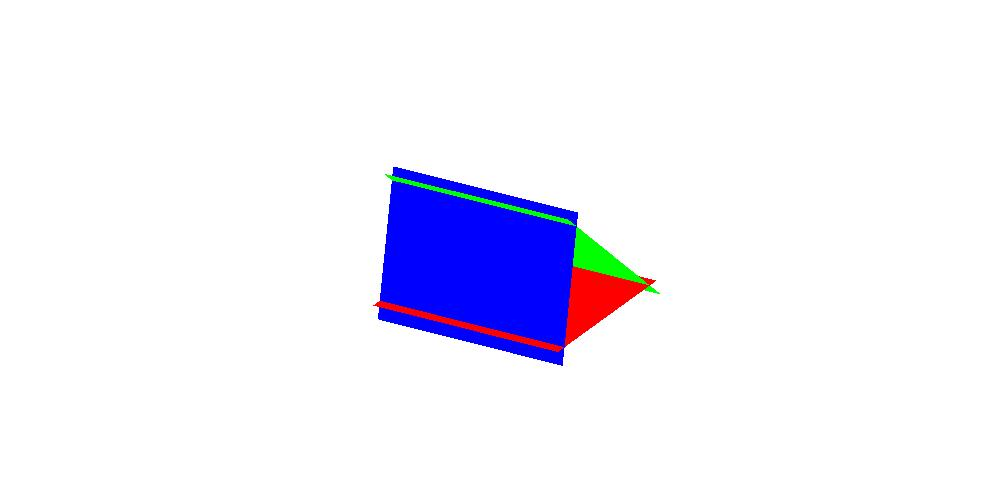
\includegraphics[scale=0.3,clip=true,
      trim=10cm 4.5cm 10cm 5.5cm]{images/toblerone}
 \]
 }
\end{frame}

\begin{frame}
 \frametitle{Example solution by row-reduction}
 
 We will solve the equations \vspace{-5ex}
 \begin{align*}
  a + b + c + d &= 4 \\
  a + b - c - d &= 0 \\
  a - b + c - d &= 0 \\
  a - b - c + d &= 0.
 \end{align*}
 \uc<2->{The corresponding augmented matrix can be row-reduced as follows:
 {\tiny \[
  \left[\begin{array}{cccc|c}
    1 &  1 &  1 &  1 & 4 \\
    1 &  1 & -1 & -1 & 0 \\
    1 & -1 &  1 & -1 & 0 \\
    1 & -1 & -1 &  1 & 0 
  \end{array}\right]
  \uc<3->{\xra{1}
  \left[\begin{array}{cccc|c}
    1 &  1 &  1 &  1 &  4 \\
    0 &  0 & -2 & -2 & -4 \\
    1 & -1 &  1 & -1 & 0 \\
    0 &  0 & -2 &  2 & 0 
  \end{array}\right]}
  \uc<4->{\xra{2}
  \left[\begin{array}{cccc|c}
    1 &  1 &  1 &  1 &  4 \\
    0 &  0 &  1 &  1 &  2 \\
    1 & -1 &  1 & -1 & 0 \\
    0 &  0 &  1 & -1 & 0 
  \end{array}\right]}
  \uc<5->{\xra{3}}
 \] \[
  \uc<5->{\left[\begin{array}{cccc|c}
    1 &  1 &  0 &  0 & 2 \\
    0 &  0 &  1 &  1 & 2 \\
    1 & -1 &  0 &  0 & 0 \\
    0 &  0 &  1 & -1 & 0 
  \end{array}\right]}
  \uc<6->{\xra{4}
  \left[\begin{array}{cccc|c}
    1 &  1 &  0 &  0 & 2 \\
    0 &  0 &  1 &  1 & 2 \\
    0 & -2 &  0 &  0 & -2 \\
    0 &  0 &  0 & -2 & -2 
  \end{array}\right]}
  \uc<7->{\xra{5}
  \left[\begin{array}{cccc|c}
    1 &  1 &  0 &  0 & 2 \\
    0 &  0 &  1 &  1 & 2 \\
    0 &  1 &  0 &  0 & 1 \\
    0 &  0 &  0 &  1 & 1 
  \end{array}\right]}
  \uc<8->{\xra{6}}
 \] \[
  \uc<8->{\left[\begin{array}{cccc|c}
    1 &  0 &  0 &  0 & 1 \\
    0 &  0 &  1 &  0 & 1 \\
    0 &  1 &  0 &  0 & 1 \\
    0 &  0 &  0 &  1 & 1 
  \end{array}\right]}
  \uc<9->{\xra{7}
  \left[\begin{array}{cccc|c}
    1 &  0 &  0 &  0 & 1 \\
    0 &  1 &  0 &  0 & 1 \\
    0 &  0 &  1 &  0 & 1 \\
    0 &  0 &  0 &  1 & 1 
  \end{array}\right]}
 \]}}
 \uc<3->{Subtract row 1 from row 2, and row 3 from row 4; }
 \uc<4->{Multiply rows 2 and 4 by $-1/2$; }
 \uc<5->{Subtract row 2 from row 1, and row 4 from row 3; }
 \uc<6->{Subtract row 1 from row 3, and row 2 from row 4; }
 \uc<7->{Multiply rows 3 and 4 by $-1/2$; }
 \uc<8->{Subtract row 3 from row 1, and row 4 from row 2; }
 \uc<9->{Exchange rows 2 and 3.}

 \uc<10->{The final matrix corresponds to the equations $a=1$, $b=1$, $c=1$ and
 $d=1$, which give the unique solution to the original system of
 equations.} 
\end{frame}

\begin{frame}
 \frametitle{Homogeneous systems}
 
 A system of linear equations is \emph{homogeneous} if the
 values on the right hand side are all zero.  \uc<2->{Example:
 \begin{align*}
  a+b+c+d+e+f &= 0 \\
  2a+2b+2c+2d-e-f &= 0 \\
  3a+3b-c-d-e-f &= 0
 \end{align*}}
 \uc<3->{The last column of the augmented matrix is zero all through the row
 reduction, so we need not write it in; we can work with the
 unaugmented matrix.}
 \uc<4->{\[ 
  \bbm
    1 &  1 &  1 &  1 &  1 &  1 \\
    2 &  2 &  2 &  2 & -1 & -1 \\
    3 &  3 & -1 & -1 & -1 & -1
  \ebm \uc<5->{\to \bbm
    \BLUE{1} &  \RED{1} &  \BLUE{0} &  \RED{0} &  \BLUE{0} &  \RED{0} \\ 
    \BLUE{0} &  \RED{0} &  \BLUE{1} &  \RED{1} &  \BLUE{0} &  \RED{0} \\ 
    \BLUE{0} &  \RED{0} &  \BLUE{0} &  \RED{0} &  \BLUE{1} &  \RED{1}
  \ebm}
 \]}
 \uc<6->{\[ \BLUE{a}+\RED{b} = 0 \hspace{5em}
    \BLUE{c}+\RED{d} = 0 \hspace{5em} 
    \BLUE{e}+\RED{f} = 0.
 \]}
 \uc<7->{Move the independent variables (from non-pivot columns) to the RHS:
 \[ \BLUE{a}=-\RED{b} \hspace{5em}
    \BLUE{c}=-\RED{d} \hspace{5em} 
    \BLUE{e}=-\RED{f}.
 \]}
 \uc<8->{If we prefer we can introduce new variables $\lm$, $\mu$ and $\nu$,
 and say that the general solution is
 \begin{align*}
  a &= -\lm & c &= -\mu & e &= -\nu \\
  b &=  \lm & d &=  \mu & f &=  \nu
 \end{align*}
 for arbitrary values of $\lm$, $\mu$ and $\nu$.}
\end{frame}

\begin{frame}\frametitle{Lecture 3}\end{frame}

\begin{frame}[t]
 \frametitle{Linear combinations}
 
 \begin{definition*}{\ref{defn-lincomb}}
  Let $v_1,\dotsc,v_k$ and $w$ be vectors in $\R^n$.  We say that $w$
  is a \emph{linear combination} of $v_1,\dotsc,v_k$ if there exist
  scalars $\lm_1,\dots,\lm_k$ such that
  \[ w = \lm_1v_1 + \dotsb + \lm_kv_k. \]
 \end{definition*}\vspace{-2ex}
 \uc<2->{\begin{example*}{\ref{eg-lincomb-i}}
  Consider the following vectors in $\R^4$:
  \[ v_1 = \bbm 1 \\ -1 \\ 0 \\ 0 \ebm \hspace{3em}
     v_2 = \bbm 0 \\ 1 \\ -1 \\ 0 \ebm \hspace{3em}
     v_3 = \bbm 0 \\ 0 \\ 1 \\ -1 \ebm \hspace{3em}
     w   = \bbm 1 \\ 10 \\ 100 \\ -111 \ebm 
  \] 
  \uc<3->{If we take $\lm_1=1$ and $\lm_2=11$ and $\lm_3=111$ we get 
  \[ \lm_1 v_1 + \lm_2 v_2 + \lm_3 v_3 = 
      \bbm 1 \\ -1 \\ 0 \\ 0 \ebm +
      \bbm 0 \\ 11 \\ -11 \\ 0 \ebm +
      \bbm 0 \\ 0 \\ 111 \\ -111 \ebm 
      \uc<4->{= \bbm 1 \\ 10 \\ 100 \\ -111 \ebm}
      \uc<5->{ = w}\uc<6->{,}
  \]}
  \uc<6->{which shows that $w$ is a linear combination of $v_1$, $v_2$ and
  $v_3$.}  
 \end{example*}}
\end{frame}


\begin{frame}[t]
 \frametitle{Linear combinations example}
 
 $w$ is a \emph{linear combination} of $v_1,\dotsc,v_k$ if there exist 
 scalars $\lm_1,\dots,\lm_k$ such that
 \[ w = \lm_1v_1 + \dotsb + \lm_kv_k. \]
 \reminderbar
 Consider the following vectors in $\R^4$:
 \[ v_1 = \bbm 0 \\ 1 \\  2 \\  3 \ebm \hspace{3em}
    v_2 = \bbm 0 \\ 1 \\  4 \\  9 \ebm \hspace{3em}
    v_3 = \bbm 0 \\ 1 \\  8 \\ 27 \ebm \hspace{3em}
    v_4 = \bbm 0 \\ 1 \\ 16 \\ 81 \ebm \hspace{3em}
    w = \bbm 1 \\ 1 \\ 1 \\ 1 \ebm.
 \]
 \uc<2->{Any linear combination of $v_1,\dotsc,v_4$ has the form 
 \[ \lm_1v_1 + \lm_2v_2 + \lm_3v_3 + \lm_4v_4 = 
     \bbm 0 \\ \lm_1+\lm_2+\lm_3+\lm_4 \\
          2\lm_1+4\lm_2+8\lm_3+16\lm_4 \\
          3\lm_1+9\lm_2+27\lm_3+81\lm_4 \ebm.
 \]}
 \uc<3->{Thus, the first component of any such linear combination is
  zero.}\\  
 \uc<4->{(You should be able to see this without writing out
 the whole formula.)}\\
 \uc<5->{As the first component of $w$ is not zero, we
 see that $w$ is \emph{not} a linear combination of $v_1,\dotsc,v_4$.}  
\end{frame}

\begin{frame}[t]
 \frametitle{Linear combinations example}
 
 $w$ is a \emph{linear combination} of $v_1,\dotsc,v_k$ if there exist 
 scalars $\lm_1,\dots,\lm_k$ such that
 \[ w = \lm_1v_1 + \dotsb + \lm_kv_k. \]
 \reminderbar
 Consider the following vectors in $\R^3$:
 \[ v_1 = \bbm 1 \\ 1 \\ 1 \ebm \hspace{1.5em}
    v_2 = \bbm 1 \\ 2 \\ 1 \ebm \hspace{1.5em}
    v_3 = \bbm 1 \\ 3 \\ 1 \ebm \hspace{1.5em}
    v_4 = \bbm 1 \\ 4 \\ 1 \ebm \hspace{1.5em}
    v_5 = \bbm 1 \\ 5 \\ 1 \ebm \hspace{1.5em}
    w   = \bbm -1 \\ 0 \\ 1 \ebm.
 \]
 \uc<2->{Any linear combination of $v_1,\dotsc,v_5$ has the form 
 \[ \lm_1v_1 + \dotsb + \lm_5v_5 = 
     \bbm \lm_1+\lm_2+\lm_3+\lm_4+\lm_5 \\
          \lm_1+2\lm_2+3\lm_3+4\lm_4+5\lm_5 \\
          \lm_1+\lm_2+\lm_3+\lm_4+\lm_5 \ebm.
 \]}
 \uc<3->{The first and last components of any such linear
 combination are the same.}\uc<4->{  Again, you should be able to see this
 without writing the full formula.}\uc<5->{  As the first and last components
 of $w$ are different, we see that $w$ is not a linear combination of
 $v_1,\dotsc,v_5$.  }
\end{frame}

\begin{frame}[t]
 \frametitle{Two vectors in $\R^3$ span a plane}
 \[ 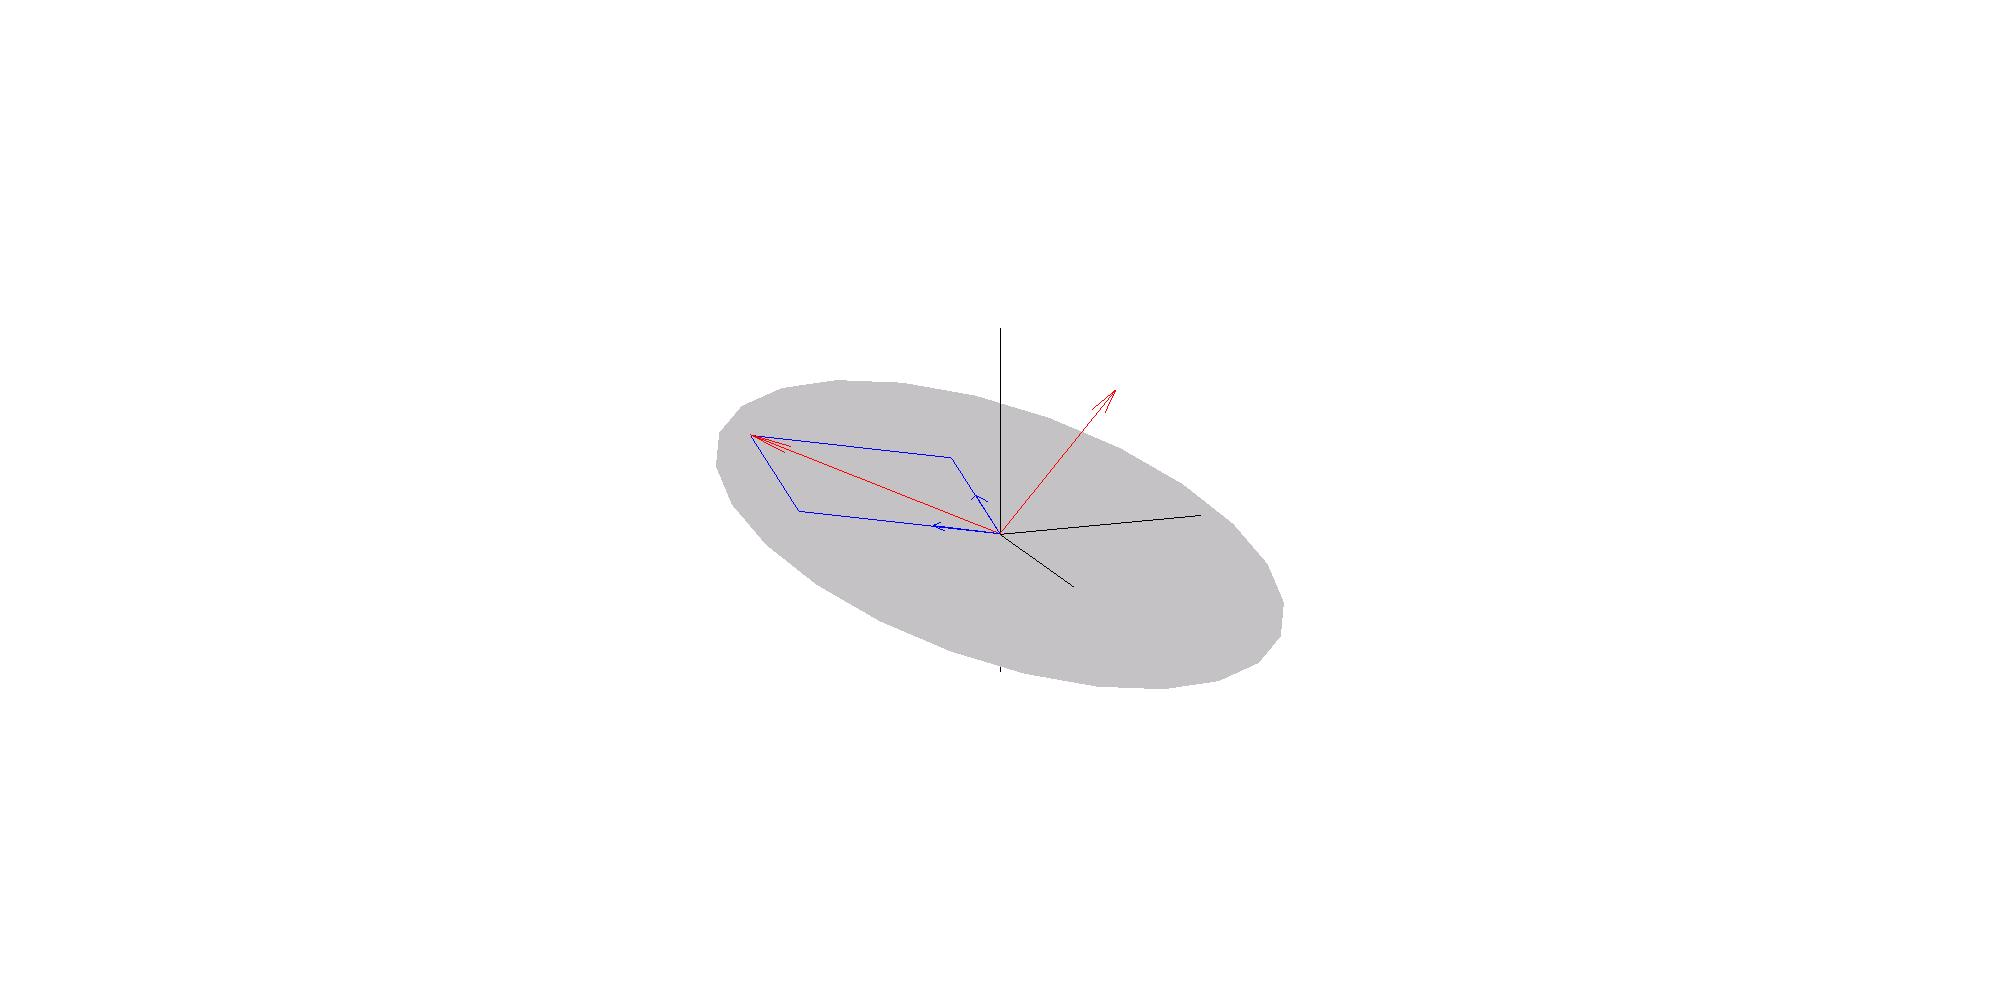
\includegraphics[scale=0.3,clip=true,
      trim=20cm 9cm 20cm 11cm]{images/plane_span}
 \]

 \uc<2->{Any vector that lies in the grey plane can be expressed
  as a linear combination of the two blue vectors.  }

 \uc<3->{Any vector that does not lie in the grey plane cannot be
  expressed as a linear combination of the two blue vectors.  }

\end{frame}

\begin{frame}[t]
 \frametitle{Method for finding linear combinations}
 
 Suppose we have vectors $v_1,\dotsc,v_k\in\R^n$ and another vector
 $w\in\R^n$\uc<2->{,\\
 and we want to express $w$ as a linear combination of the $v_i$}\\
 \uc<3->{(or show that this is not possible).  }

 \uc<4->{Let $A$ be the matrix whose columns are the vectors $v_i$: 
 \[ A = \left[\begin{array}{c|c|c} 
       v_1 & \cdots & v_k 
      \end{array}\right] \in M_{n\tm k}(\R).
 \]}
 \uc<5->{For any $k$-vector $\lm=\bbm\lm_1 & \dotsb & \lm_k\ebm^T$ we have
 \[ A\lm = 
     \left[\begin{array}{c|c|c} 
      v_1 & \cdots & v_k 
     \end{array}\right]
     \bbm \lm_1 \\ \vdots \\ \lm_k \ebm = 
     \lm_1 v_1 + \dotsb + \lm_k v_k
 \]}
 \uc<6->{Thus, to express $w$ as a linear combination of the $v_i$ is the same
 as to solve the vector equation $A\lm=w$}\uc<7->{, which we can do by
 row-reducing the augmented matrix 
 \[ B  = \left[\begin{array}{c|c} A & w\end{array}\right]
    \uc<8->{= \left[\begin{array}{c|c|c|c} 
                v_1 & \cdots & v_k & w 
              \end{array}\right]}
 \]}
\end{frame}

\begin{frame}[t]
 \frametitle{Example of finding a linear combination}
 
  Is $w$ a linear combination of $v_1$, $v_2$ and $v_3$?
  \[ v_1 = \bbm 11 \\ 11 \\ 1 \\ 1 \ebm \hspace{3em}
     v_2 = \bbm 1 \\ 11 \\ 11 \\ 1 \ebm \hspace{3em}
     v_3 = \bbm 1 \\ 1 \\ 11 \\ 11 \ebm \hspace{3em}
     w   = \bbm 121 \\ 221 \\ 1211 \\ 1111 \ebm.
  \]
  \uc<2->{We write down the relevant augmented matrix and row-reduce it:
  \[ 
   \left[\begin{array}{ccc|c}
    11 &  1 &  1 & 121 \\
    11 & 11 &  1 & 221 \\
     1 & 11 & 11 & 1211 \\
     1 &  1 & 11 & 1111
   \end{array}\right]
   \uc<3->{\hspace{-0.5em}\to\hspace{-0.5em}
   \left[\begin{array}{ccc|c}
     1 &  1 & 11 & 1111 \\
    11 &  1 &  1 & 121 \\
    11 & 11 &  1 & 221 \\
     1 & 11 & 11 & 1211
   \end{array}\right]}
   \uc<4->{\hspace{-0.5em}\to\hspace{-0.5em}
   \left[\begin{array}{ccc|c}
     1 &   1 &   11 & 1111 \\
     0 & -10 & -120 & -12100 \\
     0 &   0 & -120 & -12000 \\
     0 &  10 &    0 & 100
   \end{array}\right]}
  \] \[
   \uc<5->{\to
   \left[\begin{array}{ccc|c}
     1 &   1 &   11 & 1111 \\
     0 &   1 &   12 & 1210 \\
     0 &   0 &    1 & 100 \\
     0 &   1 &    0 & 10
   \end{array}\right]}
   \uc<6->{\to
   \left[\begin{array}{ccc|c}
     1 &   1 &    0 & 11 \\
     0 &   1 &    0 & 10 \\
     0 &   0 &    1 & 100 \\
     0 &   1 &    0 & 10
   \end{array}\right]}
   \uc<7->{\to
   \left[\begin{array}{ccc|c}
     1 &   0 &    0 & 1 \\
     0 &   1 &    0 & 10 \\
     0 &   0 &    1 & 100 \\
     0 &   0 &    0 & 0
   \end{array}\right]}
  \]}
  \uc<3->{Move the bottom row to the top;}
  \uc<4->{Subtract multiples of row 1 from the other rows;}
  \uc<5->{Divide rows 2,3 and 4 by $-10$, $-120$ and $10$;}
  \uc<6->{Subtract multiples of row 3 from the other rows;}
  \uc<7->{Subtract multiples of row 2 from the other rows.}
\end{frame}

\begin{frame}[t]
 \frametitle{Example of finding a linear combination}
  \vspace{-2ex}
  \[ v_1 = \bbm 11 \\ 11 \\ 1 \\ 1 \ebm \hspace{3em}
     v_2 = \bbm 1 \\ 11 \\ 11 \\ 1 \ebm \hspace{3em}
     v_3 = \bbm 1 \\ 1 \\ 11 \\ 11 \ebm \hspace{3em}
     w   = \bbm 121 \\ 221 \\ 1211 \\ 1111 \ebm.
  \]
  \[ 
   \left[\begin{array}{ccc|c}
    11 &  1 &  1 & 121 \\
    11 & 11 &  1 & 221 \\
     1 & 11 & 11 & 1211 \\
     1 &  1 & 11 & 1111
   \end{array}\right] \to \dotsb \to
   \left[\begin{array}{ccc|c}
     1 &   0 &    0 & 1 \\
     0 &   1 &    0 & 10 \\
     0 &   0 &    1 & 100 \\
     0 &   0 &    0 & 0
   \end{array}\right]
  \]
  \medskip

  \hrule

  \medskip

  \uc<2->{The final matrix corresponds to the system of equations
  \[ \lm_1 = 1 \hspace{3em}
     \lm_2 = 10 \hspace{3em}
     \lm_3 = 100 \hspace{3em}
      0 = 0
  \]}
  \uc<3->{so we conclude that $w = v_1 + 10 v_2 + 100 v_3$.}\\
  \uc<4->{In particular, $w$ can be expressed as a linear combination of $v_1$,
  $v_2$ and $v_3$.}  \\ \uc<5->{We can check the above equation directly:
  \[ v_1 + 10 v_2 + 100 v_3 = 
       \bbm  11 \\  11 \\    1 \\    1 \ebm +
       \bbm  10 \\ 110 \\  110 \\   10 \ebm +
       \bbm 100 \\ 100 \\ 1100 \\ 1100 \ebm 
     = \bbm 121 \\ 221 \\ 1211 \\ 1111 \ebm = w.
  \]}
\end{frame}

 
\begin{frame}[t]
 \frametitle{Example of not finding a linear combination}
 Is $b$ a linear combination of $a_1$, $a_2$ and $a_3$?
 \[ a_1 = \bbm 2 \\ -1 \\  0 \ebm \hspace{3em}
    a_2 = \bbm 3 \\  0 \\ -1 \ebm \hspace{3em}
    a_3 = \bbm 0 \\  3 \\ -2 \ebm \hspace{3em}
    b = \bbm 1 \\ 2 \\ 3 \ebm
 \]
 \uc<2->{We write down the relevant augmented matrix and row-reduce it:
 \[
  \left[\begin{array}{ccc|c}
    2 &  3 &  0 & 1 \\
   -1 &  0 &  3 & 2 \\
    0 & -1 & -2 & 3
  \end{array}\right]
  \uc<3->{\to
  \left[\begin{array}{ccc|c}
    1 &  0 & -3 & -2 \\
    0 &  1 &  2 & -3 \\
    2 &  3 &  0 &  1 
  \end{array}\right]}
  \uc<4->{\to
  \left[\begin{array}{ccc|c}
    1 &  0 & -3 & -2 \\
    0 &  1 &  2 & -3 \\
    0 &  3 &  6 &  5 
  \end{array}\right]}
  \uc<5->{\to}
 \] \[
  \uc<5->{\left[\begin{array}{ccc|c}
    1 &  0 & -3 & -2 \\
    0 &  1 &  2 & -3 \\
    0 &  0 &  0 & 14 
  \end{array}\right]}
  \uc<6->{\to
  \left[\begin{array}{ccc|c}
    1 &  0 & -3 & -2 \\
    0 &  1 &  2 & -3 \\
    0 &  0 &  0 &  1 
  \end{array}\right]}
  \uc<7->{\to
  \left[\begin{array}{ccc|c}
    1 &  0 & -3 &  0 \\
    0 &  1 &  2 &  0 \\
    0 &  0 &  0 &  1 
  \end{array}\right]}
 \]}
 \uc<3->{Move the top row to the bottom, and multiply the other two rows
 by $-1$;}
 \uc<4->{Subtract $2$ times row 1 from row 3;}
 \uc<5->{Subtract $3$ times row 2 from row 3;}
 \uc<6->{Divide row 3 by $14$;}
 \uc<7->{Subtract multiples of row 3 from rows 1 and 2.}
\end{frame}

\begin{frame}[t]
 \frametitle{Example of not finding a linear combination}
 \[ a_1 = \bbm 2 \\ -1 \\  0 \ebm \hspace{3em}
    a_2 = \bbm 3 \\  0 \\ -1 \ebm \hspace{3em}
    a_3 = \bbm 0 \\  3 \\ -2 \ebm \hspace{3em}
    b = \bbm 1 \\ 2 \\ 3 \ebm
 \]
 \[
  \left[\begin{array}{ccc|c}
    2 &  3 &  0 & 1 \\
   -1 &  0 &  3 & 2 \\
    0 & -1 & -2 & 3
  \end{array}\right]
  \to \dotsc \to
  \left[\begin{array}{ccc|c}
    1 &  0 & -3 &  0 \\
    0 &  1 &  2 &  0 \\
    0 &  0 &  0 &  1 
  \end{array}\right]
 \]
 \reminderbar
 \uc<2->{The final matrix has a pivot in the rightmost column,
  corresponding to the equation $0=1$.}\uc<3->{ This means that the
  equation $\lm_1a_1+\lm_2a_2+\lm_3a_3=b$ cannot be solved for
  $\lm_1$, $\lm_2$ and $\lm_3$}\uc<4->{, or in other words that $b$ is
  not a linear combination of $a_1$, $a_2$ and $a_3$.}

 \uc<5->{We can also see this in a more direct but less systematic
  way, as follows.}\uc<6->{  It is easy to check that $b.a_1=b.a_2=b.a_3=0$,
  which means that $b.(\lm_1a_1+\lm_2a_2+\lm_3a_3)=0$ for all possible
  choices of $\lm_1$, $\lm_2$ and $\lm_3$.}\uc<7->{ However, $b.b=14>0$, so
  $b$ cannot be equal to $\lm_1a_1+\lm_2a_2+\lm_3a_3$.}
\end{frame}


\begin{frame}[t]
 \frametitle{Linear independence}

 \begin{definition*}{\ref{defn-dependent}}
  Let $\CV=v_1,\dotsc,v_k$ be a list of vectors in $\R^n$.\\
  \uc<2->{A \emph{linear relation} between the $v_i$ is a relation of the
  form $\lm_1v_1+\dotsb+\lm_kv_k=0$, where $\lm_1,\dotsc,\lm_k$ are
  scalars.}  

  \medskip

  \uc<3->{For any list we have the trivial linear relation
  $0v_1+0v_2+\dotsb+0v_k=0$.}  \\
  \uc<4->{There may or may not be any nontrivial linear relations.}

  \medskip
  
  \uc<5->{If $\CV$ has a nontrivial linear relation, we say that it is
  \emph{(linearly) dependent}.\\}\uc<6->{  If the only linear relation on
  $\CV$ is the trivial one, we instead say that $\CV$ is \emph{(linearly)
   independent}.}
 \end{definition*}

 \medskip

 \uc<7->{\begin{example*}{\ref{eg-dep-i}}
  Consider the list $\CV$ given by 
  \[ v_1 = \bbm 1 \\ 1 \\ 0 \\ 0 \ebm \hspace{3em}
     v_2 = \bbm 0 \\ 0 \\ 1 \\ 1 \ebm \hspace{3em}
     v_3 = \bbm 1 \\ 0 \\ 0 \\ 1 \ebm \hspace{3em}
     v_4 = \bbm 0 \\ 1 \\ 1 \\ 0 \ebm.
  \]
  \uc<8->{There is a nontrivial linear relation $v_1+v_2-v_3-v_4=0$}\uc<9->{, so the
  list $\CV$ is dependent.}
 \end{example*}}
\end{frame}

\begin{frame}[t]
 \frametitle{Linear dependence example}
 The list $v_1,\dotsc,v_k$ is \emph{dependent} if there is a relation 
 $\lm_1v_1+\dotsb+\lm_kv_k=0$ with not all $\lm_i$ being zero.
 Otherwise, it is \emph{independent}.
 
 \medskip
 \hrule
 \medskip

 \begin{example*}{\ref{eg-dep-ii}}
  Consider the list $\CA$ given by 
  \[ a_1 = \bbm  1 \\  2 \ebm \hspace{3em}
     a_2 = \bbm 12 \\  1 \ebm \hspace{3em} 
     a_3 = \bbm -1 \\ -1 \ebm \hspace{3em} 
     a_4 = \bbm  3 \\  1 \ebm.
  \]
  \uc<2->{Just by writing it out, you can check that
  $3a_1 + a_2 + 3a_3 -4a_4 = 0$.} \\
  \only<3| handout:0>{
   \begin{center}
    \begin{tikzpicture}[scale=0.3]
     \fill( 0,0) circle(0.1); 
     \fill( 3,6) circle(0.1); 
     \fill(15,7) circle(0.1); 
     \fill(12,4) circle(0.1); 
     \draw[->, shorten >= 1pt] (0,0) -- (3,6);
     \draw[->, shorten >= 1pt] (3,6) -- (15,7);
     \draw[->, shorten >= 1pt] (15,7) -- (12,4);
     \draw[->, shorten >= 1pt] (12,4) -- (0,0);
     \draw ( 1.5,3.0) node[anchor=south east]{$\ss 3a_1$};
     \draw ( 9.0,6.5) node[anchor=south]{$\ss a_2$};
     \draw (13.5,5.5) node[anchor=north west]{$\ss 3a_3$};
     \draw ( 6.0,2.0) node[anchor=north]{$\ss -4a_4$};
    \end{tikzpicture}
   \end{center}\vspace{-30ex}}
  \uc<4->{This is a nontrivial linear relation on the list $\CA$, so $\CA$ is
  dependent.}  
 \end{example*}

 \medskip

 \uc<5->{\begin{example*}{\ref{eg-indep-i}}
  Claim: the following list $\CU$ is independent.
  \[ u_1 = \bbm \RED{1} & \RED{1} & 0 & 0 \ebm^T \hspace{3em}
     u_2 = \bbm 0 & \BLUE{1} & \BLUE{1} & 0 \ebm^T \hspace{3em}
     u_3 = \bbm 0 & 0 & \OLG{1} & \OLG{1} \ebm^T
  \]
  \uc<6->{Indeed, consider a linear
  relation $\lm_1u_1+\lm_2u_2+\lm_3u_3=0$.  }
  \uc<7->{This gives
  \[ \bbm \RED{\lm_1} \\ \RED{\lm_1}+\BLUE{\lm_2} \\ \BLUE{\lm_2}+\OLG{\lm_3} \\ \OLG{\lm_3} \ebm = 
     \bbm 0 \\ 0 \\ 0 \\ 0 \ebm ; \qquad
     \uc<8->{\lm_1=0;\qquad}
     \uc<9->{\lm_3=0;\qquad}
     \uc<10->{\lm_1+\lm_2=0;\qquad}
     \uc<11->{\lm_2=0.}
  \]}
  \uc<12->{As the only linear relation is the
  trivial one, we see that $\CU$ is independent.}
 \end{example*}}
\end{frame}

\begin{frame}[t]
 \frametitle{Pivots in every column}
 
 \uc<2->{\begin{definition*}{\ref{defn-wide}}
  Let $B$ be a $p\tm q$ matrix. \\
  We say that $B$ is
  \emph{wide} if $p<q$, or \emph{square} if $p=q$ or \emph{tall} if $p>q$.
  \[ \begin{array}{ccccc}
      \only<2-4>{\bbm 1 & 2 & 3 \\ 4 & 5 & 6 \ebm
     }\only<5| handout:0>{\bbm   1 & 0 & * \\ 0 & 1 & * \ebm
     }\only<6| handout:0>{\bbm   1 & * & 0 \\ 0 & 0 & 1 \ebm
     }\only<7| handout:0>{\bbm   1 & * & * \\ 0 & 0 & 0 \ebm
     }\only<8| handout:0>{\bbm   0 & 1 & 0 \\ 0 & 0 & 1 \ebm
     }\only<9-| handout:0>{\bbm   0 & 1 & * \\ 0 & 0 & 0 \ebm
     } & & 
      \only<1-9>{\bbm 1 & 2 & 1 \\ 2 & 3 & 2 \\ 1 & 2 & 1 \ebm
      }\only<10-| handout:0>{\bbm 1&0&0 \\ 0&1&0 \\ 0&0&1 \ebm} & & 
      \only<1-10>{\bbm 1 & 1 \\ 0 & 0 \\ 1 & 1 \ebm 
      }\only<11-| handout:0>{\bbm 1&0 \\ 0&1 \\ 0&0\ebm} \\
      \text{ wide } & & \text{ square } & & \text{ tall }
     \end{array}
  \]
 \end{definition*}}
 \uc<3->{\begin{lemma*}{\ref{lem-pivots-everywhere}}
  Let $B$ be a $p\tm q$ matrix in RREF.
  \begin{itemize}
   \item[(a)]<4-> If $B$ is wide then it is impossible for every column to
    contain a pivot.
   \item[(b)]<10-> If $B$ is square and every column contains a pivot then $B=I_q$.
   \item[(c)]<11-> If $B$ is tall  then the only way for every column to
    contain a pivot is if $B$ consists of $I_q$ with $(p-q)$ rows of
    zeros added at the bottom. 
    \[ B=\left[\begin{array}{cc} I_q \\ \hline 0_{(p-q)\tm q}\end{array}\right]\]
  \end{itemize}
 \end{lemma*}}
\end{frame}

\begin{frame}
 \frametitle{Checking dependence by row-reduction}
 
 \begin{method*}{\ref{meth-check-dependence}}
  Let $\CV=v_1,\dotsc,v_m$ be a list of vectors in $\R^n$.\\
  \uc<2->{We can check whether this list is dependent as follows.
  \begin{itemize}
   \item[(a)]<3-> Form the $n\tm m$ matrix
    $A = \left[\begin{array}{c|c|c}
               && \\
               v_1 & \dotsc & v_m \\
               && 
             \end{array}\right] 
    $
    whose columns are the vectors $v_i$.
   \item[(b)]<4-> Row reduce $A$ to get another $n\tm m$ matrix $B$ in
    RREF.  
   \item[(c)]<5-> If every column of $B$ contains a pivot
    (as on the previous slide) then $\CV$ is independent.  
   \item[(d)]<6-> If some column of $B$ has no pivot, then the list $\CV$
    is dependent.\uc<7->{  Moreover, we can find the coefficients $\lm_i$ in a
    nontrivial linear relation by solving the vector equation $B\lm=0$
    \uc<8->{(which is easy because $B$ is in RREF).}}
  \end{itemize}}
 \end{method*}
 \uc<9->{\begin{remark*}{\ref{rem-dependence-shortcut}}
  If $m>n$ then $\CV$ is automatically dependent and need not 
  do any more.\\
  \uc<10->{(Any list of $5$ vectors in $\R^3$ is dependent,
   any list of $10$ in $\R^9$ is dependent, 
  $\dotsc$.)} 

  \uc<11->{Indeed, in this case $B$ is wide, so it cannot have a pivot in
  every column.}\uc<12->{  This only tells us that there \textbf{exists} a
  nontrivial relation $\lm_1v_1+\dotsb+\lm_mv_m=0$}\uc<13->{, it does not tell
  us the coefficients $\lm_i$.}\uc<14->{  To find them we do need to go through
  the whole method as explained above.}
 \end{remark*}}
\end{frame}

\begin{frame}[t]
 \frametitle{Example of checking for (in)dependence}
 
 We previously considered the list
 \[ v_1 = \bbm 1 \\ 1 \\ 0 \\ 0 \ebm \hspace{3em}
    v_2 = \bbm 0 \\ 0 \\ 1 \\ 1 \ebm \hspace{3em}
    v_3 = \bbm 1 \\ 0 \\ 0 \\ 1 \ebm \hspace{3em}
    v_4 = \bbm 0 \\ 1 \\ 1 \\ 0 \ebm.
 \]
 \uc<2->{We can write down the corresponding matrix and row-reduce it as
 follows:
 \[ 
  \bbm 1 & 0 & 1 & 0 \\
       1 & 0 & 0 & 1 \\
       0 & 1 & 0 & 1 \\
       0 & 1 & 1 & 0
  \ebm \uc<3->{\xra{1}
  \bbm 1 & 0 & 1 & 0 \\
       0 & 0 &-1 & 1 \\
       0 & 1 & 0 & 1 \\
       0 & 0 & 1 &-1
  \ebm}\uc<4->{ \xra{2}
  \bbm 1 & 0 & 1 & 0 \\
       0 & 1 & 0 & 1 \\
       0 & 0 & 1 &-1 \\
       0 & 0 &-1 & 1 
  \ebm}\uc<5->{ \xra{3}
  \bbm 1 & 0 & 0 &\RED{ 1} \\
       0 & 1 & 0 &\RED{ 1} \\
       0 & 0 & 1 &\RED{-1} \\
       0 & 0 & 0 &\RED{ 0}
  \ebm }
 \]}
 \uc<6->{The end result has no pivot in the last column}\uc<7->{, so
  the original list is dependent.}\uc<8->{  To find a specific linear
  relation, we solve the equation  
 \[   \bbm 1 & 0 & 0 & 1 \\
           0 & 1 & 0 & 1 \\
           0 & 0 & 1 &-1 \\
           0 & 0 & 0 & 0
      \ebm
      \bbm \lm_1 \\ \lm_2 \\ \lm_3 \\ \lm_4 \ebm = 
      \bbm 0 \\ 0 \\ 0 \\ 0 \ebm 
      \hspace{4em}
      \begin{array}{l}
       \uc<9->{\lm_1=-\lm_4} \\ \uc<10->{\lm_2=-\lm_4} \\ \uc<11->{\lm_3=\lm_4} \\
       \uc<12->{\lm_4 \text{ arbitrary }}
      \end{array}
 \]}
 \uc<13->{Taking $\lm_4=1$ gives $(\lm_1,\lm_2,\lm_3,\lm_4)=(-1,-1,1,1)$}\uc<14->{,\\
 corresponding to the relation $-v_1-v_2+v_3+v_4=0$.}
\end{frame}

\begin{frame}[t]
 \frametitle{Example of checking for (in)dependence}
 We previously considered the list 
 \[ a_1 = \bbm  1 \\  2 \ebm \hspace{3em}
    a_2 = \bbm 12 \\  1 \ebm \hspace{3em} 
    a_3 = \bbm -1 \\ -1 \ebm \hspace{3em} 
    a_4 = \bbm  3 \\  1 \ebm.
 \]
 \uc<2->{Here we have $4$ vectors in $\R^2$, so they must be dependent.}
 \uc<3->{Thus, there exist nontrivial linear relations 
 $\lm_1a_1 + \lm_2a_2 + \lm_3a_3 + \lm_4a_4 = 0$.}\\
 \uc<4->{To actually find such a relation, we write down the corresponding
 matrix and row-reduce it as follows:
 \[ 
  \bbm 
   1 & 12 & -1 & 3 \\
   2 & 1  & -1 & 1 
  \ebm 
  \only<5| handout:0>{\xra{}
  \bbm
   1 &  12 & -1 & 3 \\
   0 & -23 &  1 & -5 
  \ebm}\only<6| handout:0>{\xra{}
  \GRAY{\bbm
   1 &  12 & -1 & 3 \\
   0 & -23 &  1 & -5 
  \ebm}}
  \uc<6->{\xra{}
  \bbm 
   1 &  12 & -1 & 3 \\
   0 &  1 & -1/23 & 5/23 
  \ebm}
  \uc<8->{\xra{}
  \bbm 
   1 &  0 & -11/23 & 9/23 \\
   0 &  1 & -1/23 & 5/23 
  \ebm}
 \]}
 \uc<9->{We now need to solve the matrix equation
 \[ \bbm 
     1 &  0 & -11/23 & 9/23 \\
     0 &  1 & -1/23 & 5/23 
    \ebm
    \bbm \lm_1 \\ \lm_2 \\ \lm_3 \\ \lm_4 \ebm =
    \bbm 0 \\ 0 \ebm
 \]}
 \uc<10->{This gives
 $\lm_1=\frac{11}{23}\lm_3-\frac{9}{23}\lm_4$ and
 $\lm_2=\frac{1}{23}\lm_3-\frac{5}{23}\lm_4$
 with $\lm_3$ and $\lm_4$ arbitrary.} \\
 \uc<11->{If we choose $\lm_3=23$ and
 $\lm_4=0$ we get $(\lm_1,\lm_2,\lm_3,\lm_4)=(11,1,23,0)$}\uc<12->{ so we have a
 relation $11 a_1 + a_2 + 23 a_3 + 0 a_4 = 0$.}
\end{frame}


\begin{frame}[t]
 \frametitle{Example of checking for (in)dependence}

 We previously considered the list $\CU$ given by 
 \[ u_1 = \bbm 1 \\ 1 \\ 0 \\ 0 \ebm \hspace{3em}
    u_2 = \bbm 0 \\ 1 \\ 1 \\ 0 \ebm \hspace{3em}
    u_3 = \bbm 0 \\ 0 \\ 1 \\ 1 \ebm.
 \]
 \uc<2->{We can write down the corresponding matrix and row-reduce it as
 follows: 
 \[ 
  \bbm 
   1 & 0 & 0 \\
   1 & 1 & 0 \\
   0 & 1 & 1 \\
   0 & 0 & 1
  \ebm 
  \uc<3->{\to 
  \bbm 
   1 & 0 & 0 \\
   0 & 1 & 0 \\
   0 & 1 & 1 \\
   0 & 0 & 1
  \ebm }
  \uc<4->{\to 
  \bbm 
   1 & 0 & 0 \\
   0 & 1 & 0 \\
   0 & 0 & 1 \\
   0 & 0 & 1
  \ebm }
  \uc<5->{\to 
  \left[\begin{array}{ccc}
   1 & 0 & 0 \\
   0 & 1 & 0 \\
   0 & 0 & 1 \\ \hline
   0 & 0 & 0
  \end{array}\right]}
 \]}
 \uc<6->{The final matrix has a pivot in every column.
 It follows that the list $\CU$ is independent. }
\end{frame}

\begin{frame}[t]
 \frametitle{Proof of correctness of the method}
 
 \uc<2->{Put $A = \left[\begin{array}{c|c|c}
              && \\
              v_1 & \cdots & v_m \\
              && 
        \end{array}\right] 
 $
 as in step~(a)}\uc<3->{, and let $B$ be the RREF form of $A$.}
 \uc<4->{Note that for any vector
 $\lm=\bbm \lm_1 & \dotsc & \lm_m\ebm^T\in\R^m$, we have 
 \[ A\lm = 
     \left[\begin{array}{c|c|c}
              && \\
              v_1 & \cdots & v_m \\
              && 
     \end{array}\right] 
     \bbm \lm_1 \\ \vdots \\ \lm_m \ebm = 
     \lm_1v_1 + \dotsb + \lm_mv_m.
 \]}
 \uc<5->{Thus, linear relations on our list are just the same as solutions to
 the homogeneous equation $A\lm=0$.}\uc<6->{  We saw earlier that these are the
 same as solutions to the equation $B\lm=0$}\uc<7->{, which can be found by the
 standard method for RREF equations.}\uc<8->{  If there is a pivot in every
 column then none of the variables $\lm_i$ is independent}\uc<9->{, so the only
 solution is $\lm_1=\lm_2=\dotsb=\lm_m=0$.}\uc<10->{  Thus, the only linear
 relation on $\CV$ is the trivial one}\uc<11->{, which means that the list $\CV$
 is linearly independent.}

 \uc<12->{Suppose instead that some column (the $k$'th one, say) does not
 contain a pivot.}\uc<13->{  Then the variable $\lm_k$ will be independent, so
 we can choose $\lm_k=1$.}\uc<14->{  This will give us a nonzero to solution to
 $B\lm=0$}\uc<15->{, or equivalently $A\lm=0$}\uc<16->{, corresponding to a nontrivial
 linear relation on $\CV$.}\uc<17->{  This shows that $\CV$ is linearly
 dependent.}
\end{frame}

\begin{frame}\frametitle{Lecture 4}\end{frame}

\begin{frame}[t]
 \frametitle{Spanning}
 
 \begin{definition*}{\ref{defn-spanning-list}}
  Suppose we have a list $\CV=v_1,\dotsc,v_m$ of vectors in $\R^n$.  
  \uc<2->{Then $\CV$ \emph{spans} $\R^n$ if \textbf{every} vector in
  $\R^n$ can be expressed as a linear combination of $v_1,\dotsc,v_m$.}
 \end{definition*}

 \medskip

 \uc<3->{\begin{example*}{\ref{eg-not-span-i}}
  Consider the list $\CV=v_1,v_2,v_3,v_4$, where \vspace{-1ex}
  \[ v_1 = \bbm 0 \\ 1 \\  2 \\  3 \ebm \hspace{3em}
     v_2 = \bbm 0 \\ 1 \\  4 \\  9 \ebm \hspace{3em}
     v_3 = \bbm 0 \\ 1 \\  8 \\ 27 \ebm \hspace{3em}
     v_4 = \bbm 0 \\ 1 \\ 16 \\ 81 \ebm
  \] \vspace{-1ex}

  \uc<4->{Previously we saw that the vector
  $w=\bbm 1 & 1 & 1 & 1\ebm^T$ is not a linear combination of this
  list}\uc<5->{, so the list $\CV$ does not span $\R^4$.}
 \end{example*}}

 \medskip

 \uc<6->{\begin{example*}{\ref{eg-not-span-ii}}
  Consider the list $\CV=v_1,v_2,v_3,v_4,v_5$, where\vspace{-1ex}
  \[ v_1 = \bbm 1 \\ 1 \\ 1 \ebm \hspace{3em}
     v_2 = \bbm 1 \\ 2 \\ 1 \ebm \hspace{3em}
     v_3 = \bbm 1 \\ 3 \\ 1 \ebm \hspace{3em}
     v_4 = \bbm 1 \\ 4 \\ 1 \ebm \hspace{3em}
     v_5 = \bbm 1 \\ 5 \\ 1 \ebm. 
  \]\vspace{-1ex}

  \uc<7->{Previously we saw that the vector
  $w=\bbm -1 & 0 & 1 \ebm^T$ is not a linear combination of this
  list}\uc<8->{, so the list $\CV$ does not span $\R^3$.}
 \end{example*}}
\end{frame}

\begin{frame}[t]
 \frametitle{Spanning example}
 
 Consider the list $\CU=u_1,u_2,u_3$, where
 \[ u_1 = \bbm 1 \\ 1 \\ 0 \ebm \hspace{3em}
    u_2 = \bbm 1 \\ 0 \\ 1 \ebm \hspace{3em}
    u_3 = \bbm 0 \\ 1 \\ 1 \ebm.
 \]
 \uc<2->{We will show that these span $\R^3$.}\uc<3->{  Indeed, for any vector
 $v=\bbm x & y & z\ebm^T\in\R^3$ we can put
 \[ \lm_1 = \frac{ x+y-z}{2} \hspace{4em}
    \lm_2 = \frac{ x-y+z}{2} \hspace{4em}
    \lm_3 = \frac{-x+y+z}{2}
 \]}\uc<4->{
 and we find that
 \def\x{\RED{x}}\def\y{\BLUE{y}}\def\z{\OLG{z}}
 \begin{align*}
  \lm_1u_1+\lm_2u_2+\lm_3u_3
    &\uc<5->{=
   \bbm (\x+\y-\z)/2 \\ (\x+\y-\z)/2 \\ 0 \ebm + 
   \bbm (\x-\y+\z)/2 \\ 0 \\ (\x-\y+\z)/2 \ebm +
   \bbm 0 \\ (-\x+\y+\z)/2 \\ (-\x+\y+\z)/2 \ebm} \\
    &\uc<6->{= 
   \bbm (\x+\y-\z+\x-\y+\z)/2 \\
        (\x+\y-\z-\x+\y+\z)/2 \\
        (\x-\y+\z-\x+\y+\z)/2 \ebm }\uc<7->{
    = \bbm \x \\ \y \\ \z \ebm}\uc<8->{ = v.}
 \end{align*}}
 \uc<9->{This expresses $v$ as a linear combination of the list $\CU$, as
 required.} 
\end{frame}

\begin{frame}[t]
 \frametitle{Spanning example}
 
 Consider the list $\CA=a_1,a_2,a_3$ where
 \[ a_1 = \bbm 1 \\ 2 \ebm \hspace{3em}
    a_2 = \bbm 2 \\ 3 \ebm \hspace{3em}
    a_3 = \bbm 3 \\ 5 \ebm.  
 \]
 \uc<2->{Let $v=\bbm x \\ y\ebm$ be an arbitrary vector in $\R^2$.}\uc<3->{  Note that 
 \[ (2y-4x)\bbm 1 \\ 2 \ebm + (x-y)\bbm 2\\ 3\ebm + x\bbm 3\\5 \ebm 
  \uc<4->{= \bbm 2y-4x \\ 4y-8x \ebm + 
     \bbm 2x-2y \\ 3x-3y \ebm + 
     \bbm 3x \\ 5x \ebm }\uc<5->{
  = \bbm x \\ y \ebm}
 \]}
 \uc<6->{or in other words
 \[ v = (2y-4x)a_1 + (x-y)a_2 + x a_3. \]}\uc<7->{
 This expresses an arbitrary $v\in\R^2$ as a linear combination
 of $a_1$, $a_2$ and $a_3$}\uc<8->{, \\ proving that the list $\CA$ spans $\R^2$.}

 \bigskip

 \uc<9->{In this case there are actually many different ways in which we can
 express $v$ as a linear combination of $a_1$, $a_2$ and $a_3$.}\uc<10->{
 Another one is
 \[ v = (y-3x)a_1 + (2x-2y)a_2 + y a_3. \]}
\end{frame}

\begin{frame}[t]
 \frametitle{Checking spanning by row-reduction}

 \begin{method*}{\ref{meth-check-span}}
  Let $\CV=v_1,\dotsc,v_m$ be a list of vectors in $\R^n$.  \\
  \uc<2->{We can check whether this list spans $\R^n$ as follows.}
  \begin{itemize}
   \item[(a)]<3-> Form the $m\tm n$ matrix
    $ C = \left[\begin{array}{ccc}
               & v_1^T & \\ \hline & \vdots & \\ \hline & v_m^T &
             \end{array}\right] 
    $
    whose rows are the $v_i^T$.
   \item[(b)]<4-> Row reduce $C$ to get another $m\tm n$ matrix $D$ in
    RREF.
   \item[(c)]<5-> If every column of $D$ contains a pivot (so
    $D=\left[\begin{array}{cc} I_n \\ \hline 0_{(m-n)\tm n}\end{array}\right]$)
    then $\CV$ spans $\R^n$.
   \item[(d)]<6-> If some column of $D$ has no pivot, then the list $\CV$
    does not span $\R^n$.
  \end{itemize}
 \end{method*}
 \uc<7->{\begin{remark*}{\ref{rem-dual-methods}}
  This is almost exactly the same as the method for checking
  independence\uc<8->{, except that here we start by building a matrix $C$
  whose rows are $v_i^T$, instead of building a matrix $A$ whose
  columns are $v_i$.}\uc<9->{ These are transposes of each other:
  $A=C^T$ and $C=A^T$.}

  \medskip

  \uc<10->{  \textbf{Warning:} transposing
  does not interact well with row-reduction, so the matrix $D$ is
  \textbf{not} the transpose of $B$.}
 \end{remark*}}
\end{frame}

\begin{frame}[t]
 \frametitle{Example of spanning check}
 
 Consider the list 
 \[ v_1 = \bbm \RED{0} \\ \RED{1} \\  \RED{2} \\  \RED{3} \ebm \hspace{3em}
    v_2 = \bbm \BLUE{0} \\ \BLUE{1} \\  \BLUE{4} \\  \BLUE{9} \ebm \hspace{3em}
    v_3 = \bbm \OLG{0} \\ \OLG{1} \\  \OLG{8} \\ \OLG{27} \ebm \hspace{3em}
    v_4 = \bbm \ORANGE{0} \\ \ORANGE{1} \\ \ORANGE{16} \\ \ORANGE{81} \ebm
 \]
 \uc<2->{The relevant matrix is  
 $ C   = \bbm 
           \RED{0} & \RED{1} &  \RED{2} &  \RED{3} \\
           \BLUE{0} & \BLUE{1} &  \BLUE{4} &  \BLUE{9} \\
           \OLG{0} & \OLG{1} &  \OLG{8} & \OLG{27} \\
           \ORANGE{0} & \ORANGE{1} & \ORANGE{16} & \ORANGE{81} 
          \ebm
 $}

 \medskip

 \uc<3->{The first column is zero}\uc<4->{, and will remain zero no
  matter what row operations we perform.}\uc<5->{  Thus $C$ cannot
  reduce to the identity matrix}\uc<6->{, so $\CV$ does not
  span}\uc<7->{ (as we already saw by a different method).}\uc<8->{
  In fact the row-reduction is 
 \[ C \to \bbm 0 & 1 & 0 & 0 \\
               0 & 0 & 1 & 0 \\
               0 & 0 & 0 & 1 \\
               0 & 0 & 0 & 0 \ebm
 \]}
 \uc<9->{but it is not really necessary to go through the whole calculation.}
\end{frame}

\begin{frame}[t]
 \frametitle{Example of spanning check}
 
 Consider the list $\CV$ given by 
 \[ v_1 = \bbm \RED{1} \\ \RED{1} \\ \RED{1} \ebm \hspace{3em}
    v_2 = \bbm \BLUE{1} \\ \BLUE{2} \\ \BLUE{1} \ebm \hspace{3em}
    v_3 = \bbm \OLG{1} \\ \OLG{3} \\ \OLG{1} \ebm \hspace{3em}
    v_4 = \bbm \MAGENTA{1} \\ \MAGENTA{4} \\ \MAGENTA{1} \ebm \hspace{3em}
    v_5 = \bbm \CYAN{1} \\ \CYAN{5} \\ \CYAN{1} \ebm. 
 \]
 \uc<2->{The relevant row-reduction is
 \[
 \bbm \RED{1}     & \RED{1}     & \RED{1}  \\
      \BLUE{1}    & \BLUE{2}    & \BLUE{1} \\ 
      \OLG{1}     & \OLG{3}     & \OLG{1}  \\ 
      \MAGENTA{1} & \MAGENTA{4} & \MAGENTA{1} \\
      \CYAN{1}    & \CYAN{5}    & \CYAN{1} \ebm 
 \uc<3->{\to 
 \bbm 1 & 1 & 1 \\ 0 & 1 & 0 \\ 0 & 2 & 0 \\ 0 & 3 & 0 \\ 0 & 4 & 0 \ebm }
 \uc<4->{\to 
  \left[\begin{array}{ccc}
    1 & 0 & 1 \\
    0 & 1 & 0 \\
    0 & 0 & 0 \\ \hline
    0 & 0 & 0 \\
    0 & 0 & 0 
  \end{array}\right] }
 \]}
 \uc<5->{At the end of the process the last column does not contain a pivot}
 \uc<6->{(so the top $3\tm 3$ block is not the identity)}\uc<7->{,
 so $\CV$ does not span $\R^3$.}\uc<8->{  Again, we saw this earlier by a
 different method.}
\end{frame}

\begin{frame}[t]
 \frametitle{Example of spanning check}
 
 \uc<2->{For the list 
 \[ \CA = \bbm \RED{2} \\ \RED{-1} \\  \RED{0} \ebm, \qquad
          \bbm \BLUE{3} \\  \BLUE{0} \\ \BLUE{-1} \ebm, \qquad
          \bbm \OLG{0} \\  \OLG{3} \\ \OLG{-2} \ebm
 \]}\uc<3->{
 the relevant row-reduction is 
 \[ \bbm \RED{2} & \RED{-1} & \RED{0} \\
         \BLUE{3} & \BLUE{0} & \BLUE{-1} \\ 
         \OLG{0} & \OLG{3} & \OLG{-2} \ebm \uc<4->{\to
    \bbm 1 & -\half & 0 \\ 3 & 0 & -1 \\ 0 & 3 & -2 \ebm}\uc<5->{ \to
    \bbm 1 & -\half & 0 \\ 0 & \tfrac{3}{2} & -1 \\ 0 & 3 & -2 \ebm}
    \uc<6->{\to}
 \]}
 \[ \uc<6->{\bbm 1 & -\half & 0 \\ 0 & 1 & -\tfrac{2}{3} \\ 0 & 0 & 0 \ebm}
    \uc<7->{\to
    \bbm 1 & 0 & -\tfrac{1}{3} \\ 0 & 1 & -\tfrac{2}{3} \\ 0 & 0 & 0 \ebm.}
 \]
 \uc<8->{In the last matrix the third column has no pivot, so the list does
 not span.} 
\end{frame}

\begin{frame}[t]
 \frametitle{Example of spanning check}
 
 Consider the list $\CU=u_1,u_2,u_3$
 \[ u_1 = \bbm \RED{1} \\ \RED{1} \\ \RED{0} \ebm \hspace{3em}
    u_2 = \bbm \BLUE{1} \\ \BLUE{0} \\ \BLUE{1} \ebm \hspace{3em}
    u_3 = \bbm \OLG{0} \\ \OLG{1} \\ \OLG{1} \ebm.
 \]
 \uc<2->{The relevant row-reduction is
 \[             \bbm \RED{1}  &  \RED{1} & \RED{0} \\ 
                     \BLUE{1} & \BLUE{0} & \BLUE{1} \\
                     \OLG{0}  &  \OLG{1} & \OLG{1} \ebm 
    \uc<3->{\to \bbm 1 & 1 & 0 \\ 0 & -1 &  1 \\ 0 & 1 & 1 \ebm}
    \uc<4->{\to \bbm 1 & 1 & 0 \\ 0 &  1 & -1 \\ 0 & 0 & 2 \ebm}
    \uc<5->{\to}
 \]\[
    \uc<5->{    \bbm 1 & 1 & 0 \\ 0 &  1 &  0 \\ 0 & 0 & 1 \ebm}
    \uc<6->{\to \bbm 1 & 0 & 0 \\ 0 &  1 &  0 \\ 0 & 0 & 1 \ebm}
 \]}
 \uc<7->{The end result is the identity matrix, so the list $\CU$ spans
 $\R^3$. }
\end{frame}

\begin{frame}[t]
 \frametitle{Example of spanning check}
 
 Consider the list
 $\CA=\bbm \RED{1}\\\RED{2}\ebm,\;\bbm \BLUE{2}\\\BLUE{3}\ebm,\;\bbm \OLG{3}\\\OLG{5}\ebm$.
 \uc<2->{The relevant row-reduction is
 \[ \bbm \RED{1} & \RED{2} \\ \BLUE{2} & \BLUE{3} \\ \OLG{3} & \OLG{5} \ebm 
    \uc<3->{\to \bbm 1 & 2 \\ 0 & -1 \\ 0 & -1 \ebm }
    \uc<4->{\to \bbm 1 & 2 \\ 0 &  1 \\ 0 & -1 \ebm }
    \uc<5->{\to \left[\begin{array}{cc}
                   1 & 0 \\ 0 &  1 \\ \hline 0 & 0
                \end{array}\right] }
 \]} 
 \uc<6->{In the last matrix, the top $2\tm 2$ block is the identity.}
 \uc<7->{This means that the list $\CA$ spans $\R^2$.}
\end{frame}

\begin{frame}[t]
 \frametitle{Proof of correctness of the method}

 \uc<2->{\begin{lemma*}{\ref{lem-span-invariant}}
  Let $C$ be an $m\tm n$ matrix, and let $C'$ be obtained from $C$ by a
  single elementary row operation.  Let $s$ be a row vector of length
  $n$.  Then $s$ can be expressed as a linear combination of the rows
  of $C$ if and only if it can be expressed as a linear combination of
  the rows of $C'$. 
 \end{lemma*}}

 \uc<3->{\noindent{\large\BLUE{Proof:}}
 Let the rows of $C$ be $r_1,\dotsc,r_m$.  \uc<4->{Suppose that $s$ is a
 linear combination of these rows, say 
 \[ s=\lm_1r_1+\lm_2r_2+\lm_3r_3+\dotsb+\lm_mr_m. \]}
 \begin{itemize}
  \item[(a)]<5-> Suppose that $C'$ is obtained from $C$ by swapping the
   first two rows\uc<6->{, so the rows of $C'$ are $r_2,r_1,r_3,\dotsc,r_m$.}  
   \uc<7->{The sequence of numbers $\lm_2,\lm_1,\lm_3,\dotsc,\lm_m$ satisfies 
   \[ s=\lm_2r_2+\lm_1r_1+\lm_3r_3+\dotsb+\lm_mr_m\uc<8->{,} \]}
   \uc<8->{which expresses $s$ as a linear combination of the rows of
    $C'$.}\uc<9->{  The argument is essentially the same if we exchange any
    other pair of rows.}
  \end{itemize}}
\end{frame}

\begin{frame}[t]
 \frametitle{Proof of correctness of the method}
 $C\in M_{m\tm n}(\R)$; $C'$ obtained from $C$ by a single row
 operation; $s$ a row vector of length $n$.  Claim: $s$ is a linear
 combination of rows of $C$ iff it is a linear combination of rows of
 $C'$.
 \reminderbar
 \begin{itemize}
  \item[(b)]<2-> Suppose instead that $C'$ is obtained from $C$ by
    multiplying the first row by a nonzero scalar $u$\uc<3->{, so the rows of
    $C'$ are $ur_1,r_2,\dotsc,r_m$.}\uc<4->{  The sequence of numbers
    $u^{-1}\lm_1,\lm_2,\dotsc,\lm_m$ then satisfies 
    \[ s = (u^{-1}\lm_1)(ur_1)+\lm_2u_2+\dotsb+\lm_mr_m\uc<5->{,} \]}
    \uc<5->{which expresses $s$ as a linear combination of the rows of
     $C'$.}\uc<6->{The argument is essentially the same if we multiply
     any other row by a constant. }
   \item[(c)]<7-> Suppose instead that $C'$ is obtained from $C$ by adding
    $u$ times the second row to the first row\uc<8->{, so the rows of $C'$ are
    $r_1+ur_2,r_2,r_3,\dotsc,r_m$.}\uc<9->{  The sequence of numbers
    $\lm_1,\lm_2-u\lm_1,\lm_3,\dotsc,\lm_n$ then satisfies 
    \[ \lm_1(r_1+ur_2)+(\lm_2-u\lm_1)r_2+\lm_3r_3+\dotsb+\lm_mr_m =
        \lm_1r_1+\lm_2r_2+\dotsb+\lm_mr_m=s\uc<10->{,}
    \]}
    \uc<10->{which expresses $s$ as a linear combination of the rows
     of $C'$.}\uc<11->{  The argument is essentially the same if add a
     multiple of any row to any other row.}
  \end{itemize}
\end{frame}

\begin{frame}[t]
 \frametitle{Proof of correctness of the method}
 $C\in M_{m\tm n}(\R)$; $C'$ obtained from $C$ by a single row
 operation; $s$ a row vector of length $n$.  Claim: $s$ is a linear
 combination of rows of $C$ iff it is a linear combination of rows of
 $C'$.

 \medskip
 \hrule
 \medskip

 \uc<2->{We have now proved half of the lemma: if $s$ is a linear
  combination of the rows of $C$, then it is also a linear combination
  of the rows of $C'$.}\uc<3->{  We also need to prove the converse: if $s$ is
  a linear combination of the rows of $C'$, then it is also a linear
  combination of the rows of $C$.}\uc<4->{  We will only treat case~(c), and
  leave the other two cases as an exercise.}\uc<5->{  The rows of $C'$ are then
  $r_1+ur_2,r_2,r_3,\dotsc,r_m$.}\uc<6->{ As $s$ is a linear combination of
  these rows, we have $s=\mu_1(r_1+ur_2)+\mu_2r_2+\dotsb+\mu_mr_m$ for
  some numbers $\mu_1,\dotsc,\mu_m$.}\uc<7->{  Now the sequence of numbers
  $\mu_1,(\mu_2+u\mu_1),\mu_3,\dotsc,\mu_m$ satisfies
 \[ s = \mu_1r_1+(\mu_2+u\mu_1)r_2+\mu_3r_3+\dotsb+\mu_mr_m\uc<8->{,} \]}
 \uc<8->{which expresses $s$ as a linear combination of the rows of $C$.}
\end{frame}

\begin{frame}[t]
 \frametitle{Proof of correctness of the method}
 $C\in M_{m\tm n}(\R)$; $C'$ obtained from $C$ by a single row
 operation; $s$ a row vector of length $n$.  Claim: $s$ is a linear
 combination of rows of $C$ iff it is a linear combination of rows of
 $C'$.

 \medskip
 \hrule
 \vspace{6ex}

 \begin{corollary*}{\ref{cor-span-invariant}}
  Let $C$ be an $m\tm n$ matrix, and let $D$ be obtained from $C$ by a
  sequence of elementary row operation.  Let $s$ be a row vector of length
  $n$.  Then $s$ can be expressed as a linear combination of the rows
  of $C$ if and only if it can be expressed as a linear combination of
  the rows of $D$.  
 \end{corollary*}
 \begin{proof}
  Just apply the lemma to each step in the row-reduction sequence.
 \end{proof}
\end{frame}

\begin{frame}[t]
 \frametitle{Proof of correctness of the method}

 \begin{lemma*}{\ref{lem-check-span-RREF}}
  Let $D$ be an $m\tm n$ matrix in RREF.  
  \begin{itemize}
   \uc<2->{\item[(a)] Suppose that every column of $D$ contains a pivot, so
    $D=\left[\begin{array}{cc} I_n \\ \hline 0_{(m-n)\tm n}\end{array}\right]$. 
    Then every row vector of length $n$ can be expressed as a linear
    combination of the rows of $D$.} 
   \only<3>{\item[(b)] Suppose instead that the $k$'th column of $D$ does not
    contain a pivot.  Then the $k$'th standard basis vector $e_k$
    \textbf{cannot} be expressed as a linear combination of the rows
    of $D$. }
  \end{itemize}
 \end{lemma*}

 \uc<4->{{\large\BLUE{Proof of (a):}}
 In this case the first $n$ rows are the standard basis vectors 
 \begin{align*}
  r_1 &= e_1^T = \bbm 1 & 0 & 0 & \cdots & 0 \ebm \\
  r_2 &= e_2^T = \bbm 0 & 1 & 0 & \cdots & 0 \ebm \dotsb \\
  r_n &= e_n^T = \bbm 0 & 0 & 0 & \cdots & 1 \ebm 
 \end{align*}
 and $r_i=0$ for $i>n$.  This means that any row vector
 $v=\bbm v_1 & v_2 & \cdots & v_n\ebm$ can be expressed as \vspace{-4ex}
 \begin{align*}
  v =& \bbm v_1 & 0 & 0 & \cdots & 0 \ebm + \\
     & \bbm 0 & v_2 & 0 & \cdots & 0 \ebm + \dotsb + \\
     & \bbm 0 & 0 & 0 & \cdots & v_n \ebm  \\
    =& v_1r_1 + v_2r_2 + v_3r_3 + \dotsb + v_nr_n,
 \end{align*}
 which is a linear combination of the rows of $D$.}
\end{frame}

\begin{frame}[t]
 \frametitle{Proof of correctness of the method}

 {\large\BLUE{Lemma:}}
  Let $D$ be an $m\tm n$ matrix in RREF.  
  \begin{itemize}
   \only<1>{\item[(a)] Suppose that every column of $D$ contains a pivot, so
    $D=\left[\begin{array}{cc} I_n \\ \hline 0_{(m-n)\tm n}\end{array}\right]$. 
    Then every row vector of length $n$ can be expressed as a linear
    combination of the rows of $D$.} 
   \item[(b)] Suppose instead that the $k$'th column of $D$ does not
    contain a pivot.  Then the $k$'th standard basis vector $e_k$
    \textbf{cannot} be expressed as a linear combination of the rows
    of $D$.
  \end{itemize}

 \uc<3->{{\large\BLUE{Example for proof of (b):}}
 \uc<4->{Consider the matrix 
 \[ D = \bbm 0 & \RED{1} & \BLUE{2} & \OLG{3} & 0 & \CYAN{4} & \ORANGE{5} & 0 \\
             0 & 0 & 0 & 0 & \MAGENTA{1} & \CYAN{6} & \ORANGE{7} & 0 \\
             0 & 0 & 0 & 0 & 0 & 0 & 0 & \VIOLET{1} \ebm
 \]}
 \uc<5->{This is in RREF, with pivots in columns $\RED{2}$, $\MAGENTA{5}$ and $8$.}
 \uc<6->{Let $r_i$ be the $i$'th row, and consider a linear  combination 

 \vspace{-4ex}
 \[ \lm_1r_1+\lm_2r_2+\lm_3r_3
      = \bbm 0 & \RED{\lm_1} & \BLUE{2\lm_1} & \OLG{3\lm_1} &
             \MAGENTA{\lm_2} & \CYAN{4\lm_1+6\lm_2} & \ORANGE{5\lm_1+7\lm_2} & \VIOLET{\lm_3} \ebm.
 \]
 \vspace{-4ex}}

 \uc<7->{The entries in the pivot columns $\RED{2}$, $\MAGENTA{5}$ and $\VIOLET{8}$ of $s$
 are just the coefficients $\RED{\lm_1}$, $\MAGENTA{\lm_2}$ and $\VIOLET{\lm_3}$.}\uc<8->{  This is
 not a special feature of this example: it simply reflects the fact
 that pivot columns contain nothing except the pivot.  }
 \uc<9->{Now consider

 \vspace{-3ex}
 \[ e_6 = \bbm 0 & \RED{0} & \BLUE{0} & \OLG{0} & \MAGENTA{0} &
                   \CYAN{1} & \ORANGE{0} & \VIOLET{0} \ebm 
 \]
 \vspace{-3ex}}

 \uc<10->{For this to be $\lm_1r_1+\lm_2r_2+\lm_3r_3$ we need 
 $\RED{\lm_1}=\RED{0}$ and $\MAGENTA{\lm_2}=\MAGENTA{0}$ and
 $\VIOLET{\lm_3}=\VIOLET{0}$ (by looking in the pivot
 columns). }\uc<11->{ But that means
 $\lm_1r_1+\lm_2r_2+\lm_3r_3=0\neq e_6$.}}
\end{frame}

\begin{frame}[t]
 \frametitle{Proof of correctness of the method}
 {\large\BLUE{Lemma:}}
  Let $D$ be an $m\tm n$ matrix in RREF.  
  \begin{itemize}
   \item[(b)] Suppose instead that the $k$'th column of $D$ does not
    contain a pivot.  Then the $k$'th standard basis vector $e_k$
    \textbf{cannot} be expressed as a linear combination of the rows
    of $D$.
  \end{itemize}

 \medskip
 \hrule
 \medskip

 This line of argument works more generally.\\
 \uc<2->{Suppose that $D$ is an RREF matrix and that the $k$'th column
  has no pivot.\\}  \uc<3->{We claim that $e_k$ is not a linear
  combination of the rows of $D$.\\}  \uc<4->{We can remove any rows of
  zeros from $D$ without affecting the question}\uc<5->{, so we may
  assume that every row is nonzero}\uc<6->{, so every row contains a
  pivot.\\}\uc<7->{ Suppose that $e_k=\lm_1r_1+\dotsb+\lm_mr_m$
  say.\\}\uc<8->{ By looking in the column that contains the first
  pivot, we see that $\lm_1=0$.\\}\uc<9->{ By looking in the column that
  contains the second pivot, we see that $\lm_2=0$.\\}\uc<10->{
  Continuing in this way, we see that all the coefficients $\lm_i$ are
  zero}\uc<11->{, so $\sum_i\lm_ir_i=0$}\uc<12->{, which contradicts
  the assumption that $e_k=\lm_1r_1+\dotsb+\lm_mr_m$. }

  \bigskip

  \uc<12->{We conclude that in fact it is impossible to write $e_k$ as 
  $\lm_1r_1+\dotsb+\lm_mr_m$}\uc<13->{, so $e_k$ is not a linear
  combination of the rows of $D$.}
\end{frame}


\begin{frame}[t]
 \frametitle{Duality}
 
 Consider an $n\tm m$ matrix
 \[ P = 
     \left[\begin{array}{c|c|c}
      && \\ v_1 & \cdots & v_m \\ &&
     \end{array}\right] \uc<5->{= 
     \left[\begin{array}{ccc}
      & w_1^T & \\ \hline 
      & \vdots & \\ \hline
      & w_n^T & 
     \end{array}\right]} \in M_{n\tm m}(\R)
 \]
 \[ \uc<3->{P^T = 
     \uc<6->{\left[\begin{array}{c|c|c}
      && \\ w_1 & \cdots & w_n \\ &&
     \end{array}\right] =} 
     \left[\begin{array}{ccc}
      & v_1^T & \\ \hline 
      & \vdots & \\ \hline
      & v_m^T & 
     \end{array}\right] \in M_{m\tm n}(\R)}
 \]
 \begin{itemize}
  \item<2-> The vectors $v_i$ are linearly independent in $\R^n$
   if and only if  
   $P\to\left[\begin{array}{c}I_m\\\hline 0\end{array}\right]$\uc<8->{,\\
   if and only if 
   the vectors $w_j$ span $\R^m$.}
  \item<4-> The vectors $v_i$ span $\R^n$
   if and only if  
   $P^T\to\left[\begin{array}{c}I_n\\\hline 0\end{array}\right]$\uc<7->{,\\
   if and only if 
   the vectors $w_j$ are linearly independent in $\R^m$.}
 \end{itemize}

 \uc<9->{In other words:
  \begin{itemize}
   \item The columns of $P$ are independent if and only if the columns of $P^T$ span.
   \item<10-> The columns of $P$ span if and only if the columns of $P^T$ are independent.
  \end{itemize}
 }
\end{frame}

\begin{frame}\frametitle{Lecture 5}\end{frame}

\begin{frame}[t]
 \frametitle{Bases}
 
 \begin{definition*}{\ref{defn-basis}}
  A \emph{basis} for $\R^n$ is a linearly independent list of vectors
  in $\R^n$ that also spans $\R^n$.
 \end{definition*}

 \bigskip

 \uc<2->{\begin{remark*}{\ref{rem-basis-length}}
  Any basis for $\R^n$ must contain precisely $n$ vectors.  
  \uc<3->{Indeed, we saw before that a linearly independent list can
  contain at most $n$ vectors}\uc<4->{, that a spanning list must
  contain at least $n$ vectors.}\uc<5->{ As
  a basis has both these properties, it must contain precisely $n$
  vectors.}
 \end{remark*}}
\end{frame}

\begin{frame}[t]
 \frametitle{Basis example}
 
 Consider the list $\CU=(u_1,u_2,u_3)$, where
 \[ u_1 = \bbm 1 \\ 0 \\ 0 \ebm \hspace{3em}
    u_2 = \bbm 1 \\ 1 \\ 0 \ebm \hspace{3em}
    u_3 = \bbm 1 \\ 1 \\ 1 \ebm.
 \]
 \uc<2->{For an arbitrary vector $v=\bbm x & y & z\ebm^T$ we have 
 \[ (a-b)u_1 + (b-c)u_2 + cu_3 \uc<3->{= 
     \bbm a-b \\ 0 \\ 0 \ebm +
     \bbm b-c \\ b-c \\ 0 \ebm + 
     \bbm c \\ c \\ c \ebm}\uc<4->{ = \bbm a \\ b \\ c \ebm}
     \uc<5->{ = v}\uc<6->{,}
 \]}
 \uc<6->{which expresses $v$ as a linear combination of $u_1$, $u_2$ and
 $u_3$.}\uc<7->{  This shows that $\CU$ spans $\R^3$.}\uc<8->{  Now suppose we have a
 linear relation $\lm_1u_1+\lm_2u_2+\lm_3u_3=0$.}\uc<9->{  This means that
 \[ \bbm \lm_1+\lm_2+\lm_3 \\ \lm_2+\lm_3 \\ \lm_3 \ebm = 
     \bbm 0 \\ 0 \\ 0 \ebm\uc<10->{,} 
 \]}
 \uc<10->{from which we read off that $\lm_3=0$}\uc<11->{, then that $\lm_2=0$}\uc<12->{, then that
 $\lm_1=0$.}\uc<13->{  This means that the only linear relation on $\CU$ is the
 trivial one}\uc<14->{, so $\CU$ is linearly independent.}\uc<15->{  As it also spans, we
 conclude that $\CU$ is a basis.}
\end{frame}

\begin{frame}[t]
 \frametitle{Basis criterion}
 \begin{proposition*}{\ref{prop-basis}}
  Given $\CV=(v_1,\dotsc,v_{\RED{n}})$ in $\R^{\RED{n}}$, put 
  $ A = \left[\begin{array}{c|c|c}
               && \\
               v_1 & \dotsc & v_n \\
               && 
             \end{array}\right] \in M_{n\tm n}(\R)
  $\\
  \uc<2->{Then $\CV$ is a basis iff $A\lm=x$ has a
  \textbf{unique} solution for every $x\in\R^n$.}
 \end{proposition*}
 \uc<3->{{\large\BLUE{Proof:}}
    Suppose that $\CV$ is a basis.  \uc<4->{In particular, this means that any
    vector $x\in\R^n$ can be expressed as a linear combination 
    $x = \lm_1v_1 + \dotsb + \lm_nv_n$.\\}
    \uc<5->{Thus, if we form the vector $\lm=\bbm \lm_1 & \dotsb & \lm_n\ebm^T$,
    we have 
    \[ A\lm = \left[\begin{array}{c|c|c}
               && \\ v_1 & \cdots & v_n \\ && 
              \end{array}\right] 
              \bbm \lm_1 \\ \vdots \\ \lm_n \ebm 
        = \lm_1v_1 + \dotsb + \lm_nv_n = x\uc<6->{,}
    \]}
    \uc<6->{so $\lm$ is a solution to $A\lm=x$.}\uc<7->{  Suppose that $\mu$
    is also a solution\uc<7->{, so 
    \[ \mu_1v_1 + \dotsb + \mu_nv_n = x. \]}}
    \uc<8->{By subtracting this from the earlier equation, we get 
    \[ (\lm_1-\mu_1)v_1 + \dotsb + (\lm_n-\mu_n)v_n = 0. \]}
    \uc<9->{This is a linear relation on the independent list $\CV$}\uc<10->{, so it
    must be the trivial one}\uc<11->{, so the coefficients $\lm_i-\mu_i$ are
    zero}\uc<12->{, so $\lm=\mu$.}\uc<13->{  In other words, $\lm$ is the
    \textbf{unique} solution to $A\lm=x$, as required.}}
\end{frame}

\begin{frame}[t]
 \frametitle{Basis criterion}
 \begin{proposition*}{\ref{prop-basis}}
  Given $\CV=(v_1,\dotsc,v_{\RED{n}})$ in $\R^{\RED{n}}$, put 
  $ A = \left[\begin{array}{c|c|c}
               && \\
               v_1 & \dotsc & v_n \\
               && 
             \end{array}\right] \in M_{n\tm n}(\R)
  $\\
  Then $\CV$ is a basis iff $A\lm=x$ has a
  \textbf{unique} solution for every $x\in\R^n$.
 \end{proposition*}
 \reminderbar
    We now need to prove the converse.  \uc<2->{Suppose that for
    every $x\in\R^n$, the equation $A\lm=x$ has a unique solution.}\uc<3->{
    Equivalently, for every $x\in\R^n$, there is a unique sequence of
    coefficients $\lm_1,\dotsc,\lm_n$ such that
    $\lm_1v_1+\dotsc+\lm_nv_n=x$.}\uc<4->{  Firstly, we can temporarily ignore
    the uniqueness, and just note that every element $x\in\R^n$ can be
    expressed as a linear combination of $v_1,\dotsc,v_n$.}\uc<5->{  This means
    that the list $\CV$ spans $\R^n$.}\uc<6->{  Next, consider the case $x=0$.}
    \uc<7->{The equation $A\lm=0$ has $\lm=0$ as one solution.}\uc<8->{  By assumption,
    the equation $A\lm=0$ has a unique solution, so $\lm=0$ is the only
    solution.}\uc<9->{  Using the standard equation for $A\lm$, we can restate this
    as follows: the only sequence $(\lm_1,\dotsc,\lm_n)$ for which
    $\lm_1v_1+\dotsb+\lm_nv_n=0$ is the sequence $(0,\dotsc,0)$.}\uc<10->{  In
    other words, the only linear relation on $\CV$ is the trivial one.}\uc<11->{
    This means that $\CV$ is linearly independent, and it also spans
    $\R^n$, so it is a basis.}
\end{frame}

\begin{frame}[t]
 \frametitle{Method to check for a basis}
 
 Let $\CV=(v_1,\dotsc,v_\RED{m})$ be a list of vectors in $\R^\BLUE{n}$.
 \begin{itemize}
  \item[(a)]<2-> If $\RED{m}\neq\BLUE{n}$ then $\CV$ is not a basis.
  \item[(b)]<3-> If $m=n$ then we form the matrix 
   \[ A = \left[\begin{array}{c|c|c}
                && \\
                v_1 & \dotsc & v_m \\
                && 
              \end{array}\right] 
   \]
   and row-reduce it to get a matrix $B$.
  \item[(c)]<4-> If $B=I_n$ then $\CV$ is a basis; otherwise, it is not.
 \end{itemize}

 \uc<5->{{\large\BLUE{Proof:}}
 \begin{itemize}
 \item[(a)]<6-> Has been discussed already: any basis of $\R^n$ has $n$ vectors.
 \item[(b)]<7-> If $A\to I_n$ then the same steps give $[A|x]\to[I_n|x']$,
  then $\lm=x'$ is the unique solution to $A\lm=x$.  Thus $\CV$ is a
  basis. 
 \item[(c)]<8-> If $A\to B\neq I_n$ then $B$ cannot have a pivot in every
  column.  By our method for checking independence, the list $\CV$ is
  dependent and so is not a basis.  
 \end{itemize}}
\end{frame}

\begin{frame}
 \frametitle{Basis example}
 
 Consider the vectors
 \[ 
   v_1 = \bbm 1\\2\\3\\2\\1 \ebm \hspace{3em}
   v_2 = \bbm 3\\2\\1\\2\\3 \ebm \hspace{3em}
   v_3 = \bbm 1\\1\\1\\1\\1 \ebm \hspace{3em}
   v_4 = \bbm 1\\3\\5\\3\\1 \ebm \hspace{3em}
   v_5 = \bbm 5\\3\\1\\3\\5 \ebm
 \]
 To decide whether they form a basis, we construct the corresponding
 matrix $A$ and start row-reducing it:
 \[ \bbm 1&3&1&1&5 \\ 2&2&1&3&3 \\ 3&1&1&5&1 \\ 2&2&1&3&3 \\ 1&3&1&1&5 \ebm
    \to
    \bbm 1&3&1&1&5 \\ 0&-4&-1&1&-7 \\ 0&-8&-2&2&-14 \\ 0&-4&-1&1&-7 \\ 0&0&0&0&0 \ebm
    \to
    \bbm 1&3&1&1&5 \\ 0&-4&-1&1&-7 \\ 0&0&0&0&0 \\ 0&0&0&0&0 \\ 0&0&0&0&0 \ebm
 \]
 Already after the first step we have a row of zeros, and it is clear
 that we will still have a row of zeros after we complete the
 row-reduction, so $A$ does not reduce to the identity matrix, so the
 vectors $v_i$ do not form a basis.

\end{frame}

\begin{frame}[t]
 \frametitle{Basis example}
 
 Consider the vectors
 \[ 
  p_1 = \bbm  1 \\  1 \\ 11 \\  1 \ebm \hspace{3em}
  p_2 = \bbm  1 \\ 11 \\  1 \\ 11 \ebm \hspace{3em}
  p_3 = \bbm  1 \\  1 \\  1 \\ 11 \ebm \hspace{3em}
  p_4 = \bbm  1 \\ 11 \\ 11 \\ 11 \ebm
 \]
 \uc<2->{To decide whether they form a basis, we construct the corresponding
 matrix $A$ and row reduce it:
 \[ \bbm  1 &  1 &  1 &  1 \\
          1 & 11 &  1 & 11 \\ 
         11 &  1 &  1 & 11 \\
          1 & 11 & 11 & 11 \ebm 
    \uc<3->{\to 
    \bbm  1 &  1 &  1 &  1 \\
          0 & 10 &  0 & 10 \\ 
          0 &-10 &-10 &  0 \\
          0 & 10 & 10 & 10 \ebm }
    \uc<4->{\to 
    \bbm  1 &  1 &  1 &  1 \\
          0 &  1 &  0 &  1 \\ 
          0 &  1 &  1 &  0 \\
          0 &  1 &  1 &  1 \ebm }
    \uc<5->{\to} 
 \] \[
    \uc<5->{\bbm  1 &  1 &  1 &  1 \\
          0 &  1 &  0 &  1 \\ 
          0 &  1 &  1 &  0 \\
          0 &  0 &  0 &  1 \ebm }
    \uc<6->{\to 
    \bbm  1 &  1 &  1 &  1 \\
          0 &  1 &  0 &  1 \\ 
          0 &  0 &  1 & -1 \\
          0 &  0 &  0 &  1 \ebm }
    \uc<7->{\to 
    \bbm  1 &  0 &  1 &  0 \\
          0 &  1 &  0 &  1 \\ 
          0 &  0 &  1 & -1 \\
          0 &  0 &  0 &  1 \ebm }
 \]}
 \uc<8->{After a few more steps, we obtain the identity matrix.}\uc<9->{  It follows
 that the list $p_1,p_2,p_3,p_4$ is a basis.}
\end{frame}

\begin{frame}[t]
 \frametitle{Coefficients in terms of a basis}
 
 Suppose that the list $\CV=v_1,\dotsc,v_n$ is a basis for $\R^n$,
 and that $w$ is another vector in $\R^n$.  \uc<2->{By the very definition of a
 basis, it must be possible to express $w$ (in a unique way) as a
 linear combination $w=\lm_1v_1+\dotsb+\lm_nv_n$.}\uc<3->{  If we want to find
 the coefficients $\lm_i$, we can use the following:

 \medskip

 \begin{method*}{\ref{meth-find-lincomb-basis}}
  Let $\CV=v_1,\dotsc,v_n$ be a basis for $\R^n$, and let $w$ be
  another vector in $\R^n$.
  \begin{itemize}
   \item[(a)] Let $B$ be the matrix 
    \[ B = \left[\begin{array}{c|c|c|c} 
        v_1 & \cdots & v_n & w
       \end{array}\right] \in M_{n\tm (n+1)}(\R).
    \]
   \item[(b)] Let $B'$ be the RREF form of $B$.  Then $B'$ will have
    the form $[I_n|\lm]$ for some column vector 
    \[ \lm = \bbm \lm_1 \\ \vdots \\ \lm_n \ebm. \]
   \item[(c)] Now $w=\lm_1v_1+\dotsb+\lm_nv_n$.  
  \end{itemize}
 \end{method*}  }
 \uc<4->{It is clear from our recent discussion that this is valid.}
\end{frame}

\begin{frame}[t]
 \frametitle{Example of coefficients in terms of a basis}
 
 We will express $q=\bbm 0.9 &0.9 & 0 & 10.9 \ebm^T$ in terms
 of the basis $p_1,p_2,p_3,p_4$ in the previous example.\uc<2->{
 We form the relevant augmented matrix, and apply the same
 row-reduction steps as before, except that we now
 have an extra column.}
 {\tiny\[ \left[\begin{array}{cccc|c}
          1 &  1 &  1 &  1 &  0.9\\
          1 & 11 &  1 & 11 &  0.9\\ 
         11 &  1 &  1 & 11 &  0  \\
          1 & 11 & 11 & 11 & 10.9
    \end{array}\right] 
    \uc<2->{\to 
    \left[\begin{array}{cccc|c}
          1 &  1 &  1 &  1 & 0.9 \\
          0 & 10 &  0 & 10 & 0   \\ 
          0 &-10 &-10 &  0 & -9.9\\
          0 & 10 & 10 & 10 & 10
    \end{array}\right] }
    \uc<3->{\to 
    \left[\begin{array}{cccc|c}
          1 &  1 &  1 &  1 & 0.9 \\
          0 &  1 &  0 &  1 & 0   \\ 
          0 &  1 &  1 &  0 & 0.99\\
          0 &  1 &  1 &  1 & 1
    \end{array}\right] }
    \uc<4->{\to} 
 \] \[
    \uc<4->{\left[\begin{array}{cccc|c}
          1 &  1 &  1 &  1 & 0.9 \\
          0 &  1 &  0 &  1 & 0   \\ 
          0 &  1 &  1 &  0 & 0.99 \\
          0 &  0 &  0 &  1 & 0.01
    \end{array}\right] }
    \uc<5->{\to 
    \left[\begin{array}{cccc|c}
          1 &  1 &  1 &  1 & 0.9 \\
          0 &  1 &  0 &  1 & 0   \\ 
          0 &  0 &  1 & -1 & 0.99\\
          0 &  0 &  0 &  1 & 0.01
    \end{array}\right] }
    \uc<6->{\to 
    \left[\begin{array}{cccc|c}
          1 &  0 &  1 &  0 & 0.9 \\
          0 &  1 &  0 &  1 & 0   \\ 
          0 &  0 &  1 & -1 & 0.99\\
          0 &  0 &  0 &  1 & 0.01
    \end{array}\right]}\uc<7->{ \to}
 \] \[
   \uc<7->{ \left[\begin{array}{cccc|c}
          1 &  0 &  1 &  0 & 0.9 \\
          0 &  1 &  0 &  0 &-0.01 \\ 
          0 &  0 &  1 &  0 & 1 \\
          0 &  0 &  0 &  1 & 0.01
    \end{array}\right] }
    \uc<8->{\to
    \left[\begin{array}{cccc|c}
          1 &  0 &  0 &  0 &-0.1 \\
          0 &  1 &  0 &  0 &-0.01 \\ 
          0 &  0 &  1 &  0 & 1 \\
          0 &  0 &  0 &  1 & 0.01
    \end{array}\right] }
 \]}
 \uc<9->{The final result is $[I_4|\lm]$, where
 $\lm=\bbm -0.1&-0.01&1&0.01\ebm^T$.}\uc<10->{  This means that $q$ can be
 expressed in terms of the vectors $p_i$ as follows:
 \[ q = -0.1 p_1 - 0.01 p_2 + p_3 + 0.01 p_4. \]}
\end{frame}

\begin{frame}[t]
 \frametitle{Example of coefficients in terms of a basis}
 
 One can check that the vectors $u_1$, $u_2$, $u_3$ and $u_4$ below
 form a basis for $\R^4$.
 \[
  u_1 = \bbm 1   \\ 1/2 \\ 1/3 \\ 1/4 \ebm
  \hspace{2em}
  u_2 = \bbm 1/2 \\ 1/3 \\ 1/4 \\ 1/5 \ebm
  \hspace{2em}
  u_3 = \bbm 1/3 \\ 1/4 \\ 1/5 \\ 1/6 \ebm
  \hspace{2em}
  u_4 = \bbm 1/4 \\ 1/5 \\ 1/6 \\ 1/7 \ebm
  \hspace{2em}
  \uc<2->{v = \bbm 1 \\ 1 \\ 1 \\ 1 \ebm}
 \]
 \uc<2->{We would like to express $v$ in terms of this basis.}
 \uc<3->{The matrix formed by the vectors $u_i$ is called the
  \emph{Hilbert matrix}; it is notoriously hard to row-reduce.\\}
 \uc<4->{We will therefore use Maple.}
\end{frame}

\begin{frame}[fragile,t]
 \frametitle{Example of coefficients in terms of a basis}

\begin{verbatim}
with(LinearAlgebra):
RREF := ReducedRowEchelonForm;
u[1] := <1,1/2,1/3,1/4>;
u[2] := <1/2,1/3,1/4,1/5>;
u[3] := <1/3,1/4,1/5,1/6>;
u[4] := <1/4,1/5,1/6,1/7>;
v    := <1,1,1,1>;
B    := <u[1]|u[2]|u[3]|u[4]|v>;
RREF(B);
\end{verbatim}
\uc<2->{
 \[ \left[\begin{array}{cccc|c}
          1 &  1/2 &  1/3 &  1/4 &  1 \\
        1/2 &  1/3 &  1/4 &  1/5 &  1 \\
        1/3 &  1/4 &  1/5 &  1/6 &  1 \\
        1/4 &  1/5 &  1/6 &  1/7 &  1 \\
    \end{array}\right] 
    \to 
    \left[\begin{array}{cccc|c}
          1 &  0 &  0 &  0 & -4  \\
          0 &  1 &  0 &  0 & 60  \\ 
          0 &  0 &  1 &  0 & -180\\
          0 &  0 &  0 &  1 & 140
    \end{array}\right]. 
 \]}
 \uc<3->{We conclude that
 \[ v = -4 u_1 + 60 u_2 -180 u_3 + 140 u_4. \]}
\end{frame}

\begin{frame}[t]
 \frametitle{Duality for bases}
 
 \begin{proposition*}{\ref{prop-duality-bases}}
  Let $A$ be an $n\tm n$ matrix.  Then the columns of $A$ form a basis
  for $\R^n$ if and only if the columns of $A^T$ form a basis for
  $\R^n$.
 \end{proposition*}
 \uc<2->{\begin{proof}
  Recall:
  \begin{itemize}
   \item<3-> The colums of $A$ span iff the columns of $A^T$ are
    independent.
   \item<4-> The columns of $A$ are independent iff the columns of $A^T$
    span.
   \item<5-> A list is a basis iff it is independent and also spans.
  \end{itemize}
  \uc<6->{The claim is clear from this.}
 \end{proof}}
\end{frame}

\begin{frame}[t]
 \frametitle{Numerical criteria}
 
 \begin{proposition*}{\ref{prop-basis-numerical}}
  Let $\CV$ be a list of $n$ vectors in $\R^n$ (so the number of
  vectors is the same as the number of entries in each vector).
  \begin{itemize}
   \item[(a)] If the list is linearly independent then it also spans,
    and so is a basis.
   \item[(b)] If the list spans then it is also linearly independent,
    and so is a basis.
  \end{itemize}
 \end{proposition*}
 \uc<2->{\begin{proof}
  Let $A$ be the matrix whose columns are the vectors in $\CV$.
  \begin{itemize}
  \item[(a)]<3-> Suppose that $\CV$ is linearly independent.  Let $B$ be
   the matrix obtained by row-reducing $A$.  By the standard method
   for checking (in)dependence, $B$ must have a pivot in
   every column.  As $B$ is also square, we must have $B=I_n$.
   It follows that $\CV$ is a basis.
  \item[(b)]<4-> Suppose instead that $\CV$ (which is the list of columns
   of $A$) spans $\R^n$.  By duality, we
   conclude that the columns of $A^T$ are linearly independent.  Now
   $A^T$ has $n$ columns, so we can apply part~(a) to deduce that the
   columns of $A^T$ form a basis.  By duality again, the columns of
   $A$ must form a basis as well.
  \end{itemize}
 \end{proof}}
\end{frame}

\begin{frame}\frametitle{Lecture 6}\end{frame}

\begin{frame}[t]
 \frametitle{Elementary matrices}
 
\begin{definition*}{\ref{defn-elementary}}
 Fix an integer $n>0$.  We define $n\tm n$ matrices as follows.
 \begin{itemize}
  \item[(a)]<2-> Suppose that $1\leq p\leq n$ and that $\lm$ is a nonzero
   real number.  \uc<3->{We then let $D_p(\lm)$ be the matrix that is the same
   as $I_n$ except that $(D_p(\lm))_{pp}=\lm$.}
  \item[(b)]<4-> Supose that $1\leq p,q\leq n$ with $p\neq q$, and that
   $\mu$ is an arbitrary real number.  \uc<5->{We then let $E_{pq}(\mu)$ be
   the matrix that is the same as $I_n$ except that
   $(E_{pq}(\lm))_{pq}=\mu$.}
  \item[(c)]<6-> Supose again that $1\leq p,q\leq n$ with $p\neq q$.  
   \uc<7->{We let $F_{pq}$ be the matrix that is the same as $I_n$
    except that $(F_{pq})_{pp}=(F_{pq})_{qq}=0$ and
    $(F_{pq})_{pq}=(F_{pq})_{qp}=1$.} 
 \end{itemize}
 \uc<8->{An \emph{elementary matrix} is a matrix of one of these types.}
\end{definition*}

\uc<3->{\begin{example*}{\ref{eg-elementary}}
 In the case $n=4$, we have
 \[
   \uc<3->{D_2(\lm) =
    \bbm
     1 & 0 & 0 & 0 \\
     0 & \RED{\lm} & 0 & 0 \\
     0 & 0 & 1 & 0 \\
     0 & 0 & 0 & 1
    \ebm}
   \qquad
   \uc<5->{E_{24}(\mu) =
    \bbm
     1 & 0 & 0 & 0 \\
     0 & 1 & 0 & \RED{\mu} \\
     0 & 0 & 1 & 0 \\
     0 & 0 & 0 & 1
    \ebm}
   \qquad
   \uc<7->{F_{24} =
    \bbm
     1 & 0 & 0 & 0 \\
     0 & \ORANGE{0} & 0 & \RED{1} \\
     0 & 0 & 1 & 0 \\
     0 & \RED{1} & 0 & \ORANGE{0}
    \ebm}
 \]
\end{example*}}
\end{frame}

\begin{frame}[t]
 \frametitle{Elementary matrices and row operations}
 
 \begin{proposition*}{\ref{prop-ro-elem}}
  Let $A$ be an $n\tm n$ matrix, and let $A'$ be obtained from $A$ by a
  single row operation.  Then $A'=UA$ for some elementary matrix $U$.
  \uc<2->{In more detail:
  \begin{itemize}
   \item[(a)]<2-> Let $A'$ be obtained from $A$ by multiplying the $p$'th
    row by $\lm$.  Then $A'=D_p(\lm)A$.
   \item[(b)]<3-> Let $A'$ be obtained from $A$ by adding $\mu$ times the
    $q$'th row to the $p$'th row.  Then $A'=E_{pq}(\mu)A$.
   \item[(c)]<4-> Let $A'$ be obtained from $A$ by exchanging the $p$'th
    row and the $q$'th row.  Then $A'=F_{pq}A$.
  \end{itemize}}
 \end{proposition*}
 
 $\only<2| handout:0>{\bbm
     1 & 0 & 0 & 0 \\
     0 & \RED{\lm} & 0 & 0 \\
     0 & 0 & 1 & 0 \\
     0 & 0 & 0 & 1
    \ebm
    \bbm
     a & b & c & d \\
     \BLUE{e} & \BLUE{f} & \BLUE{g} & \BLUE{h} \\
     i & j & k & l \\
     m & n & o & p
    \ebm
    =
    \bbm
     a & b & c & d \\
     \RED{\lm} \BLUE{e} & \RED{\lm} \BLUE{f} & \RED{\lm} \BLUE{g} & \RED{\lm} \BLUE{h} \\
     i & j & k & l \\
     m & n & o & p
    \ebm\\}\only<3| handout:0>{\bbm
     1 & 0 & 0 & 0 \\
     0 & 1 & 0 & \RED{\mu} \\
     0 & 0 & 1 & 0 \\
     0 & 0 & 0 & 1
    \ebm
    \bbm
     a & b & c & d \\
     e & f & g & h \\
     i & j & k & l \\
     \BLUE{m} & \BLUE{n} & \BLUE{o} & \BLUE{p}
    \ebm
    =
    \bbm
     a & b & c & d \\
     e+\RED{\mu}\BLUE{m} & f+\RED{\mu}\BLUE{n} & g+\RED{\mu}\BLUE{o} & h+\RED{\mu}\BLUE{p} \\
     i & j & k & l \\
     m & n & o & p
    \ebm\\}\only<4| handout:0>{\bbm
     1 & 0 & 0 & 0 \\
     0 & \ORANGE{0} & 0 & \RED{1} \\
     0 & 0 & 1 & 0 \\
     0 & \RED{1} & 0 & \ORANGE{0}
    \ebm
    \bbm
     a & b & c & d \\
     \BLUE{e} & \BLUE{f} & \BLUE{g} & \BLUE{h} \\
     i & j & k & l \\
     \OLG{m} & \OLG{n} & \OLG{o} & \OLG{p}
    \ebm
    =
    \bbm
     a & b & c & d \\
     \OLG{m} & \OLG{n} & \OLG{o} & \OLG{p} \\
     i & j & k & l \\
     \BLUE{e} & \BLUE{f} & \BLUE{g} & \BLUE{h}
    \ebm}
    \WHITE{.} 
 $
\end{frame}

\begin{frame}[t]
 \frametitle{Elementary matrices and row operations}
 
 \begin{corollary*}{\ref{cor-ro-elem}}
  Let $A$ and $B$ be $n\tm n$ matrices, and suppose that $A$ can be
  converted to $B$ by a sequence of row operations.  Then $B=UA$ for
  some matrix $U$ that can be expressed as a product of elementary
  matrices.
 \end{corollary*}
 \uc<2->{\begin{proof}
  The assumption is that there is a sequence of matrices
  $A_0,A_1,\dotsc,A_r$ starting with $A_0=A$ and ending with $A_r=B$
  such that $A_i$ is obtained from $A_{i-1}$ by a single row
  operation.  \uc<3->{By the Proposition, this means that there is an
  elementary matrix $U_i$ such that $A_i=U_iA_{i-1}$.}\uc<4->{  This gives
  \begin{align*}
   A_1 &= U_1A_0 = U_1A \\
   \uc<5->{A_2} &\uc<5->{= U_2A_1}\uc<6->{ = U_2U_1A} \\
   \uc<7->{A_3} &\uc<7->{= U_3A_2}\uc<8->{ = U_3U_2U_1A}
  \end{align*}}
  \uc<9->{and so on.}\uc<10->{  Eventually we get
  $B=A_r=U_rU_{r-1}\dotsb U_1A$.}\uc<11->{  We can thus take 
  $U=U_rU_{r-1}\dotsb U_1$ and we have $B=UA$ as required. }
 \end{proof}}
\end{frame}

\begin{frame}[t]
 \frametitle{Invertibility}
 
 \begin{theorem*}{\ref{thm-inverse}}
  Let $A$ be an $n\tm n$ matrix.  Then the following statements are
  equivalent: if any one of them is true then they are all true, and if
  any one of them is false then they are all false.
  \begin{itemize}
   \item[(a)]<2-> $A$ can be row-reduced to $I_n$.
   \item[(b)]<2-> The columns of $A$ are linearly independent.
   \item[(c)]<2-> The columns of $A$ span $\R^n$.
   \item[(d)]<2-> The columns of $A$ form a basis for $\R^n$.
   \item[(e)]<3-> $A^T$ can be row-reduced to $I_n$.
   \item[(f)]<3-> The columns of $A^T$ are linearly independent.
   \item[(g)]<3-> The columns of $A^T$ span $\R^n$.
   \item[(h)]<3-> The columns of $A^T$ form a basis for $\R^n$.
   \item[(i)]<4-> There is a matrix $U$ such that $UA=I_n$.
   \item[(j)]<5-> There is a matrix $V$ such that $AV=I_n$.
  \end{itemize}
  \uc<6->{Moreover, if these statements are all true then there is a unique
  matrix $U$ that satisfies $UA=I_n$}\uc<7->{, and this is also the unique
  matrix that satisfies $AU=I_n$}\uc<8->{ (so the matrix $V$ in~(j) is
  necessarily the same as the matrix $U$ in~(i)).}
 \end{theorem*}
\end{frame}

\begin{frame}[t]
 \frametitle{Invertibility --- what we already know}
  \begin{itemize}
   \item[(a)] $A$ can be row-reduced to $I_n$.
   \item[(b)] The columns of $A$ are linearly independent.
   \item[(c)] The columns of $A$ span $\R^n$.
   \item[(d)] The columns of $A$ form a basis for $\R^n$.
   \item[] (e),(f),(g),(h): same for $A^T$
   \item[(i)] There is a matrix $U$ such that $UA=I_n$.
   \item[(j)] There is a matrix $V$ such that $AV=I_n$.
  \end{itemize}

  \medskip

  \hrule

  \medskip

  \uc<2->{Statements~(a) to~(d) are equivalent to each other by the
  ``numerical criteria'' (Proposition~\ref{prop-basis-numerical}).  }

  \medskip

  \uc<3->{Similarly statements~(e) to~(h) are equivalent to each other.}

  \medskip

  \uc<4->{Moreover, (a) to~(d) are equivalent to~(e) to~(h) by ``duality for
  bases'' (Proposition~\ref{prop-duality-bases}).}

  \medskip

  \uc<5->{The real issue is to prove that~(a) to~(h) are equivalent to~(i)
  and~(j).} 
\end{frame}

\begin{frame}[t]
 \frametitle{Invertibility }
  \begin{itemize}
   \item[(a)] $A$ can be row-reduced to $I_n$.
   \item[(b)] The columns of $A$ are linearly independent.
   \item[(c)] The columns of $A$ span $\R^n$.
   \item[(d)] The columns of $A$ form a basis for $\R^n$.
   \item[] (e),(f),(g),(h): same for $A^T$
   \item[(i)] There is a matrix $U$ such that $UA=I_n$.
   \item[(j)] There is a matrix $V$ such that $AV=I_n$.
  \end{itemize}

  \medskip

  \hrule

  \medskip
  \begin{itemize}
   \item<2-> If~(a) holds then each row operation corresponds to an
    elementary matrix, and the product of those is a matrix $U$ with
    $UA=I_n$; so~(i) holds.
   \item<3-> Similarly, if~(e) holds then there exists $W$ with
    $WA^T=I_n$\uc<4->{, so $AW^T=I_n$}\uc<5->{, so can take $V=W^T$ to
     see that~(j) holds.} 
   \item<6-> Conversely, suppose that~(i) holds.\uc<7->{ Let
     $v_1,\dotsc,v_r$ be the columns of $A$.}\uc<8->{  A linear relation
    $\lm_1v_1+\dotsb+\lm_nv_n=0$ gives a a vector $\lm$ with
    $A\lm=0$.}\uc<9->{ As $UA=I_n$ this gives
    $\lm=UA\lm=U0=0$}\uc<10->{, so our linear relation is the trivial
    one.}\uc<11->{ Thus the columns $v_i$ are linearly
    independent}\uc<12->{, so~(b) holds.}
   \item<13-> Similarly, (j) implies~(f).
   \item<14-> Now (a)$\Leftrightarrow\dotsb\Leftrightarrow$(h) 
    \uc<15->{and (a)$\Rightarrow$(i)$\Rightarrow$(b)}
    \uc<16->{and (e)$\Rightarrow$(j)$\Rightarrow$(f)}\uc<17->{;
     so (a) to~(j) are all equivalent. \qed}
  \end{itemize}
\end{frame}


\begin{frame}[t]
 \frametitle{Invertibility}
 
 \begin{itemize}
  \item[(a)] $A$ can be row-reduced to $I_n$.
  \item[(b)] The columns of $A$ are linearly independent.
  \item[(c)] The columns of $A$ span $\R^n$.
  \item[(d)] The columns of $A$ form a basis for $\R^n$.
  \item[] (e),(f),(g),(h): same for $A^T$
  \item[(i)] There is a matrix $U$ such that $UA=I_n$.
  \item[(j)] There is a matrix $V$ such that $AV=I_n$.
 \end{itemize}
 \reminderbar
 \uc<2->{\begin{definition*}{\ref{defn-invertible}}\\
  We say that $A$ is \emph{invertible} if (any one of) the
  conditions~(a) to~(j) hold. \\
  \uc<3->{ If so, we write $A^{-1}$ for the unique
  matrix satisfying $A^{-1}A=I_n=AA^{-1}$ \\
  (which exists by the Theorem).}
 \end{definition*}}\\[3ex]

 \uc<4->{\begin{remark*}{\ref{rem-transpose-inverse}}
  It is clear that $A$ is invertible if and only if $A^T$ is invertible.
 \end{remark*}}
\end{frame}

\begin{frame}[t]
 \frametitle{Elementary matrices are invertible}
 
 All elementary matrices are invertible.  \uc<2->{More precisely:}
 \begin{itemize}
  \item[(a)]<2-> $D_p(\lm^{-1})D_p(\lm)=I_n$\uc<3->{, so $D_p(\lm)$ is invertible
   with inverse $D_p(\lm^{-1})$.}\\ \uc<4->{  For example, when $n=4$ and $p=2$ we
   have 
   \[ 
    D_2(\lm)D_2(\lm^{-1})
    \uc<5->{= 
    \bbm 1&0&0&0 \\ 0&\RED{\lm}&0&0 \\ 0&0&1&0 \\ 0&0&0&1 \ebm
    \bbm 1&0&0&0 \\ 0&\RED{\lm^{-1}}&0&0 \\ 0&0&1&0 \\ 0&0&0&1 \ebm}
    \uc<6->{=
    \bbm 1&0&0&0 \\ 0&1&0&0 \\ 0&0&1&0 \\ 0&0&0&1 \ebm}
    \uc<7->{= I_4.}
   \] }
  \item[(b)]<8-> $E_{pq}(\mu)E_{pq}(-\mu)=I_n$\uc<9->{, so $E_{pq}(\mu)$ is
   invertible with inverse $E_{pq}(-\mu)$.}\\ \uc<10->{For example, when $n=4$
   and $p=2$ and $q=4$ we have 
   \[ 
    E_{24}(\mu)E_{24}(-\mu)
    \uc<11->{= 
    \bbm 1&0&0&0 \\ 0&1&0&\RED{\mu} \\ 0&0&1&0 \\ 0&0&0&1 \ebm
    \bbm 1&0&0&0 \\ 0&1&0&\RED{-\mu} \\ 0&0&1&0 \\ 0&0&0&1 \ebm}
    \uc<12->{=
    \bbm 1&0&0&0 \\ 0&1&0&0 \\ 0&0&1&0 \\ 0&0&0&1 \ebm}
    \uc<13->{= I_4.}
   \] }
  \item[(c)]<14-> $F_{pq}^2=I_n$\uc<15->{, so $F_{pq}$ is invertible and is its own
   inverse.}\uc<16->{  For example, when $n=4$ and $p=2$ and $q=4$ we have 
   \[ 
    F_{24}^2 
    \uc<17->{= 
    \bbm 1&0&0&0 \\ 0&\ORANGE{0}&0&\RED{1} \\ 0&0&1&0 \\ 0&\RED{1}&0&\ORANGE{0} \ebm
    \bbm 1&0&0&0 \\ 0&\ORANGE{0}&0&\RED{1} \\ 0&0&1&0 \\ 0&\RED{1}&0&\ORANGE{0} \ebm}
    \uc<18->{=
    \bbm 1&0&0&0 \\ 0&1&0&0 \\ 0&0&1&0 \\ 0&0&0&1 \ebm}
    \uc<19->{= I_4.}
   \] }
 \end{itemize}
\end{frame}

\begin{frame}
 \frametitle{Products of invertible matrices are invertible}
 
 \begin{proposition*}{\ref{prop-product-inverse}}\\
  If $A$ and $B$ are invertible $n\tm n$ matrices, then $AB$ is also
  invertible\uc<2->{,\\ and $(AB)^{-1}=B^{-1}A^{-1}$.}
 \end{proposition*}

 \bigskip
 
 \uc<3->{\begin{proof}
  Put $C=AB$ and $D=B^{-1}A^{-1}$.  
  \[ \uc<4->{DC 
     = B^{-1}\RED{A^{-1}A}B}
     \uc<5->{= B^{-1}I_nB}
     \uc<6->{= \RED{B^{-1}B}}
     \uc<7->{= I_n}
  \]
  \[ \uc<8->{CD 
     = A\RED{BB^{-1}}A}
     \uc<9->{= AI_nA^{-1}}
     \uc<10->{= \RED{AA^{-1}}}
     \uc<11->{= I_n}
  \]
  \uc<12->{This shows that $D$ is an inverse for $C$}\uc<13->{, so $C$
   is invertible with $C^{-1}=D$ as claimed.}
 \end{proof}}

 \bigskip

 \uc<14->{More generally, if
 $A_1,A_2,\dotsc,A_r$ are invertible $n\tm n$ matrices, then the
 product $A_1A_2\dotsb A_r$ is also invertible}\uc<15->{, with 
 \[ (A_1A_2\dotsb A_r)^{-1} = A_r^{-1} \dotsb A_2^{-1} A_1^{-1}. \]}
 \uc<16->{The proof is similar.}
\end{frame}

\begin{frame}[t]
 \frametitle{Row reduction and invertible matrices}
 
 \begin{corollary*}{\ref{cor-ro-elem-ii}}
  Let $A$ and $B$ be $n\tm n$ matrices,\\ and suppose that $A$ can be
  converted to $B$ by a sequence of row operations.\\  \uc<2->{Then $B=UA$ for
  some invertible matrix $U$.}
 \end{corollary*}\\[3ex]
 \uc<3->{\begin{proof}
  \begin{itemize}
   \item<3-> Corollary~\ref{cor-ro-elem} tells us that $B=UA$ for some
    matrix $U$ that is a product of elementary matrices.
   \item<4-> Example~\ref{eg-elem-invertible} tells us that elementary
    matrices are invertible. 
   \item<5-> Proposition~\ref{prop-product-inverse} tells us that products
    of invertible matrices are invertible.  
   \item<6-> Thus, $U$ is invertible.  
  \end{itemize}
 \end{proof}}
\end{frame}

\begin{frame}[t]
 \frametitle{Finding inverses by row-reduction}
 
 \uc<2->{To check whether $A$ is invertible, row-reduce it and see
  whether you get the identity.}\uc<3->{  We can find
 the inverse by a closely related procedure.}

 \bigskip

 \uc<4->{\begin{method*}{\ref{meth-find-inverse}}
  Let $A$ be an $n\tm n$ matrix.  
  \begin{itemize}
   \item[(a)]<5-> Form the augmented matrix $[A|I_n]$ and row-reduce it.
   \item[(b)]<6-> If the result has the form $[I_n|B]$, then $A$ is invertible with $A^{-1}=B$.
   \item[(c)]<7-> If the result has any other form then $A$ is not invertible.
  \end{itemize}
 \end{method*}}

 \uc<8->{\begin{proof}[Proof of correctness]
  Let $[T|B]$ be the row-reduction of $[A|I_n]$.\\  
  \uc<9->{Then $T$ is the row-reduction of $A$}\uc<10->{,
  so $A$ is invertible if and only if $T=I_n$.\\}\uc<11->{ Suppose that
  this holds, so $[A|I_n]$ reduces to $[I_n|B]$.}\uc<12->{ 
  As in Corollary~\ref{cor-ro-elem} we see that there is a matrix $U$
  such that $[I_n|B]=U[A|I_n]\uc<13->{=[UA|U]}$\uc<13->{.}}\uc<14->{
  This gives $B=U$ and $UA=I_n$}\uc<15->{ so $BA=I_n$}\uc<16->{, so $B=A^{-1}$.}
 \end{proof}}
\end{frame}


\begin{frame}[t]
 \frametitle{Example of finding an inverse}
 
 Consider the matrix $A=\bbm 1&a&b\\0&1&c\\0&0&1\ebm$.  
 \uc<2->{We have the following row-reduction:
 \begin{align*}
  [A|I_3] = 
  \left[\begin{array}{ccc|ccc}
   1 & a & b & 1 & 0 & 0 \\
   0 & 1 & c & 0 & 1 & 0 \\
   0 & 0 & 1 & 0 & 0 & 1
  \end{array}\right]
  &\uc<3->{\to
  \left[\begin{array}{ccc|ccc}
   1 & 0 & b-ac & 1 & -a & 0 \\
   0 & 1 & c    & 0 &  1 & 0 \\
   0 & 0 & 1    & 0 &  0 & 1
  \end{array}\right]} \\
  &\uc<4->{\to
  \left[\begin{array}{ccc|ccc}
   1 & 0 & 0 & 1 & -a & ac-b \\
   0 & 1 & 0 & 0 &  1 &-c \\
   0 & 0 & 1 & 0 &  0 & 1
  \end{array}\right]}
 \end{align*}}
 \uc<5->{We conclude that $A^{-1}=\bbm 1&-a&ac-b\\ 0&1&-c\\0&0&1\ebm$.}\\
 \uc<6->{It is a straightforward exercise to check this directly:
 \[
  \bbm 1&a&b\\0&1&c\\0&0&1\ebm
  \bbm 1&-a&ac-b\\ 0&1&-c\\0&0&1\ebm
  \uc<7->{=
  \bbm 1&0&0 \\ 0&1&0 \\ 0&0&1 \ebm}
  \uc<8->{=
  \bbm 1&-a&ac-b\\ 0&1&-c\\0&0&1\ebm
  \bbm 1&a&b\\0&1&c\\0&0&1\ebm.}
 \]}
\end{frame}

\begin{frame}[t]
 \frametitle{Example of finding an inverse}
 
 Consider the matrix $A=\bbm 1&1&1\\1&2&4\\1&3&9\ebm$. 
 \uc<2->{We have the following row-reduction:}
 \[
  \uc<2->{\left[\begin{array}{ccc|ccc}
   1 & 1 & 1 & 1 & 0 & 0 \\
   1 & 2 & 4 & 0 & 1 & 0 \\
   1 & 3 & 9 & 0 & 0 & 1
  \end{array}\right]}
  \uc<3->{\to
  \left[\begin{array}{ccc|ccc}
   1 & 1 & 1 & 1 & 0 & 0 \\
   0 & 1 & 3 &-1 & 1 & 0 \\
   0 & 2 & 8 &-1 & 0 & 1
  \end{array}\right]}
  \uc<4->{\to}
 \] \[
  \uc<4->{\left[\begin{array}{ccc|ccc}
   1 & 0 &-2 & 2 &-1 & 0 \\
   0 & 1 & 3 &-1 & 1 & 0 \\
   0 & 0 & 2 & 1 &-2 & 1
  \end{array}\right]}
  \uc<5->{\to
  \left[\begin{array}{ccc|ccc}
   1 & 0 & 0 & 3 &-3 & 1 \\
   0 & 1 & 0 &-5/2 & 4 & -3/2 \\
   0 & 0 & 1 & 1/2 &-1 & 1/2
  \end{array}\right]}
 \]
 \uc<6->{We conclude that
 \[ A^{-1} =
     \bbm
       3   & -3 & 1 \\
      -5/2 &  4 & -3/2 \\
       1/2 & -1 &  1/2
     \ebm.
 \]}
\end{frame}

\begin{frame}\frametitle{Lecture 7}\end{frame}

\begin{frame}[t]
 \frametitle{Determinants}
 
 \begin{definition*}{}
  For a $2\tm 2$ matrix $A=\bbm a & b \\ c & d \ebm$, the determinant
  is defined as
  \[ \det(A) = ad - bc. \]

  \uc<2->{For a $3\tm 3$ matrix
  $A=\bbm a & b & c \\ d & e & f \\ g & h & i \ebm$ the determinant is
  defined by 
  \begin{align*}
   \det(A) &=  a \det\bbm e & f \\ h & i \ebm 
              -b \det\bbm d & f \\ g & i \ebm
              +c \det\bbm d & e \\ g & h \ebm \\
           &\uc<3->{= aei + bfg + cdh - afh - bdi - ceg.}
  \end{align*}}
 \end{definition*}

 \uc<3->{We will now discuss determinants for square matrices of
 any size.}\uc<4->{ There are more details in an appendix to the printed
 notes, which will not be examined.}
\end{frame}

\begin{frame}[t]
 \frametitle{Determinants}
 
 \begin{definition*}{\ref{defn-det-pre}}
  Let $A$ be an $n\tm n$ matrix, \\
  and let $a_{ij}$ denote the entry in the $i$'th row of the $j$'th
  column.\\
  \uc<2->{We define
  \[ \det(A) =
      \sum_\sg \sgn(\sg) \prod_{i=1}^n a_{i,\sg(i)},
  \]
  where the sum runs over all permutations $\sg$ of the set
  $\{1,\dotsc,n\}$.}\uc<3->{ Here $\sgn(\sg)$ is the signature of $\sg$.}
  \uc<4->{This means that $\sgn(\sg)=+1$ if $\sg$ can be written as
   the product of an even number of transpositions, and $\sgn(\sg)=-1$
   otherwise.} 
 \end{definition*}

 \bigskip

 \uc<5->{One can check that this agrees with the standard formulae on
  the previous slide, if $n=2$ or $n=3$.}
\end{frame}

\begin{frame}[t]
 \frametitle{Determinants of triangular matrices}
 \begin{example*}{\ref{eg-det-tri}}
  Let $A$ be an $n\tm n$ matrix.
  \begin{itemize}
   \item[(a)]<2-> If all the entries below the diagonal are zero, then the
    determinant is just the product of the diagonal entries:
    $\det(A)=a_{11}a_{22}\dotsb a_{nn}=\prod_{i=1}^na_{ii}$.\\
    \uc<3->{For example, we have
    \[ \det\bbm \BLUE{1}&\ORANGE{2}&\ORANGE{3}&\ORANGE{4} \\
                \RED{0}&\BLUE{5}&\ORANGE{6}&\ORANGE{7} \\
                \RED{0}&\RED{0}&\BLUE{8}&\ORANGE{9} \\
                \RED{0}&\RED{0}&\RED{0}&\BLUE{10}\ebm =
        \BLUE{1} \tm \BLUE{5} \tm \BLUE{8} \tm \BLUE{10} = 400.
    \]}
   \item[(b)]<4-> Similarly, if all the entries above the diagonal are
    zero, then the determinant is just the product of the diagonal
    entries.
   \item[(c)]<5-> In particular, if $A$ is a diagonal matrix (so all
    entries off the diagonal are zero) then both~(a) and~(b) apply and
    we have $\det(A)=\prod_{i=1}^na_{ii}$.
   \item[(d)]<6-> In particular, we have $\det(I_n)=1$.
  \end{itemize}
 \end{example*}
\end{frame}

\begin{frame}[t]
 \frametitle{Basic facts about determinants}
 
 \uc<2->{\begin{example*}{\ref{eg-det-zero}}
  If any row or column of $A$ is zero, then $\det(A)=0$.
 \end{example*}}

 \bigskip

 \uc<3->{\begin{proposition*}{\ref{prop-det-elem-pre}}
  The determinants of elementary matrices are $\det(D_p(\lm))=\lm$
  \uc<4->{and $\det(E_{pq}(\mu))=1$}
  \uc<5->{and $\det(F_{pq})=-1$.}
  \[
    \uc<3->{D_2(\lm) =
     \bbm
      1 & 0 & 0 & 0 \\
      0 & \RED{\lm} & 0 & 0 \\
      0 & 0 & 1 & 0 \\
      0 & 0 & 0 & 1
     \ebm}
    \qquad
    \uc<4->{E_{24}(\mu) =
     \bbm
      1 & 0 & 0 & 0 \\
      0 & 1 & 0 & \RED{\mu} \\
      0 & 0 & 1 & 0 \\
      0 & 0 & 0 & 1
     \ebm}
    \qquad
    \uc<5->{F_{24} =
     \bbm
      1 & 0 & 0 & 0 \\
      0 & \ORANGE{0} & 0 & \RED{1} \\
      0 & 0 & 1 & 0 \\
      0 & \RED{1} & 0 & \ORANGE{0}
     \ebm}
  \]
 \end{proposition*}}

 \bigskip

 \uc<6->{\begin{proposition*}{\ref{prop-sgn-transpose-pre}}
  For any square matrix $A$, we have $\det(A^T)=\det(A)$.
 \end{proposition*}}

 \bigskip

 \uc<7->{\begin{theorem*}{\ref{thm-det-prod-pre}}
  If $A$ and $B$ are $n\tm n$ matrices,\\
  then $\det(AB)=\det(A)\det(B)$.
 \end{theorem*}}

\end{frame}

\begin{frame}[t]
 \frametitle{Determinants and row operations}
 
 \begin{method*}{\ref{meth-det-ro}}
  Let $A$ be an $n\tm n$ matrix.  \uc<2->{We can calculate $\det(A)$ by
  applying row operations to $A$ until we reach a matrix $B$ for which
  we know $\det(B)$, keeping track of some factors as we go along.}
  \begin{itemize}
   \item[(a)]<3-> Every time we multiply a row by a number $\lm$, we record
    the factor $\lm$.
   \item[(b)]<4-> Every time we exchange two rows, we record the factor
    $-1$.
  \end{itemize}
  \uc<5->{Let $\mu$ be the product of these factors}\uc<6->{: then
   $\det(A)=\det(B)/\mu$.}
 \end{method*}

 \bigskip

 \uc<7->{Most obvious approach: continue until we reach $B$ in RREF.}
 \begin{itemize}
  \item<8-> If $B=I_n$ then $\det(B)=1$\uc<9->{ and $\det(A)=1/\mu$.}
  \item<10-> If $B\neq I_n$ then $B$ must have a row of zeros 
   \uc<11->{so $\det(B)=0$}\uc<12->{ and $\det(A)=0$.}
 \end{itemize}  

 \uc<13->{It will often be more efficient to stop the row-reduction at
 an earlier stage.}
\end{frame}

\begin{frame}[t]
 \frametitle{Example determinant by row-reduction}
 
 \[
  A= 
  \bbm 3&5&5&5 \\
       1&3&5&5 \\
       1&1&3&5 \\
       1&1&1&3 \ebm 
  \uc<2->{\xra{}
  \bbm 0&2&2&-4 \\
       0&2&4&2 \\
       0&0&2&2 \\
       1&1&1&3 \ebm}
  \uc<3->{\xra{\RED{\tfrac{1}{8}}}
  \bbm 0&1&1&-2 \\
       0&1&2&1 \\
       0&0&1&1 \\
       1&1&1&3 \ebm}
  \uc<4->{\xra{}}
 \] \[
  \uc<4->{\bbm 0&1&1&-2 \\
       0&0&1&3 \\
       0&0&1&1 \\
       1&1&1&3 \ebm}
  \uc<5->{\xra{}
  \bbm 0&1&1&-2 \\
       0&0&0&2 \\
       0&0&1&1 \\
       1&1&1&3 \ebm}
  \uc<6->{\xra{\RED{-1}}
  \bbm 0&1&1&-2 \\
       1&1&1&3 \\
       0&0&1&1 \\
       0&0&0&2 \ebm}
  \uc<7->{\xra{\RED{-1}}
  \bbm \BLUE{1}&1&1&3 \\
       0&\BLUE{1}&1&-2 \\
       0&0&\BLUE{1}&1 \\
       0&0&0&\BLUE{2} \ebm}
 \]
 \begin{itemize}
  \item<2-> Add multiples of row $4$ to the other rows: no factor.
  \item<3-> Multiply each of the first three rows by $\half$:
   overall factor of $\half\tm\half\tm\half=\RED{\frac{1}{8}}$.
  \item<4-> Subtract row $1$ from row $2$: no factor.
  \item<5-> Subtract row $3$ from row $2$: no factor.
  \item<6-> Exchange rows $2$ and $4$: factor of $\RED{-1}$.
  \item<7-> Exchange rows $1$ and $2$: another factor of $\RED{-1}$.
 \end{itemize}
 \uc<8->{The final matrix $B$ is upper-triangular}\uc<9->{, so the
  determinant is just the product of the diagonal entries}\uc<10->{,
  which is $\det(B)=\BLUE{2}$.}\uc<11->{  The product of the factors
  is $\mu=\RED{1/8}$}\uc<12->{, so $\det(A)=\det(B)/\mu=16$. }
\end{frame}

\begin{frame}[t]
 \frametitle{Example determinant by row-reduction}
 
 \[ A =
  \bbm 1&2&3&4 \\
       2&3&4&5 \\
       3&4&5&6 \\
       4&5&6&7 \ebm
  \uc<2->{\xra{}
  \bbm 1&2&3&4 \\
       1&1&1&1 \\
       2&2&2&2 \\
       3&3&3&3 \ebm}
  \uc<3->{\xra{}
  \bbm 1&2&3&4 \\
       1&1&1&1 \\
       0&0&0&0 \\
       0&0&0&0 \ebm}
  \uc<4->{= B.}
 \]
 \begin{itemize}
  \item<2-> Subtract row $1$ from each of the other rows: no factor.
  \item<3-> Subtract multiples of row $2$ from rows $3$ and $4$: no
   factor. 
 \end{itemize}
 \uc<5->{As $B$ has two rows of zeros, we see that $\det(B)=0$.}\\
 \uc<6->{The method therefore tells us that $\det(A)=\det(B)/\mu=0$ as well.}
\end{frame}

\begin{frame}<beamer:0>[t]
 \frametitle{Warning}

 {\Large\textbf{Warning:}}

 \bigskip

 Most slides for this lecture have many transitions overlaying 
 each other, so they cannot be printed in a useful way.  Those
 slides have been omitted from this file.  You should look at
 the printed notes and/or the version of the slides designed for 
 online display instead.

\end{frame}

\ifx\HO\undefined
\begin{frame}<handout:0>[t]
 \frametitle{Minors and the adjugate}
 
 \begin{definition*}{\ref{defn-minors-pre}}
  Let $A$ be an $n\tm n$ matrix, and let $p$ and $q$ be integers with
  $1\leq p,q\leq n$.
  \begin{itemize}
   \item[(a)]<2-> We let $M_{pq}$ be the matrix obtained by deleting the
    $p$'th row and the $q$'th column from $A$.  \uc<3->{This is a
     square matrix of shape $(n-1)\tm(n-1)$.}
   \item[(b)]<4-> We put $m_{pq}=\det(M_{pq})$.
   \item[(c)]<5-> We let $\adj(A)$ denote the $n\tm n$ matrix with entries
    $\adj(A)_{\RED{q}\BLUE{p}}=(-1)^{p+q}m_{\BLUE{p}\RED{q}}$.
  \end{itemize}
  \uc<6->{The matrices $M_{pq}$ the \emph{minor matrices} for
   $A$, and the numbers $m_{pq}$ the \emph{minor
    determinants}.}\uc<7->{  The matrix $\adj(A)$ is the
   \emph{adjugate} (or \emph{classical adjoint}) of $A$.}
  \[ \only<8>{
      \begin{tabular}{p{3.3cm}p{3.3cm}p{3.3cm}}
       $A = \bbm \BLUE{a}&\GRAY{b}&\GRAY{c} \\ \GRAY{d}&\RED{e}&\RED{f} \\ \GRAY{g}&\RED{h}&\RED{i} \ebm $ &
       $M_{11} = \bbm \RED{e}&\RED{f} \\ \RED{h}&\RED{i} \ebm $ &
       $m_{11} = ei-fh$
      \end{tabular}
     }\only<9>{
      \begin{tabular}{p{3.3cm}p{3.3cm}p{3.3cm}}
       $A = \bbm \GRAY{a}&\BLUE{b}&\GRAY{c} \\ \RED{d}&\GRAY{e}&\RED{f} \\ \RED{g}&\GRAY{h}&\RED{i} \ebm $ &
       $M_{12} = \bbm \RED{d}&\RED{f} \\ \RED{g}&\RED{i} \ebm $ &
       $m_{12} = di-fg$
      \end{tabular}
     }\only<10>{
      \begin{tabular}{p{3.3cm}p{3.3cm}p{3.3cm}}
       $A = \bbm \GRAY{a}&\GRAY{b}&\BLUE{c} \\ \RED{d}&\RED{e}&\GRAY{f} \\ \RED{g}&\RED{h}&\GRAY{i} \ebm $ &
       $M_{13} = \bbm \RED{d}&\RED{e} \\ \RED{g}&\RED{h} \ebm $ &
       $m_{13} = dh-eg$
      \end{tabular}
     }\only<11>{
      \begin{tabular}{p{3.3cm}p{3.3cm}p{3.3cm}}
       $A = \bbm \GRAY{a}&\RED{b}&\RED{c} \\ \BLUE{d}&\GRAY{e}&\GRAY{f} \\ \GRAY{g}&\RED{h}&\RED{i} \ebm $ &
       $M_{21} = \bbm \RED{b}&\RED{c} \\ \RED{h}&\RED{i} \ebm $ &
       $m_{21} = bi-ch$
      \end{tabular}
     }\only<12>{
      \begin{tabular}{p{3.3cm}p{3.3cm}p{3.3cm}}
       $A = \bbm \RED{a}&\GRAY{b}&\RED{c} \\ \GRAY{d}&\BLUE{e}&\GRAY{f} \\ \RED{g}&\GRAY{h}&\RED{i} \ebm $ &
       $M_{22} = \bbm \RED{a}&\RED{c} \\ \RED{g}&\RED{i} \ebm $ &
       $m_{22} = ai-cg$
      \end{tabular}
     }\only<13>{
      \begin{tabular}{p{3.3cm}p{3.3cm}p{3.3cm}}
       $A = \bbm \RED{a}&\RED{b}&\GRAY{c} \\ \GRAY{d}&\GRAY{e}&\BLUE{f} \\ \RED{g}&\RED{h}&\GRAY{i} \ebm $ &
       $M_{23} = \bbm \RED{a}&\RED{b} \\ \RED{g}&\RED{h} \ebm $ &
       $m_{23} = ah-bg$
      \end{tabular}
     }\only<14>{
      \begin{tabular}{p{3.3cm}p{3.3cm}p{3.3cm}}
       $A = \bbm \GRAY{a}&\RED{b}&\RED{c} \\ \GRAY{d}&\RED{e}&\RED{f} \\ \BLUE{g}&\GRAY{h}&\GRAY{i} \ebm $ &
       $M_{31} = \bbm \RED{b}&\RED{c} \\ \RED{e}&\RED{f} \ebm $ &
       $m_{31} = bf-ce$
      \end{tabular}
     }\only<15>{
      \begin{tabular}{p{3.3cm}p{3.3cm}p{3.3cm}}
       $A = \bbm \RED{a}&\GRAY{b}&\RED{c} \\ \RED{d}&\GRAY{e}&\RED{f} \\ \GRAY{g}&\BLUE{h}&\GRAY{i} \ebm $ &
       $M_{32} = \bbm \RED{a}&\RED{c} \\ \RED{d}&\RED{f} \ebm $ &
       $m_{32} = af-cd$
      \end{tabular}
     }\only<16>{
      \begin{tabular}{p{3.3cm}p{3.3cm}p{3.3cm}}
       $A = \bbm \RED{a}&\RED{b}&\GRAY{c} \\ \RED{d}&\RED{e}&\GRAY{f} \\ \GRAY{g}&\GRAY{h}&\BLUE{i} \ebm $ &
       $M_{33} = \bbm \RED{a}&\RED{b} \\ \RED{d}&\RED{e} \ebm $ &
       $m_{33} = ae-bd$
      \end{tabular}
     }
  \]
  \uc<8->{\[ \adj(A) = 
      \bbm 
        m_{11} & -m_{21} &  m_{31} \\
       -m_{12} &  m_{22} & -m_{32} \\
        m_{13} & -m_{23} &  m_{33}
      \ebm 
      = 
      \bbm
       \uc< 8->{ ei-fh} &
       \uc<11->{-bi+ch} &
       \uc<14->{ bf-ce} \\
       \uc< 9->{-di+fg} &
       \uc<12->{ ai-cg} &
       \uc<15->{-af+cd} \\
       \uc<10->{ dh-eg} &
       \uc<13->{-ah+bg} &
       \uc<16->{ ae-bd} 
      \ebm
  \]}
 \end{definition*}
\end{frame}
\fi

\ifx\HO\undefined
\begin{frame}<handout:0>[t]
 \frametitle{Expanding the determinant}
 
 \begin{proposition*}{\ref{prop-det-expand-pre}}
  $\det(A)$ can be ``expanded along the first row'':
  \[ \det(A) = a_{11}m_{11} - a_{12}m_{12} + \dotsb \pm a_{1n}m_{1n}
             = \sum_{j=1}^n (-1)^{1+j} a_{1j}m_{1j}.
  \]
  \uc<6->{More generally, it can be expanded along the $p$'th row for any $p$,
  in the sense that
  \[ \det(A) = \sum_{j=1}^n (-1)^{p+j} a_{pj}m_{pj}. \]}
  \uc<8->{Similarly, it can be expanded down the $q$'th column for any $q$,
  in the sense that
  \[ \det(A) = \sum_{i=1}^n (-1)^{i+q} a_{iq}m_{iq}. \]}
 \end{proposition*}
 \[ \only<2>{\det\bbm \BLUE{a}&\GRAY{b}&\GRAY{c} \\
                      \GRAY{d}&\RED{e}&\RED{f} \\
                      \GRAY{g}&\RED{h}&\RED{i}
                 \ebm = 
     + \BLUE{a} \det \bbm \RED{e}&\RED{f} \\ \RED{h}&\RED{i} \ebm 
     \WHITE{- b \det \bbm d&f \\ g&i \ebm
     +c\det \bbm d&e \\ g&h \ebm}
    }\only<3>{\det\bbm \GRAY{a}&\BLUE{b}&\GRAY{c} \\
                       \RED{d}&\GRAY{e}&\RED{f} \\
                       \RED{g}&\GRAY{h}&\RED{i}
                 \ebm = 
      + a \det \bbm e&f \\ h&i \ebm 
      -\BLUE{b}\det \bbm \RED{d}&\RED{f} \\ \RED{g}&\RED{i} \ebm
     \WHITE{+ c \det \bbm d&e \\ g&h \ebm}
    }\only<4>{\det\bbm \GRAY{a}&\GRAY{b}&\BLUE{c} \\
                       \RED{d}&\RED{e}&\GRAY{f} \\
                       \RED{g}&\RED{h}&\GRAY{i}
                 \ebm = 
      + a \det \bbm e&f \\ h&i \ebm 
      - b \det \bbm d&f \\ g&i \ebm
      + \BLUE{c} \det \bbm \RED{d}&\RED{e} \\ \RED{g}&\RED{h} \ebm
    }\only<5>{\det\bbm \BLUE{a}&\BLUE{b}&\BLUE{c} \\
                       \RED{d}&\RED{e}&\RED{f} \\
                       \RED{g}&\RED{h}&\RED{i}
                 \ebm = 
      + \BLUE{a} \det \bbm \RED{e}&\RED{f} \\ \RED{h}&\RED{i} \ebm 
      - \BLUE{b} \det \bbm \RED{d}&\RED{f} \\ \RED{g}&\RED{i} \ebm
      + \BLUE{c} \det \bbm \RED{d}&\RED{e} \\ \RED{g}&\RED{h} \ebm
    }\only<6>{\det\bbm \RED{a}&\RED{b}&\RED{c} \\
                       \BLUE{d}&\BLUE{e}&\BLUE{f} \\
                       \RED{g}&\RED{h}&\RED{i}
                 \ebm = 
      - \BLUE{d} \det \bbm \RED{b}&\RED{c} \\ \RED{h}&\RED{i} \ebm 
      + \BLUE{e} \det \bbm \RED{a}&\RED{c} \\ \RED{g}&\RED{i} \ebm
      - \BLUE{f} \det \bbm \RED{a}&\RED{b} \\ \RED{g}&\RED{h} \ebm
    }\only<7>{\det\bbm \RED{a}&\RED{b}&\RED{c} \\
                       \RED{d}&\RED{e}&\RED{f} \\
                       \BLUE{g}&\BLUE{h}&\BLUE{i}
                 \ebm = 
      + \BLUE{g} \det \bbm \RED{b}&\RED{c} \\ \RED{e}&\RED{f} \ebm 
      - \BLUE{h} \det \bbm \RED{a}&\RED{c} \\ \RED{d}&\RED{f} \ebm
      + \BLUE{i} \det \bbm \RED{a}&\RED{b} \\ \RED{d}&\RED{e} \ebm
    }\only<8>{\det\bbm \BLUE{a}&\RED{b}&\RED{c} \\
                       \BLUE{d}&\RED{e}&\RED{f} \\
                       \BLUE{g}&\RED{h}&\RED{i}
                 \ebm = 
      + \BLUE{a} \det \bbm \RED{e}&\RED{f} \\ \RED{h}&\RED{i} \ebm 
      - \BLUE{d} \det \bbm \RED{b}&\RED{c} \\ \RED{h}&\RED{i} \ebm
      + \BLUE{g} \det \bbm \RED{b}&\RED{c} \\ \RED{e}&\RED{f} \ebm
    }\only<9>{\det\bbm \RED{a}&\BLUE{b}&\RED{c} \\
                       \RED{d}&\BLUE{e}&\RED{f} \\
                       \RED{g}&\BLUE{h}&\RED{i}
                 \ebm = 
      - \BLUE{b} \det \bbm \RED{d}&\RED{f} \\ \RED{g}&\RED{i} \ebm 
      + \BLUE{e} \det \bbm \RED{a}&\RED{c} \\ \RED{g}&\RED{i} \ebm
      - \BLUE{h} \det \bbm \RED{a}&\RED{c} \\ \RED{d}&\RED{f} \ebm
    }\only<10>{\det\bbm \RED{a}&\RED{b}&\BLUE{c} \\
                        \RED{d}&\RED{e}&\BLUE{f} \\
                        \RED{g}&\RED{h}&\BLUE{i}
                 \ebm = 
      + \BLUE{c} \det \bbm \RED{d}&\RED{e} \\ \RED{g}&\RED{h} \ebm 
      - \BLUE{f} \det \bbm \RED{a}&\RED{b} \\ \RED{g}&\RED{h} \ebm
      + \BLUE{i} \det \bbm \RED{a}&\RED{b} \\ \RED{d}&\RED{e} \ebm
    }
 \]
\end{frame}
\fi

\ifx\HO\undefined
\begin{frame}<handout:0>[t]
 \frametitle{Example of expanding a determinant}
 
 Consider $\det(A)$, where 

 \bigskip

 \begin{tabular}{p{4cm}p{3cm}p{3cm}}
   \only<1>{$A =
    \bbm
     a & 0 & b & c \\
     0 & 0 & 0 & d \\
     e & f & g & h \\
     i & 0 & j & k
    \ebm$&%
    $\WHITE{B =
     \bbm a & 0 & b \\
          e & f & g \\
          i & 0 & j
     \ebm}$
    &%
    $\WHITE{C=\bbm a&b\\ i&j\ebm}$%
   }\only<2>{$A =
    \bbm
     \RED{a} & \RED{0} & \RED{b} & \RED{c} \\
     \BLUE{0} & \BLUE{0} & \BLUE{0} & \BLUE{d} \\
     \RED{e} & \RED{f} & \RED{g} & \RED{h} \\
     \RED{i} & \RED{0} & \RED{j} & \RED{k}
    \ebm$&%
    $\WHITE{B =
     \bbm a & 0 & b \\
          e & f & g \\
          i & 0 & j
     \ebm}$
    &%
    $\WHITE{C=\bbm a&b\\ i&j\ebm}$%
   }\only<3>{$A =
    \bbm
     \RED{a} & \RED{0} & \RED{b} & \GRAY{c} \\
     \GRAY{0} & \GRAY{0} & \GRAY{0} & \BLUE{d} \\
     \RED{e} & \RED{f} & \RED{g} & \GRAY{h} \\
     \RED{i} & \RED{0} & \RED{j} & \GRAY{k}
    \ebm$&%
    $\WHITE{B =
     \bbm a & 0 & b \\
          e & f & g \\
          i & 0 & j
     \ebm}$
    &%
    $\WHITE{C=\bbm a&b\\ i&j\ebm}$%
   }\only<4>{$A =
    \bbm
     \RED{a} & \RED{0} & \RED{b} & \GRAY{c} \\
     \GRAY{0} & \GRAY{0} & \GRAY{0} & \BLUE{d} \\
     \RED{e} & \RED{f} & \RED{g} & \GRAY{h} \\
     \RED{i} & \RED{0} & \RED{j} & \GRAY{k}
    \ebm$&%
    $B =
     \bbm a & 0 & b \\
          e & f & g \\
          i & 0 & j
     \ebm$
    &%
    $\WHITE{C=\bbm a&b\\ i&j\ebm}$%
   }\only<5>{$A =
    \bbm
     \RED{a} & \RED{0} & \RED{b} & \GRAY{c} \\
     \GRAY{0} & \GRAY{0} & \GRAY{0} & \BLUE{d} \\
     \RED{e} & \RED{f} & \RED{g} & \GRAY{h} \\
     \RED{i} & \RED{0} & \RED{j} & \GRAY{k}
    \ebm$&%
    $B =
     \bbm \RED{a} & \BLUE{0} & \RED{b} \\
          \RED{e} & \BLUE{f} & \RED{g} \\
          \RED{i} & \BLUE{0} & \RED{j}
     \ebm$
    &%
    $\WHITE{C=\bbm a&b\\ i&j\ebm}$%
   }\only<6>{$A =
    \bbm
     \RED{a} & \RED{0} & \RED{b} & \GRAY{c} \\
     \GRAY{0} & \GRAY{0} & \GRAY{0} & \BLUE{d} \\
     \RED{e} & \RED{f} & \RED{g} & \GRAY{h} \\
     \RED{i} & \RED{0} & \RED{j} & \GRAY{k}
    \ebm$&%
    $B =
     \bbm \RED{a} & \GRAY{0} & \RED{b} \\
          \GRAY{e} & \BLUE{f} & \GRAY{g} \\
          \RED{i} & \GRAY{0} & \RED{j}
     \ebm$
    &%
    $\WHITE{C=\bbm a&b\\ i&j\ebm}$%
   }\only<7->{$A =
    \bbm
     \RED{a} & \RED{0} & \RED{b} & \GRAY{c} \\
     \GRAY{0} & \GRAY{0} & \GRAY{0} & \BLUE{d} \\
     \RED{e} & \RED{f} & \RED{g} & \GRAY{h} \\
     \RED{i} & \RED{0} & \RED{j} & \GRAY{k}
    \ebm$&%
    $B =
     \bbm \RED{a} & \GRAY{0} & \RED{b} \\
          \GRAY{e} & \BLUE{f} & \GRAY{g} \\
          \RED{i} & \GRAY{0} & \RED{j}
     \ebm$
    &%
    $C=\bbm a&b\\ i&j\ebm$%
   }
 \end{tabular}

 \bigskip

 \begin{itemize}
  \item \uc<2->{Expand $\det(A)$ along the second row}\uc<4->{ to get
   $\det(A)=(-1)^{2+4}d\,\det(B)=d\,\det(B)$.}
  \item \uc<5->{Expand $\det(B)$ down the middle column}\uc<7->{ to get 
   $\det(B)=(-1)^{2+2}f\,\det(C)=f\,\det(C)$}
  \item<8-> $\det(C)=aj-bi$
  \item<9-> So $\det(A)=df(aj-bi)=adfi-bdfj$.
 \end{itemize}
\end{frame}
\fi

\ifx\HO\undefined
\begin{frame}<handout:0>[t]
 \frametitle{Example of expanding a determinant}
 
 Consider the matrix
 $U = \only<1>{\bbm
  1 & 0 & 1 & 0 \\
  0 & 1 & 1 & 1 \\
  1 & 1 & 1 & 0 \\
  1 & 1 & 1 & 1
 \ebm}\only<2>{\bbm
  \BLUE{1} & \GRAY{0} & \GRAY{1} & \GRAY{0} \\
  \GRAY{0} & \RED{1} & \RED{1} & \RED{1} \\
  \GRAY{1} & \RED{1} & \RED{1} & \RED{0} \\
  \GRAY{1} & \RED{1} & \RED{1} & \RED{1}
 \ebm}\only<3>{\bbm
  \GRAY{1} & \BLUE{0} & \GRAY{1} & \GRAY{0} \\
  \RED{0} & \GRAY{1} & \RED{1} & \RED{1} \\
  \RED{1} & \GRAY{1} & \RED{1} & \RED{0} \\
  \RED{1} & \GRAY{1} & \RED{1} & \RED{1}
 \ebm}\only<4>{\bbm
  \GRAY{1} & \GRAY{0} & \BLUE{1} & \GRAY{0} \\
  \RED{0} & \RED{1} & \GRAY{1} & \RED{1} \\
  \RED{1} & \RED{1} & \GRAY{1} & \RED{0} \\
  \RED{1} & \RED{1} & \GRAY{1} & \RED{1}
 \ebm}\only<5>{\bbm
  \GRAY{1} & \GRAY{0} & \GRAY{1} & \BLUE{0} \\
  \RED{0} & \RED{1} & \RED{1} & \GRAY{1} \\
  \RED{1} & \RED{1} & \RED{1} & \GRAY{0} \\
  \RED{1} & \RED{1} & \RED{1} & \GRAY{1}
 \ebm}\only<6->{\bbm
  1 & 0 & 1 & 0 \\
  0 & 1 & 1 & 1 \\
  1 & 1 & 1 & 0 \\
  1 & 1 & 1 & 1
 \ebm}$

 \uc<2->{Expanding along the top row gives
 \[ \det(U) = \det(V_1) \uc<3->{- 0\tm \det(V_2)}\uc<4->{ + \det(V_3)}\uc<5->{ - 0\tm\det(V_4)}
 \]
 where
 \[
  V_1 = \bbm 1&1&1 \\ 1&1&0 \\ 1&1&1 \ebm \qquad
  \uc<3->{V_2 = \bbm 0&1&1 \\ 1&1&0 \\ 1&1&1 \ebm} \qquad
  \uc<4->{V_3 = \bbm 0&1&1 \\ 1&1&0 \\ 1&1&1 \ebm} \qquad
  \uc<5->{V_4 = \bbm 0&1&1 \\ 1&1&1 \\ 1&1&1 \ebm}
 \]}
 \uc<6->{In $V_1$ the first and last rows are the same}\uc<7->{, so
  after a single row operation we have a row of zeros}\uc<8->{, which
  means that $\det(V_1)=0$.}\uc<9->{  We 
 need not work out $\det(V_2)$ and $\det(V_4)$ because they will be
 multiplied by zero anyway.}\uc<10->{  This just leaves $\det(U)=\det(V_3)$, which
 we can expand along the top row again:
 \[ \det(V_3) =
     0\tm\det\bbm 1&0 \\ 1&1\ebm
       - \det\bbm 1&0 \\ 1&1\ebm
       + \det\bbm 1&1 \\ 1&1\ebm
     = 0-1+0 = -1.
 \]}
 \uc<11->{We conclude that $\det(U)=-1$.} 
\end{frame}
\fi

\ifx\HO\undefined
\begin{frame}<handout:0>[t]
 \frametitle{Determinants and invertibility}
 
 \begin{theorem*}{\ref{thm-inv-det-pre}}
  Let $A$ be an $n\tm n$ matrix.  
  \begin{itemize}
   \item[(a)]<2-> If $\det(A)\neq 0$ then $A$ has an inverse\uc<3->{, 
    $A^{-1}=\adj(A)/\det(A)$}\uc<4->{;\\ also, the only $v\in\R^n$ with $Av=0$ is
    $v=0$.}
   \item[(b)]<5-> If $\det(A)=0$ then $A$ has no inverse\uc<6->{;\\ also, there exists a
    vector $v\neq 0$ with $Av=0$.}
  \end{itemize}
 \end{theorem*}

 \bigskip

 \uc<7->{\begin{example*}{\ref{eg-adjugate-two}}
  For a $2\tm 2$ matrix
  $A=
\only<7>{\bbm a&b\\ c&d\ebm}%
\only<8>{\bbm \BLUE{a}&\GRAY{b}\\ \GRAY{c}&\RED{d}\ebm}%
\only<9>{\bbm \GRAY{a}&\BLUE{b}\\ \RED{c}&\GRAY{d}\ebm}%
\only<10>{\bbm \GRAY{a}&\RED{b}\\ \BLUE{c}&\GRAY{d}\ebm}%
\only<11>{\bbm \RED{a}&\GRAY{b}\\ \GRAY{c}&\BLUE{d}\ebm}%
\only<12->{\bbm a&b\\ c&d\ebm}%
$,
  the minor matrices are
  $1\tm 1$ matrices or in other words just numbers, so
  $m_{ij}=\det(M_{ij})=M_{ij}$.
  \begin{align*}
   \uc<8->{m_{11}} &\uc<8->{= d} & \uc<9->{m_{12}} &\uc<9->{= c} \\
   \uc<10->{m_{21}} &\uc<10->{= b} & \uc<11->{m_{22}} &\uc<11->{= a}
  \end{align*}
  \uc<12->{so 
  \[ \adj(A) = \bbm +m_{11} & -m_{21} \\ -m_{12} & +m_{22}\ebm
      \uc<13->{= \bbm d & -b \\ -c & a \ebm}
  \]}
  \uc<14->{so we get the well-known formula
  \[ A^{-1} = 
      \adj(A)/\det(A) = 
       \uc<15->{\frac{1}{ad-bc} \bbm d & -b \\ -c & a \ebm.}
  \]}
 \end{example*}}
\end{frame}
\fi

\ifx\HO\undefined
\begin{frame}<handout:0>[t]
 \frametitle{The inverse of an upper-triangular matrix}
 
 Consider an upper triangular matrix
 $A=\only<1-3>{\bbm
         1&a&b \\
         0&1&c \\
         0&0&1
    \ebm}\only<4>{\bbm
         \BLUE{1}&\GRAY{a}&\GRAY{b} \\
         \GRAY{0}&\RED{1}&\RED{c} \\
         \GRAY{0}&\RED{0}&\RED{1}
    \ebm}\only<5>{\bbm
         \GRAY{1}&\BLUE{a}&\GRAY{b} \\
         \RED{0}&\GRAY{1}&\RED{c} \\
         \RED{0}&\GRAY{0}&\RED{1}
    \ebm}\only<6>{\bbm
         \GRAY{1}&\GRAY{a}&\BLUE{b} \\
         \RED{0}&\RED{1}&\GRAY{c} \\
         \RED{0}&\RED{0}&\GRAY{1}
    \ebm}\only<7>{\bbm
         \GRAY{1}&\RED{a}&\RED{b} \\
         \BLUE{0}&\GRAY{1}&\GRAY{c} \\
         \GRAY{0}&\RED{0}&\RED{1}
    \ebm}\only<8>{\bbm
         \RED{1}&\GRAY{a}&\RED{b} \\
         \GRAY{0}&\BLUE{1}&\GRAY{c} \\
         \RED{0}&\GRAY{0}&\RED{1}
    \ebm}\only<9>{\bbm
         \RED{1}&\RED{a}&\GRAY{b} \\
         \GRAY{0}&\GRAY{1}&\BLUE{c} \\
         \RED{0}&\RED{0}&\GRAY{1}
    \ebm}\only<10>{\bbm
         \GRAY{1}&\RED{a}&\RED{b} \\
         \GRAY{0}&\RED{1}&\RED{c} \\
         \BLUE{0}&\GRAY{0}&\GRAY{1}
    \ebm}\only<11>{\bbm
         \RED{1}&\GRAY{a}&\RED{b} \\
         \RED{0}&\GRAY{1}&\RED{c} \\
         \GRAY{0}&\BLUE{0}&\GRAY{1}
    \ebm}\only<12>{\bbm
         \RED{1}&\RED{a}&\GRAY{b} \\
         \RED{0}&\RED{1}&\GRAY{c} \\
         \GRAY{0}&\GRAY{0}&\BLUE{1}
    \ebm}\only<13->{\bbm
         1&a&b \\
         0&1&c \\
         0&0&1
    \ebm}$.\\
 \uc<2->{This has $\det(A)=1$ by Example~\ref{eg-det-tri}.}
 \uc<3->{The minor determinants are}
 \begin{align*}
  \uc< 4->{m_{11}} &\uc< 4->{= \det\bbm 1&c\\0&1\ebm = 1} &
  \uc< 5->{m_{12}} &\uc< 5->{= \det\bbm 0&c\\0&1\ebm = 0} &
  \uc< 6->{m_{13}} &\uc< 6->{= \det\bbm 0&1\\0&0\ebm = 0} \\
  \uc< 7->{m_{21}} &\uc< 7->{= \det\bbm a&b\\0&1\ebm = a} &
  \uc< 8->{m_{22}} &\uc< 8->{= \det\bbm 1&b\\0&1\ebm = 1} &
  \uc< 9->{m_{23}} &\uc< 9->{= \det\bbm 1&a\\0&0\ebm = 0} \\
  \uc<10->{m_{31}} &\uc<10->{= \det\bbm a&b\\1&c\ebm = ac-b} &
  \uc<11->{m_{32}} &\uc<11->{= \det\bbm 1&b\\0&c\ebm = c} &
  \uc<12->{m_{33}} &\uc<12->{= \det\bbm 1&a\\0&1\ebm = 1}
 \end{align*}

 \uc<4->{\[
   \adj(A) =
   \bbm +m_{11} & -m_{21} & +m_{31} \\
        -m_{12} & +m_{22} & -m_{32} \\
        +m_{13} & -m_{23} & +m_{33}
   \ebm
   =
   \bbm
    \uc< 4->{1} & \uc< 7->{-a} & \uc<10->{ac-b} \\
    \uc< 5->{0} & \uc< 8->{1}  & \uc<11->{-c} \\
    \uc< 6->{0} & \uc< 9->{0}  & \uc<12->{1}
   \ebm.
 \]}
 \uc<13->{We also have $A^{-1}=\adj(A)/\det(A)$}
 \uc<14->{but $\det(A)=1$}\uc<15->{ so $A^{-1}=\adj(A)$.}\\  
 \uc<16->{Note that this is the same answer as we obtained
 in Example~\ref{eg-inverse-i}.}
\end{frame}
\fi

\begin{frame}[t]
 \frametitle{Inverse of a Jordan block}
 
 Consider the matrix
 $P = \bbm 1&1&0&0 \\ 0&1&1&0 \\ 0&0&1&1 \\ 0&0&0&1 \ebm$.
 \uc<2->{The minor matrices are:

 \begin{align*}
  M_{11} &= \bbm 1&{1}&{0}\\ \CYAN{0}&1&{1} \\ \CYAN{0}&\CYAN{0}&1 \ebm &
  M_{12} &= \bbm 0&{1}&{0}\\ \CYAN{0}&1&{1} \\ \CYAN{0}&\CYAN{0}&1 \ebm &
  M_{13} &= \bbm 0&{1}&{0}\\ \CYAN{0}&0&{1} \\ \CYAN{0}&\CYAN{0}&1 \ebm &
  M_{14} &= \bbm 0&{1}&{1}\\ \CYAN{0}&0&{1} \\ \CYAN{0}&\CYAN{0}&0 \ebm \\
  M_{21} &= \bbm 1&{0}&{0}\\ \CYAN{0}&1&{1} \\ \CYAN{0}&\CYAN{0}&1 \ebm &
  M_{22} &= \bbm 1&{0}&{0}\\ \CYAN{0}&1&{1} \\ \CYAN{0}&\CYAN{0}&1 \ebm &
  M_{23} &= \bbm 1&{1}&{0}\\ \CYAN{0}&0&{1} \\ \CYAN{0}&\CYAN{0}&1 \ebm &
  M_{24} &= \bbm 1&{1}&{0}\\ \CYAN{0}&0&{1} \\ \CYAN{0}&\CYAN{0}&0 \ebm \\
  M_{31} &= \bbm 1&\RED{0}&\RED{0}\\ {1}&1&\RED{0} \\ {0}&{0}&1 \ebm &
  M_{32} &= \bbm 1&\RED{0}&\RED{0}\\ \CYAN{0}&1&\RED{0} \\ \CYAN{0}&\CYAN{0}&1 \ebm &
  M_{33} &= \bbm 1&{1}&{0}\\ \CYAN{0}&1&{0} \\ \CYAN{0}&\CYAN{0}&1 \ebm &
  M_{34} &= \bbm 1&{1}&{0}\\ \CYAN{0}&1&{1} \\ \CYAN{0}&\CYAN{0}&0 \ebm \\
  M_{41} &= \bbm 1&\RED{0}&\RED{0}\\ {1}&1&\RED{0} \\ {0}&{1}&1 \ebm &
  M_{42} &= \bbm 1&\RED{0}&\RED{0}\\ {0}&1&\RED{0} \\ {0}&{1}&1 \ebm &
  M_{43} &= \bbm 1&{1}&{0}\\ \CYAN{0}&1&{0} \\ \CYAN{0}&\CYAN{0}&1 \ebm &
  M_{44} &= \bbm 1&{1}&{0}\\ \CYAN{0}&1&{1} \\ \CYAN{0}&\CYAN{0}&1 \ebm
 \end{align*}}
 \uc<3->{Each of these matrices is either upper triangular or lower
 triangular,\\
 so the determinant is the product of the diagonal entries.}
\end{frame}

\begin{frame}[t]
 \frametitle{Inverse of a Jordan block}
 
 Consider the matrix
 \[ P = \bbm 1&1&0&0 \\ 0&1&1&0 \\ 0&0&1&1 \\ 0&0&0&1 \ebm. \]
 The corresponding minor determinants are as follows:
 \begin{align*}
  m_{11} &= 1 &
  m_{12} &= 0 &
  m_{13} &= 0 &
  m_{14} &= 0 \\
  m_{21} &= 1 &
  m_{22} &= 1 &
  m_{23} &= 0 &
  m_{24} &= 0 \\
  m_{31} &= 1 &
  m_{32} &= 1 &
  m_{33} &= 1 &
  m_{34} &= 0 \\
  m_{41} &= 1 &
  m_{42} &= 1 &
  m_{43} &= 1 &
  m_{44} &= 1
 \end{align*}
 \uc<2->{and thus
 \[
  \adj(P) =
   \bbm +m_{11} & -m_{21} & +m_{31} & -m_{41} \\
        -m_{12} & +m_{22} & -m_{32} & +m_{42} \\
        +m_{13} & -m_{23} & +m_{33} & -m_{43} \\
        -m_{14} & +m_{24} & -m_{34} & +m_{44}
   \ebm
   \uc<3->{=
   \bbm
     1 & -1 &  1 & -1 \\
     0 &  1 & -1 &  1 \\
     0 &  0 &  1 & -1 \\
     0 &  0 &  0 &  1
   \ebm}
 \]}
 \uc<4->{As $P$ is upper triangular it is easy to see that $\det(P)=1$\\}\uc<5->{ and so
 $P^{-1}$ is the same as $\adj(P)$. }
\end{frame}

\begin{frame}\frametitle{Lecture 8}\end{frame}

\begin{frame}
 \frametitle{Eigenvalues and eigenvectors}
 
 \begin{definition*}{\ref{defn-eigen}}
  Let $A$ be an $n\tm n$ matrix, and let $\lm$ be a real number.  

  \uc<2->{A \emph{$\lm$-eigenvector} for $A$ is a \textbf{nonzero}
   $n$-vector $v$ with the property that $Av=\lm v$.}

  \uc<3->{We say that $\lm$ is an \emph{eigenvalue}
  of $A$ if there exists a $\lm$-eigenvector for $A$.}
 \end{definition*}
 \begin{itemize}
  \item<4-> This is for \emph{square} matrices only.
  \item<5-> If $v$ is a $\lm$-eigenvector, then $Av$ points in the
   same direction as $v$ \\ \uc<6->{(if $\lm>0$)} \uc<7->{ or the
    opposite direction (if $\lm<0$)}\uc<8->{ or $Av=0$ (if $\lm=0$).}
  \item<9-> Some things would work better if we considered complex
   eigenvalues, and eigenvectors in $\C^n$, even if the entries in $A$
   are real.  \uc<10->{However, we will stick with the real case for the
   moment.}
  \item<11-> The equation $Av=\lm v$ is equivalent to the homogeneous
   equation $(A-\lm I_n)v=0$.  \uc<12->{We can solve this by
    row-reducing $A-\lm I_n$ to get a matrix $B$ say.} \uc<13->{
   If $B$ has a pivot in every column then (because it is square) it
   must be the identity}\uc<14->{, so the reduced equation $Bv=0$ says
   $v=0$}\uc<15->{, so there are no $\lm$-eigenvectors.}
   \uc<16->{If $B$ does not have a pivot in every column then there
    will be at least one independent variable}\uc<17->{, 
   so the equation $Bv=0$ will have some nonzero solutions}\uc<18->{,
   which are the $\lm$-eigenvectors for $A$.}
 \end{itemize}
\end{frame}

\begin{frame}[t]
 \frametitle{Eigenvector example}
 
 Consider the case
 \[ A = \bbm 1 & 1 \\ 1 & 1 \ebm \hspace{5em}
     a = \bbm 1 \\ 1 \ebm \hspace{5em} b = \bbm 1 \\ -1 \ebm.
 \]
 \uc<2->{We have
 \[ Aa = \bbm 1&1 \\ 1&1\ebm \bbm 1 \\ 1\ebm = \bbm 2\\ 2\ebm \uc<3->{= 2a} 
    \hspace{4em}
    \uc<4->{
    Ab = \bbm 1&1 \\ 1&1\ebm \bbm 1 \\ -1\ebm = \bbm 0\\ 0\ebm}\uc<5->{ = 0b} 
 \]}
 \uc<6->{so $a$ is a $2$-eigenvector and $b$ is a
  $0$-eigenvector}\uc<7->{, so $2$ and $0$ are eigenvalues.  }

 \uc<8->{We claim that these are the only eigenvalues}\uc<9->{, 
 or equivalently that when $\lm\not\in\{0,2\}$ the only solution to 
 $(A-\lm I_2)v=0$ is $v=0$}\uc<10->{, or equivalently that the matrix 
 $A-\lm I_2=\bbm 1-\lm & 1 \\ 1 & 1-\lm\ebm$ row-reduces to $I_2$.}

 \uc<11->{Subtract $1-\lm$ times row 2 from row 1 to get
 $\bbm 0 & 1-(1-\lm)^2 \\ 1 & 1-\lm\ebm$.}  

 \uc<12->{Here $1-(1-\lm)^2 = 2\lm - \lm^2 = \lm(2-\lm)$}\uc<13->{,
 which is nonzero because $\lm\not\in\{0,2\}$.  }

 \uc<14->{Divide the row 1 by this to get $\bbm 0&1 \\ 1&1-\lm\ebm$}\uc<15->{; 
 more steps then give $\bbm 1&0\\ 0&1\ebm=I_2$.}
\end{frame}

\begin{frame}[t]
 \frametitle{Eigenvector example}
 
 Consider 
 \[ A = \bbm 1 & 1 & 1 & 1 \\
             0 & 2 & 2 & 2 \\
             0 & 0 & 3 & 3 \\
             0 & 0 & 0 & 4 \ebm \hspace{2em}
    \uc<2->{
    a = \bbm 1 \\ 0  \\ 0 \\ 0 \ebm \hspace{2em}
    b = \bbm 1 \\ 1  \\ 0 \\ 0 \ebm \hspace{2em}
    c = \bbm 3 \\ 4  \\ 2 \\ 0 \ebm \hspace{2em}
    d = \bbm 8 \\ 12 \\ 9 \\ 3 \ebm.}
 \]
 \uc<3->{We have 
 \[ Ad = 
        \bbm 1 & 1 & 1 & 1 \\
             0 & 2 & 2 & 2 \\
             0 & 0 & 3 & 3 \\
             0 & 0 & 0 & 4 \ebm
        \bbm 8 \\ 12 \\ 9 \\ 3 \ebm 
        \uc<4->{= \bbm 32 \\ 48 \\ 36 \\ 12 \ebm}\uc<5->{ = 4d}\uc<6->{,}
 \]}
 \uc<6->{which means that $d$ is a $4$-eigenvector for $A$}\uc<7->{,
 and $4$ is an eigenvalue of $A$.}\uc<8->{  Equally direct calculation
 shows that $Aa=a$ and $Ab=2b$ and $Ac=3c$}\uc<9->{, so $a$, $b$ and
 $c$ are also eigenvectors}\uc<10->{, and $1$, $2$ and $3$ are also
 eigenvalues of $A$.}\uc<11->{ Using the general
 theory that we will discuss below, we can show that
 \begin{itemize}
  \item[(a)]<11-> The only $1$-eigenvectors are the nonzero multiples of
   $a$. 
  \item[(b)]<12-> The only $2$-eigenvectors are the nonzero multiples of
   $b$. 
  \item[(c)]<13-> The only $3$-eigenvectors are the nonzero multiples of
   $c$. 
  \item[(d)]<14-> The only $4$-eigenvectors are the nonzero multiples of
   $d$. 
  \item[(e)]<15-> There are no more eigenvalues\uc<16->{: if $\lm$ is
    a real number other than $1$, $2$, $3$ and $4$, then the equation
    $Av=\lm v$ has $v=0$ as the only solution, so there are no
    $\lm$-eigenvectors.} 
 \end{itemize}}
\end{frame}


\begin{frame}[t]
 \frametitle{The characteristic polynomial}
 
 \begin{definition*}{\ref{defn-chi}}
  Let $A$ be an $n\tm n$ matrix.  We define $\chi_A(t)=\det(A-t\,I_n)$ \\
  (where $I_n$ is the identity matrix).  This is the
  \emph{characteristic polynomial} of $A$.
 \end{definition*}

 \uc<2->{\begin{example*}{\ref{eg-chi-two}}
  For $A=\bbm a&b \\ c&d\ebm$ \uc<3->{we have
  $A-tI_2=\bbm a-t & b \\ c & d-t\ebm$}\uc<4->{ so
  \[ \chi_A(t) = \det\bbm a-t & b \\ c & d-t\ebm 
      \uc<5->{= (a-t)(d-t) - bc}
      \uc<6->{= t^2 - (a+d)t + (ad-bc).}
  \]}
  \uc<7->{When $A=\bbm 1 & 2 \\ 3 & 4 \ebm$ we have 
  \[\chi_A(t) = t^2 - (1+4) t + (1\tm 4-2\tm 3) 
      = t^2 - 5t - 2.
  \]}
 \end{example*}}

 \uc<8->{\begin{theorem*}{\ref{thm-chi-roots}}
  The eigenvalues of $A$ are the roots of the characteristic
  polynomial. 
 \end{theorem*}}
 %%% TODO: proof

 %%% TODO: Corollary: sp(A^T) = sp(A).
\end{frame}

\begin{frame}[t]
 \frametitle{Characteristic polynomial example}
 Consider $\displaystyle
 A = \bbm 2 & -1 & 2 \\ -1 & 3 & -1 \\ 2 & -1 & 2 \ebm$\uc<2->{, so  
 $ \chi_A(t) 
   = \det \bbm 2-t & -1  &  2 \\
                 -1 & 3-t & -1 \\
                  2 & -1  & 2-t
           \ebm
 $} \\
 \uc<3->{
 \[ = (2-t)  \det \bbm 3-t &  -1 \\ -1 & 2-t \ebm 
      - (-1) \det \bbm  -1 &  -1 \\  2 & 2-t \ebm 
      + 2    \det \bbm  -1 & 3-t \\  2 & -1  \ebm
 \]}\uc<4->{
 \begin{align*}
   \uc<4->{\det \bbm 3-t &  -1 \\ -1 & 2-t \ebm }
     &\uc<4->{= (3-t)(2-t) - (-1)(-1) =  t^2-5t+5} \\
   \uc<5->{\det \bbm  -1 &  -1 \\  2 & 2-t \ebm }
     &\uc<5->{= (-1)(2-t)-(-1)(2) = t} \\
   \uc<6->{\det \bbm  -1 & 3-t \\  2 & -1  \ebm }
     &\uc<6->{= (-1)(-1) - (3-t)(2) = 2t-5} \\
   \uc<7->{\chi_A(t)} &\uc<7->{= 
    (2-t)(t^2-5t+5) + t + 2(2t-5)}\uc<8->{ 
     = -t^3 + 7t^2 -10 t} \\
     &\uc<9->{= -t(t-2)(t-5).}
 \end{align*}}
 \uc<10->{The eigenvalues of $A$ are the roots of
  $\chi_A(t)$}\uc<11->{, namely $0$, $2$ and $5$.}
\end{frame}

\begin{frame}[t]
 \frametitle{Eigenvalue example}
 
 Consider $\displaystyle
 A = \bbm -1 & 1 & 0 \\ -1 & 0 & 1 \\ -1 & 0 & 0 \ebm$\uc<2->{, so
 $\chi_A(t) = 
   \det\bbm -1-t & 1 & 0 \\ -1 & -t &  1 \\ -1 & 0 & -t \ebm
 $} \\ \uc<3->{
 \[ = (-1-t)\det\bbm -t & 1 \\ 0 & -t \ebm 
      - \det\bbm -1 & 1 \\ -1 & -t \ebm 
      + 0 \det \bbm -1 & -t \\ -1 & 0 \ebm \]}\uc<4->{
 \[ = -t^2(1+t) - (t+1) + 0 \uc<5->{= -(1+t^2)(1+t).} \]}
\end{frame}

\begin{frame}[t]
 \frametitle{Eigenvector example}
 \[ 
   A = \bbm -1 & 1 & 0 \\ -1 & 0 & 1 \\ -1 & 0 & 0 \ebm
   \hspace{5em}
   \chi_A(t) = -(1+t^2)(1+t)
 \]
 \medskip \hrule\medskip

 \uc<2->{As $1+t^2$ is always positive, the only way $-(1+t^2)(1+t)$
  can be zero is if $t=-1$.}\uc<3->{  Thus, the only real eigenvalue
  of $A$ is $-1$.}\uc<4->{  When $\lm=-1$ we have 
 \[ A - \lm I_3 = A + I_3 = 
     \bbm 0 & 1 & 0 \\ -1 & 1 & 1 \\ -1 & 0 & 1 \ebm. 
 \]}\uc<5->{
 To find an eigenvector of eigenvalue $-1$, solve
 $(A+I_3)u=0$}\uc<6->{, or 
 \[ \bbm 0 & 1 & 0 \\ -1 & 1 & 1 \\ -1 & 0 & 1 \ebm
     \bbm x \\ y \\ z \ebm = \bbm 0 \\ 0 \\ 0 \ebm\uc<7->{,}
 \]}
 \uc<7->{or ($y=0$ and $-x+y+z=0$ and $-x+z=0$).}
 \uc<8->{These equations reduce to $x=z$ with $y=0$}\uc<9->{, so 
 $\bbm x & y & z \ebm = z\,\bbm 1 & 0 & 1\ebm$.}\uc<10->{
 This means that the $(-1)$-eigenvectors are just the nonzero
 multiples of the vector $\bbm 1&0&1\ebm^T$.}
\end{frame}

\begin{frame}[t]
 \frametitle{General method for eigenvectors}
 
 \begin{method*}{\ref{meth-eigen}}
  Suppose we have an $n\tm n$ matrix $A$, and we want to find the
  eigenvalues and eigenvectors.
  \begin{itemize}
   \item[(a)]<2-> Calculate the characteristic polynomial
    $\chi_A(t)=\det(A-t I_n)$.
   \item[(b)]<3-> Find all the real roots of $\chi_A(t)$, and list them as
    $\lm_1,\dotsc,\lm_k$.  These are the eigenvalues of $A$.
   \item[(c)]<4-> For each eigenvalue $\lm_i$, row reduce the matrix
    $A-\lm_i I_n$ to get a matrix $B$.
   \item[(d)]<5-> Read off solutions to the equation $Bu=0$ 
    (which is easy because $B$ is in RREF).  These are the
    $\lm_i$-eigenvectors of the matrix $A$.
  \end{itemize}
 \end{method*}
\end{frame}

\begin{frame}[t]
 \frametitle{Eigenvector example}
 
 Consider the matrix \vspace{-3ex}
 \[ A  = \bbm 
          16 &  2 &  1 &  1 \\ 
           2 & 16 &  1 &  1 \\
           1 &  1 & 16 &  2 \\  
           1 &  1 &  2 & 16
         \ebm
 \]
 \uc<2->{We will take it as given here that $\chi_A(t) = (t-14)^2 (t-16) (t-20)$.}\\
 \uc<3->{Thus, the eigenvalues of $A$ are $14$, $16$ and $20$.}
 \uc<4->{To find the eigenvectors of eigenvalue $14$, we write down
  the matrix $A-14I_4$ and row-reduce it to get a matrix $B$ as follows:}
 \[ 
  \uc<5->{\bbm 
    2 &  2 &  1 &  1 \\ 
    2 &  2 &  1 &  1 \\
    1 &  1 &  2 &  2 \\  
    1 &  1 &  2 &  2
   \ebm}
  \uc<6->{\xra{}
  \bbm 
    0 &  0 & -3 & -3 \\ 
    0 &  0 & -3 & -3 \\
    1 &  1 &  2 &  2 \\  
    0 &  0 &  0 &  0
  \ebm}
  \uc<7->{\xra{}
  \bbm 
    0 &  0 &  1 &  1 \\ 
    0 &  0 &  0 &  0 \\
    1 &  1 &  0 &  0 \\  
    0 &  0 &  0 &  0
  \ebm}
  \uc<8->{\xra{}
  \bbm 
    1 &  1 &  0 &  0 \\  
    0 &  0 &  1 &  1 \\ 
    0 &  0 &  0 &  0 \\
    0 &  0 &  0 &  0
   \ebm}
 \]
 \uc<9->{If we write $u=\bbm a & b & c & d\ebm^T$, then the equation
  $Bu=0$ just gives $a+b=c+d=0$}\uc<10->{, so $a=-b$ and $c=-d$ (with
  $b$ and $d$ arbitrary)}\uc<11->{, so 
 \[ u = \bbm -b & b & -d & d \ebm^T \]
 for some $b,d\in\R$.}\uc<11->{  The eigenvectors of eigenvalue $14$ are
 precisely the nonzero vectors of the above form.}\uc<12->{  (Recall that
 eigenvectors are nonzero, by definition.)}
\end{frame}

\begin{frame}[t]
 \frametitle{Nasty eigenvalues}
 Using Maple, we find that one eigenvalue of the matrix 
 \[ A = \bbm -1 &  0 &  0 & -1 \\ 
              1 &  1 & -1 & -1 \\ 
              1 &  1 & -1 &  0 \\ 
             -1 & -1 & -1 & -1
        \ebm \hspace{5em} \uc<2->{\text{ is } }
 \]
\uc<2->{{\tiny 
\begin{multline*}{\scriptstyle -1/2+1/12\,\sqrt {6}\sqrt {{\frac {10\,\sqrt [3]{892+36\,\sqrt {597}}+
 \left( 892+36\,\sqrt {597} \right) ^{2/3}+28}{\sqrt [3]{892+36\,
\sqrt {597}}}}}+}\\{\scriptstyle 1/12\,\sqrt {6}\sqrt {{\frac {20\,\sqrt [3]{892+36\,
\sqrt {597}}\sqrt {{\frac {10\,\sqrt [3]{892+36\,\sqrt {597}}+ \left( 
892+36\,\sqrt {597} \right) ^{2/3}+28}{\sqrt [3]{892+36\,\sqrt {597}}}
}}-\sqrt {{\frac {10\,\sqrt [3]{892+36\,\sqrt {597}}+ \left( 892+36\,
\sqrt {597} \right) ^{2/3}+28}{\sqrt [3]{892+36\,\sqrt {597}}}}}
 \left( 892+36\,\sqrt {597} \right) ^{2/3}-28\,\sqrt {{\frac {10\,
\sqrt [3]{892+36\,\sqrt {597}}+ \left( 892+36\,\sqrt {597} \right) ^{2
/3}+28}{\sqrt [3]{892+36\,\sqrt {597}}}}}+36\,\sqrt {6}\sqrt [3]{892+
36\,\sqrt {597}}}{\sqrt [3]{892+36\,\sqrt {597}}\sqrt {{\frac {10\,
\sqrt [3]{892+36\,\sqrt {597}}+ \left( 892+36\,\sqrt {597} \right) ^{2
/3}+28}{\sqrt [3]{892+36\,\sqrt {597}}}}}}}}}
\end{multline*}}}
 \uc<3->{This level of
 complexity is quite normal, even for matrices whose entries are all
 $0$ or $\pm 1$.}\uc<4->{  Most examples in this course are carefully
 constructed to have simple eigenvalues and eigenvectors, but you
 should be aware that this is not typical.}\uc<5->{  The methods that we
 discuss will work perfectly well for all matrices, but in practice we
 need to use computers to do the calculations.}\uc<6->{  Also, it is rarely
 useful to work with exact expressions for the eigenvalues when they
 are as complicated as those above.  Instead we should use the
 numerical approximation $\lm\simeq 1.496698205$.}
\end{frame}

\begin{frame}[t]
 \frametitle{Eigenvector example}
 Consider 
 $ A = \bbm
         3 & 0 & 0 & 2 \\
         0 & 0 & 2 & 0 \\
         0 & 2 & 0 & 0 \\
         2 & 0 & 0 & 0 
        \ebm.
 $
 \uc<2->{We will take it as given that $\chi_A(t) = (t+1)(t+2)(t-2)(t-4)$}\uc<3->{,
 so the eigenvalues are $-1$, $-2$, $2$ and $4$.} \\ \uc<4->{To find the
 eigenvectors of eigenvalue $2$, we write down the matrix $A-2I_4$ and
 row-reduce it to get a matrix $B$ in RREF:}
 {\tiny \[\uc<5->{\bbm
    1 &  0 &  0 &  2 \\
    0 & -2 &  2 &  0 \\
    0 &  2 & -2 &  0 \\
    2 &  0 &  0 & -2 
   \ebm}
   \uc<6->{\xra{}
   \bbm
    1 &  0 &  0 &  2 \\
    0 & -2 &  2 &  0 \\
    0 &  2 & -2 &  0 \\
    0 &  0 &  0 & -4 
   \ebm}
   \uc<7->{\xra{}
   \bbm
    1 &  0 &  0 &  2 \\
    0 &  2 & -2 &  0 \\
    0 &  0 &  0 &  0 \\
    0 &  0 &  0 & -4 
   \ebm}
   \uc<8->{\xra{}
   \bbm
    1 &  0 &  0 &  0 \\
    0 &  1 & -1 &  0 \\
    0 &  0 &  0 &  1 \\
    0 &  0 &  0 &  0 
   \ebm = B.}
 \]}
 \uc<9->{If we write $u=\bbm a & b & c & d\ebm^T$, then the equation $Bu=0$
 just gives $a=b-c=d=0$}\uc<10->{, so  
 \[ u = \bbm 0 & c & c & 0 \ebm^T = c \bbm 0 & 1 & 1 & 0 \ebm^T. \]
 for some $c\in\R$.}\uc<11->{  The eigenvectors of eigenvalue $2$ are
 precisely the nonzero vectors of the above form.}\uc<12->{  In particular, the
 vector $\bbm 0 & 1 & 1 & 0\ebm^T$ is an eigenvector of eigenvalue $2$.}
\end{frame}

\begin{frame}
 \frametitle{Eigenvector example}
 We will find the eigenvalues and eigenvectors for
 $A = \bbm 0 & 0 & 1 \\ 0 & 3 & 0 \\ 4 & 0 & 0 \ebm$.\\
 \uc<2->{\begin{align*}
   \chi_A(t) &=
   \det\bbm -t & 0 & 1 \\ 0 & 3-t & 0 \\ 4 & 0 & -t \ebm 
    \uc<3->{= -t\det\bbm 3-t & 0 \\ 0 & -t\ebm 
      + \det\bbm 0 & 3-t \\ 4 & 0 \ebm} \\
   &\uc<4->{= -t^3+3t^2+4t-12}
    \uc<5->{= (4-t^2)(t-3)}
    \uc<6->{= -(t-2)(t+2)(t-3)}
 \end{align*}}
 \uc<7->{Thus, the eigenvalues are $-2$, $2$ and $3$.} \\ 
 \uc<8->{For the eigenvectors $\bbm a & b & c\ebm^T$ of eigenvalue $-2$:
 \[ A+2I_3 = 
     \bbm 2 & 0 & 1 \\ 0 & 5 & 0 \\ 4 & 0 & 2 \ebm 
     \uc<9->{\to
     \bbm 1 & 0 & 1/2 \\ 0 & 1 & 0 \\ 0 & 0 & 0 \ebm }
 \]}
 \uc<10->{The eigenvectors of eigenvalue $-2$ are solutions to the equation 
 \[ \bbm 1 & 0 & 1/2 \\ 0 & 1 & 0 \\ 0 & 0 & 0 \ebm
    \bbm a \\ b \\ c \ebm = \bbm 0 \\ 0 \\ 0 \ebm\uc<11->{,}
 \]}
 \uc<11->{or $a+c/2=0$ and $b=0$.} 
 \uc<12->{Take $c=2$ to get the eigenvector  $\bbm 1 & 0 & 2\ebm^T$.}
\end{frame}

\begin{frame}[t]
 \frametitle{Eigenvector example}
 \vspace{-3ex}
 \[ A = \bbm 0 & 0 & 1 \\ 0 & 3 & 0 \\ 4 & 0 & 0 \ebm
     \hspace{6em} \text{ eigenvalues $-2$, $2$ and $3$ }
 \]

 \hrule

 \medskip 

 \uc<2->{For the eigenvectors of eigenvalue $2$:
 \[ A-2I_3 = 
     \bbm -2 & 0 & 1 \\ 0 & 1 & 0 \\ 4 & 0 & -2 \ebm 
     \uc<3->{\to
     \bbm 1 & 0 & -1/2 \\ 0 & 1 & 0 \\ 0 & 0 & 0 \ebm }
 \]}
 \uc<4->{This gives $a-c/2=0$ and $b=0$.} \\
 \uc<5->{Take $c=2$ to get the eigenvector $\bbm 1 & 0 & 2\ebm^T$.}

 \bigskip

 \uc<6->{For the eigenvectors of eigenvalue $3$:
 \[ A-3I_3 = 
     \bbm -3 & 0 & 1 \\ 0 & 0 & 0 \\ 4 & 0 & -3 \ebm 
     \uc<7->{\to
     \bbm 1 & 0 & -1/3 \\ 0 & 0 & 0 \\ 4 & 0 & -3 \ebm }
     \uc<8->{\to
     \bbm 1 & 0 & -1/3 \\ 0 & 0 & 0 \\ 0 & 0 & -5/3 \ebm }
     \uc<9->{\to
     \bbm 1 & 0 & 0 \\ 0 & 0 & 1 \\ 0 & 0 & 0 \ebm }
 \]}
 \uc<10->{This gives $a=c=0$.}
 \uc<11->{Take $b=1$ to get the eigenvector $\bbm 0 & 1 & 0\ebm^T$.}
\end{frame}

\begin{frame}[t]
 \frametitle{Independence of eigenvectors}
 
 \begin{proposition*}{\ref{prop-independent-eigenvectors}}
  Let $A$ be a $d\tm d$ matrix, and let $v_1,\dotsc,v_n$ be
  eigenvectors of $A$.  \uc<2->{Suppose that the corresponding eigenvalues
  $\lm_1,\dotsc,\lm_n$ are all different.}  \\ \uc<3->{Then the list
  $v_1,\dotsc,v_n$ is linearly independent.}
 \end{proposition*}
 \uc<4->{\begin{proof}[Proof for $n=2$]
  \uc<5->{Suppose we  have a linear relation \hspace{4em} 
  $\al_1v_1 + \al_2v_2 = 0$. \hfill (P)} \\
  \uc<6->{We now multiply both sides of this vector equation by the
   matrix $A-\lm_2I$.}
  \[ 
    \only<7| handout:0>{\al_1(A-\lm_2I)v_1 + \al_2(A-\lm_2I)v_2 = 0}
    \only<8>{\al_1(\lm_1-\lm_2)v_1 + \al_2(\lm_2-\lm_2)v_2 = 0}
    \only<9| handout:0>{\al_1(\lm_1-\lm_2)v_1 \GRAY{ + \al_2(\lm_2-\lm_2)v_2} = 0}
    \only<10-| handout:0>{\al_1(\lm_1-\lm_2)v_1 \WHITE{+ \al_2(\lm_2-\lm_2)v_2} = 0}
  \]
  \uc<11->{As the number $\lm_1-\lm_2$ and the vector $v_1$ are nonzero, we can
  conclude that $\al_1=0$.}\uc<12->{  If we instead multiply equation~(P) by
  $A-\lm_1I$ we get
  \[ \al_2(\lm_2-\lm_1)v_2 = 0. \]}
  \uc<13->{As the number $\lm_2-\lm_1$ and the vector $v_2$ are nonzero, we can
  conclude that $\al_2=0$.}\uc<14->{  We have now seen that $\al_1=\al_2=0$, so
  the relation~(P) is the trivial relation.}\uc<15->{  As this works for any
  linear relation between $v_1$ and $v_2$, we see that these vectors
  are linearly independent.}
 \end{proof}}
\end{frame}

\begin{frame}[t]
 \frametitle{Independence of eigenvectors}
 
 \begin{proposition*}{\ref{prop-independent-eigenvectors}}
  Let $A$ be a $d\tm d$ matrix, and let $v_1,\dotsc,v_n$ be
  eigenvectors of $A$.  Suppose that the corresponding eigenvalues
  $\lm_1,\dotsc,\lm_n$ are all different.  Then the list
  $v_1,\dotsc,v_n$ is linearly independent.
 \end{proposition*}
 \begin{proof}[Proof for $n=3$]
  \uc<2->{Suppose we  have a linear relation \hspace{4em} 
  $\al_1v_1 + \al_2v_2 + \al_3v_3 = 0$. \hfill (P)} \\
  \uc<3->{Multiply both sides by $A-\lm_3I$}\uc<4->{, then by $A-\lm_2I$} 
  \uc<3->{\[ \al_1(\lm_1-\lm_3)v_1 + 
     \al_2(\lm_2-\lm_3)v_2 + 
     \GRAY{ \al_3(\lm_3-\lm_3)v_3 } = 0 
  \]}\vspace{-4ex}
  \uc<4->{\[ \al_1\RED{(\lm_1-\lm_3)(\lm_1-\lm_2)}\BLUE{v_1} 
     \only<4>{+ 
     \GRAY{ \al_2(\lm_2-\lm_3)(\lm_2-\lm_2)v_2 } + 
     \GRAY{ \al_3(\lm_3-\lm_3)(\lm_2-\lm_2)v_3 }} = 0 
  \]}
  \uc<6->{As the eigenvalues are all different
   $\RED{(\lm_1-\lm_3)(\lm_1-\lm_2)}\neq 0$.}\uc<7->{ As $\BLUE{v_1}$
   is an eigenvector it is nonzero.}\uc<8->{  It follows that $\al_1=0$.}
  \uc<9->{Similarly, multiplying~(P) by $(A-\lm_1I)(A-\lm_3I)$ makes
   the first and third terms go away leaving
   $\al_2(\lm_2-\lm_1)(\lm_2-\lm_3)v_2=0$}\uc<10->{ and so $\al_2=0$.}
  \uc<11->{Similarly, multiplying~(P) by $(A-\lm_1I)(A-\lm_2I)$ gives 
   $\al_3(\lm_3-\lm_1)(\lm_3-\lm_2)v_3=0$ and $\al_3=0$.}

  \uc<12->{We now see that $\al_1=\al_2=\al_3=0$, so relation~(P) is
   the trivial relation.}\uc<13->{ This means that the list
   $v_1,v_2,v_3$ is linearly independent.}
 \end{proof}
\end{frame}

\begin{frame}[t]
 \frametitle{Independence of eigenvectors}
 
 \begin{proposition*}{\ref{prop-independent-eigenvectors}}
  Let $A$ be a $d\tm d$ matrix, and let $v_1,\dotsc,v_n$ be
  eigenvectors of $A$.  Suppose that the corresponding eigenvalues
  $\lm_1,\dotsc,\lm_n$ are all different.  Then the list
  $v_1,\dotsc,v_n$ is linearly independent.
 \end{proposition*}
 \begin{proof}[Proof for general $n$]
  \uc<2->{Suppose we  have a linear relation \hspace{4em} 
  $\al_1v_1 + \dotsb + \al_nv_n = 0$. \hfill (P)} \\
  \uc<3->{For any $k$, we can multiply~(P) by the product of all the matrices
  $A-\lm_iI$ for $i\neq k$.}\uc<4->{  This makes all the terms go away except
  for the $k$'th term.}\uc<5->{  All that is left is
  \[ \al_k\left(\prod_{i\neq k}(\lm_k-\lm_i)\right)v_k = 0. \]}
  \uc<6->{As all the eigenvalues are assumed to be different, the
   product in brackets is nonzero, so we can divide to get
   $\al_kv_k=0$.}\uc<7->{  As $v_k\neq 0$ this gives $\al_k=0$.  This
   holds for all $k$, so relation~(P) is the trivial
   relation.}\uc<8->{ This means that the list $v_1,\dotsc,v_n$ is
   linearly independent.} 
 \end{proof}
\end{frame}


\begin{frame}[t]
 \frametitle{A generalisation}
 
 Suppose we have:
 \begin{itemize}
  \item<2-> A $d\tm d$ matrix $A$
  \item<3-> A list $\lm_1,\dotsc,\lm_r$ of distinct eigenvalues
  \item<4-> A linearly independent list $\CV_1=(v_{1,1},\dotsc,v_{1,h_1})$
   of eigenvectors, all with eigenvalue $\lm_1$
  \item<5-> A linearly independent list $\CV_2=(v_{2,1},\dotsc,v_{2,h_2})$
   of eigenvectors, all with eigenvalue $\lm_2$
  \item<6-> $\dotsb\dotsb\dotsb\dotsb\dotsb\dotsb\dotsb\dotsb\dotsb\dotsb$
  \item<6-> A linearly independent list $\CV_r=(v_{r,1},\dotsc,v_{r,h_r})$
   of eigenvectors, all with eigenvalue $\lm_r$
 \end{itemize}
 \uc<7->{We can then combine the lists $\CV_1,\dotsc,\CV_r$ into a single list 
 \[ \CW = (v_{1,1},\dotsb,v_{1,h_1},v_{2,1},\dotsb,v_{2,h_2},\dotsb,
           v_{r,1},\dotsb,v_{r,h_r}).
 \]}
 \uc<8->{One can show that the combined list $\CW$ is linearly
  independent.\\ }\uc<9->{ The problem sheet asks you to prove this.}
\end{frame}

\begin{frame}\frametitle{Lecture 9}\end{frame}

\begin{frame}[t]
 \frametitle{Eigenvector bases}
 
 Let $A$ be an $n\tm n$ matrix. \uc<2->{Recall:}
 \begin{itemize}
  \item[(a)]<2-> If $u_1,\dotsc,u_k$ are eigenvectors, with eigenvalues
   $\lm_1,\dots,\lm_k$, and these eigenvalues are all different, then
   the vectors $u_1,\dotsc,u_k$ are independent.
  \item[(b)]<3-> The eigenvalues are the roots of $\chi_A(t)$, which is a
   polynomial of degree $n$.  \uc<4->{Thus, there are at most $n$ different
   eigenvalues.}
  \item[(c)]<5-> Suppose there are exactly $n$ distinct eigenvalues, say
   $\lm_1,\dotsc,\lm_n$.  \uc<6->{We can then choose an eigenvector $u_i$ for
   each eigenvalue $\lm_i$}\uc<7->{, and part~(a) says that the list
   $\CU=u_1,\dotsc,u_n$ is independent.}\uc<8->{  As $\CU$ is an independent
   list of $n$ vectors in $\R^n$, it is in fact a basis.}
 \end{itemize}
\end{frame}

\begin{frame}[t]
 \frametitle{Eigenvector basis example}
 
 Consider $A=\bbm 1&1&1 \\ 0&2&2 \\ 0&0&3\ebm$\uc<2->{,
 so $\chi_A(t)=\det(A-tI)=(1-t)(2-t)(3-t)$}\uc<3->{,\\ so the
 eigenvalues are $1$, $2$ and $3$.}\uc<4->{  Suppose we have
 eigenvectors $u_1$, $u_2$ and $u_3$, where $u_k$ has eigenvalue $k$.}
 \uc<5->{By the previous slide: the list $u_1,u_2,u_3$ is a basis for
  $\R^3$.}\uc<6->{ We can find the eigenvectors explicitly by
  row-reduction: }
 \[ \begin{array}{rllcrl}
  \uc<7->{A-I}  &\uc<7->{=   \bbm 0 & 1 & 1 \\ 0 & 1 & 2 \\ 0 & 0 & 2 \ebm }
       &\uc<8->{\to \bbm 0 & 1 & 0 \\ 0 & 0 & 1 \\ 0 & 0 & 0 \ebm}
       & \hspace{4em} & \uc<9->{u_1 = & \bbm 1 \\ 0 \\ 0 \ebm} \\  
  \uc<10->{A-2I} &\uc<10->{=   \bbm-1 & 1 & 1 \\ 0 & 0 & 2 \\ 0 & 0 & 1 \ebm }
       &\uc<11->{\to \bbm 1 &-1 & 0 \\ 0 & 0 & 1 \\ 0 & 0 & 0 \ebm}
       & \hspace{4em} & \uc<12->{u_2 = & \bbm 1 \\ 1 \\ 0 \ebm} \\  
  \uc<13->{A-3I} &\uc<13->{=   \bbm-2 & 1 & 1 \\ 0 &-1 & 2 \\ 0 & 0 & 0 \ebm }
       &\uc<14->{\to \bbm 1 & 0 & -3/2 \\ 0 & 1 &-2 \\ 0 & 0 & 0 \ebm}
       & \hspace{4em} & \uc<15->{u_3 = & \bbm 3/2 \\ 2 \\ 1 \ebm.  }
 \end{array}\]
 \uc<16->{We can check more directly that the $u_i$ form a basis}\uc<17->{:}
 \[ \uc<17->{[u_1|u_2|u_3]
      = \bbm 1 & 1 & 3/2 \\ 0 & 1 & 2 \\ 0 & 0 & 1 \ebm}
    \uc<18->{\to \bbm 1 & 1 & 0 \\ 0 & 1 & 0 \\ 0 & 0 & 1 \ebm}
    \uc<19->{\to \bbm 1 & 0 & 0 \\ 0 & 1 & 0 \\ 0 & 0 & 1 \ebm}\uc<20->{ = I_3.}
 \]

\end{frame}

\begin{frame}[t]
 \frametitle{Eigenvector basis example}

 Consider $A=\bbm 0 & 1 \\ -1 & 0 \ebm$\uc<2->{, so 
 $\chi_A(t)=\det\bbm -t&1\\-1&-t\ebm=t^2+1$.}

 \uc<3->{For all $t\in\R$ we have $t^2+1\geq 1>0$}\uc<4->{, so the
  characteristic polynomial has no real roots}\uc<5->{, so there are
  no real eigenvalues or eigenvectors.}\\[3ex]

 \uc<6->{However, there are complex eigenvalues $i$ and $-i$}\uc<7->{, with
 corresponding eigenvectors  
 $u_1=\bbm 1 \\ i \ebm$ and $u_2=\bbm 1 \\ -i\ebm$}\uc<8->{, which
 form a basis for $\C^2$.}\\[5ex]

 \uc<9->{This example and the previous one are typical.}\uc<10->{  If
  we pick an $n\tm n$ matrix at random, it will usually have $n$
  different eigenvalues (some of which will usually be
  complex)}\uc<11->{, and so the corresponding 
 eigenvectors will form a basis for $\C^n$.}\uc<12->{  However, there
 are some exceptions, as we will see soon.}\uc<13->{  Such exceptions
 usually arise because of some symmetry or other interesting feature
 of the problem that gives rise to the matrix.}
\end{frame}

\begin{frame}[t]
 \frametitle{Eigenvector basis example}

 Consider $A=\bbm 5&5&0 \\ 0&5&5 \\ 0&0&5\ebm$\uc<2->{,
 so  $\chi_A(t)=(5-t)^3$}\uc<3->{,
 so the only eigenvalue is $5$. }

 \uc<4->{The eigenvectors are the solutions of 
 $\bbm 0&5&0\\0&0&5\\0&0&0\ebm\bbm x\\ y\\ z\ebm=\bbm 0\\0\\0\ebm$}\uc<5->{,
 which reduces to $5y=5z=0$ so $y=z=0$}\uc<6->{, so the eigenvectors are the
 multiples of $\bbm 1\\ 0\\ 0\ebm$.}\uc<7->{  This means
 that any two eigenvectors are multiples of each other}\uc<8->{, and so are
 linearly dependent.}\uc<9->{  Thus, we cannot find a basis consisting of
 eigenvectors.}
\end{frame}

\begin{frame}[t]
 \frametitle{Eigenvector basis example}

 Consider $A=\bbm 0&0&5\\0&5&0\\5&0&0\ebm$.  \uc<2->{The
 characteristic polynomial is
 \begin{align*}
  \chi_A(t)
    &= \det\bbm -t&0&5 \\ 0&5-t&0 \\ 5&0&-t \ebm
     \uc<3->{= -t\det\bbm 5-t&0\\ 0&-t\ebm 
       +5\det\bbm 0&5-t\\ 5&0\ebm} \\
    &\uc<4->{= t^2(5-t) - 25(5-t)}
     \uc<5->{= -(t-5)(t^2-25)} 
     \uc<6->{= -(t-5)(t-5)(t+5)} \\
    &\uc<7->{= -(t-5)^2(t+5).}
 \end{align*}}
 \uc<8->{The only eigenvalues (even in $\C$) are $5$ and $-5$.}
 \uc<9->{As there are only two distinct eigenvalues, we do not
 \emph{automatically} have a basis of eigenvectors.}\uc<10->{
 However, it turns out that there is a basis of eigenvectors anyway.}
 \uc<11->{Indeed, we can take
 \[ u_1 = \bbm 1&0&1 \ebm^T \hspace{4em}
    u_2 = \bbm 0&1&0 \ebm^T \hspace{4em}
    u_3 = \bbm 1&0&-1 \ebm^T.
 \]}
 \uc<12->{We can check that $Au_1=5u_1$ and $Au_2=5u_2$ and
  $Au_3=-5u_3$}\uc<13->{, so the $u_i$ are eigenvectors with
  eigenvalues $5$, $5$ and $-5$ respectively.}\uc<14->{  We can also
  check that the $u_i$ form a basis}\uc<15->{, either by row-reducing
  $[u_1|u_2|u_3]$}\uc<16->{ or using the formula 
 \[ \bbm x\\ y\\ z\ebm = 
    \bbm (x+z)/2\\ 0\\ (x+z)/2\ebm + 
    \bbm 0\\ y\\ 0\ebm + 
    \bbm (x-z)/2\\ 0\\ (z-x)/2\ebm =
    \frac{x+z}{2}u_1 + y u_2 + \frac{x-z}{2} u_3.
 \]}
\end{frame}



\begin{frame}[t]
 \frametitle{Diagonalisation}
 
 \begin{definition*}{\ref{defn-diagonal}}
  We write $\diag(\lm_1,\dotsc,\lm_n)$ for the $n\tm n$ matrix such
  that the entries on the diagonal are $\lm_1,\dotsc,\lm_n$ and the
  entries off the diagonal are zero.  
 \end{definition*}

 \bigskip

 \uc<2->{\begin{example*}{\ref{eg-diag}}
  $\diag(5,6,7,8) = 
    \bbm 5&0&0&0 \\ 0&6&0&0 \\ 0&0&7&0 \\ 0&0&0&8 \ebm
  $
 \end{example*}}

 \bigskip

 \uc<3->{\begin{definition*}{\ref{defn-diagonalise}}
  Let $A$ be an $n\tm n$ matrix.  
  \begin{itemize}
   \item<4->{To \emph{diagonalise} $A$ means to
    give an invertible matrix $U$ and a diagonal matrix $D$ such that
    $U^{-1}AU=D$}\uc<5->{ (or equivalently $A=UDU^{-1}$).}
   \item<6->{We say that $A$ is \emph{diagonalisable} if there exist
     matrices $U$ and $D$ with these properties.}
  \end{itemize}
 \end{definition*}}
\end{frame}

\begin{frame}[t]
 \frametitle{Diagonalisation and eigenvectors}
 
 \begin{proposition*}{\ref{prop-diagonal-basis}}
  Suppose we have a basis $u_1,\dotsc,u_n$ for $\R^n$ such that each
  vector $u_i$ is an eigenvector for $A$, with eigenvalue $\lm_i$ say.

  \medskip

  \uc<2->{Put $U=[u_1|\cdots|u_n]$ and $D=\diag(\lm_1,\dotsc,\lm_n)$. }

  \medskip

  \uc<3->{Then $U^{-1}AU=D$, so we have a diagonalisation of $A$. }

  \medskip

  \uc<4->{Moreover, every diagonalisation of $A$ occurs in this way.}
 \end{proposition*}

 \uc<5->{The proof will be given after a lemma.}
\end{frame}

\begin{frame}[t]
 \frametitle{A matrix multiplication lemma}

 \begin{lemma*}{\ref{lem-diagonal-basis}}
  Let $A$ and $U$ be $n\tm n$ matrices, let $\lm_1,\dotsc,\lm_n$ be
  real numbers, and put $D=\diag(\lm_1,\dotsc,\lm_n)$.  \uc<2->{Let
  $u_1,\dotsc,u_n$ be the columns of $U$.}\uc<3->{  Then 
  \[
   AU = \left[\begin{array}{c|c|c}
          && \\ Au_1 & \cdots & Au_n \\ &&
         \end{array}\right] 
   \qquad
   \uc<4->{UD = \left[\begin{array}{c|c|c}
          && \\ \lm_1u_1 & \cdots & \lm_nu_n \\ &&
         \end{array}\right].}
  \]}
 \end{lemma*}

 \uc<5->{{\Large\BLUE{Proof:}}
 Let the rows of $A$ be $a_1^T,\dotsc,a_n^T$.  \uc<6->{By the definition
 of matrix multiplication, we have
  \[ AU = 
      \bbm 
       a_1.u_1 & \cdots & a_1.u_n \\
       \cdots  & \cdots & \cdots \\
       a_n.u_1 & \cdots & a_n.u_n
      \ebm 
  \]}
  \uc<7->{The $p$'th column is $\bbm a_1.u_p \\ \vdots \\ a_n.u_p\ebm$}\uc<8->{, and
  this is just the definition of $Au_p$.}\uc<9->{  In other words, we have 
  \[ AU = \left[\begin{array}{c|c|c}
          && \\ Au_1 & \cdots & Au_n \\ &&
         \end{array}\right]
  \]}}
\end{frame}
 
\begin{frame}[t]
 \frametitle{A matrix multiplication lemma}

 \begin{lemma*}{\ref{lem-diagonal-basis}}
  Let $A$ and $U$ be $n\tm n$ matrices, let $\lm_1,\dotsc,\lm_n$ be
  real numbers, and put $D=\diag(\lm_1,\dotsc,\lm_n)$.  Let
  $u_1,\dotsc,u_n$ be the columns of $U$.  Then 
  \[
   AU = \left[\begin{array}{c|c|c}
          && \\ Au_1 & \cdots & Au_n \\ &&
         \end{array}\right] 
   \qquad
   UD = \left[\begin{array}{c|c|c}
          && \\ \lm_1u_1 & \cdots & \lm_nu_n \\ &&
         \end{array}\right].
  \]
 \end{lemma*}
 {\Large\BLUE{Proof continued:}}
  \uc<2->{For the second claim, we just do the $3\tm 3$ case: }
  \uc<3->{\[ UD = 
      \bbm a&b&c\\ d&e&f \\ g&h&i\ebm 
      \bbm \lm_1 & 0 & 0 \\ 0 & \lm_2 & 0 \\ 0 & 0 & \lm_3 \ebm 
      \uc<4->{=
      \bbm 
       \lm_1 a & \lm_2 b & \lm_3 c \\
       \lm_1 d & \lm_2 e & \lm_3 f \\
       \lm_1 g & \lm_2 h & \lm_3 i
      \ebm}
  \]}
  \uc<5->{Everything in the first column gets multiplied by $\lm_1$}\uc<6->{, everything
  in the second column gets multiplied by $\lm_2$}\uc<7->{ and everything in the
  third column gets multiplied by $\lm_3$.}\uc<8->{  In other words, we have
  \[ 
   \left[\begin{array}{c|c|c}
    && \\ u_1 & u_2 & u_3 \\ &&
   \end{array}\right]
   \bbm \lm_1 & 0 & 0 \\ 0 & \lm_2 & 0 \\ 0 & 0 & \lm_3 \ebm  =
   \left[\begin{array}{c|c|c}
    && \\ \lm_1u_1 & \lm_2u_2 & \lm_3u_3 \\ &&
   \end{array}\right]
  \]
  as claimed.}
\end{frame}



\begin{frame}[t]
 \frametitle{Diagonalisation and eigenvectors}
 
 \begin{proposition*}{\ref{prop-diagonal-basis}}
  Suppose we have a basis $u_1,\dotsc,u_n$ for $\R^n$ such that each
  vector $u_i$ is an eigenvector for $A$, with eigenvalue $\lm_i$ say.
  Put $U=[u_1|\cdots|u_n]$ and $D=\diag(\lm_1,\dotsc,\lm_n)$.
  Then $U^{-1}AU=D$, so we have a diagonalisation of $A$.  Moreover,
  every diagonalisation arises in this way.
 \end{proposition*}

 \uc<2->{\begin{proof}
  \begin{itemize}
   \item<3-> The columns $u_i$ of $U$ form a basis for $\R^n$, so $U$ is
    invertible.
   \item<4-> First half of the lemma: $AU=[Au_1|\cdots|Au_n]$.
    \uc<5->{But $u_i$ is an eigenvector of eigenvalue $\lm_i$, so
    $Au_i=\lm_iu_i$}\uc<6->{, so $AU=[\lm_1u_1|\cdots|\lm_nu_n]$.}
   \item<7-> Second half of the lemma: $UD=[\lm_1u_1|\cdots|\lm_nu_n]$.
    \uc<8->{So $AU=UD$.}  
   \item<9-> It follows that $U^{-1}AU=U^{-1}UD\uc<10->{=D}$\uc<11->{ and
    $UDU^{-1}=AUU^{-1}=A$.} 
  \end{itemize}

  \uc<12->{Conversely: suppose we have an invertible matrix $U$ and a diagonal
  matrix $D=\diag(\lm_1,\dotsc,\lm_n)$ such that $U^{-1}AU=D$.}\uc<13->{  Let
  $u_1,\dotsc,u_n$ be the columns of $U$.}\uc<14->{  By reversing the above
  steps: $u_i$ is an eigenvector of eigenvalue $\lm_i$, and
  $u_1,\dotsc,u_n$ is a basis for $\R^n$.}
 \end{proof}}
\end{frame}

\begin{frame}[t]
 \frametitle{Diagonalisation example}
 
 Example~\ref{eg-eigen-basis-i}: the matrix
 $A=\bbm 1&1&1 \\ 0&2&2 \\ 0&0&3\ebm$ has \\
 eigenvalues
 $\lm_1=\RED{1}$ and $\lm_2=\ORANGE{2}$ and $\lm_3=\MAGENTA{3}$;
 and eigenvectors 
 \[  u_1 = \bbm \BLUE{1} & \BLUE{0} & \BLUE{0} \ebm^T \qquad
     u_2 = \bbm \OLG{1} & \OLG{1} & \OLG{0} \ebm^T \qquad
     u_3 = \bbm \CYAN{3/2} & \CYAN{2} & \CYAN{1} \ebm^T.
 \]
 \uc<2->{It follows that $A=UDU^{-1}$, where  
 \[ U = 
    \left[\begin{array}{c|c|c}
     && \\ u_1 & u_2 & u_3 \\ &&
    \end{array}\right]
    \uc<3->{=
    \bbm \BLUE{1} & \OLG{1} & \CYAN{3/2} \\ 
         \BLUE{0} & \OLG{1} & \CYAN{2} \\
         \BLUE{0} & \OLG{0} & \CYAN{1} \ebm}
    \hspace{2em}
    \uc<4->{D = \bbm \lm_1 & 0 & 0 \\ 0 & \lm_2 & 0 \\ 0 & 0 & \lm_3 \ebm}
    \uc<5->{= \bbm \RED{1} & 0 & 0 \\ 0 & \ORANGE{2} & 0 \\ 0 & 0 & \MAGENTA{3} \ebm}
 \]}
 \[ \uc<6->{\bbm 1 & a & b \\ 0 & 1 & c \\ 0 & 0 & 1 \ebm^{-1}
    = 
    \bbm 1 & -a & ac-b \\ 0 & 1 & -c \\ 0 & 0 & 1 \ebm}\uc<7->{;
   \hspace{4em}
   U^{-1} =
     \bbm
      1 & -1 & 1/2 \\ 0 & 1 & -2 \\ 0 & 0 & 1
     \ebm.}
 \]
 \uc<8->{We thus have 
 \begin{align*}
  DU^{-1} &=
   \bbm
    1&0&0 \\
    0&2&0 \\
    0&0&3
   \ebm 
   \bbm
    1 & -1 & 1/2 \\
    0 &  1 & -2  \\
    0 &  0 & 1
   \ebm
   \uc<9->{= 
   \bbm 
    1 & -1 & 1/2 \\
    0 &  2 & -4 \\
    0 &  0 &  3 
   \ebm} \\
  \uc<10->{UDU^{-1} &=
   \bbm
    1 & 1 & 3/2 \\
    0 & 1 & 2 \\
    0 & 0 & 1
   \ebm
   \bbm 
    1 & -1 & 1/2 \\
    0 &  2 & -4 \\
    0 &  0 &  3 
   \ebm }
   \uc<11->{= 
   \bbm
    1 & 1 & 1 \\
    0 & 2 & 2 \\
    0 & 0 & 3
   \ebm}
   \uc<12->{= A.}
 \end{align*}}
\end{frame}

\begin{frame}[t]
 \frametitle{Diagonalisation example}
 
 In Example~\ref{eg-eigen-basis-ii} we showed that the matrix
 $A=\bbm 0 & 1 \\ -1 & 0 \ebm$ does not have any real eigenvalues or
 eigenvectors, but that over the complex numbers we have eigenvectors 
 $u_1=\bbm\BLUE{1}\\\BLUE{i}\ebm$ and $u_2=\bbm\OLG{1}\\\OLG{-i}\ebm$
 with eigenvalues $\lm_1=\RED{i}$ and $\lm_2=\ORANGE{-i}$.  \uc<2->{We
 thus have a diagonalisation $A=UDU^{-1}$ with 
 \[ U=[u_1|u_2]
    \uc<3->{= \bbm \BLUE{1} & \OLG{1} \\ \BLUE{i} & \OLG{-i}\ebm}
    \hspace{4em}
    \uc<4->{D=\bbm \lm_1&0 \\ 0&\lm_2\ebm}
    \uc<5->{=\bbm \RED{i}&0\\ 0&\ORANGE{-i}\ebm.}
 \]}
 \[ \uc<6->{\bbm a&b\\ c&d\ebm^{-1} =
     \frac{1}{ad-bc}\bbm d&-b\\-c&a\ebm}
    \qquad
    \uc<7->{U^{-1} = \frac{1}{-2i} \bbm -i & -1 \\ -i & 1 \ebm }
    \uc<8->{= \bbm 1/2 & -i/2 \\ 1/2 & i/2 \ebm.}
 \]
 \uc<9->{This gives
 \[ UDU^{-1} = 
    \bbm 1&1\\i&-i\ebm 
    \bbm i&0\\0&-i\ebm
    \bbm 1/2&-i/2 \\ 1/2 & i/2 \ebm 
    \uc<10->{=
    \bbm i&-i \\ -1&-1\ebm
    \bbm 1/2&-i/2 \\ 1/2 & i/2 \ebm }
    \uc<11->{=
    \bbm 0&1\\-1&0 \ebm.}
 \]}
 \uc<12->{As expected, this is the same as $A$.}
\end{frame}

\begin{frame}\frametitle{Lecture 10}\end{frame}

\begin{frame}[t]
 \frametitle{Non-diagonalisation example}
 
 Consider the matrix $A=\bbm 5&5&0 \\ 0&5&5 \\ 0&0&5\ebm$. 

 \medskip

 \uc<2->{The characteristic poly is $(t-5)^3$}\uc<3->{,
 so the only eigenvalue is $\lm=5$.}

 \bigskip

 \uc<4->{  Any eigenvector $u=\bbm x&y&z\ebm^T$ must satisfy
 $(A-5I_3)u=0$}\uc<5->{ so 
 \[  \begin{array}{ccc}
      \bbm 0&5&0 \\ 0&0&5 \\ 0&0&0 \ebm
      \bbm x \\ y \\ z \ebm = 
      \bbm 0 \\ 0 \\ 0 \ebm
      & \qquad &
      \uc<6->{\begin{array}{rl}
       5y &= 0 \\ 5z &= 0 \\ 0 &=0
      \end{array}}
     \end{array}
 \]}
 \uc<7->{so $u=\bbm x&0&0\ebm^T$. }

 \bigskip

 \uc<8->{It follows that there is no basis of
 eigenvectors, so $A$ is not diagonalisable.}

 \bigskip

 \uc<9->{It is possible to understand non-diagonalisable matrices
 using the theory of ``Jordan blocks''.}\uc<10->{  However, we will not
 cover Jordan blocks in this course.}
\end{frame}

\begin{frame}[t]
 \frametitle{Powers and eigenvectors}
 
 Let $A$ be an $n\tm n$ matrix.  
 \uc<2->{We can form the powers $A^2=AA$, $A^3=AAA$ and so on, and
  these are again $n\tm n$ matrices.}\uc<3->{  It is 
 conventional to take $A^0=I_n$ and $A^1=A$.\\[5ex]}

 \uc<4->{Now let $u$ be an eigenvector of eigenvalue $\lm$.  }
 \begin{align*}
  \uc<5->{A^0u} &\uc<5->{= I_nu = u} \\
  \uc<6->{A^1u} &\uc<6->{= Au = \lm u}\\
  \uc<7->{A^2u} &\uc<7->{= A.Au}\uc<8->{ = A.\lm u}\uc<9->{
                   = \lm Au}\uc<10->{ = \lm^2u} \\
  \uc<11->{A^3u} &\uc<11->{= A.A^2u = A.\lm^2 u = \lm^2 Au = \lm^3u} \\
  \uc<12->{A^4u} &\uc<12->{= A.A^3u = A.\lm^3 u = \lm^3 Au = \lm^4u }
 \end{align*}
 \uc<13->{and in general $A^ku=\lm^ku$ for all $k\geq 0$.\\[4ex] }

 \uc<14->{This is a key point in many applications of eigenvalues and
 eigenvectors.} 
\end{frame}

\begin{frame}[t]
 \frametitle{Powers of diagonalised matrices}
 
 \begin{proposition*}{\ref{prop-diag-powers}}
  Suppose we have a diagonalisation $A=UDU^{-1}$, where
  $D=\diag(\lm_1,\dotsc,\lm_n)$ say.  \uc<2->{Then for all $k\geq 0$ we have 
  $D^k=\diag(\lm_1^k,\dotsc,\lm_n^k)$}\uc<3->{ and 
  \[ A^k = UD^kU^{-1} = U\;\diag(\lm_1^k,\dotsc,\lm_n^k)\;U^{-1}. \]}
 \end{proposition*}
 \uc<4->{{\Large\BLUE{Proof:}}
  For example:
  \begin{align*}
    A^4 &= (\RED{U}\BLUE{D}\RED{U}^{-1})^4 
         \uc<5->{= (\RED{U}\BLUE{D}\RED{U}^{-1})
                   (\RED{U}\BLUE{D}\RED{U}^{-1})
                   (\RED{U}\BLUE{D}\RED{U}^{-1})
                   (\RED{U}\BLUE{D}\RED{U}^{-1})} \\
        &\uc<6->{= \RED{U}\BLUE{D}(\RED{U}^{-1}\RED{U})
                          \BLUE{D}(\RED{U}^{-1}\RED{U})
                          \BLUE{D}(\RED{U}^{-1}\RED{U})
                          \BLUE{D}\RED{U}^{-1}}
         \uc<7->{= \RED{U}\BLUE{DDDD}\RED{U}^{-1}}
         \uc<8->{= \RED{U}\BLUE{D}^4\RED{U}^{-1}}
  \end{align*}
  \uc<9->{It is clear that the general case works the same way, so
  $A^k=UD^kU^{-1}$ for all $k$.}\uc<10->{  (More formal proof by
  induction.)}\uc<11->{  Next: 
  \[ \diag(\lm_1,\dotsc,\lm_n)\diag(\mu_1,\dotsc,\mu_n) =
      \diag(\lm_1\mu_1,\dotsc,\lm_n\mu_n).
  \]}
  \uc<12->{It follows that
  \[ D^k = \diag(\lm_1,\dotsc,\lm_n)^k = \diag(\lm_1^k,\dotsc,\lm_n^k). \]}
  \uc<13->{(Again, a formal proof would go by induction on $k$.)}}
\end{frame}

\begin{frame}[t]
 \frametitle{Diagonalisation example}
 
 We will diagonalise the matrix 
 $ A = \bbm 3 & 2 & 1 &  0 \\
             0 & 0 & 0 & -1 \\
             0 & 0 & 0 & -2 \\
             0 & 0 & 0 & -3 \ebm
 $
 and thus find $A^k$.\\  \uc<2->{As $A-tI_4$ is upper-triangular we
 see that the determinant is just the product of the diagonal terms.
 This gives
 \[ \chi_A(t) = \det(A-tI_4) = t^2(t-3)(t+3)\uc<3->{,} \]}
 \uc<3->{and it follows that the eigenvalues are $\lm_1=\lm_2=0$ and $\lm_3=3$
 and $\lm_4=-3$.}\uc<4->{  Consider the vectors
 \[ u_1 = \bbm 1 \\  0 \\ -3 \\  0 \ebm \qquad
    u_2 = \bbm 2 \\ -3 \\  0 \\  0 \ebm \qquad
    u_3 = \bbm 1 \\  0 \\  0 \\  0 \ebm \qquad
    u_4 = \bbm 2 \\ -3 \\ -6 \\ -9 \ebm
 \]}
 \uc<5->{It is straightforward to check that $Au_1=Au_2=0$ and $Au_3=3u_3$ and
 $Au_4=-3u_4$}\uc<6->{, so the vectors $u_i$ are eigenvectors for $A$, with 
 eigenvalues $0$, $0$, $3$ and $-3$ respectively.\\}\uc<7->{  (These vectors
 were found by row-reducing the matrices $A-\lm_iI_4$.)}
\end{frame}

\begin{frame}[t]
 \frametitle{Diagonalisation example}

 $\lm_1=\lm_2=0$ and $\lm_3=3$ and $\lm_4=-3$;
 $Au_i=\lm_iu_i$ where 
 \[ u_1 = \bbm 1 \\  0 \\ -3 \\  0 \ebm \qquad
    u_2 = \bbm 2 \\ -3 \\  0 \\  0 \ebm \qquad
    u_3 = \bbm 1 \\  0 \\  0 \\  0 \ebm \qquad
    u_4 = \bbm 2 \\ -3 \\ -6 \\ -9 \ebm
 \]

 \bigskip

 \hrule

 \bigskip

 \uc<2->{Now put \vspace{-4ex}
 \[ U = [u_1|u_2|u_3|u_4] \uc<3->{= 
        \bbm 1 &  2 & 1 &  2 \\
             0 & -3 & 0 & -3 \\
            -3 &  0 & 0 & -6 \\
             0 &  0 & 0 & -9 \ebm }
    \qquad
    \uc<4->{V = \frac{1}{9}\bbm 
     0&0&-3&2\\
     0&-3&0&1\\ 
     9&6&3&-2\\ 
     0&0&0&-1
    \ebm}
 \]}
 \uc<5->{One can check that $UV=I_4$, so $U^{-1}=V$. \\}\uc<6->{ 
 ($V$ was found by row-reduction $[I_4|U]\to [V|I_4]$.) \\}\uc<7->{ 
 We now have $A=UDU^{-1}=UDV$, where 
 \[ D = \diag(\lm_1,\lm_2,\lm_3,\lm_4) \uc<8->{=
        \bbm 0 & 0 & 0 &  0 \\
             0 & 0 & 0 &  0 \\
             0 & 0 & 3 &  0 \\
             0 & 0 & 0 & -3 \ebm.}
 \]}
\end{frame}


\begin{frame}[t]
 \frametitle{Diagonalisation example}

 \[ A = UDU^{-1} =
    \frac{1}{9}
        \bbm 1 &  2 &  1 &  2 \\
             0 & -3 &  0 & -3 \\
            -3 &  0 &  0 & -6 \\
             0 &  0 &  0 & -9 \ebm 
        \bbm 0 &  0 &  0 &  0 \\
             0 &  0 &  0 &  0 \\
             0 &  0 &  3 &  0 \\
             0 &  0 &  0 & -3 \ebm
        \bbm 0 &  0 & -3 &  2 \\
             0 & -3 &  0 &  1 \\ 
             9 &  6 &  3 & -2 \\ 
             0 &  0 &  0 & -1
        \ebm
 \] 
 \reminderbar
 \begin{align*}
  \uc<2->{A^k = UD^kU^{-1}} &\uc<3->{= 
   \frac{1}{9}
   \bbm 1 &  2 & 1 &  2 \\
        0 & -3 & 0 & -3 \\
       -3 &  0 & 0 & -6 \\
        0 &  0 & 0 & -9 \ebm
   \bbm 0 & 0 & 0 &  0 \\
        0 & 0 & 0 &  0 \\
        0 & 0 & 3^k &  0 \\
        0 & 0 & 0 & (-3)^k \ebm
   \bbm 0 &  0 & -3 &  2 \\
        0 & -3 &  0 &  1 \\ 
        9 &  6 &  3 & -2 \\ 
        0 &  0 &  0 & -1 \ebm} \\
   &\uc<4->{= 
   3^{k-2}
   \bbm 1 &  2 & 1 &  2 \\
        0 & -3 & 0 & -3 \\
       -3 &  0 & 0 & -6 \\
        0 &  0 & 0 & -9 \ebm
   \bbm 0 &  0 &  0 &  0 \\
        0 &  0 &  0 &  0 \\ 
        9 &  6 &  3 & -2 \\ 
        0 &  0 &  0 & (-1)^{k+1} \ebm} \\
  &\uc<5->{= 
   3^{k-2}
   \bbm 9 &  6 &  3 & -2(1+(-1)^k) \\
        0 &  0 &  0 & 3(-1)^k \\
        0 &  0 &  0 & 6(-1)^k \\
        0 &  0 &  0 & 9(-1)^k \ebm}
 \end{align*}
\end{frame}


\begin{frame}[t]
 \frametitle{Diagonalisation example}
 
 We will diagonalise the matrix
 $A = \bbm 2&2&2&2 \\ 2&5&5&2 \\ 2&5&5&2 \\ 2&2&2&2 \ebm$. 
 \uc<2->{Recall $\chi_A(t)=\det(B)$, where 
 \[ B = A-tI_4 = 
      \bbm 2-t&2&2&2 \\ 2&5-t&5&2 \\ 2&5&5-t&2 \\ 2&2&2&2-t \ebm.
 \]}
 \uc<3->{Method~\ref{meth-det-ro}: row-reduce $B$ and keep track of
 row operation factors.}
 {\tiny \[
    \uc<4->{\bbm 2-t & 2   & 2   & 2 \\
         2   & 5-t & 5   & 2 \\
         2   & 5   & 5-t & 2 \\
         2   & 2   & 2   & 2-t \ebm
    \xra{}
    \bbm 2-t & 2   & 2   & 2 \\
         2   & 5-t & 5   & 2 \\
         0   & t   & -t  & 0 \\
         t   & 0   & 0   & -t \ebm}
    \uc<5->{\xra{1/t^2}
    \bbm 2-t & 2   & 2   & 2 \\
         2   & 5-t & 5   & 2 \\
         0   & 1   & -1  & 0 \\
         1   & 0   & 0   & -1 \ebm}
    \uc<6->{\xra{}}
 \] \[
    \uc<6->{\bbm 0   & 0   & 4    & 4-t \\
         0   & 0   & 10-t & 4 \\
         0   & 1   & -1   & 0 \\
         1   & 0   & 0    & -1 \ebm}
    \uc<7->{\xra{-1}
    \bbm 1   & 0   & 0    & -1 \\
         0   & 0   & 10-t & 4 \\
         0   & 1   & -1   & 0 \\
         0   & 0   & 4    & 4-t \ebm}
    \uc<8->{\xra{-1}
    \bbm 1   & 0   & 0    & -1 \\
         0   & 1   & -1   & 0 \\
         0   & 0   & 10-t & 4 \\
         0   & 0   & 4    & 4-t \ebm}
 \]}
 \begin{itemize}
  \item<4-> Subtract row $1$ from row $4$, and row $2$ from row $3$.
  \item<5-> Multiply rows $3$ and $4$ by $1/t$ (factor $1/t^2$)
  \item<6-> Subtract multiples of rows $3$ and $4$ from rows $1$ and $2$.
  \item<7-> Swap rows $1$ and $4$ (factor $-1$);
    \uc<8->{ Swap rows $2$ and $3$ (factor $-1$).}
 \end{itemize} 
\end{frame}
 
\begin{frame}[t]
 \frametitle{Diagonalisation example}
 \[ B=A-tI_4 \to C = 
    \bbm 1   & 0   & 0    & -1 \\
         0   & 1   & -1   & 0 \\
         0   & 0   & 10-t & 4 \\
         0   & 0   & 4    & 4-t \ebm; 
    \text{ product of factors } \mu=1/t^2
 \]

 \medskip

 \hrule
 
 \medskip

 \uc<2->{Expand down the columns to get  
 \[ \det(C) = \det\bbm 10-t & 4 \\ 4 & 4-t \ebm
     \uc<3->{= (10-t)(4-t)-16}\uc<4->{ = t^2-14t+24}\uc<5->{ = (t-2)(t-12).}
 \]}
 \uc<6->{Thus $\chi_A(t)=\det(B)=\det(C)/\mu=(t-2)(t-12)t^2$.} \\
 \uc<7->{This means that the eigenvalues of $A$ are $2$, $12$ and $0$.}
\end{frame}



\begin{frame}[t]
 \frametitle{Diagonalisation example}
 \[ A = \bbm 2&2&2&2 \\ 2&5&5&2 \\ 2&5&5&2 \\ 2&2&2&2 \ebm \]

 \bigskip

 \[ B=A-tI_4 \to C = 
    \bbm 1   & 0   & 0    & -1 \\
         0   & 1   & -1   & 0 \\
         0   & 0   & 10-t & 4 \\
         0   & 0   & 4    & 4-t \ebm; 
    \text{ product of factors } \mu=1/t^2
 \]

 \bigskip

 \[ \chi_A(t) = \det(B) = \det(C)/\mu=(t-2)(t-12)t^2 \]

 \bigskip

 Eigenvalues are $0$, $2$ and $12$.
\end{frame}
 
\begin{frame}[t]
 \frametitle{Diagonalisation example}
 \[ B=A-tI_4 \to C = 
    \bbm 1   & 0   & 0    & -1 \\
         0   & 1   & -1   & 0 \\
         0   & 0   & 10-t & 4 \\
         0   & 0   & 4    & 4-t \ebm; 
    \text{ eigenvalues } 2,12,0.
 \]

 \medskip

 \hrule
 
 \medskip

 \uc<2->{To find an eigenvector of eigenvalue $2$ we need to row-reduce the
 matrix $A-2I_4$}\uc<3->{, which is just the matrix $B$ with $t=2$.}\uc<4->{  We can
 therefore substitute $t=2$ in $C$}\uc<5->{ and then perform a few more steps
 to complete the row-reduction.}
 \[ \uc<4->{A-2I_4 \to
    \bbm 1   & 0   & 0    & -1 \\
         0   & 1   & -1   & 0 \\
         0   & 0   & 8    & 4 \\
         0   & 0   & 4    & 2 \ebm         
    \to }\uc<5->{
    \bbm 1   & 0   & 0    & -1 \\
         0   & 1   & -1   & 0 \\
         0   & 0   & 1    & 1/2 \\
         0   & 0   & 0    & 0 \ebm         
    \to }\uc<6->{
    \bbm 1   & 0   & 0    & -1 \\
         0   & 1   & 0    & 1/2 \\
         0   & 0   & 1    & 1/2 \\
         0   & 0   & 0    & 0 \ebm.}
 \]
 \uc<7->{The eigenvector $u_1=\bbm w&x&y&z\ebm^T$ of eigenvalue $2$ must
 therefore satisfy $w-z=x+z/2=y+z/2=0$}\uc<8->{, so
 $u_1=z\,\bbm 1&-1/2&-1/2&1\ebm^T$, with $z$ arbitrary.}\uc<9->{  It will be
 convenient to take $z=2$ so $u_1=\bbm 2&-1&-1&2\ebm^T$.}
\end{frame}
 
\begin{frame}[t]
 \frametitle{Diagonalisation example}
 \[ B=A-tI_4 \to C = 
    \bbm 1   & 0   & 0    & -1 \\
         0   & 1   & -1   & 0 \\
         0   & 0   & 10-t & 4 \\
         0   & 0   & 4    & 4-t \ebm; 
    \text{ eigenvalues } 2,12,0.
 \]

 \medskip

 \hrule
 
 \medskip

 \uc<2->{To find an eigenvector of eigenvalue $12$ we need to row-reduce the
 matrix $A-12I_4$}\uc<3->{, which is just the matrix $B$ with $t=12$.}\uc<4->{  We can
 therefore substitute $t=12$ in $C$}\uc<5->{ and then perform a few more steps
 to complete the row-reduction.}
 \[ \uc<4->{A-12I_4 \to 
    \bbm 1   & 0   & 0    & -1 \\
         0   & 1   & -1   & 0 \\
         0   & 0   & -2   & 4 \\
         0   & 0   & 4    & -8 \ebm}
    \uc<5->{\to
    \bbm 1   & 0   & 0    & -1 \\
         0   & 1   & -1   & 0 \\
         0   & 0   & 1    & -2 \\
         0   & 0   & 0    & 0 \ebm}
    \uc<6->{\to
    \bbm 1   & 0   & 0    & -1 \\
         0   & 1   & 0    & -2 \\
         0   & 0   & 1    & -2 \\
         0   & 0   & 0    & 0 \ebm}
 \]
 \uc<7->{The eigenvector $u_2=\bbm w&x&y&z\ebm^T$ of eigenvalue $12$ must
 therefore satisfy $w-z=x-2z=y-2z=0$}\uc<8->{, so
 $u_2=z\,\bbm 1&2&2&1\ebm^T$, with $z$ arbitrary.}\uc<9->{  It will be
 convenient to take $z=1$ so $u_2=\bbm 1&2&2&1\ebm^T$.}
\end{frame}

\begin{frame}[t]
 \frametitle{Diagonalisation example}
 \[ B=A-tI_4 \to C = 
    \bbm 1   & 0   & 0    & -1 \\
         0   & 1   & -1   & 0 \\
         0   & 0   & 10-t & 4 \\
         0   & 0   & 4    & 4-t \ebm; 
    \text{ eigenvalues } 2,12,0.
 \]

 \medskip

 \hrule
 
 \medskip

 \uc<2->{Finally, we need to find the eigenvectors of eigenvalue $0$.}
 \uc<3->{Our reduction $B\to C$ involved division by $t$, so it is not
 valid in this case where $t=0$.}\uc<4->{  We must therefore start
 again and row-reduce the matrix $A-0I_4=A$ directly, but that is easy:
 \[ \uc<5->{    \bbm 2&2&2&2 \\ 2&5&5&2 \\ 2&5&5&2 \\ 2&2&2&2 \ebm}
    \uc<6->{\to \bbm 2&2&2&2 \\ 0&3&3&0 \\ 0&0&0&0 \\ 0&0&0&0 \ebm}
    \uc<7->{\to \bbm 1&0&0&1 \\ 0&1&1&0 \\ 0&0&0&0 \\ 0&0&0&0 \ebm.}
 \]}
 \uc<8->{We conclude that the eigenvectors of eigenvalue $0$ are the vectors
 $\bbm w&x&y&z\ebm^T$ with $w+z=x+y=0$.}\uc<9->{ These form a two-dimensional
 space, and the vectors
 \[ u_3 = \bbm 1&0&0&-1\ebm^T \hspace{5em}
    u_4 = \bbm 0&1&-1&0\ebm^T
 \]
 form a basis.}
\end{frame}

\begin{frame}[t]
 \frametitle{Diagonalisation example}
 \[ \begin{array}{rl}
     \lm_1 &= 2 \\ \lm_2 &= 12 \\ \lm_3 &= 0 \\ \lm_4 &= 0 
    \end{array} \qquad
    u_1 = \bbm 2 \\ -1 \\ -1 \\  2 \ebm \qquad
    u_2 = \bbm 1 \\  2 \\  2 \\  1 \ebm \qquad
    u_3 = \bbm 1 \\  0 \\  0 \\ -1 \ebm \qquad
    u_4 = \bbm 0 \\  1 \\ -1 \\  0 \ebm
 \]

 \medskip

 \hrule
 
 \medskip

 \uc<2->{Now put 
 \[ U = [u_1|u_2|u_3|u_4] \uc<3->{=
     \bbm 
       2 & 1 &  1 &  0 \\
      -1 & 2 &  0 &  1 \\
      -1 & 2 &  0 & -1 \\
       2 & 1 & -1 &  0
     \ebm}
     \qquad
     \uc<4->{D = \bbm
      2 & 0  & 0 & 0 \\
      0 & 12 & 0 & 0 \\
      0 & 0  & 0 & 0 \\
      0 & 0  & 0 & 0
     \ebm}
 \]}
 \uc<5->{Row reduce $[U|I_4]\to [I_4|U^{-1}]$.}\uc<6->{  Answer is 
 \[ U^{-1} = \frac{1}{10} \bbm
         2 & -1 & -1 &  2 \\
         1 &  2 &  2 &  1 \\
         5 &  0 &  0 & -5 \\
         0 &  5 & -5 &  0
        \ebm.
 \] }
 \uc<7->{We now have a diagonalisation $A=UDU^{-1}$.}
\end{frame}


\begin{frame}\frametitle{Lecture 11}\end{frame}

\begin{frame}[t]
 \frametitle{Systems of differential equations}
 \begin{itemize}
  \item<2-> If $\dot{x}=ax$ with $x=c$ at $t=0$, then $x=c\,e^{at}$.
  \item<3-> If $\dot{x}_i=a_ix_i$ with $x_i=c_i$ at $t=0$ (for $i=1,2,3$),
   then $x_i=c_i\,e^{a_it}$
  \item<4-> Put 
   \[ x = \bbm x_1 \\ x_2 \\ x_3 \ebm \qquad
      \uc<5->{c = \bbm c_1 \\ c_2 \\ c_3 \ebm \qquad}
      \uc<6->{D = \bbm a_1 &   0 &   0 \\
                         0 & a_2 &   0 \\
                         0 &   0 & a_3 \ebm} \qquad
      \uc<7->{e^{Dt} = \bbm e^{a_1t} & 0 & 0 \\
                            0 & e^{a_2t} & 0 \\
                            0 & 0 & e^{a_3t} \ebm}
   \] 
   \uc<8->{The equations are $\dot{x}=Dx$ with $x=c$ at $t=0$}\uc<9->{; the
   solution is $x=e^{Dt}c$.}
  \item<10-> Suppose instead $x=c$ at $t=0$ with
   \[ \begin{array}{rl}
       \dot{x}_1 &= a_{11}x_1 + a_{12}x_2 + a_{13}x_3 \\
       \dot{x}_2 &= a_{21}x_1 + a_{22}x_2 + a_{23}x_3 \\
       \dot{x}_3 &= a_{31}x_1 + a_{32}x_2 + a_{33}x_3
      \end{array}
      \hspace{1em}
      \uc<11->{\text{ so } \dot{x} = Ax \text{ where }
       A = \bbm 
        a_{11} & a_{12} & a_{13} \\
        a_{21} & a_{22} & a_{23} \\
        a_{31} & a_{32} & a_{33}
       \ebm.}
   \]
  \item<12-> To solve this, diagonalise $A=UDU^{-1}$ with
   $D=\diag(\lm_1,\lm_2,\lm_3)$ say\uc<13->{, so $\dot{x}=UDU^{-1}x$.}\uc<14->{
   Put $y=U^{-1}x$ and $d=U^{-1}c$}\uc<15->{ so
   $\dot{y}=U^{-1}\dot{x}=DU^{-1}x=Dy$, with $y=d$ at $t=0$.}\uc<16->{
   This gives $y=e^{Dt}d$, where 
   \[ e^{Dt} = \diag(e^{\lm_1t},e^{\lm_2t},e^{\lm_3t})
   \uc<17->{;} \]}
   \uc<17->{so $x=Uy=Ue^{Dt}d=Ue^{Dt}U^{-1}c$.}  
 \end{itemize}
\end{frame}  

\begin{frame}[t]
 \frametitle{Differential equations example}
 If $\dot{x}=Ax$, $x=c$ at $t=0$, $A=UDU^{-1}$, then $x=Ue^{Dt}U^{-1}c$
 where $D=\diag(\lm_1,\dotsc,\lm_n)$ and
 $e^{Dt}=\diag(e^{\lm_1t},\dotsc,e^{\lm_nt})$. 
 \reminderbar
 \uc<2->{\begin{example*}{\ref{eg-ode-i}}
  Suppose $\dot{x}_1= x_1 + x_2 + x_3; \quad
           \dot{x}_2= 2x_2 + 2x_3; \quad
           \dot{x}_3= 3x_3$\\
  \uc<3->{with $x_1=x_2=0$ and $x_3=1$ at $t=0$.}\uc<4->{  This can be
  written as $\dot{x}=Ax$, where\\ 
  $A=\bbm 1&1&1 \\ 0&2&2 \\ 0&0&3\ebm$.}\uc<5->{  By Example~\ref{eg-diag-i}:
  $A=UDU^{-1}$, where 
  \[ U = 
     \bbm 1 & 1 & 3/2 \\ 0 & 1 & 2 \\ 0 & 0 & 1 \ebm
     \hspace{4em}
     D = \bbm 1 & 0 & 0 \\ 0 & 2 & 0 \\ 0 & 0 & 3 \ebm
     \hspace{4em}
     U^{-1} =
      \bbm
       1 & -1 & 1/2 \\ 0 & 1 & -2 \\ 0 & 0 & 1
      \ebm.
  \]}
  \uc<6->{So $x=Ue^{Dt}U^{-1}c$, where
  $c=\text{ initial value }=\bbm 0&0&1\ebm^T$.}\uc<7->{  Thus
  \begin{align*}
   x &= 
     \bbm 1 & 1 & 3/2 \\ 0 & 1 & 2 \\ 0 & 0 & 1 \ebm
     \bbm e^t & 0 & 0 \\ 0 & e^{2t} & 0 \\ 0 & 0 & e^{3t} \ebm 
     \bbm 1 & -1 & 1/2 \\ 0 & 1 & -2 \\ 0 & 0 & 1 \ebm
     \bbm 0 \\ 0 \\ 1 \ebm \\
     &\uc<8->{= {\renewcommand{\arraystretch}{1.3}
     \bbm
      e^t & e^{2t} & \frac{3}{2}e^{3t} \\
      0 & e^{2t} & 2 e^{3t} \\
      0 & 0 & e^{3t} 
     \ebm }
     \bbm 1/2 \\ -2 \\ 1 \ebm}\uc<9->{ 
     = {\renewcommand{\arraystretch}{1.3}
         \bbm \frac{1}{2}e^t -2e^{2t} + \frac{3}{2}e^{3t} \\
             -2e^{2t}+2e^{3t} \\
             e^{3t} \ebm}.}
  \end{align*}}
 \end{example*}}
\end{frame}

\begin{frame}[t]
 \frametitle{Differential equations example}
 Suppose $\dot{x} = \dot{y} = \dot{z} = x+y+z$
 with $x=z=0$ and $y=1$ at $t=0$.  \\
 \uc<2->{Thus $\dot{v}=Av$, where 
 $v = \bbm x \\ y \\ z \ebm$ and 
 $A = \bbm 1 & 1 & 1 \\ 1 & 1 & 1 \\ 1 & 1 & 1 \ebm$\uc<3->{;
 $v=\bbm 0 \\ 1 \\ 0\ebm$ at $t=0$}
 } \\
 \uc<4->{The characteristic polynomial is 
 \[
  \chi_A(t) =
   \det\bbm 1-t & 1 & 1 \\ 1 & 1-t & 1 \\ 1 & 1 & 1-t \ebm 
  \uc<5->{= 3t^2 - t^3}\uc<6->{ = t^2(3-t).}
 \]}
 \uc<7->{Eigenvalues are $\lm_1=0$, $\lm_2=0$ and $\lm_3=3$.}\uc<8->{  If we put 
 \[ u_1 = \bbm 1 \\ -1 \\ 0 \ebm \hspace{5em}
    u_2 = \bbm 0 \\ 1 \\ -1 \ebm \hspace{5em}
    u_3 = \bbm 1 \\ 1 \\ 1 \ebm
 \]
 we find that $Au_1=Au_2=0$ and $Au_3=3u_3$.}\uc<9->{  Thus, the vectors $u_i$
 form a basis for $\R^3$ consisting of eigenvectors for $A$.}\uc<10->{
 This means that we have a diagonalisation $A=UDU^{-1}$, where  
 \[ U = \bbm 1 & 0 & 1 \\ -1 & 1 & 1 \\ 0 & -1 & 1 \ebm
    \hspace{5em}
    D = \bbm 0 & 0 & 0 \\ 0 & 0 & 0 \\ 0 & 0 & 3 \ebm.
 \] }
\end{frame}

\begin{frame}[t]
 \frametitle{Differential equations example}
 $\dot{v}=UDU^{-1}v$ and $v=c$ at $t=0$ where 
 \[ U = \bbm 1 & 0 & 1 \\ -1 & 1 & 1 \\ 0 & -1 & 1 \ebm
    \hspace{3em}
    D = \bbm 0 & 0 & 0 \\ 0 & 0 & 0 \\ 0 & 0 & 3 \ebm
    \hspace{3em}
    c = \bbm 0 \\ 1 \\ 0 \ebm
 \] 
 \reminderbar
 \uc<2->{We can find $U^{-1}$ by the following row-reduction:
 \[ 
  \left[\begin{array}{ccc|ccc}
    1 &  0 &  1 &  1 &  0 &  0 \\
   -1 &  1 &  1 &  0 &  1 &  0 \\
    0 & -1 &  1 &  0 &  0 &  0 
  \end{array}\right] \uc<3->{\to 
  \left[\begin{array}{ccc|ccc}
    1 &  0 &  1 &  1 &  0 &  0 \\
    0 &  0 &  3 &  1 &  1 &  1 \\
    0 & -1 &  1 &  0 &  0 &  0 
  \end{array}\right]}\uc<4->{ \to} 
 \]
 \[
  \uc<4->{\left[\begin{array}{ccc|ccc}
    1 &  0 &  0 &  2/3 & -1/3 & -1/3 \\
    0 &  0 &  1 &  1/3 &  1/3 &  1/3 \\
    0 & -1 &  0 & -1/3 & -1/3 &  2/3 
  \end{array}\right]}\uc<5->{ \to 
  \left[\begin{array}{ccc|ccc}
    1 &  0 &  0 &  2/3 & -1/3 & -1/3 \\
    0 &  1 &  0 &  1/3 &  1/3 & -2/3 \\
    0 &  0 &  1 &  1/3 &  1/3 &  1/3
  \end{array}\right].}
 \]}
 \uc<6->{The conclusion is that 
 \[ U^{-1} = \frac{1}{3}
     \bbm 2 & -1 & -1 \\ 1 & 1 & -2 \\ 1 & 1 & 1 \ebm.
 \]}
\end{frame}

\begin{frame}[t]
 \frametitle{Differential equations example}
 $\dot{v}=UDU^{-1}v$ and $v=c$ at $t=0$ where 
 \[ U = \bbm 1 & 0 & 1 \\ -1 & 1 & 1 \\ 0 & -1 & 1 \ebm
    \quad
    D = \bbm 0 & 0 & 0 \\ 0 & 0 & 0 \\ 0 & 0 & 3 \ebm
    \quad
    U^{-1} = \frac{1}{3}
     \bbm 2 & -1 & -1 \\ 1 & 1 & -2 \\ 1 & 1 & 1 \ebm
    \quad
    c = \bbm 0 \\ 1 \\ 0 \ebm
 \] 
 \reminderbar
 \uc<2->{The solution to our differential equation is now $v=Ue^{Dt}U^{-1}c$:}
 \begin{align*}
       \uc<3->{\bbm x \\ y \\ z \ebm}
    &\uc<3->{= \frac{1}{3}
       \bbm 1 & 0 & 1 \\ -1 & 1 & 1 \\ 0 & -1 & 1 \ebm
       \bbm 1 & 0 & 0 \\ 0 & 1 & 0 \\ 0 & 0 & e^{3t} \ebm 
       \bbm 2 & -1 & -1 \\ 1 & 1 & -2 \\ 1 & 1 & 1 \ebm
       \bbm 0 \\ 1 \\ 0 \ebm} \\
    &\uc<4->{= \frac{1}{3}
       \bbm 1 & 0 & e^{3t} \\ -1 & 1 & e^{3t} \\ 0 & -1 & e^{3t} \ebm
       \bbm -1 \\ 1 \\ 1 \ebm} 
     \uc<5->{= \bbm (e^{3t}-1)/3 \\ (e^{3t}+2)/3 \\ (e^{3t}-1)/3 \ebm.}
 \end{align*}
\end{frame}

\begin{frame}[t]
 \frametitle{Solving difference equations}
 
 {\large \BLUE{Problem:}} find a formula for the sequence where
 $\RED{a_0=-1}$, $\BLUE{a_1=0}$,  and $a_{i+2}=6a_{i+1}-8a_i$ for all $i\geq 0$. 
 \begin{align*}
  \uc<2->{\OLG{a_2}}     &\uc<2->{= 6\BLUE{a_1} - 8\RED{a_0}
                                  = 6\tm \BLUE{0} - 8\tm(\RED{-1})
                                  = \OLG{8} }\\
  \uc<3->{\ORANGE{a_3}}  &\uc<3->{= 6\OLG{a_2} - 8\BLUE{a_1} 
                                  = 6\tm \OLG{8} - 8\tm \BLUE{0} 
                                  = \ORANGE{48}} \\
  \uc<4->{\MAGENTA{a_4}} &\uc<4->{= 6\ORANGE{a_3} - 8\OLG{a_2} 
                                  = 6\tm\ORANGE{48} - 8\tm \OLG{8} 
                                  = \MAGENTA{224} \qquad \text{ etc. } }
 \end{align*}
 \uc<5->{Vector formulation: put $v_i=\bbm a_i\\ a_{i+1}\ebm\in\R^2$}\uc<6->{, so
 $v_0=\bbm -1\\ 0\ebm$}\uc<7->{ and 
 \[ v_{n+1} =
     \bbm a_{n+1} \\ a_{n+2} \ebm \uc<8->{= 
     \bbm a_{n+1} \\ 6a_{n+1}-8a_n \ebm}\uc<9->{ = 
     \bbm 0 & 1 \\ -8 & 6 \ebm\bbm a_n \\ a_{n+1}\ebm}\uc<10->{ = 
     \bbm 0 & 1 \\ -8 & 6 \ebm v_n.}
 \]}
 \uc<11->{We write $A=\bbm 0&1 \\ -8&6\ebm$, so the above reads $v_{n+1}=Av_n$.}
 \uc<12->{Thus $v_1=Av_0$, $v_2=Av_1=A^2v_0$, $v_3=Av_2=A^3v_0$, $v_n=A^nv_0$.}

 \bigskip

 \uc<13->{We can be more explicit by finding the eigenvalues and eigenvectors
 of $A$.  }
\end{frame}

\begin{frame}[t]
 \frametitle{Solving difference equations}
 
 \[ v_n = \bbm a_n \\ a_{n+1} \ebm = A^nv_0 
    \hspace{5em}
    A=\bbm 0&1 \\ -8&6\ebm
    \hspace{5em}
    v_0=\bbm -1 \\ 0\ebm.
 \]

 \hrule

 \medskip

 \uc<2->{The characteristic polynomial is 
 \[ \chi_A(t) \uc<3->{= \det\bbm -t&1 \\ -8&6-t\ebm}
    \uc<4->{= t^2-6t+8}\uc<5->{ = (t-2)(t-4)}\uc<6->{,}
 \]}
 \uc<6->{so the eigenvectors are $2$ and $4$.}
 \uc<7->{Using the row-reductions 
 \[ A-2I = \bbm -2&1\\-8&4\ebm \to \bbm 1&-1/2\\0&0\ebm 
    \hspace{4em}
    A-4I = \bbm -4&1\\-8&2\ebm \to \bbm 1&-1/4\\0&0\ebm 
 \]}
 \uc<8->{we see that $u_1=\bbm 1\\2\ebm$ and $u_2=\bbm 1\\4\ebm$ are
 eigenvectors of eigenvalues $2$ and $4$}\uc<9->{ (forming a basis for
 $\R^2$).}\uc<10->{  Recall that $A^nu_1=2^nu_1$ and $A^nu_2=4^nu_2$.}
 \uc<11->{We can express $v_0=\bbm -1\\0\ebm$ in terms of this basis
  by row-reducing $[u_1|u_2|v_0]$:}\uc<12->{
 \[ 
     \left[\begin{array}{cc|c} 1&1&-1 \\ 2&4&0\end{array}\right]
     \uc<13->{\to
     \left[\begin{array}{cc|c} 1&1&-1 \\ 0&2&2\end{array}\right]}
     \uc<14->{\to
     \left[\begin{array}{cc|c} 1&1&-1 \\ 0&1&1\end{array}\right]}
     \uc<15->{\to
     \left[\begin{array}{cc|c} 1&0&-2 \\ 0&1&1\end{array}\right].}
 \]}
 \uc<16->{By reading off the last column, we deduce that
  $v_0=-2u_1+u_2$}\uc<17->{ (which could also have been obtained by
  inspection).}
\end{frame}

\begin{frame}[t]
 \frametitle{Solving difference equations}
 \[ v_n = \bbm a_n \\ a_{n+1} \ebm = A^nv_0 
    \hspace{2em}
    A=\bbm 0&1 \\ -8&6\ebm
    \hspace{2em}
    v_0=\bbm -1 \\ 0\ebm.
    \hspace{2em}
    u_1=\bbm 1 \\ 2\ebm.
    \hspace{2em}
    u_2=\bbm 1 \\ 4\ebm.
 \]
 \[ v_0=-2u_1+u_2 \hspace{5em}
    v_n = A^nv_0  \hspace{5em}
     A^nu_1=2^nu_1,\quad A^nu_2=4^nu_2
 \]
 \reminderbar
 \uc<2->{It follows that\\[-5ex]
 \begin{align*}
  v_n &= A^nv_0 
       \uc<3->{= A^nu_2 - 2A^nu_1} 
       \uc<4->{= 4^nu_2 - 2\tm 2^n u_1} \\
      &\uc<5->{= 2^{2n}\bbm 1 \\ 4 \ebm - 2^{n+1}\bbm 1 \\ 2 \ebm}
       \uc<6->{= \bbm 2^{2n} - 2^{n+1} \\ 2^{2n+2} - 2^{n+2} \ebm.}
 \end{align*}}
 \uc<7->{Moreover, $v_n$ was defined to be
  $\bbm a_n\\a_{n+1}\ebm$}\uc<8->{,
 so $a_n$ is the top entry in $v_n$}\uc<9->{, so we conclude that
 \[ a_n = 2^{2n} - 2^{n+1}. \]}
 \uc<10->{We will check that this formula does indeed give the required
 properties:}
 \begin{align*}
  \uc<11->{a_0} &\uc<11->{= 2^0 - 2^1 = 1-2 = -1} \\
  \uc<12->{a_1} &\uc<12->{= 2^2 - 2^2 = 0} \\
  \uc<13->{6a_{i+1}-8a_i}
      &\uc<13->{= 6(2^{2i+2}-2^{i+2}) - 8(2^{2i}-2^{i+1}) }
       \uc<14->{= 24\tm 2^{2i} - 24\tm 2^i - 8 \tm 2^{2i} + 16 \tm 2^i} \\
      &\uc<15->{= 16\tm 2^{2i} - 8\tm 2^i}
       \uc<16->{= 2^{2i+4} - 2^{i+3} }
       \uc<17->{= 2^{2(i+2)} - 2^{(i+2)+1}}
       \uc<18->{= a_{i+2}.}
 \end{align*}

\end{frame}



\begin{frame}[t]
 \frametitle{Another difference equation}
 
 We will find the sequence satisfying $b_0=3$ and $b_1=6$ and
 $b_2=14$ and
 \[ b_{i+3} = 6b_i-11b_{i+1}+6b_{i+2}. \]
 \uc<2->{The vectors
 $v_i=\bbm b_i&b_{i+1}&b_{i+2}\ebm^T$
 \uc<3->{satisfy $v_0=\bbm 3&6&14\ebm^T$} 
 \uc<4->{and
 \[ v_{i+1} = \bbm b_{i+1}\\b_{i+2}\\ b_{i+3}\ebm
    \uc<5->{= \bbm b_{i+1}\\b_{i+2}\\ 6b_i-11b_{i+1}+6b_{i+2}\ebm}
    \uc<6->{= \RED{\bbm 0&1&0 \\ 0&0&1 \\ 6&-11&6\ebm}
               \BLUE{\bbm b_i \\ b_{i+1}\\ b_{i+2}\ebm}}
    \uc<7->{= \RED{B}\BLUE{v_i}.}
 \]}}
 \uc<8->{It follows that $v_n=B^nv_0$ for all $n$}\uc<9->{, and
 $b_n$ is the top entry in the vector $v_n$.}\uc<10->{  Now write
 $v_0$ in terms of the eigenvectors of $B$.}\uc<11->{  The
 characteristic polynomial is  
 \begin{align*}
  \chi_B(t)
   &= \det\bbm -t&1&0 \\ 0&-t&1 \\ 6&-11&6-t \ebm 
    \uc<12->{= -t\det\bbm -t&1\\-11&6-t\ebm - \det\bbm 0&1\\6&6-t\ebm} \\
   &\uc<13->{= -t(t^2-6t+11) - (-6)} 
    \uc<14->{= 6-11t+6t^2-t^3 = (1-t)(2-t)(3-t)}\uc<15->{,}
 \end{align*}}
 \uc<15->{so the eigenvalues are $1$, $2$ and $3$.  }
\end{frame}

\begin{frame}[t]
 \frametitle{Another difference equation}
 \[ v_n=\bbm b_n\\ b_{n+1}\\ b_{n+2}\ebm = B^n\bbm 3\\6\\14\ebm
     \hspace{3em}
     B = \bbm 0&1&0 \\ 0&0&1 \\ 6&-11&6\ebm 
      \text{ has eigenvalues } 1,2,3.
 \]
 \reminderbar
 \uc<2->{Now find the eigenvectors:}
 \[ \begin{array}{rllcrl}
  \uc<3->{B-I}  &\uc<3->{= \bbm -1&1&0\\0&-1&1\\6&-11&5 \ebm }
       &\uc<4->{\to \bbm 1&0&-1\\0&1&-1\\0&0&0\ebm} 
       &\hspace{4em}& \uc<5->{u_1 &=\bbm 1\\1\\1\ebm} \\
  \uc<6->{B-2I} &\uc<6->{= \bbm -2&1&0\\0&-2&1\\6&-11&4 \ebm }
       &\uc<7->{\to \bbm 1&0&-1/4\\0&1&-1/2\\0&0&0\ebm }
       &\hspace{4em}& \uc<8->{u_2 &=\bbm 1\\2\\4\ebm} \\
  \uc<9->{B-3I} &\uc<9->{= \bbm -3&1&0\\0&-3&1\\6&-11&3 \ebm }
       &\uc<10->{\to \bbm 1&0&-1/9\\0&1&-1/3\\0&0&0\ebm }
       &\hspace{4em}& \uc<11->{u_3 &=\bbm 1\\3\\9\ebm.}
 \end{array} \]

\end{frame}

\begin{frame}[t]
 \frametitle{Another difference equation}
 \[ v_n=B^n\bbm 3\\6\\14\ebm
     \hspace{3em}
     u_1 =\bbm 1\\1\\1\ebm \hspace{1em}
     u_2 =\bbm 1\\2\\4\ebm \hspace{1em}
     u_3 =\bbm 1\\3\\9\ebm 
     \hspace{3em}
     Bu_k = ku_k.
 \]
 \reminderbar
 \uc<2->{By inspection: 
 $ v_0 = \bbm 3\\6\\14\ebm = 
     \bbm 1\\1\\1\ebm + \bbm 1\\2\\4\ebm + \bbm 1\\3\\9\ebm =
      u_1+u_2+u_3.
 $}\\
 \uc<3->{This could also have been obtained by row-reducing
 $[u_1|u_2|u_3|v_0]$:
 \[  \uc<4->{\left[\begin{array}{ccc|c}
      1 & 1 & 1 & 3 \\ 1 & 2 & 3 & 6 \\ 1 & 4 & 9 & 14 
     \end{array}\right]}
     \uc<5->{\to 
     \left[\begin{array}{ccc|c}
      1 & 1 & 1 & 3 \\ 0 & 1 & 2 & 3 \\ 0 & 3 & 8 & 11 
     \end{array}\right]}
     \uc<6->{\to\dotsb\to
     \left[\begin{array}{ccc|c}
      1 & 0 & 0 & 1 \\ 0 & 1 & 0 & 1 \\ 0 & 0 & 1 & 1 
     \end{array}\right].}
 \]}
 \uc<7->{As $u_k$ is an eigenvector of eigenvalue $k$, we have
 $B^nu_k=k^nu_k$}\uc<8->{, so  
 \[ v_n = B^nv_0 = B^nu_1+B^nu_2+B^nu_3 \uc<9->{=
     \bbm 1\\1\\1\ebm +
     2^n\bbm 1\\2\\4\ebm +
     3^n\bbm 1\\3\\9\ebm}\uc<10->{ = 
     \bbm 1+2^n+3^n \\ 1+2^{n+1}+3^{n+1} \\ 1+2^{n+2}+3^{n+2}\ebm.}
 \]}
 \uc<11->{Moreover, $b_n$ is the top entry in $v_n$, so we conclude that
 \[ b_n = 1 + 2^n + 3^n. \]}
\end{frame}


\begin{frame}[t]
 \frametitle{Fibonacci numbers}
 The Fibonacci numbers are given by $F_0=0$ and $F_1=1$ and
 $F_{n+2}=F_n+F_{n+1}$.\\  \uc<2->{The vectors $v_i=\bbm F_i\\ F_{i+1}\ebm$
 therefore satisfy $v_0=\bbm 0\\1\ebm$ and 
 \[ v_{n+1}=\bbm F_{n+1}\\F_{n+2}\ebm = 
     \bbm F_{n+1}\\ F_n+F_{n+1} \ebm \uc<3->{= Av_n,
    \hspace{3em} \text{where} \hspace{3em} 
    A=\bbm 0&1\\1&1\ebm. }
 \]}
 \uc<4->{It follows that $v_n=A^nv_0$.}\uc<5->{  We have
  $\chi_A(t)=t^2-t-1$}\uc<6->{, which has roots $\lm_1=(1+\sqrt{5})/2$ and
  $\lm_2=(1-\sqrt{5})/2$.}\uc<7->{  To find an eigenvector of eigenvalue
  $\lm_1$, we must solve 
 \[ \bbm 0 & 1 \\ 1 & 1 \ebm \bbm x \\ y \ebm = 
     \lm_1\bbm x \\ y \ebm
    \uc<8->{\hspace{2em} \text{ or } \hspace{2em}
    \begin{array}{rl}
     y   &= \lm_1 x \\
     x+y &= \lm_1 y 
    \end{array}}
 \]}
 \uc<9->{Substituting $y=\lm_1x$ in $x+y=\lm_1 y$ gives
  $x+\lm_1x=\lm_1^2x$}\uc<10->{, or
 $(\lm_1^2-\lm_1-1)x=0$}\uc<11->{, which is automatic, because $\lm_1$ is
 a root of $t^2-t-1=0$.}\uc<12->{  Take $x=1$ to get
 an eigenvector $u_1=\bbm 1\\ \lm_1\ebm$ of eigenvalue $\lm_1$.\\}\uc<13->{
 Similarly, we have an eigenvector $u_2=\bbm 1\\ \lm_2\ebm$ of
 eigenvalue $\lm_2$. }
\end{frame}

\begin{frame}[t]
 \frametitle{Fibonacci numbers}

 \vspace{-4ex}
 \[ v_n = A^n\bbm 0\\1\ebm 
    \hspace{3em}
    u_k = \bbm 1\\ \lm_k\ebm 
    \hspace{3em}
    Au_k = \lm_k u_k 
    \hspace{3em}
    \begin{array}{c}
     \lm_1 = (1+\sqrt{5})/2 \\
     \lm_2 = (1-\sqrt{5})/2 \\
    \end{array}
 \]

 \hrule

 \medskip

 \uc<2->{We now need to find $\al$ and $\bt$ such that
 $\al u_1+\bt u_2=v_0$}\uc<3->{, or equivalently
 \[ \al\bbm 1\\ \lm_1\ebm + \bt\bbm 1\\ \lm_2\ebm = \bbm 0\\1\ebm
    \hspace{3em} \uc<4->{\text{ or }} \hspace{3em}
    \begin{array}{rl}
     \uc<4->{\bt} &\uc<4->{= -\al} \\
     \uc<5->{\al(\lm_1-\lm_2)} &\uc<5->{= 1.}
    \end{array}
 \]}
 \uc<6->{Now $\lm_1-\lm_2=\sqrt{5}$}\uc<7->{ so
  $\al=1/\sqrt{5}$}\uc<8->{ and $\bt=-1/\sqrt{5}$}\uc<9->{ and
 $v_0=(u_1-u_2)/\sqrt{5}$.}
 \uc<10->{\[ v_n = A^nv_0
  \uc<11->{= \frac{A^nu_1-A^nu_2}{\sqrt{5}}}
  \uc<12->{= \frac{\lm_1^nu_1-\lm_2^nu_2}{\sqrt{5}}}
  \uc<13->{= \frac{1}{\sqrt{5}}
              \bbm \lm_1^n - \lm_2^n \\ \lm_1^{n+1} - \lm_2^{n+1} \ebm.} 
 \]}
 \uc<14->{Moreover, $F_n$ is the top entry in $v_n$, so we obtain the formula
 \[ F_n = \frac{\lm_1^n-\lm_2^n}{\sqrt{5}} =
     \frac{(1+\sqrt{5})^n - (1-\sqrt{5})^n}{2^n\;\sqrt{5}}.
 \]}
 \uc<15->{It is also useful to note here that $\lm_1\simeq 1.618033988$ and
 $\lm_2\simeq -0.6180339880$.}\uc<16->{  As $|\lm_1|>1$ and $|\lm_2|<1$ we see
 that $|\lm_1^n|\to\infty$ and $|\lm_2^n|\to 0$ as $n\to\infty$.}\uc<17->{  
 When $n$ is large we can neglect the $\lm_2$ term and we
 have $F_n\simeq\lm_1^n/\sqrt{5}$.  }
\end{frame}

\begin{frame}\frametitle{Lecture 12}\end{frame}

\begin{frame}[t]
 \frametitle{Markov chains}
 Consider a system that can be in three different states. 
 \begin{center}
  \begin{tikzpicture}[scale=2,auto,shorten >= 1pt]
   \node (state1) at (1,0) [circle,draw] {$\BLUE{1}$}; 
   \node (state2) at (2,0) [circle,draw] {$\BLUE{2}$}; 
   \node (state3) at (3,0) [circle,draw] {$\BLUE{3}$}; 
   \uc<2->{\draw[->] (state1) to node {$\RED{0.7}$} (state2);}
   \uc<3->{\draw[->,loop above] (state1) to node {$\RED{0.3}$} (state1);}
   \uc<4->{\draw[->] (state2) to node {$\RED{0.6}$} (state3);}
   \uc<5->{\draw[->,loop above] (state2) to node {$\RED{0.4}$} (state2);}
   \uc<6->{\draw[->,loop above] (state3) to node {$\RED{1.0}$} (state3);}
  \end{tikzpicture}
 \end{center}
 Once per second, it can change state in a random way.  
 \uc<2->{If it is in state $\BLUE{1}$, it jumps to state $\BLUE{2}$ with probability $\RED{0.7}$}
 \uc<3->{and stays in state $\BLUE{1}$ with probability $\RED{0.3}$.}
 \uc<4->{If it is in state $\BLUE{2}$, it jumps to state $\BLUE{3}$ with probability $\RED{0.6}$}
 \uc<5->{and stays in state $\BLUE{1}$ with probability $\RED{0.4}$.}
 \uc<6->{If it is in state $\BLUE{3}$, it stays there (with probability $\RED{1}$).}

 \bigskip

 \uc<7->{This is an example of a \emph{Markov chain}.}\uc<8->{  These are widely used
 to model (pseudo)-random processes in economics, population biology,
 information technology and other areas. }
 \uc<9->{Some questions about a Markov chain:}
 \begin{itemize}
  \item<10-> How much time to we spend in state $i$, on average?
  \item<11-> If we start in state $i$, what is the average wait before
   reaching $j$?
  \item<12-> If we start in state $i$, what is the probability of reaching
   $j$ before $k$?
 \end{itemize}
 \uc<13->{We will take the first steps towards answering such questions.}
\end{frame}

\begin{frame}[t]
 \frametitle{Markov chains}
 \begin{center}
  \begin{tikzpicture}[scale=2,auto,shorten >= 1pt]
   \node (state1) at (1,0) [circle,draw,red] {$\RED{1}$}; 
   \node (state2) at (2,0) [circle,draw,blue] {$\BLUE{2}$}; 
   \node (state3) at (3,0) [circle,draw,olivegreen] {$\OLG{3}$}; 
   \draw[->,red] (state1) to node {$\RED{0.7}$} (state2);
   \draw[->,loop above,red] (state1) to node {$\RED{0.3}$} (state1);
   \draw[->,blue] (state2) to node {$\BLUE{0.6}$} (state3);
   \draw[->,loop above,blue] (state2) to node {$\BLUE{0.4}$} (state2);
   \draw[->,loop above,olivegreen] (state3) to node {$\OLG{1.0}$} (state3);
  \end{tikzpicture}
 \end{center}
 \uc<2->{Notation: $p_{j\xla{}i}$ is the probability of jumping from
  state $i$ to state $j$.}  \\ 

 \uc<3->{The \emph{transition matrix} has $p_{j\xla{}i}$ in the
 $i$'th column of the $j$'th row.}
 \[ \uc<3->{P =
    \bbm
     \RED{p_{1\xla{}1}} & \BLUE{p_{1\xla{}2}} & \OLG{p_{1\xla{}3}} \\
     \RED{p_{2\xla{}1}} & \BLUE{p_{2\xla{}2}} & \OLG{p_{2\xla{}3}} \\
     \RED{p_{3\xla{}1}} & \BLUE{p_{3\xla{}2}} & \OLG{p_{3\xla{}3}} 
    \ebm} \uc<4->{= \bbm 
     \RED{0.3} & \BLUE{0.0} & \OLG{0.0} \\
     \RED{0.7} & \BLUE{0.4} & \OLG{0.0} \\
     \RED{0.0} & \BLUE{0.6} & \OLG{1.0}
    \ebm. }
 \]
 \uc<5->{All entries are probabilities so they lie between $0$ and
  $1$.}\\
 \uc<6->{The entries in column $1$ are the probabilities of all
  possible steps when we start in state $1$, so they must add up to
  $1$.\\}
 \uc<7->{Similarly, each column has nonnegative entries adding up to
  $1$, in other words it is a \emph{probability vector}.}
 \uc<8->{By definition, this means that $P$ is a \emph{stochastic matrix}.}
\end{frame}

\begin{frame}[t]
 \frametitle{Distribution vectors}
 
 \uc<2->{Suppose that the probability of being in state $i$ (at a certain
 time) is $q_i$.\\}  \uc<3->{Let $q'_j$ be the probability of being in state $j$
 one second later.}\uc<4->{  Then $q'_j=\sum_ip_{j\xla{}i}q_i$.  }

 \bigskip

 \uc<5->{In terms of distribution vectors $q=\bbm q_1&\cdots&q_n\ebm^T$
 and $q'=\bbm q'_1&\cdots&q'_n\ebm^T$\\}\uc<6->{ this says that
 $q'=Pq$.}\uc<7->{  For example, when there are three states we have
 \[ q'
   = \bbm q'_1\\ q'_2 \\ q'_3 \ebm
   \uc<8->{\!=\! \bbm
      p_{1\xla{}1} q_1 +  p_{1\xla{}2} q_2 +  p_{1\xla{}3} q_3 \\
      p_{2\xla{}1} q_1 +  p_{2\xla{}2} q_2 +  p_{2\xla{}3} q_3 \\
      p_{3\xla{}1} q_1 +  p_{3\xla{}2} q_2 +  p_{3\xla{}3} q_3 
     \ebm }
   \uc<9->{\!=\! \bbm 
      p_{1\xla{}1} & p_{1\xla{}2} & p_{1\xla{}3} \\
      p_{2\xla{}1} & p_{2\xla{}2} & p_{2\xla{}3} \\
      p_{3\xla{}1} & p_{3\xla{}2} & p_{3\xla{}3} 
     \ebm
     \bbm q_1 \\ q_2 \\ q_3 \ebm}
   \uc<10->{\!=\! Pq.}
 \]}

 \bigskip

 \uc<11->{Thus, if $r_t$ is the distribution vector at time $t$ we have
 $r_t=P^tr_0$.}\uc<12->{  This can be calculated using the eigenvalues and
 eigenvectors of $P$.}
\end{frame}



\begin{frame}[t]
 \frametitle{Markov chain example}
 
 Consider a two-state Markov chain which stays in the same state with
 probability $0.8$, and flips to the other state with probability
 $0.2$.  
 \begin{center}
  \begin{tikzpicture}[scale=2,auto,shorten >= 1pt]
   \node (state1) at (1,0) [circle,draw,red] {$\RED{1}$}; 
   \node (state2) at (2,0) [circle,draw,blue] {$\BLUE{2}$}; 
   \draw[->,bend left,red] (state1) to node {$\RED{0.2}$} (state2);
   \draw[->,bend left,blue] (state2) to node {$\BLUE{0.2}$} (state1);
   \draw[->,loop left,red]  (state1) to node {$\RED{0.8}$} (state1);
   \draw[->,loop right,blue] (state2) to node {$\BLUE{0.8}$} (state2);
  \end{tikzpicture}
  \hspace{4em}
  \raisebox{5ex}{\uc<2->{$P=\bbm \RED{0.8} & \BLUE{0.2}\\ \RED{0.2} & \BLUE{0.8} \ebm$}}
 \end{center}
 \uc<3->{The characteristic polynomial is $\chi_P(t)=t^2-1.6t+0.6$}\uc<4->{ so the
 eigenvalues are $(1.6\pm\sqrt{2.56-4\tm 0.6})/2$}\uc<5->{, which works out as
 $\lm_1=0.6$ and $\lm_2=1$.}\uc<6->{  Corresponding eigenvectors: $u_1=\bbm 1\\ -1\ebm$ and
 $u_2=\bbm 1\\ 1\ebm$.}
 \uc<7->{Now $P=UDU^{-1}$ and so $P^n=UD^nU^{-1}$, where
  \[ U = [u_1|u_2] = \bbm 1&1\\-1&1 \ebm \hspace{4em}
     \uc<8->{D = \bbm 0.6 & 0 \\ 0 & 1 \ebm} \hspace{4em}
     \uc<9->{U^{-1} = \bbm 0.5&-0.5 \\ 0.5&0.5 \ebm}
  \]
 }\uc<10->{
  \[ P^n = 
      \bbm 1&1\\-1&1 \ebm 
        \bbm (0.6)^n & 0 \\ 0 & 1 \ebm 
        \bbm 0.5&-0.5 \\ 0.5&0.5 \ebm
      \uc<11->{= \bbm 0.5(1+0.6^n) &  0.5(1-0.6^n) \\  
             0.5(1-0.6^n) &  0.5(1-0.6^n) \ebm}  
  \]
 }
\end{frame}

\begin{frame}[t]
 \frametitle{Markov chain example}
 \begin{minipage}[t]{5.3cm}
  \begin{tikzpicture}[scale=2,auto,shorten >= 1pt]
   \node (state1) at (1,0) [circle,draw,red] {$\RED{1}$}; 
   \node (state2) at (2,0) [circle,draw,blue] {$\BLUE{2}$}; 
   \draw[->,bend left,red] (state1) to node {$\RED{0.2}$} (state2);
   \draw[->,bend left,blue] (state2) to node {$\BLUE{0.2}$} (state1);
   \draw[->,loop left,red]  (state1) to node {$\RED{0.8}$} (state1);
   \draw[->,loop right,blue] (state2) to node {$\BLUE{0.8}$} (state2);
  \end{tikzpicture}
 \end{minipage}\begin{minipage}[t]{4.3cm}
  \raisebox{5ex}{$P^n = \bbm 0.5(1+0.6^n) &  0.5(1-0.6^n) \\  
             0.5(1-0.6^n) &  0.5(1-0.6^n) \ebm$}
 \end{minipage}
 
 \reminderbar
 \uc<2->{Suppose we are given that the system starts at $t=0$ in state $1$, so
 $r_0=\bbm 1\\ 0\ebm$.}\uc<3->{ It follows that 
 \[ r_n = P^n r_0 \uc<4->{=
    \bbm 0.5(1+0.6^n) &  0.5(1-0.6^n) \\  
         0.5(1-0.6^n) &  0.5(1-0.6^n) \ebm
    \bbm 1 \\ 0 \ebm}\uc<5->{ =
    \bbm 0.5(1+0.6^n) \\
         0.5(1-0.6^n) \ebm.}
 \]}
 \uc<6->{Thus, at time $n$ the probability of being in state $1$ is
 $0.5(1+0.6^n)$, and the probability of being in state $2$ is
 $0.5(1-0.6^n)$.} 

 \uc<7->{When $n$ is large, we observe that $(0.6)^n$ will be very small, so
 $r_n\simeq\bbm 0.5\\0.5\ebm$, so it is almost equally probable that
 $X$ will be in either of the two states.}\uc<8->{  This should be intuitively
 plausible, given the symmetry of the situation.}
\end{frame}

\begin{frame}
 \frametitle{Markov chain example}
 \begin{minipage}[t]{7cm}
  \begin{tikzpicture}[scale=2,auto,shorten >= 1pt]
   \node (state1) at (1,0) [circle,draw,red] {$\RED{1}$}; 
   \node (state2) at (2,0) [circle,draw,blue] {$\BLUE{2}$}; 
   \node (state3) at (3,0) [circle,draw,olivegreen] {$\OLG{3}$}; 
   \draw[->,red] (state1) to node {$\RED{0.7}$} (state2);
   \draw[->,loop above,red] (state1) to node {$\RED{0.3}$} (state1);
   \draw[->,blue] (state2) to node {$\BLUE{0.6}$} (state3);
   \draw[->,loop above,blue] (state2) to node {$\BLUE{0.4}$} (state2);
   \draw[->,loop above,olivegreen] (state3) to node {$\OLG{1.0}$} (state3);
  \end{tikzpicture}
 \end{minipage}\begin{minipage}[t]{4cm}
  \raisebox{5ex}{$P = \bbm 
     \RED{0.3} & \BLUE{0.0} & \OLG{0.0} \\
     \RED{0.7} & \BLUE{0.4} & \OLG{0.0} \\
     \RED{0.0} & \BLUE{0.6} & \OLG{1.0}
    \ebm. 
  $}
 \end{minipage}

 \bigskip

 \uc<2->{We start in state $1$ at $t=0$.  What is the
 probability that we are in state $3$ at $t=5$?}\uc<3->{  We are given
 $r_0=\bbm 1&0&0\ebm^T$ and we need to find $r_5=P^5r_0$.}

 \uc<4->{\[ \chi_P(t) = \det\bbm 
     0.3-t & 0.0 & 0.0 \\
     0.7 & 0.4-t & 0.0 \\
     0.0 & 0.6 & 1.0-t
    \ebm \uc<5->{= (0.3-t)(0.4-t)(1-t)}\uc<6->{,}
 \]}
 \uc<6->{so the eigenvalues are $0.3$, $0.4$ and $1$.\\}\uc<7->{  To
  find an eigenvector of eigenvalue $0.3$, we row-reduce the matrix
  $P-0.3I$: 
 \[
    \uc<8->{\bbm 
     0 & 0 & 0 \\
     7/10 & 1/10 & 0 \\
     0 & 6/10 & 7/10
    \ebm }
    \uc<9->{\to
    \bbm 
     0 & 0 & 0 \\
     1 & 1/7 & 0 \\
     0 & 1 & 7/6 
    \ebm }
    \uc<10->{\to
    \bbm 
     1 & 1/7 & 0 \\
     0 & 1 & 7/6 \\
     0 & 0 & 0 
    \ebm }
    \uc<11->{\to
    \bbm 
     1 & 0 & -1/6 \\
     0 & 1 & 7/6 \\
     0 & 0 & 0 
    \ebm. }
 \]}
 \uc<12->{Thus take $u_1=\bbm 1 & -7 & 6\ebm^T$ as an eigenvector of eigenvalue
 $0.3$.}\\\uc<13->{  Eigenvectors $u_2$ and $u_3$ can be found similarly. }
\end{frame}

\begin{frame}[t]
 \frametitle{Markov chain example}
  \[ \begin{array}{cccc}
       P = \bbm 
        0.3 & 0.0 & 0.0 \\
        0.7 & 0.4 & 0.0 \\
        0.0 & 0.6 & 1.0
       \ebm &
      u_1 = \bbm 1 \\ -7 \\  6 \ebm &
      u_2 = \bbm 0 \\  1 \\ -1 \ebm &
      u_3 = \bbm 0 \\  0 \\  1 \ebm  \\
      & \lm_1 = 0.3 & \lm_2 = 0.4 & \lm_3 = 1
     \end{array}
  \]
 \reminderbar
 \uc<2->{We have $P=UDU^{-1}$ where 
 \[ D = \diag(\lm_1,\lm_2,\lm_3)
      \uc<3->{= \bbm 0.3 & 0 & 0 \\ 0 & 0.4 & 0 \\ 0 & 0 & 1.0 \ebm }
    \hspace{3em} 
    \uc<4->{U = [u_1|u_2|u_3]}
     \uc<5->{= \bbm 1 & 0 & 0 \\ -7 & 1 & 0 \\ 6 & -1 & 1 \ebm}
 \]}
 \uc<6->{Now find $U^{-1}$ by row-reducing $[U|I_3]$:
 {\tiny \[ 
  \left[\begin{array}{ccc|ccc}
    1 &  0 &  0 &  1 &  0 &  0 \\
   -7 &  1 &  0 &  0 &  1 &  0 \\
    6 & -1 &  1 &  0 &  0 &  1
  \end{array}\right]
  \uc<7->{\to 
  \left[\begin{array}{ccc|ccc}
    1 &  0 &  0 &  1 &  0 &  0 \\
    0 &  1 &  0 &  7 &  1 &  0 \\
    0 & -1 &  1 & -6 &  0 &  1
  \end{array}\right]}
  \uc<8->{\to 
  \left[\begin{array}{ccc|ccc}
    1 &  0 &  0 &  1 &  0 &  0 \\
    0 &  1 &  0 &  7 &  1 &  0 \\
    0 &  0 &  1 &  1 &  1 &  1
  \end{array}\right]}
 \]}}
 \begin{align*}
  \uc<9->{P^k = UD^kU^{-1}}
   &\uc<10->{= \bbm 1 & 0 & 0 \\ -7 & 1 & 0 \\ 6 & -1 & 1 \ebm
      \bbm (0.3)^k & 0 & 0 \\ 0 & (0.4)^k & 0 \\ 0 & 0 & 1 \ebm 
      \bbm 1&0&0\\ 7&1&0\\ 1&1&1\ebm} \\
   &\uc<11->{=\bbm (0.3)^k & 0 & 0 \\
           7(0.4)^k-7(0.3)^k & (0.4)^k & 0 \\
           1+6(0.3)^k-7(0.4)^k & 1-(0.4)^k & 1
      \ebm.}
 \end{align*}
\end{frame}

\begin{frame}[t]
 \frametitle{Markov chain example}
 \begin{align*}
  P^k = \bbm (0.3)^k & 0 & 0 \\
           7(0.4)^k-7(0.3)^k & (0.4)^k & 0 \\
           1+6(0.3)^k-7(0.4)^k & 1-(0.4)^k & 1
        \ebm
 \end{align*}
 \reminderbar
 \uc<2->{We are definitely in state $1$ at $t=0$, so $r_0=\bbm 1&0&0\ebm^T$.}
 \uc<3->{ It follows that 
 \begin{align*} r_k &= P^k r_0 \uc<4->{= 
      \bbm (0.3)^k & 0 & 0 \\
           7(0.4)^k-7(0.3)^k & (0.4)^k & 0 \\
           1+6(0.3)^k-7(0.4)^k & 1-(0.4)^k & 1
      \ebm
      \bbm 1 \\ 0 \\ 0 \ebm \\} & \uc<5->{ = 
      \bbm (0.3)^k \\
           7(0.4)^k-7(0.3)^k \\
           1+6(0.3)^k-7(0.4)^k 
      \ebm.}
 \end{align*}}
 \uc<6->{For the probability $p$ that $X$ is in state $3$ at time $t=5$, we
 need to take $k=5$ and look at the third component\uc<7->{, giving
 \[ p = 6 (0.3)^5 -7 (0.4)^5 + 1 \uc<8->{\simeq 0.94290.} \]}}
\end{frame}

\begin{frame}[t]
 \frametitle{Stochastic matrices have eigenvalue $1$}
 
 In both of the last two examples, one of the eigenvalues of the
 transition matrix $P$ was equal to one.  \uc<2->{This was not a
  coincidence.} 

 \bigskip

 \uc<3->{\begin{proposition*}{\ref{prop-stochastic-eigenvalue}}
  If $P$ is an $n\tm n$ stochastic matrix,
  then $1$ is an eigenvalue of $P$.    
 \end{proposition*}}

 \bigskip

 \uc<4->{We will prove this after two lemmas.}

\end{frame}

\begin{frame}[t]
 \frametitle{$A$ and $A^T$ have the same eigenvalues}
 
 {\large\BLUE{Lemma:}}
  Let $B$ be an $n\tm n$ matrix.  \\
  Then $0$ is an eigenvalue of $B$ iff $0$ is an eigenvalue of $B^T$.

 \bigskip

 \uc<2->{{\large\BLUE{Proof:}}
  \uc<3->{We can divide $B$ and $B^T$ into columns, say 
  \[ B = \left[\begin{array}{c|c|c} 
           && \\ v_1 & \cdots & v_n \\ && 
         \end{array}\right]
     \hspace{5em}
     B^T = \left[\begin{array}{c|c|c} 
           && \\ w_1 & \cdots & w_n \\ && 
         \end{array}\right]
  \]}
  \uc<4->{Now $0$ is an eigenvalue of $B$\\
  iff $\exists\al\neq 0$ with $B\al=0$ \uc<5->{or $\al_1v_1+\dotsb+\al_nv_n=0$}\\}
  \uc<6->{iff the columns $v_i$ are linearly dependent\\}
  \uc<7->{iff the $v_i$ are not a basis \hfill (using the fact that there are $n$ columns)\\}
  \uc<8->{iff the $w_j$ are not a basis \hfill (by duality)\\}
  \uc<9->{iff the $w_j$ are linearly dependent \hfill (using the fact that there are $n$ columns)\\}
  \uc<10->{iff $\exists\bt\neq 0$ with $\bt_1w_1+\dotsb+\bt_nw_n=0$ \uc<11->{or $B^T\bt=0$}\\}
  \uc<12->{iff $0$ is an eigenvalue of $B^T$. \qedsymbol}}
\end{frame}

\begin{frame}[t]
 \frametitle{$A$ and $A^T$ have the same eigenvalues}
 
 {\large\BLUE{Corollary:}}
  For any $n\tm n$ matrix $A$, the eigenvalues of $A$ are the same as the
  eigenvalues of $A^T$.

 \bigskip

 \uc<2->{\begin{proof}
  Let $\lm$ be an eigenvalue of $A$, so there is a nonzero vector $u$
  with $Au=\lm u$.\\
  \uc<3->{This means that $(A-\lm I_n)u=0$}\uc<4->{, so $0$ is an eigenvalue of
  $A-\lm I_n$.}\\
  \uc<5->{The lemma then tells us that $0$ is also an eigenvalue of
  $(A-\lm I_n)^T\uc<6->{=A^T-\lm I_n}$\uc<6->{.}}\\
  \uc<7->{This means that there is a nonzero vector $v$ with
  $(A^T-\lm I_n)v=0$}\uc<8->{, or equivalently $A^Tv=\lm v$.}\\
  \uc<9->{This proves that $\lm$ is also an eigenvalue of $A^T$.}

  \bigskip

  \uc<10->{The whole argument can be reversed to prove the converse as
   well: if $\lm$ is an eigenvalue of $A^T$, then it is also an
   eigenvalue of $A$.}
 \end{proof}}
\end{frame}

\begin{frame}[t]
 \frametitle{Stochastic matrices have eigenvalue $1$}
  
 {\large\BLUE{Corollary:}}
  For any $n\tm n$ matrix $A$, the eigenvalues of $A$ are the same as the
  eigenvalues of $A^T$.

 \bigskip

 \hrule

 \bigskip

 \uc<2->{\begin{proposition*}{\ref{prop-stochastic-eigenvalue}}
 If $P$ is an $n\tm n$ stochastic matrix, then $1$ is an eigenvalue of
 $P$.  
 \end{proposition*}}
 \uc<3->{\begin{proof}
  Let the columns of $P$ be $v_1,\dotsc,v_n$.\\
  \uc<4->{Put $d=\bbm 1&1&\cdots&1&1\ebm^T\in\R^n$.\\}
  \uc<5->{Because $P$ is stochastic we know that the sum of the entries in
  $v_i$ is one}\uc<6->{, or in other words that $v_i.d=1$.}\uc<7->{  This means that
  \[ 
   P^Td 
   = \left[\begin{array}{ccc}
      & v_1^T  & \\ \hline
      & \vdots & \\ \hline
      & v_n^T  & 
     \end{array}\right]
     \bbm 1 \\ \vdots \\ 1 \ebm   
   \uc<8->{= \bbm v_1.d \\ \vdots \\ v_n.d \ebm }
   \uc<9->{= \bbm 1 \\ \vdots \\ 1 \ebm }
   \uc<10->{= d.}
  \]}
  \uc<11->{Thus, $d$ is an eigenvector of $P^T$ with eigenvalue
   $1$.\\}
  \uc<12->{It follows by the Corollary that $1$ is also an eigenvalue
  of $P$, as required.}
 \end{proof}}
\end{frame}

\begin{frame}[t]
 \frametitle{Stationary distribution}
 
 \uc<2->{\begin{definition*}{\ref{defn-stationary}}
  A \emph{stationary distribution} for a Markov chain is a
  probability vector $q$ that satisfies $Pq=q$ \uc<3->{(so $q$ is an
  eigenvector of eigenvalue $1$). }
 \end{definition*}}

 \uc<4->{\begin{remark*}{\ref{rem-stationary}}
  It often happens that the distribution vectors $r_n$ converge (as
  $n\to\infty$) to a distribution $r_{\infty}$\uc<5->{, whose $i$'th
   component is the long term average probability of the system being
   in state $i$.}\uc<6->{  Because $Pr_n=r_{n+1}$ we then have
  \[ P r_\infty
      \uc<7->{= P\lim_{n\to\infty} r_n} 
      \uc<8->{= \lim_{n\to\infty} Pr_n}
      \uc<9->{= \lim_{n\to\infty} r_{n+1}}
      \uc<10->{= r_\infty}\uc<11->{,}
  \]}
  \uc<11->{so $r_\infty$ is a stationary distribution.}\uc<12->{
   Moreover, it often happens that there is only one stationary
   distribution.}\uc<13->{  There are many theorems about this sort of
   thing, but we will not explore them in this course.}
 \end{remark*}}
\end{frame}

\begin{frame}[t]
 \frametitle{Stationary distribution example}
 \begin{tabular}{ll}
  \parbox[t]{5.5cm}{
   \uc<2->{We will use a heuristic argument to guess what the stationary
   distribution should be, and then give a rigorous proof that it is
   correct.}

   \uc<3->{At each time there is a (small but) nonzero probability of leaving
   state $1$ and entering the square, so if we wait long enough we can
   expect this to happen.}

   \uc<4->{After we have entered the square there is no
   way we can ever return to state $1$}\uc<5->{, so the long-run average
   probability of being in state $1$ is zero.}
  } & \parbox[t]{4.5cm}{
   \begin{center}\begin{tikzpicture}[scale=1.5,auto,shorten >= 1pt]
    \node (state1) at (0.00,0.00) [circle,draw,red] {$\RED{1}$}; 
    \node (state2) at (1.00,0.00) [circle,draw,blue] {$\BLUE{2}$}; 
    \node (state3) at (2.00,0.00) [circle,draw,olivegreen] {$\OLG{3}$}; 
    \node (state4) at (2.00,1.00) [circle,draw,magenta] {$\MAGENTA{4}$}; 
    \node (state5) at (1.00,1.00) [circle,draw,cyan] {$\CYAN{5}$}; 
    \draw[->,red]        (state1) to node {$\RED{0.01}$} (state2);
    \draw[->,blue]       (state2) to node {$\BLUE{0.2}$} (state3);
    \draw[->,olivegreen] (state3) to node {$\OLG{0.2}$} (state4);
    \draw[->,magenta]    (state4) to node {$\MAGENTA{0.2}$} (state5);
    \draw[->,cyan]       (state5) to node {$\CYAN{0.2}$} (state2);
    \draw[->,loop above,red]        (state1) to node {$\RED{0.99}$} (state1);
    \draw[->,loop below,blue]       (state2) to node {$\BLUE{0.8}$} (state2);
    \draw[->,loop below,olivegreen] (state3) to node {$\OLG{0.8}$} (state3);
    \draw[->,loop above,magenta]    (state4) to node {$\MAGENTA{0.8}$} (state4);
    \draw[->,loop above,cyan]       (state5) to node {$\CYAN{0.8}$} (state5);
   \end{tikzpicture}\end{center}
  }
 \end{tabular}

 \uc<6->{Once we have entered the square things are symmetric}\uc<7->{ so we spend
 $\frac{1}{4}$ of the time in each of states $2,\dotsc,5$.}\uc<8->{  Thus 
 $q=\bbm 0&0.25&0.25&0.25&0.25\ebm^T$ should be a
 stationary distribution.}\uc<9->{  It is a probability vector}\uc<10->{ and 
 \[ Pq =
    \bbm
     \RED{0.99} & \BLUE{0  } & \OLG{0  } & \MAGENTA{0  } & \CYAN{0  } \\
     \RED{0.01} & \BLUE{0.8} & \OLG{0  } & \MAGENTA{0  } & \CYAN{0.2} \\
     \RED{0   } & \BLUE{0.2} & \OLG{0.8} & \MAGENTA{0  } & \CYAN{0  } \\
     \RED{0   } & \BLUE{0  } & \OLG{0.2} & \MAGENTA{0.8} & \CYAN{0  } \\
     \RED{0   } & \BLUE{0  } & \OLG{0  } & \MAGENTA{0.2} & \CYAN{0.8}
    \ebm
    \bbm 0 \\ 0.25 \\ 0.25 \\ 0.25 \\ 0.25 \ebm 
    \uc<11->{= \bbm 0 \\ 0.25 \\ 0.25 \\ 0.25 \\ 0.25 \ebm }
    \uc<12->{= q \text{ as required.}}
 \] }
 
\end{frame}

\begin{frame}\frametitle{Lecture 13}\end{frame}

\begin{frame}\frametitle{Page rank}\end{frame}

\begin{frame}[t]
 \frametitle{PageRank}
 
 \uc<2->{Google assigns to each web page a number called the PageRank,
 calculated using eigenvectors; pages with higher rank come higher in
 search results.\\}\uc<3->{  We will describe a simplified version.}

 \bigskip
 \begin{itemize}
  \item<4-> Imagine pages $S_1,\dotsc,S_n$, with some links between them.  
  \item<5-> Say $S_j$ links to $N_j$ different pages, and assume $N_j>0$.
  \item<6-> We want rankings $r_i\geq 0$, normalised so that
   $\sum_ir_i=1$\uc<7->{; so $r$ is a probability vector in $\R^n$.}
  \item<8-> A link from $S_j$ to $S_i$ is a vote by $S_j$ that $S_i$ is
   important. 
  \item<9-> Links from important pages should count for more\uc<10->{; \\
   links from pages with many links should count for less. }
  \item<11-> We use this rule: a link from $S_j$ to $S_i$ contributes
   $r_j/N_j$ to $r_i$. 
  \item<12-> Thus, the following consistency condition should be satisfied:
   \[ r_i = \sum_{\text{pages $S_j$ that link to $S_i$}} r_j/N_j. \]
 \end{itemize}
\end{frame}

\begin{frame}[t]
 \frametitle{PageRank as an eigenvector}

 Pages $S_1,\dotsc,S_n$; rankings $r_i\geq 0$ with $\sum_ir_i=1$;
 $S_j$ links to $N_j$ pages; \\
 Consistency condition
 $\displaystyle
 r_i = \sum_{\text{pages $S_j$ that link to $S_i$}} r_j/N_j$.
 \reminderbar
 \uc<2->{Define matrix $P$ by 
 $\displaystyle P_{ij} = \begin{cases}
     1/N_j & \text{ if there is a link from $S_j$ to $S_i$} \\
     0     & \text{ otherwise. } 
   \end{cases}
 $}\\
 \uc<3->{Consistency condition is $r_i=\sum_jP_{ij}r_j$}\uc<4->{, so $r=Pr$}\uc<5->{, so $r$ is
 an eigenvector for $P$ with eigenvalue $1$.}\uc<6->{  Column $j$ has $N_j$
 entries of $1/N_j$ so $P$ is stochastic.}

 \begin{tabular}{ll}
  \parbox{4.2cm}{
   \uc<7->{\begin{center}\begin{tikzpicture}[scale=1.5,auto,shorten >= 1pt]
    \node (state1) at (0.00,2.00) [circle,draw] {$1$};
    \node (state2) at (2.00,2.00) [circle,draw] {$2$};
    \node (state3) at (0.00,0.00) [circle,draw] {$3$};
    \node (state4) at (1.00,1.00) [circle,draw] {$4$};
    \node (state5) at (2.00,0.00) [circle,draw] {$5$};
    \draw[->,red]                   (state1) to (state2);
    \draw[->,red]                   (state1) to (state3);
    \draw[->,red]                   (state1) to (state4);
    \draw[->,blue,bend right]       (state2) to (state4);
    \draw[->,blue]                  (state2) to (state5);
    \draw[->,magenta,bend left]     (state3) to (state4);
    \draw[->,magenta]               (state3) to (state5);
    \draw[->,cyan,bend right]       (state4) to (state2);
    \draw[->,cyan,bend left]        (state4) to (state3);
    \draw[->,olivegreen]            (state5) to (state4);
    \draw[->,olivegreen,bend right] (state5) to (state2);
   \end{tikzpicture}\end{center}}
  } &  \parbox{5.4cm}{
   \uc<8->{$ P = \bbm
                 0 &          0 &           0   &          0 &         0 \\
         \RED{1/3} &          0 &           0   & \CYAN{1/2} & \OLG{1/2} \\
         \RED{1/3} &          0 &           0   & \CYAN{1/2} &         0 \\
         \RED{1/3} & \BLUE{1/2} & \MAGENTA{1/2} &          0 & \OLG{1/2} \\
                 0 & \BLUE{1/2} & \MAGENTA{1/2} &          0 &         0 
      \ebm.
   $}
  }
 \end{tabular}
\end{frame}

\begin{frame}[t]
 \frametitle{PageRank as a Markov chain}

 \begin{tabular}{ll}
  \parbox{4.2cm}{
   \begin{center}\begin{tikzpicture}[scale=1.5,auto,shorten >= 1pt]
    \node (state1) at (0.00,2.00) [circle,draw] {$1$};
    \node (state2) at (2.00,2.00) [circle,draw] {$2$};
    \node (state3) at (0.00,0.00) [circle,draw] {$3$};
    \node (state4) at (1.00,1.00) [circle,draw] {$4$};
    \node (state5) at (2.00,0.00) [circle,draw] {$5$};
    \draw[->,red]                   (state1) to (state2);
    \draw[->,red]                   (state1) to (state3);
    \draw[->,red]                   (state1) to (state4);
    \draw[->,blue,bend right]       (state2) to (state4);
    \draw[->,blue]                  (state2) to (state5);
    \draw[->,magenta,bend left]     (state3) to (state4);
    \draw[->,magenta]               (state3) to (state5);
    \draw[->,cyan,bend right]       (state4) to (state2);
    \draw[->,cyan,bend left]        (state4) to (state3);
    \draw[->,olivegreen]            (state5) to (state4);
    \draw[->,olivegreen,bend right] (state5) to (state2);
   \end{tikzpicture}\end{center}
  } &  \parbox{5.4cm}{
   $ P = \bbm
                 0 &          0 &           0   &          0 &         0 \\
         \RED{1/3} &          0 &           0   & \CYAN{1/2} & \OLG{1/2} \\
         \RED{1/3} &          0 &           0   & \CYAN{1/2} &         0 \\
         \RED{1/3} & \BLUE{1/2} & \MAGENTA{1/2} &          0 & \OLG{1/2} \\
                 0 & \BLUE{1/2} & \MAGENTA{1/2} &          0 &         0 
      \ebm.
   $
  }
 \end{tabular}
 \reminderbar
 \uc<2->{Imagine a surfer who clicks a randomly chosen link on the current
 page once per minute.}\uc<3->{  This gives a Markov chain $X$ with transition
 matrix $P$. }

 \uc<4->{The PageRank vector $r$ must satisfy $r_i\geq 0$ and
 $\sum_ir_i=1$ and $Pr=r$, so it is a stationary distribution for $X$.}

 \uc<5->{Take $q=\bbm 1/n & \dotsb & 1/n\ebm^T$ (distribution for a uniformly
 random page).}

 \uc<6->{Typically there is a unique stationary distribution $r$, and $P^kq$
 converges quickly to $r$ as $k\to\infty$.}\uc<7->{  When $n$ is millions or
 billions, this is the best way to find $r$.}

 \uc<8->{Conceptually: $r_i$ is the long run average proportion of
  time that a random surfer spends on page $i$.}
\end{frame}

\begin{frame}[t,fragile]
 \frametitle{Calculating PageRank in Maple}

  \uc<2->{\texttt{with(LinearAlgebra):}}\\
  \uc<3->{\texttt{n := 5;}}\\
  \uc<4->{\texttt{P := <<  0 |   0 | 0   |   0 |   0 >,}}\\
  \uc<4->{\texttt{      <1/3 |   0 | 0   | 1/2 | 1/2 >,}}\\
  \uc<4->{\texttt{      <1/3 |   0 | 0   | 1/2 |   0 >,}}\\
  \uc<4->{\texttt{      <1/3 | 1/2 | 1/2 |   0 | 1/2 >,}}\\
  \uc<4->{\texttt{      <  0 | 1/2 | 1/2 |   0 |   0 >>;}}\\
  \uc<5->{\texttt{NS := NullSpace(P - IdentityMatrix(n));}}\\
  \uc<6->{\texttt{r := NS[1];}}\\
  \uc<7->{\texttt{r := r / add(r[i],i=1..n);}}\\
  \uc<8->{\texttt{r := evalf(r);}}\\

  \medskip

  \uc<9->{Result: $ r = \bbm  0.0 \\
             0.2777777778 \\
             0.1666666667 \\
             0.3333333333 \\
             0.2222222222
       \ebm
  $}\uc<10->{; so $\begin{array}{l}
   \text{ page 1 has rank } 0.0 \\
   \text{ page 2 has rank } 0.2777777778 \\
   \text{ page 3 has rank } 0.1666666667 \\
   \text{ page 4 has rank } 0.3333333333 \\
   \text{ page 5 has rank } 0.2222222222
   \end{array}
  $}

  \reminderbar

  \only<2| handout:0>{Load the linear algebra package.
  }\only<3| handout:0>{Declare the number of web pages.
  }\only<4| handout:0>{Enter the transition matrix.
  }\only<5| handout:0>{Find solutions to $(P-I_n)v=0$.  Maple returns a set of 
  solutions enclosed in curly brackets; usually, there will only be
  one element in the set.
  }\only<6| handout:0>{Define $r$ to be the first element in the set (which is
   usually the only element).
  }\only<7| handout:0>{The solution found by Maple is not usually a probability
   vector.  To fix this, we just divide by $\sum_ir_i$.
  }\only<8| handout:0>{It is more convenient to have the answer in decimals
   rather than fractions, so we use \texttt{evalf()}.}
\end{frame}

\begin{frame}[t,fragile]
 \frametitle{Calculating PageRank as a limit}

  \uc<1->{\texttt{with(LinearAlgebra):}}\\
  \uc<1->{\texttt{n := 5;}}\\
  \uc<1->{\texttt{P := <<  0 |   0 | 0   |   0 |   0 >,}}\\
  \uc<1->{\texttt{      <1/3 |   0 | 0   | 1/2 | 1/2 >,}}\\
  \uc<1->{\texttt{      <1/3 |   0 | 0   | 1/2 |   0 >,}}\\
  \uc<1->{\texttt{      <1/3 | 1/2 | 1/2 |   0 | 1/2 >,}}\\
  \uc<1->{\texttt{      <  0 | 1/2 | 1/2 |   0 |   0 >>;}}\\
  \uc<2->{\texttt{q := Vector(\RED{n},[\BLUE{1/n} \OLG{\$ n}]);}}\\
  \uc<3->{\texttt{r := evalf(P{\textasciicircum}10 . q);}}\\

  \medskip

  \uc<4->{Result: $
   r = \bbm
    0.0 \\
    0.2783203125 \\
    0.1667317708 \\
    0.3332682292 \\
    0.2216796875
   \ebm
  $, close to the exact value of 
  $ \bbm  0.0 \\
             0.2777777778 \\
             0.1666666667 \\
             0.3333333333 \\
             0.2222222222
       \ebm
  $}

  \reminderbar

  \uc<2->{$q$ is a vector of length $\RED{n}$, whose entries are 
   $\BLUE{1/n}$, \OLG{repeated $n$ times}.}

  \uc<3->{We have seen that $r=\lim_{k\to\infty}P^kq$, so $r=P^{10}q$ 
   should be approximately right.}
\end{frame}

\begin{frame}[t]
 \frametitle{Damping}

 Google found it useful to modify the PageRank algorithm with a
 \emph{damping factor} $d$, where $0<d<1$.  \uc<2->{Consider a surfer who
 clicks a random link on the current page with probability $d$, but
 with probability $1-d$ chooses a uniformly random page (whether or
 not there is a link to it).  }

 \uc<3->{This gives a new transition matrix:
 \[ Q_{ij} = \begin{cases}
      \frac{d}{N_j} + \frac{1-d}{n} &
          \text{ if there is a link from $S_j$ to $S_i$} \\
      \frac{1-d}{n} & \text{ otherwise. } 
    \end{cases}
 \]}
 \uc<4->{Equivalently: let $R$ be the stochastic matrix with
 $R_{ij}=1/n$ for all $i$ and $j$}\uc<5->{; then $Q=dP+(1-d)R$.}\uc<6->{  Now the
 PageRank vector $r$ should satisfy $(Q-I_n)r=0$.}\uc<7->{  We can approximate
 $r$ by finding $Q^kq$ for large $q$.}

 \medskip

 \uc< 8->{\texttt{d := 0.85;}}\\ 
 \uc< 9->{\texttt{R := Matrix(n,n,[1/n \$ n{\textasciicircum}2]);}}\\
 \uc<10->{\texttt{Q := d * P + (1-d) * R;}}\\
 \uc<11->{\texttt{NS := NullSpace(Q - IdentityMatrix(n));}}\\
 \uc<12->{\texttt{r := NS[1];}}\\
 \uc<13->{\texttt{r := r / add(r[i],i=1..n);}}

 \uc<14>{
 or \\
\texttt{r := Q{\textasciicircum}10 . q;}
 }
\end{frame}

\begin{frame}\frametitle{Lecture 14}\end{frame}

\begin{frame}[t]
 \frametitle{Subspaces}

 \uc<2->{In $\R^2$ and $\R^3$, lines and planes are important, especially
 through the origin.  We now discuss analogous structures in $\R^n$,
 where $n$ may be bigger than $3$.}

 \bigskip

 \uc<3->{\begin{definition*}{\ref{defn-subspace}}
  A subset $V\sse\R^n$ is a \emph{subspace} if 
  \begin{itemize}
   \item[(a)]<4-> The zero vector is an element of $V$.
   \item[(b)]<5-> Whenever $v$ and $w$ are two elements of $V$, the sum
    $v+w$ is also an element of $V$.  \uc<6->{(In other words, $V$ is closed
    under addition.)}
   \item[(c)]<7-> Whenever $v$ is an element of $V$ and $t$ is a real
    number, the vector $tv$ is again an element of $V$.\uc<8->{  (In other
    words, $V$ is closed under scalar multipication.)}
  \end{itemize}
 \end{definition*}}
\end{frame}

\begin{frame}[t]
 \frametitle{Subspace example}
 
 A subspace must contain $0$, and be closed under addition and scalar
 multiplication. 
 \reminderbar
 \uc<2->{Let $L$ be the line in $\R^2$ with equation $y=x/\pi$.
   \begin{center}
    \begin{tikzpicture}[scale=0.7]
     \def\a{2.6} \def\b{3.2}
     \draw[->,gray] (0,-0.5) -- (0,2);
     \draw[->,gray] (-0.5,0) -- (7,0);
     \draw[blue] (-0.628,-0.2) -- (6.28,2);
     \draw (6.28,2) node[anchor=south] {$\ss L$};
     \fill(0,0) circle(0.05);
     \uc<3->{\draw (0,0) node[anchor=south east] {$0$};}
     \uc<4->{\fill(\a,\a/3.14) circle(0.05);
     \fill(\b,\b/3.14) circle(0.05);
     \draw (\a,\a/3.14) node[anchor=north] {$\ss v$};
     \draw (\b,\b/3.14) node[anchor=north] {$\ss w$};}
     \uc<5->{\fill(\a+\b,{(\a+\b)/3.14}) circle(0.05);
     \draw (\a+\b,{(\a+\b)/3.14}) node[anchor=north] {$\ss v+w$};}
    \end{tikzpicture}
   \end{center}}
 \begin{itemize}
  \item<3-> The point $0=\bbm 0&0\ebm^T$ lies on $L$.
  \item<4-> Suppose we have $v,w\in L$, so
   $v=\bbm a&a/\pi\ebm^T$ and $w=\bbm b&b/\pi\ebm^T$ for some numbers
   $a$ and $b$.  \uc<5->{Then $v+w=\bbm a+b& (a+b)/\pi\ebm^T$, which again lies
   on $L$.}\uc<6->{  Thus, $L$ is closed under addition.}
  \item\uc<7->{ Suppose again that $v\in L$, so $v=\bbm a&a/\pi\ebm^T$ for
   some $a$.}\uc<8->{  Suppose also that $t\in\R$.}\uc<9->{  Then
   $tv=\bbm ta&ta/\pi\ebm^T$}\uc<10->{, which again lies on $L$}\uc<11->{, so
   $L$ is closed under scalar multiplication.}
 \end{itemize}
 \uc<12->{So $L$ is a subspace.}
\end{frame}


\begin{frame}[t]
 \frametitle{Subspace non-examples}
 
 Consider the following subsets of $\R^2$:
 \begin{align*}
  \uc<2->{V_1} &\uc<2->{= \Z^2 =
  \left\{\bbm x\\ y\ebm\in\R^2\st x \text{ and } y \text{ are integers }\right\}} \\
  \uc<3->{V_2} &\uc<3->{= \left\{\bbm x\\ y\ebm\in\R^2\st x\leq 0\leq y\right\}} \\
  \uc<4->{V_3} &\uc<4->{= \left\{\bbm x\\ y\ebm\in\R^2\st x^2=y^2\right\}}
       \uc<5->{= \left\{\bbm x\\ y\ebm\in\R^2\st x=\pm y\right\}.}
 \end{align*}

 \bigskip

 \begin{center}
  \begin{tikzpicture}[scale=0.25]
   \uc<2->{\begin{scope}
    \draw[->,gray] (-4.5,0) -- (4.5,0);  
    \draw[->,gray] (0,-4.5) -- (0,4.5);  
    \foreach \x in {-4,...,4} {
     \foreach \y in {-4,...,4} {
      \fill[blue] (\x,\y) circle(0.06);
     }
    }
    \draw(0,-5.5) node{$V_1$};
   \end{scope}}
   \uc<3->{\begin{scope}[xshift=12cm]
    \fill[blue!40] (-4.4,0) rectangle (0,4.4);
    \draw[->,gray] (-4.5,0) -- (4.5,0);  
    \draw[->,gray] (0,-4.5) -- (0,4.5);  
    \draw(0,-5.5) node{$V_2$};
   \end{scope}}
   \uc<4->{\begin{scope}[xshift=24cm]
    \draw[->,gray] (-4.5,0) -- (4.5,0);  
    \draw[->,gray] (0,-4.5) -- (0,4.5);  
    \draw[blue] (-4.5,-4.5) -- (4.5,4.5);
    \draw[blue] (-4.5,4.5) -- (4.5,-4.5);
    \draw(0,-5.5) node{$V_3$};
   \end{scope}}
  \end{tikzpicture}
 \end{center}

 \bigskip
 
 \uc<6->{None of these are subspaces.}

\end{frame}

\begin{frame}[t]
 \frametitle{$V_1$ is not a subspace}

 \begin{tabular}{ll}
  \parbox[t]{4cm}{\begin{center}
   \begin{tikzpicture}[scale=0.75]
     \draw[->,gray] (-2.2,0) -- (2.2,0);  
     \draw[->,gray] (0,-2.2) -- (0,2.2);  
     \foreach \x in {-2,...,2} {
      \foreach \y in {-2,...,2} {
       \fill[blue!20] (\x,\y) circle(0.06);
      }
     }
     \uc<2->{\fill[black] (0,0) circle(0.06);}
     \uc<7->{\fill[blue] (1,0) circle(0.06);
     \draw (1,0) node[anchor=north,blue] {$\ss v\in V_1$};}
     \uc<8->{\fill[red] (0.5,0) circle(0.06);
     \draw (0.5,0) node[anchor=south,red] {$\ss tv\not\in V_1$};}
   \end{tikzpicture}
  \end{center}} & \parbox[t]{7cm}{\vspace{5ex}
  $\displaystyle V_1 =
  \left\{\bbm x\\ y\ebm\in\R^2\st x \text{ and } y \text{ are integers
   }\right\}
  $}
 \end{tabular}

 \uc<2->{It is clear that the zero vector has integer coordinates and so lies
 in $V_1$.}\uc<3->{  Next, if $v$ and $w$ both have
 integer coordinates then so does $v+w$.}\uc<4->{  In other words, if
 $v,w\in V_1$ then also $v+w\in V_1$}\uc<5->{, so $V_1$ is closed under
 addition.}\uc<6->{ However, it is not closed under scalar
 multiplication.}\uc<7->{ Indeed, if we take $v=\bbm 1\\ 0\ebm$ and
 $t=0.5$ then $v\in V_1$ and $t\in\R$}\uc<8->{ but the vector $tv=\bbm
 0.5\\ 0\ebm$ does not lie in $V_1$.}

 \uc<9->{(This is generally the best way to prove that a set is not a
 subspace: provide a completely specific and explicit example where
 one of the conditions is not satisfied.) }

\end{frame}

\begin{frame}[t]
 \frametitle{$V_2$ is not a subspace}

 \begin{tabular}{ll}
  \parbox[t]{4cm}{\begin{center}
   \begin{tikzpicture}[scale=0.75]
    \fill[blue!20] (-2.1,0) rectangle (0,2.1);
    \draw[->,gray] (-2.2,0) -- (2.2,0);  
    \draw[->,gray] (0,-2.2) -- (0,2.2);  
    \uc<2->{\fill[black] (0,0) circle(0.06);}
    \uc<10->{\fill[white] (-1.5,1) rectangle (-0.5,1.5);
    \fill[blue] (-1,1) circle(0.06);
    \draw (-1,1) node[anchor=south,blue] {$\ss v\in V_2$};}
    \uc<11->{\fill[red]  (1,-1) circle(0.06);
    \draw (1,-1) node[anchor=north,red] {$\ss tv\not\in V_2$};}
   \end{tikzpicture}
  \end{center}} & \parbox[t]{7cm}{\vspace{5ex}
  $\displaystyle V_2 = \left\{\bbm x\\ y\ebm\in\R^2\st x\leq 0\leq y\right\}$
  }
 \end{tabular}

 \uc<2->{As $0\leq 0\leq 0$ we see that $0\in V_2$.}  \\
 \uc<3->{Suppose we have vectors $v=\bbm x&y\ebm^T$ and
 $v'=\bbm x'&y'\ebm^T$ in $V_2$}\uc<4->{,\\
 so $x\leq 0\leq y$ and $x'\leq 0\leq y'$.}\uc<5->{  As
 $x,x'\leq 0$ it follows that $x+x'\leq 0$.\\}\uc<6->{  As $y,y'\geq 0$ it
 follows that $y+y'\geq 0$.}\uc<7->{  This means that the sum
 $v+v'=\bbm x+x'&y+y'\ebm^T$ is again in $V_2$}\uc<8->{, so $V_2$ is closed
 under addition.}\uc<9->{  However, it is not closed under scalar
 multiplication.\\}\uc<10->{  Indeed,
 if we take $v=\bbm -1&1\ebm^T$ and $t=-1$ then $v\in V_2$ and
 $t\in\R$}\uc<11->{ but the vector $tv=\bbm 1&-1\ebm^T$ does not lie in $V_2$.}
\end{frame}

\begin{frame}[t]
 \frametitle{$V_3$ is not a subspace}

 \begin{tabular}{ll}
  \parbox[t]{4cm}{\begin{center}
   \begin{tikzpicture}[scale=0.75]
    \draw[->,gray] (-2.2,0) -- (2.2,0);  
    \draw[->,gray] (0,-2.2) -- (0,2.2);  
    \draw[blue!20] (-2.2,-2.2) -- (2.2,2.2);
    \draw[blue!20] (-2.2,2.2) -- (2.2,-2.2);
    \uc<2->{\fill[blue] (0, 0) circle(0.06);}
    \uc<8->{\fill[blue] (1,+1) circle(0.06);
    \fill[blue] (1,-1) circle(0.06);
    \draw (1,+1) node[anchor=south east,blue] {$\ss v\in V_3$};
    \draw (1,-1) node[anchor=north east,blue] {$\ss w\in V_3$};}
    \uc<9->{\fill[red]  (2, 0) circle(0.06);
    \draw (2,0) node[anchor=north,red] {$\ss v+w\not\in V_3$};}
   \end{tikzpicture}
  \end{center}} & \parbox[t]{5cm}{
   \begin{align*}
     V_3 &= \left\{\bbm x\\ y\ebm\in\R^2\st x^2=y^2\right\}\\
         &= \left\{\bbm x\\ y\ebm\in\R^2\st x=\pm y\right\}.
   \end{align*}
  }
 \end{tabular}

 \uc<2->{It is again clear that $0\in V_3$.\\}
 \uc<3->{Now suppose we have $v=\bbm x&y\ebm^T\in V_3$ (so $x^2=y^2$) and
 $t\in\R$.\\}
 \uc<4->{It follows that $(tx)^2=t^2x^2=t^2y^2=(ty)^2$}\uc<5->{,\\ so the vector
 $tv=\bbm tx&ty\ebm^T$ again lies in $V_3$.\\}
 \uc<6->{This means that $V_3$ is closed under scalar multiplication.}

 \uc<7->{However, it is not closed under addition}\uc<8->{,\\ because the vectors
 $v=\bbm 1\\1\ebm$ and $w=\bbm 1\\-1\ebm$ lie in $V_3$}\uc<9->{,\\ but $v+w$
 does not.}
\end{frame}

\begin{frame}[t]
 \frametitle{Two extreme cases}
 
 \begin{itemize}
  \item[(a)]<2-> The set $\{0\}$ (just consisting of the zero vector)
   is a subspace of $\R^n$.
  \item[(b)]<3-> The whole set $\R^n$ is a subspace of itself.
 \end{itemize}
\end{frame}

\begin{frame}[t]
 \frametitle{Linear combinations in subspaces}
 
 \begin{proposition*}{\ref{prop-subspace-lin-comb}}
  Let $V$ be a subspace of $\R^n$.  Then any linear combination of
  elements of $V$ is again in $V$.
 \end{proposition*}
 \uc<2->{\begin{proof}
  \uc<3->{Suppose we have elements $v_1,\dotsc,v_k\in V$}\uc<4->{, and
   suppose that $w$ is a linear combination of the $v_i$}\uc<5->{, say
   $w=\sum_i\lm_iv_i$ for some $\lm_1,\dotsc,\lm_k\in\R$.}\uc<6->{  As
   $v_i\in V$ and $\lm_i\in\R$ and $V$ is closed under scalar
   multiplication we have $\lm_iv_i\in V$.}\uc<7->{  Now $\lm_1v_1$ and
  $\lm_2v_2$ are elements of $V$, and $V$ is closed under addition, so
  $\lm_1v_1+\lm_2v_2\in V$.}\uc<8->{  Next, as $\lm_1v_1+\lm_2v_2\in V$ and
  $\lm_3v_3\in V$ and $V$ is closed under addition we have 
  $\lm_1v_1+\lm_2v_2+\lm_3v_3\in V$.}\uc<9->{  By extending this in the obvious
  way, we eventually conclude that the vector
  $w=\lm_1v_1+\dotsb+\lm_kv_k$ lies in $V$ as claimed.}

 \end{proof}}
\end{frame}

\begin{frame}[t]
 \frametitle{Dependent lists of length two}
 
 \uc<2->{\begin{lemma*}{\ref{lem-multiples}}
  Let $v$ and $w$ be vectors in $\R^n$, and suppose that $v\neq 0$ and
  that the list $(v,w)$ is linearly dependent.\uc<3->{  Then there is a number
  $\al$ such that $w=\al v$.}
 \end{lemma*}}
 \uc<4->{\begin{proof}
  Because the list is dependent, there is a linear relation
  $\lm v+\mu w=0$ where $\lm$ and $\mu$ are not both zero.  \uc<5->{There are
  apparently three possibilities: (a) $\lm\neq 0$ and $\mu\neq 0$; (b)
  $\lm=0$ and $\mu\neq 0$; (c) $\lm\neq 0$ and $\mu=0$.}\uc<6->{  However,
  case~(c) is not really possible.}\uc<7->{  Indeed, in case~(c) the equation
  $\lm v+\mu w=0$ would reduce to $\lm v=0$}\uc<8->{, and we could multiply by
  $\lm^{-1}$ to get $v=0$}\uc<9->{; but $v\neq 0$ by assumption.}\uc<10->{  In case~(a)
  or~(b) we can take $\al=-\lm/\mu$ and we have $w=\al v$.}
 \end{proof}}
\end{frame}

\begin{frame}[t]
 \frametitle{Subspaces of $\R^2$}
 
 \uc<2->{\begin{proposition*}{\ref{prop-plane-subspaces}}
  Let $V$ be a subspace of $\R^2$.  Then $V$ is either $\{0\}$ or all
  of $\R^2$ or a straight line through the origin.
 \end{proposition*}}

 \uc<3->{The proof will rely on two lemmas from last week.}

 \uc<4->{\begin{proposition*}{\ref{prop-subspace-lin-comb}}
  Let $V$ be a subspace of $\R^n$.  \uc<5->{Then any linear combination of
  elements of $V$ is again in $V$.}
 \end{proposition*}}

 \uc<6->{\begin{lemma*}{\ref{lem-multiples}}
  Let $v$ and $w$ be vectors in $\R^n$, and suppose that $v\neq 0$ and
  that the list $(v,w)$ is linearly dependent.\uc<7->{  Then there is a number
  $\al$ such that $w=\al v$.}
 \end{lemma*}}
\end{frame}

\begin{frame}
 \frametitle{Subspaces of $\R^2$}
 
 \uc<2->{\begin{proposition*}{\ref{prop-plane-subspaces}}
  Let $V$ be a subspace of $\R^2$.  Then $V$ is either $\{0\}$ or all
  of $\R^2$ or a straight line through the origin.
 \end{proposition*}}
 \uc<3->{\begin{proof}
  \begin{itemize}
   \item[(a)]<3-> If $V=\{0\}$ then there is nothing more to say.
   \item[(b)]<4-> Suppose that $V$ contains two vectors $v$ and $w$ such
    that the list $(v,w)$ is linearly independent.\uc<5->{  As this is a
    linearly independent list of two vectors in $\R^2$, it must be a
    basis.}\uc<6->{  Thus, every vector $x\in\R^2$ is a linear combination of
    $v$ and $w$}\uc<7->{, and therefore lies in $V$ by the last Proposition.}
    \uc<8->{Thus, we have $V=\R^2$.}
   \item[(c)]<9-> Suppose instead that neither~(a) nor~(b) holds.
    \uc<10->{As~(a)
    does not hold, we can choose a nonzero vector $v\in V$.}\uc<11->{
    Let $L$ be the set of all scalar multiples of $v$, which is a
    straight line through the origin.}\uc<12->{  As $V$ is a subspace
    and $v\in V$ we know that every multiple of $v$ lies in
    $V$}\uc<13->{, or in other words that $L\sse V$.}\uc<14->{  Now
    let $w$ be any vector in $V$.}\uc<15->{  As~(b) does 
    not hold, the list $(v,w)$ is linearly dependent}\uc<16->{, so the
    last  Lemma tells us that $w$ is a multiple of $v$}\uc<17->{
    and so lies in $L$.}\uc<18->{  This shows that $V\sse L$}\uc<19->{, so $V=L$.}
  \end{itemize}
 \end{proof}}
\end{frame}

\begin{frame}\frametitle{Lecture 15}\end{frame}

\begin{frame}[t]
 \frametitle{Spans and annihilators}
 
 \begin{definition*}{\ref{defn-span-ann}}
  Let $\CW=(w_1,\dotsc,w_r)$ be a list of vectors in $\R^n$.
  \begin{itemize}
   \item[(a)]<2-> $\spn(\CW)$ is the set of all vectors $v\in\R^n$ that can
    be expressed as a linear combination of the list $\CW$.
   \item[(b)]<3-> $\ann(\CW)$ is the set of all vectors $u\in\R^n$ such
    that $u.w_1=\dotsb=u.w_r=0$.
  \end{itemize}
 \end{definition*}

 \uc<4->{\begin{remark*}{\ref{rem-span-span}}
  The terminology in~(a) is related in an obvious way to the
  terminology used earlier: the list $\CW$
  spans $\R^n$ if and only if every vector in $\R^n$ is a linear
  combination of $\CW$, or in other words $\spn(\CW)=\R^n$.
 \end{remark*}}
\end{frame}

\begin{frame}
 \frametitle{Span and annihilator example}

 $\spn(w_1,\dotsc,w_r)=\{\text{ linear combinations of }
 w_1,\dotsc,w_r\}$; $\ann(w_1,\dotsc,w_r)=\{v\st
 v.w_1=\dotsb=v.w_r=0\}$
 \reminderbar
 \uc<2->{Consider the plane $P$ in $\R^3$ with equation $x+y+z=0$.}
 \uc<3->{More formally:
 \[ P = \left\{\bbm x\\ y\\ z\ebm \in\R^3\st x+y+z= 0\right\}.  \]}
 \uc<4->{If we put $v=\bbm x&y&z\ebm^T$ and $t=\bbm 1&1&1\ebm^T$, then
  we have $v.t=x+y+z$.}
 \uc<5->{It follows that 
 \[ P = \{v\in\R^3\st v.t=0\} \uc<6->{= \ann(t).} \]}
 \uc<7->{On the other hand, if $x+y+z=0$ then $z=-x-y$ so 
 \[ \bbm x\\y\\z\ebm = 
    \bbm x\\y\\-x-y\ebm
    \uc<8->{= x\bbm 1\\ 0\\-1\ebm + y\bbm 0\\1\\-1\ebm.}
 \]}
 \uc<9->{Thus, if we put $u_1=\bbm 1&0&-1\ebm^T$ and
 $u_2=\bbm 0&1&-1\ebm^T$}\uc<10->{ then 
 \[ P = \{x\,u_1+y\,u_2\st x,y\in\R\}
      \uc<11->{=
     \{\text{ linear combinations of } u_1 \text{ and } u_2\}}
     \uc<12->{= \spn(u_1,u_2).}
 \]}
\end{frame}

\begin{frame}[t]
 \frametitle{Span and annihilator example}
 
 Put 
 \[ V = \{\bbm w&x&y&z\ebm^T\in\R^4\st w+2x+3y+4z=4w+3x+2y+z=0\}. \]
 \uc<2->{If we put $a=\bbm 1&2&3&4\ebm^T$ and $b=\bbm 4&3&2&1\ebm^T$ then 
 \[ w+2x+3y+4z = a.\bbm w&x&y&z\ebm^T \hspace{3em}
    4w+3x+2y+z = b.\bbm w&x&y&z\ebm^T
 \]}
 \uc<3->{so we can describe $V$ as $\ann(a,b)$.}

 \uc<4->{On the other hand, suppose we
 have a vector $v=\bbm w&x&y&z\ebm^T$ in $V$}\uc<5->{, so that
 \begin{align*}
  w+2x+3y+4z &= 0 \tag{A} \\
  4w+3x+2y+z &= 0 \tag{B}
 \end{align*}}
 \uc<6->{If we subtract $4$ times~(A) from~(B) and then divide by $-15$ we get
 equation~(C) below.}\uc<7->{  Similarly, if we subtract $4$ times~(B) from~(A)
 and divide by $-15$ we get~(D).}
 \uc<6->{\begin{align*}
  \uc<6->{\tfrac{1}{3}x + \tfrac{2}{3}y + z} &\uc<6->{= 0 \tag{C}} \\
  \uc<7->{w + \tfrac{2}{3}x + \tfrac{1}{3}y} &\uc<7->{= 0 \tag{D}}
 \end{align*}}

\end{frame}

\begin{frame}[t]
 \frametitle{Span and annihilator example}
 \begin{align*}
   V &= \{\bbm w&x&y&z\ebm^T\in\R^4\st w+2x+3y+4z=4w+3x+2y+z=0\} \\
     &= \{\bbm w&x&y&z\ebm^T \st
            w= -\tfrac{2}{3}x - \tfrac{1}{3}y,\qquad
            z= -\tfrac{1}{3}x - \tfrac{2}{3}y\} \\
     &\uc<2->{= \left\{
         \bbm -\tfrac{2}{3}x - \tfrac{1}{3}y \\
           x \\ y \\
           -\tfrac{1}{3}x - \tfrac{2}{3}y \ebm 
           \st x,y\in\R
        \right\}}
      \uc<3->{= \left\{
         x \bbm -2/3 \\ 1 \\ 0 \\ -1/3 \ebm + 
         y \bbm -1/3 \\ 0 \\ 1 \\ -2/3 \ebm
           \st x,y\in\R
        \right\}}
  \end{align*}
  \uc<4->{Thus, if we put 
  \[ c = \bbm -\tfrac{2}{3} \\ 1 \\ 0 \\ -\tfrac{1}{3} \ebm
     \hspace{3em}
     d = \bbm -\tfrac{1}{3} \\ 0 \\ 1 \\ -\tfrac{2}{3} \ebm
  \]}
  \uc<5->{then 
  \[ V = \{xc+yd\st x,y\in\R\} \uc<6->{= \spn(c,d).}\]}
\end{frame}

\begin{frame}[t]
 \frametitle{Annihilators are subspaces}
 
 A subspace must contain $0$, and be closed under addition and scalar
 multiplication. 
 \reminderbar
 \uc<2->{\begin{proposition*}{\ref{prop-ann-subspace}}
  For any list $\CW=(w_1,\dotsc,w_r)$ of vectors in $\R^n$, the set
  \[ \ann(\CW) = \{x\in\R^n \st x.w_1 = \dotsb = x.w_r = 0\} \]
  is a subspace of $\R^n$.
 \end{proposition*}}
 \uc<3->{\begin{proof}
  \begin{itemize}
   \item[(a)]<3-> The zero vector clearly has $0.w_i=0$ for all $i$, so
    $0\in\ann(\CW)$. 
   \item[(b)]<4-> Suppose that $u,v\in\ann(\CW)$.\uc<5->{  This means that
    $u.w_i=0$ for all $i$, and that $v.w_i=0$ for all $i$.}\uc<6->{  It follows
    that $(u+v).w_i=u.w_i+v.w_i=0+0=0$ for all $i$}\uc<7->{, so
    $u+v\in\ann(\CW)$.}\uc<8->{  Thus, $\ann(\CW)$ is closed under addition.}
   \item[(c)]<9->{ Suppose instead that $u\in\ann(\CW)$ and $t\in\R$.}\uc<10->{  As
    before, we have $u.w_i=0$ for all $i$.}\uc<11->{  It follows that
    $(tu).w_i=t(u.w_i)=0$ for all $i$}\uc<12->{, so $tu\in\ann(\CW)$.}\uc<13->{  Thus,
    $\ann(\CW)$ is closed under scalar multiplication.}
  \end{itemize}
 \end{proof}}
\end{frame}

\begin{frame}[t]
 \frametitle{Spans are subspaces}
 
 A subspace must contain $0$, and be closed under addition and scalar
 multiplication. 
 \reminderbar
\uc<2->{\begin{proposition*}{\ref{prop-span-subspace}}
 For any list $\CW=(w_1,\dotsc,w_r)$ of vectors in $\R^n$, the set
 $\spn(\CW)$ \\ (of linear combinations of $\CW$) is a subspace of
 $\R^n$.
\end{proposition*}}
\uc<3->{\begin{proof}
 \begin{itemize}
  \item[(a)]<3-> The zero vector can be written as a linear combination
   $0=0w_1+\dotsb+0w_r$, so $0\in\spn(\CW)$.
  \item[(b)]<4-> Suppose that $u,v\in\spn(\CW)$.\uc<5->{ This means
    that for some sequence of coefficients $\lm_i\in\R$ we have
    $u=\sum_i\lm_iw_i$}\uc<6->{, and for some sequence of coefficients
    $\mu_i$ we have $v=\sum_i\mu_iw_i$.}\uc<7->{ If we put
    $\nu_i=\lm_i+\mu_i$ we then have $u+v=\sum_i\nu_iw_i$.}\uc<8->{
    This expresses $u+v$ as a linear combination of $\CW$}\uc<8->{, so
    $u+v\in\spn(\CW)$.}\uc<9->{  Thus, $\spn(\CW)$ is closed under
   addition.}
  \item[(c)]<10-> Suppose instead that $u\in\spn(\CW)$ and $t\in\R$.  
   \uc<11->{As before, we have $u=\sum_i\lm_iw_i$ for some sequence of
   coefficients $\lm_i$.}\uc<12->{ If we put $\kp_i=t\lm_i$ we find that
   $tu=\sum_i\kp_iw_i$}\uc<13->{, which expresses $tu$ as a linear
   combination of $\CW$}\uc<14->{, so $tu\in\spn(\CW)$.}\uc<15->{
   Thus, $\spn(\CW)$ is closed under scalar multiplication.}
 \end{itemize}
\end{proof}}
\end{frame}

\begin{frame}[t]
 \frametitle{Bases for subspaces}
 
 \uc<2->{\begin{definition*}{\ref{defn-subspace-basis}}
  Let $V$ be a subspace of $\R^n$.  \uc<3->{A \emph{basis} for $V$ is a
  linearly independent list $\CV=(v_1,\dotsc,v_r)$ of vectors in $\R^n$
  such that $\spn(\CV)=V$.}
 \end{definition*}}

 \uc<4->{\begin{definition*}{\ref{defn-dim}}
  Let $V$ be a subspace of $\R^n$.  \uc<5->{The \emph{dimension} of $V$
  (written $\dim(V)$) is the maximum possible length of any linearly
  independent list in $\CV$.}
 \end{definition*}}

 \uc<6->{The empty list always counts as linearly
  independent}\uc<7->{, so $\dim(V)\geq 0$.\\}\uc<8->{ Any linearly
  independent list in $\R^n$ has length at most $n$}\uc<9->{, so
  $\dim(V)\leq n$.}

 \uc<10->{\begin{proposition*}{\ref{prop-subspace-basis}}
  Let $V$ be a subspace of $\R^n$, and put $d=\dim(V)$.\\
  \uc<11->{Then any linearly independent list of length $d$ in $V$ is
   automatically a basis.\\}
  \uc<12->{  In particular, $V$ has a basis.}
 \end{proposition*}}
\end{frame}

\begin{frame}
 \frametitle{Independent lists of the right length are bases}
 {\large\BLUE{Proposition:}} Let $V$ be a subspace of $\R^n$, and put
 $d=\dim(V)$.  Then any linearly independent list $\CV=(v_1,\dotsb,v_d)$ of
 length $d$ in $V$ is a basis.

 \uc<2->{\begin{proof}
  Let $u$ be an arbitrary vector in $V$.  \uc<3->{Consider the
  list $\CV'=(v_1,\dotsc,v_d,u)$.}\uc<4->{  This is a list in $V$ of
  length $d+1$}\uc<5->{, but $d$ is the maximum possible length for
  any linearly independent list in $V$}\uc<6->{, so the list $\CV'$
  must be dependent.}\uc<7->{  This means that there is a nontrivial
  relation  
  \[ \lm_1v_1+\dotsb+\lm_dv_d+\mu u=0. \]}
  \uc<8->{We claim that $\mu$ cannot be zero.}\uc<9->{ Indeed, if
   $\mu=0$ then the relation would become
   $\lm_1v_1+\dotsb+\lm_dv_d=0$}\uc<10->{, but $\CV$ is linearly
   independent}\uc<11->{ so this would give $\lm_1=\dotsb=\lm_d=0$ as  
   well as $\mu=0$}\uc<12->{, so the original relation would be
   trivial, contrary to our assumption.}\uc<13->{ Thus
   $\mu\neq 0$}\uc<14->{, so the relation can be rearranged as 
   \[ u =
     -\frac{\lm_1}{\mu}v_1 - \dotsb - \frac{\lm_d}{\mu}v_d\uc<15->{,}\]}
   \uc<15->{which expresses $u$ as a linear combination of
    $\CV$.}\uc<16->{  This shows that an arbitrary vector $u\in V$ can
    be expressed as a linear combination of $\CV$}\uc<17->{, or in
    other words $V=\spn(\CV)$.}\uc<18->{ As $\CV$ is also linearly
    independent, it is a basis for $V$. }
 \end{proof}}
\end{frame}



\begin{frame}[t]
 \frametitle{Any $d$-dimensional subspace is $\R^d$ in disguise}
 
 \uc<2->{\begin{proposition*}{\ref{prop-basis-iso}}
  Let $V$ be a subspace of $\R^n$\uc<3->{,
  and let $\CV=(v_1,\dotsc,v_d)$ be a basis for $V$.}\\ 
  \uc<4->{Define a function $\phi\:\R^d\to V$ by
  $\phi(\lm) = \lm_1v_1 + \dotsb + \lm_dv_d$.}\\
  \uc<5->{Then there is an inverse function $\psi\:V\to\R^d$}\uc<6->{
  with $\phi(\psi(v))=v$ for all $v\in V$, and $\psi(\phi(\lm))=\lm$ for
  all $\lm\in\R^d$.}\uc<7->{ Moreover, both $\phi$ and $\psi$ respect
  addition and scalar multiplication:
  \begin{align*}
   \phi(\lm+\mu) &= \phi(\lm)+\phi(\mu) & \phi(t\lm) &=t\phi(\lm) \\
   \psi(v+w) &= \psi(v)+\psi(w) & \psi(tv) &= t\psi(v).
  \end{align*}}
 \end{proposition*}}\vspace{-3ex}
 \uc<8->{\begin{proof}
  By assumption the list $\CV$ is linearly independent and
  $\spn(\CV)=V$.\uc<9->{   Consider an arbitrary vector $u\in
   V$.}\uc<10->{  As $u\in\spn(\CV)$ we can write $u$ as a linear
   combination $u=\sum_i\lm_iv_i$ say}\uc<11->{, which means that
   $u=\phi(\lm)$ for some $\lm$.}\uc<12->{  We claim that this $\lm$
   is unique.}\uc<13->{  Indeed, if we also have
   $u=\phi(\mu)=\sum_i\mu_iv_i$}\uc<14->{ then we can subtract to get
  $\sum_i(\lm_i-\mu_i)v_i=0$.}\uc<15->{  This is a linear relation on
  the list $\CV$}\uc<16->{, but $\CV$ is assumed to be
  independent}\uc<17->{, so it must be the trivial relation.}\uc<18->{
  This means that all the coefficients $\lm_i-\mu_i$ are
  zero}\uc<19->{, so $\lm=\mu$ as required.}\uc<20->{  It is now
  meaningful to define $\psi(u)$ to be the unique vector $\lm$ with
  $\psi(\lm)=u$.}\uc<21->{ Properties are left as an exercise.}
 \end{proof}}
\end{frame}

\begin{frame}[t]
 \frametitle{Numerical criteria}
 {\large\BLUE{Corollary:}} 
  Let $V$ be a $d$-dimensional subspace of $\R^n$.
  \begin{itemize}
   \item[(a)]<2-> Any linearly independent list in $V$ has at most $d$ elements.
   \item[(b)]<3-> Any list that spans $V$ has at least $d$ elements.
   \item[(c)]<4-> Any basis of $V$ has exactly $d$ elements.
   \item[(d)]<5-> Any linearly independent list of length $d$ in $V$ is a basis.
   \item[(e)]<6-> Any list of length $d$ that spans $V$ is a basis.
  \end{itemize}

 \uc<7->{{\large\BLUE{Proof:}}
 \begin{itemize}
  \item[(a)]<8-> This is just the definition of $\dim(V)$.
  \item[(b)]<9->
   Recall: we have inverse functions $\R^d\xra{\phi}V\xra{\psi}\R^d$
   with $\phi(\lm)=\sum_i\lm_iv_i$.\\
   \uc<10->{Let $\CW=(w_1,\dotsc,w_r)$ be a list that spans $V$.}
   \uc<11->{We claim that the list $(\psi(w_1),\dotsc,\psi(w_r))$ spans $\R^d$.}
   \uc<12->{Indeed, for any $x\in\R^d$ we have $\phi(x)\in V$}\uc<13->{, and
   $\CW$ spans $V$}\uc<14->{ so $\phi(x)=\sum_j\mu_jw_j$ say.}\uc<15->{  We can
   apply $\psi$ to this to get 
   \[ x = \psi(\phi(x)) \uc<16->{= \psi(\sum_j\mu_jw_j)}
       \uc<17->{= \sum_j\mu_j\psi(w_j)}\uc<18->{,}
   \]}
   \uc<18->{which expresses $x$ as a linear combination of the vectors
   $\psi(w_j)$}\uc<19->{, as required.}\uc<20->{  We saw earlier
   that any list that spans $\R^d$ must have length at least $d$}\uc<21->{,
   so $r\geq d$ as claimed.} 
  \item[(c)]<22-> This holds by combining~(a) and~(b).
  \item[(d)]<23-> This was proved two slides ago.
 \end{itemize}}
\end{frame}


\begin{frame}[t]
 \frametitle{Numerical criteria}
 {\large\BLUE{Corollary:}} 
  Let $V$ be a $d$-dimensional subspace of $\R^n$.
  \begin{itemize}
   \item[(a)] Any linearly independent list in $V$ has at most $d$ elements.
   \item[(b)] Any list that spans $V$ has at least $d$ elements.
   \item[(c)] Any basis of $V$ has exactly $d$ elements.
   \item[(d)] Any linearly independent list of length $d$ in $V$ is a basis.
   \item[(e)] Any list of length $d$ that spans $V$ is a basis.
  \end{itemize}

 {\large\BLUE{Proof:}}
 \begin{itemize}
  \item[(e)]
   Recall: we have inverse functions $\R^d\xra{\phi}V\xra{\psi}\R^d$
   with $\phi(\lm)=\sum_i\lm_iv_i$.\\
   \uc<2->{Let $\CW=(w_1,\dotsc,w_d)$ be a list of length $d$ that
   spans $V$. \\ }
   \uc<3->{As in~(b) we use $\phi$ and $\psi$ to see that the list
    $(\psi(w_1),\dotsc,\psi(w_d))$ spans $\R^d$. \\}
   \uc<4->{  This is a list of length $d$ that spans $\R^d$, so it
    must be a basis.\\}
   \uc<5->{  In particular, it is linearly independent.\\}
  \uc<6->{  Claim: the original list $\CW$ is also linearly
   independent.\\}
  \uc<7->{  To see this, consider a linear relation
   $\sum_j\lm_jw_j=0$.\\}
  \uc<8->{  By  applying $\psi$ to both sides, we get
   $\sum_i\lm_j\psi(w_j)=0$.\\}
  \uc<9->{  As the vectors $\psi(w_j)$ are independent we see that $\lm_j=0$ for
   all $j$.\\}
  \uc<10->{  This means that the original relation is the trivial one,
   as required.\\}
  \uc<11->{  As $\CW$ is linearly independent and spans $V$, it is  a basis for $V$.}
 \end{itemize}
\end{frame}

\begin{frame}\frametitle{Lecture 16}\end{frame}

\begin{frame}[t]
 \frametitle{Canonical bases}
 \begin{proposition*}{\ref{prop-canonical-basis}}
  Let $V$ be a subspace of $\R^n$.
  \uc<2->{Then there is a unique RREF matrix $B$ such that the columns
   of $B^T$ form a basis for $V$.\\}
  \uc<3->{(We call this basis the \emph{canonical basis} for $V$.)}
 \end{proposition*}

 \uc<4->{\begin{proof}[Proof of existence]
  \uc<5->{Let $\CU=(u_1,\dotsc,u_d)$ be any basis for $V$}\uc<6->{,
   and let $A$ be the matrix with rows $u_1^T,\dotsc,u_d^T$.}
 \[ \uc<6->{A = \left[\begin{array}{ccc}
          & u_1^T & \\ \hline
          & \vdots & \\ \hline
          & u_d^T & 
        \end{array}\right]}
    \uc<7->{\to B} 
      \uc<8->{= \left[\begin{array}{ccc}
          & v_1^T & \\ \hline
          & \vdots & \\ \hline
          & v_d^T & 
        \end{array}\right]}
   \hspace{3em}
   \uc<9->{B^T = \left[\begin{array}{c|c|c}
    && \\ v_1 & \cdots & v_d \\ &&
   \end{array}\right]}
 \]
 \uc<7->{ Let $B$ be the row-reduction of $A$}\uc<8->{, let
   $v_1^T,\dotsc,v_d^T$ be the rows of $B$}\uc<9->{, and put 
  $\CV=(v_1,\dotsc,v_d)=\text{ the list of columns of } B^T$.
  }\uc<10->{ We saw earlier  that
  a row vector can be expressed as a linear combination of the rows of
  $A$ if and only if it can be expressed as a linear combination of the
  rows of $B$.}\uc<11->{  This implies that $\spn(\CV)=\spn(\CU)=V$.
  }\uc<12->{  As $\CV$ is a list of length $d$ that spans the
   $d$-dimensional space $V$, we see that $\CV$ is actually a basis
   for $V$. }
 \end{proof}}
\end{frame}

\begin{frame}[t]
 \frametitle{Canonical bases --- towards uniqueness}
 
 \begin{definition*}{\ref{defn-starts}}
  Let $x=\bbm x_1&\dotsb& x_n\ebm^T$ be a nonzero vector in $\R^n$.\\
  \uc<2->{We say that $x$ \emph{starts in slot $k$} if
   $x_1,\dotsc,x_{k-1}$ are zero, but $x_k$ is not.\\[3ex]}
  \uc<6->{Given a subspace $V\sse\R^n$, we say that $k$ is a
   \emph{jump} for $V$ if there is a nonzero vector $x\in V$ that
   starts in slot $k$.}\uc<7->{ We write $J(V)$ for the set of all
   jumps for $V$.}
 \end{definition*}

 \uc<3->{\begin{example}\ref{eg-starts}
  \begin{itemize}
   \item<3-> The vector $\bbm 0&0&\RED{\mathbf{1}}&11&111\ebm^T$ starts in slot $3$;
   \item<4-> The vector $\bbm \RED{\mathbf{1}}&2&3&4&5\ebm^T$ starts in slot $1$;
   \item<5-> The vector $\bbm 0&0&0&0&\RED{\mathbf{0.1234}}\ebm^T$ starts in slot $5$.
  \end{itemize} 
 \end{example}}
\end{frame}

\begin{frame}
 \frametitle{Examples of jumps}
 
 {\large\OLG{Example:}}
  Consider 
  $V = \{\bbm s&-s&t+s&t-s\ebm^T\st s,t\in\R\} \sse\R^4$.\\
  \uc<2->{If $s\neq 0$ then the vector $x=\bbm \RED{s}&-s&t+s&t-s\ebm^T$ starts in
  slot $\RED{1}$.}  \\
  \uc<3->{If $s=0$ but $t\neq 0$ then $x=\bbm 0&0&\BLUE{t}&t\ebm^T$}\uc<4->{ and
  this starts in slot $\BLUE{3}$.}  \\
  \uc<5->{If $s=t=0$ then $x=0$ and $x$ does not start anywhere.}\\
  \uc<6->{Thus, the possible starting slots for $x$ are $\RED{1}$
  and $\BLUE{3}$}\uc<7->{, which means that $J(V)=\{\RED{1},\BLUE{3}\}$.}

  \bigskip

 \uc<8->{{\large\OLG{Example:}}
  Consider the subspace
  $W = \{\bbm a&b&c&d&e&f\ebm^T\in\R^6\st a=b+c=d+e+f=0\}$.\\
  \uc<9->{Any vector $w=\bbm a&b&c&d&e&f\ebm^T$ in $W$ can be written as
  $w=\bbm 0&b&-b&d&e&-d-e\ebm^T$, where $b$, $d$ and $e$ are
  arbitrary.}\\
  \uc<10->{If $b\neq 0$ then $w$ starts in slot $\RED{2}$.}  \\
  \uc<11->{If $b=0$ but $d\neq 0$ then $w=\bbm 0&0&0&\BLUE{d}&e&-d-e\ebm^T$ starts in
  slot $\BLUE{4}$.}\\  
  \uc<12->{If $b=d=0$ but $e\neq 0$ then $w=\bbm 0&0&0&0&\OLG{e}&-e\ebm^T$ starts in
  slot $\OLG{5}$.}\\
  \uc<13->{If $b=d=e=0$ then $w=0$ and $w$ does not start anywhere.} \\
  \uc<14->{Thus, the possible starting slots for $w$ are $\RED{2}$, $\BLUE{4}$
  and $\OLG{5}$}\uc<15->{, so $J(W)=\{\RED{2},\BLUE{4},\OLG{5}\}$.  }}
\end{frame}

\begin{frame}[t]
 \frametitle{Jumps and pivots}
 
 {\large\BLUE{Lemma:}}
  Let $B$ be an RREF matrix, and suppose that the columns of $B^T$ form
  a basis for a subspace $V\sse\R^n$.  Then
  $J(V)=\{\text{cols of $B$ that contain pivots}\}$.

 \medskip

 \uc<2->{{\large\BLUE{Example proof:}} Consider
  $ B = \left[\begin{array}{ccc} 
           & v_1^T & \\ \hline
           & v_2^T & \\ \hline 
           & v_3^T & 
         \end{array}\right] 
      = 
     \bbm
      0 &
      \RED{\mathbf{1}} &
      \BLUE{\al} &
      \MAGENTA{0} &
      \OLG{\bt} &
      \ORANGE{0} &
      \CYAN{\gm} \\
      0 &
      \RED{0}       &
      \BLUE{0}  &
      \MAGENTA{\mathbf{1}} &
      \OLG{\dl} &
      \ORANGE{0} &
      \CYAN{\ep} \\
      0 &
      \RED{0} &
      \BLUE{0} &
      \MAGENTA{0} & 
      \OLG{0} &
      \ORANGE{\mathbf{1}} &
      \CYAN{\zt}
     \ebm.
  $\\
  \uc<3->{Put $V=\spn(v_1,v_2,v_3)\sse\R^7$, so the $v_i$ ($=$ cols of
  $B^T$) form a basis for $V$.\\}\uc<4->{  There are pivots in columns $\RED{2}$,
  $\MAGENTA{4}$ and $\ORANGE{6}$}\uc<5->{, so we must show that
  $J(V)=\{\RED{2},\MAGENTA{4},\ORANGE{6}\}$.}\uc<6->{  Any $x\in V$ has
  the form $x=\lm_1v_1+\lm_2v_2+\lm_3v_3$}\uc<7->{
  \[ = \bbm 0 &
            \RED{\mathbf{\lm_1}} &
            \BLUE{\lm_1\al_1} &
            \MAGENTA{\mathbf{\lm_2}} & 
            \OLG{\lm_1\bt+\lm_2\dl} &
            \ORANGE{\mathbf{\lm_3}} & 
            \CYAN{\lm_1\gm+\lm_2\ep+\lm_3\zt}
       \ebm^T.
  \]}
  \uc<8->{Note that $\mathbf{\lm_k}$ occurs on its own in the $k$'th
   pivot column}\uc<9->{, and all entries to the left of that involve
   only $\lm_1,\dotsc,\lm_{k-1}$.}\uc<10->{  Thus, if
   $\lm_1,\dotsc,\lm_{k-1}$ are all zero but $\lm_k\neq 0$ then $x$
   starts in the $k$'th pivot column.} 
  \uc<11->{In more detail:
  \begin{itemize}
   \item<12-> If $\lm_1\neq 0$ then 
    $x=\bbm 0&\RED{\mathbf{\lm_1}}&\BLUE{*}&\MAGENTA{*}&\OLG{*}&\ORANGE{*}&\CYAN{*}\ebm^T$
    \uc<13->{and so $x$ starts in slot $2$ }\uc<14->{(the first pivot column).}
   \item<15-> If $\lm_1=0\neq\lm_2$ then 
    $x=\bbm 0&\RED{0}&\BLUE{0}&\MAGENTA{\mathbf{\lm_2}}&\OLG{*}&\ORANGE{*}&\CYAN{*}\ebm^T$
    \uc<16->{and so $x$ starts in slot $4$}\uc<17->{ (the second pivot column).}
   \item<18-> If $\lm_1=\lm_2=0\neq\lm_3$ then
    $x=\bbm 0&\RED{0}&\BLUE{0}&\MAGENTA{0}&\OLG{0}&\ORANGE{\mathbf{\lm_3}}&\CYAN{*}\ebm^T$
    \uc<19->{and so $x$ starts in slot $6$}\uc<20->{ (the third pivot column).}
   \item<21-> If $\lm_1=\lm_2=\lm_3=0$ then $x=0$ and so $x$ does not start
    anywhere. 
  \end{itemize}}}
\end{frame}

\begin{frame}[t]
 \frametitle{Canonical bases --- proof of uniqueness}
 \begin{proposition*}{\ref{prop-canonical-basis}}
  Let $V$ be a subspace of $\R^n$.
  Then there is a \textbf{unique} RREF matrix $B$ such that the columns
   of $B^T$ form a basis for $V$.
 \end{proposition*}
 \uc<2->{\begin{proof}[Sketch proof of uniqueness]
  \uc<3->{Suppose we have a subspace $V\sse\R^n$ and two RREF
  matrices $B$ and $C$ such that the columns of $B^T$ form a basis
  for $V$, and the columns of $C^T$ also form a basis for
  $V$.}\uc<4->{ Both $B$ and $C$ must be $d\tm n$ matrices, where
  $d=\dim(V)$.}\uc<5->{ Let $v_1,\dotsc,v_d$ be the columns of $B$
  and let $w_1,\dotsc,w_d$ be the columns of $C$.}\uc<6->{ Both $B$
  and $C$ have all rows nonzero, and so have $d$ pivots
  each.}\uc<7->{ The pivot columns are the jumps for $V$ and so are
  the same for $B$ and $C$}\uc<8->{: say columns $p_1,\dotsc,p_d$.}

  \bigskip

  \uc<9->{Now consider one of the vectors $v_i$.}\uc<10->{ As $v_i\in
   V$ and $V=\spn(w_1,\dotsc,w_d)$ we can write $v_i$ as a linear
   combination of the vectors $w_j$}\uc<11->{, say
   $v_i=\lm_1w_1+\dotsb+\lm_dw_d$.}\uc<12->{ By looking in slot $p_i$
   we see that $1=\lm_i$.}\uc<13->{ By looking in slot $p_j$ (where
   $j\neq i$) we see that $\lm_j=0$.}\uc<14->{ Thus, the sum on the
   right is just $w_i$}\uc<15->{ and we get $v_i=w_i$.}\uc<16->{ This
   holds for all $i$, so we have $B=C$ as claimed.}
 \end{proof}}
\end{frame}

\begin{frame}[t]
 \frametitle{Finding the canonical basis for a span}
 
 {\large\BLUE{Method:}}
  To find the canonical basis for a subspace $V=\spn(v_1,\dotsc,v_r)$\uc<2->{,
  form the matrix
  \[ A = \left[\begin{array}{ccc}
          & v_1^T & \\ \hline
          & \vdots & \\ \hline
          & v_r^T &
         \end{array}\right]
  \]}
  \uc<3->{Then row-reduce to get an RREF matrix $B$}\uc<4->{, and
   discard any rows of zeros to get another RREF matrix $C$.}\uc<5->{
   The columns of $C^T$ are the canonical basis for $V$.}
 
  \bigskip

 \uc<6->{\begin{proof}[Proof of correctness]
  We showed earlier that row operations do not change the span of the
  rows\uc<7->{, and it is clear that discarding rows of zeros does not
   change the span of the rows either}\uc<8->{, so the rows of $C$
   have the same span as the rows of $A$.}\uc<9->{  Equivalently, the
   span of the columns of $C^T$ is the same as the span of the columns
   of $A^T$}\uc<10->{, namely $V$.}\uc<11->{  Moreover, as each pivot
   column of $C$ contains a single one, it is easy to see that the
   rows of $C$ are linearly independent}\uc<12->{ or equivalently the
   columns of $C^T$ are linearly independent.}\uc<13->{  As they 
  are linearly independent and span $V$, they form a basis for $V$.}
  \uc<14->{As $C$ is in RREF, this must be the canonical basis.}
 \end{proof}}
\end{frame}

\begin{frame}[t]
 \frametitle{Example of finding the canonical basis for a span}
 
 Consider again the plane 
 \[ P = \left\{\bbm x\\ y\\ z\ebm \in\R^3\st x+y+z= 0\right\}. \]
 \uc<2->{We showed before that $P=\spn(u_1,u_2)$, where 
 \[ u_1=\bbm 1\\0\\-1\ebm \hspace{6em}
    u_2=\bbm 0\\1\\-1\ebm
 \]}
 \uc<3->{As the matrix
 \[ A = \left[\begin{array}{ccc}
         & u_1^T & \\ \hline
         & u_2^T &
        \end{array}\right]
      = \bbm 1 & 0 & -1 \\ 0 & 1 & -1 \ebm
 \]
 is already in RREF}\uc<4->{, we see that the list $\CU=(u_1,u_2)$ is the
 canonical basis for $P$.}

\end{frame}

\begin{frame}[t]
 \frametitle{Example of finding the canonical basis for a span}

 Consider again the subspace
 \[ V = \{\bbm w&x&y&z\ebm^T\in\R^4\st w+2x+3y+4z=4w+3x+2y+z=0\}.  \]
 \uc<2->{We showed previously that the vectors 
 \[ c = \bbm -\tfrac{2}{3} & 1 & 0 & -\tfrac{1}{3} \ebm^T
    \hspace{2em} \text{ and } \hspace{2em}
    d = \bbm -\tfrac{1}{3} & 0 & 1 & -\tfrac{2}{3} \ebm^T.
 \]
 give a (non-canonical) basis for $V$.}\uc<3->{  To find the canonical basis,
 we perform the following row-reduction:}
 \[ \uc<4->{\left[\begin{array}{c} c^T \\ \hline d^T \end{array}\right]}
    \uc<5->{= 
    \bbm -\tfrac{2}{3} & 1 & 0 & -\tfrac{1}{3} \\
         -\tfrac{1}{3} & 0 & 1 & -\tfrac{2}{3} \ebm}
    \uc<6->{\to 
    \bbm 1 & -\tfrac{3}{2} & 0 & \tfrac{1}{2} \\
         -\tfrac{1}{3} & 0 & 1 & -\tfrac{2}{3} \ebm}
    \uc<7->{\to} 
 \] \[
    \uc<7->{\bbm 1 & -\tfrac{3}{2} & 0 & \tfrac{1}{2} \\
         0 & -\tfrac{1}{2} & 1 & -\tfrac{1}{2} \ebm}
    \uc<8->{\to 
    \bbm 1 & -\tfrac{3}{2} & 0  & \tfrac{1}{2} \\
         0 & 1             & -2 & 1 \ebm}
    \uc<9->{\to 
    \bbm 1 & 0 & -3 & 2 \\
         0 & 1 & -2 & 1 \ebm}
 \]
 \uc<10->{We conclude that the vectors $u_1=\bbm 1 & 0 & -3 & 2\ebm^T$ and
 $u_2=\bbm 0&1&-2&1\ebm^T$ form the canonical basis for $V$.}
\end{frame}



\begin{frame}[t]
 \frametitle{Finding the canonical basis for an annihilator}

 {\large\BLUE{Method:}} Suppose 
 $V=\ann(u_1,\dotsc,u_r)=\{x\in\R^n\st x.u_1=\dotsb=x.u_r=0\}$.
 \uc<2->{To find the canonical basis for $V$:
 \begin{itemize}
  \item<3-> Write out the equations $x.u_1=0,\dotsc,x.u_r=0$, listing the
   variables in backwards order ($x_r$ down to $x_1$)\uc<4->{;
   then solve by row-reduction.}
  \item<5-> Write the general solution as a sum of terms, each of which is
   an independent variable times a constant vector.
  \item<6-> These constant vectors form the canonical basis for $V$.
 \end{itemize}}
\end{frame}

\begin{frame}[t]
 \frametitle{Finding the canonical basis for an annihilator}
 {\large\OLG{Example:}} Put $V=\ann(u_1,u_2,u_3)$, where
 \[  u_1 = \bbm 9& 13&5&3\ebm^T \qquad
     u_2 = \bbm 1&1&1&1\ebm^T \qquad
     u_3 = \bbm 7&11&3&1\ebm^T.
  \]
  \uc<2->{The equations $x.u_3=x.u_2=x.u_1=0$ can be written as follows:
  \[
   x_4 + 3x_3 + 11x_2 + 7x_1 = 0 \hspace{3em}
   x_4 + x_3 + x_2 + x_1 = 0 \hspace{3em}
   3x_4+5x_3+13x_2+9x_1 = 0
  \]} 
  \uc<3->{We can row-reduce the matrix of coefficients as follows:
   \[ \bbm 1&3&11&7 \\ 1&1&1&1 \\ 3&5&13&9 \ebm
      \uc<4->{\to
      \bbm 0&2&10&6 \\ 1&1&1&1 \\ 0&2&10&6 \ebm}
      \uc<5->{\to
      \bbm 0&1&5&3 \\ 1&1&1&1 \\ 0&0&0&0 \ebm}
      \uc<6->{\to
      \bbm 1&0&-4&-2 \\ 0&1&5&3 \\ 0&0&0&0 \ebm.}
   \]
  \uc<7->{This gives $x_4-4x_2-2x_1=x_3+5x_2+3x_1=0$}\\}\uc<8->{ so $x_4=4x_2+2x_1$ and
  $x_3=-5x_2-3x_1$.}\uc<9->{  We thus have
  \[ x = \bbm x_1\\x_2\\x_3\\x_4 \ebm 
       \uc<10->{= \bbm x_1\\x_2\\-5x_2-3x_1\\ 4x_2+2x_1\ebm}
       \uc<11->{= x_1\bbm 1\\0\\-3\\2\ebm + 
         x_2\bbm 0\\1\\-5\\4\ebm.}
  \]}
  \uc<12->{so $\bbm 1&0&-3&2\ebm^T$ and $\bbm 0&1&-5&4\ebm^T$ form the canonical basis for $V$.}
\end{frame}

\begin{frame}[t]
 \frametitle{Finding the canonical basis for an annihilator}
 {\large\OLG{Example:}} Put $V=\ann(u_1,u_2,u_3)$, where 
 \[
  u_1 = \bbm 1 & 2 & 3 & 4 & 5 \ebm^T \qquad
  u_2 = \bbm 1 & 2 & 3 & 3 & 3 \ebm^T \qquad
  u_3 = \bbm 1 & 1 & 1 & 1 & 1 \ebm^T.
 \]
 \uc<2->{To find the canonical basis, write the
 equations $x.u_3=x.u_2=x.u_1=0$ as:
 \begin{align*}
   x_5 +  x_4 +  x_3 +  x_2 +  x_1 &= 0 \\
  3x_5 + 3x_4 + 3x_3 + 2x_2 +  x_1 &= 0 \\
  5x_5 + 4x_4 + 3x_3 + 2x_2 +  x_1 &= 0.
 \end{align*}}
 \uc<3->{We now row-reduce the matrix of coefficients:
 \[
    \bbm
      1 & 1 & 1 & 1 & 1 \\
      3 & 3 & 3 & 2 & 1 \\
      5 & 4 & 3 & 2 & 1
    \ebm
    \uc<4->{\to
    \bbm
      1 & 1 & 1 & 1 & 1 \\
      0 & 0 & 0 &-1 &-2 \\
      0 &-1 &-2 &-3 & -4
    \ebm}
    \uc<5->{\to
    \bbm
      1 & 1 & 1 & 1 & 1 \\
      0 & 1 & 2 & 3 & 4 \\
      0 & 0 & 0 & 1 & 2
    \ebm}
 \]
 \[
    \uc<6->{\to
    \bbm
      1 & 1 & 1 & 0 &-1 \\
      0 & 1 & 2 & 0 &-2 \\
      0 & 0 & 0 & 1 & 2
    \ebm}
    \uc<7->{\to
    \bbm
      1 & 0 &-1 & 0 & 1 \\
      0 & 1 & 2 & 0 &-2 \\
      0 & 0 & 0 & 1 & 2
    \ebm}
 \]}
 \uc<8->{This gives $x_5-x_3+x_1=0$}\uc<9->{ and $x_4+2x_3-2x_1=0$}\uc<10->{ and $x_2+2x_1=0$}\\
 \uc<11->{so $x_5=x_3-x_1$}\uc<12->{ and $x_4=-2x_3+2x_1$ and $x_2=-2x_1$}\uc<13->{, (
 $x_1,x_3$ independent)}
\end{frame}

\begin{frame}[t]
 \frametitle{Finding the canonical basis for an annihilator}
 $V=\ann(u_1,u_2,u_3)$, where 
 \[
  u_1 = \bbm 1 & 2 & 3 & 4 & 5 \ebm^T \qquad
  u_2 = \bbm 1 & 2 & 3 & 3 & 3 \ebm^T \qquad
  u_3 = \bbm 1 & 1 & 1 & 1 & 1 \ebm^T.
 \]
 Equations $x.u_3=x.u_2=x.u_1=0$ give \\
 $x_5=x_3-x_1$ and $x_4=-2x_3+2x_1$ and $x_2=-2x_1$ \\
 (with $x_1$ and $x_3$ independent).
 \reminderbar
 \uc<2->{Thus
 \[ x
    = \bbm x_1 \\ x_2 \\ x_3 \\ x_4 \\ x_5 \ebm
    \uc<3->{= \bbm x_1 \\ -2x_1 \\ x_3 \\ -2x_3+2x_1 \\ x_3-x_1 \ebm}
    \uc<4->{= x_1 \bbm 1 \\ -2 \\ 0 \\ 2 \\ -1 \ebm +
      x_3 \bbm 0 \\ 0 \\ 1 \\ -2 \\ 1 \ebm}
    \uc<5->{= x_1v_1 + x_3v_2 \text{ say.}}
 \]}
 \uc<6->{It follows that the vectors
 \[ v_1 = \bbm 1 & -2 & 0 & 2 & 1 \ebm^T
    \hspace{2em} \text{ and } \hspace{2em}
    v_2 = \bbm 0 & 0 & 1 & -2 & 1 \ebm^T
 \]
 form the canonical basis for $V$.}
\end{frame}

\begin{frame}[t]
 \frametitle{Pure matrix method for annihilators}
 
 {\large\BLUE{Method:}}
 Let $A$ be a $k\tm n$ matrix, and let $V\sse\R^n$ be the annihilator
 of the columns of $A^T$.  \uc<2->{We can find the canonical basis for $V$ as
 follows:
 \begin{itemize}
  \item[(a)]<3-> Rotate $A$ through $180^\circ$ to get a matrix $A^*$.
  \item[(b)]<4-> Row-reduce $A^*$ and discard any rows of zeros to obtain
   a matrix $B^*$ in RREF.  This will have shape $m\tm n$ for some
   $m$ with $m\leq\min(k,n)$.
  \item[(c)]<5-> The matrix $B^*$ will have $m$ pivots (one in each row).
   Let columns $p_1,\dotsc,p_m$ be the ones with pivots, and let
   columns $q_1,\dotsc,q_{n-m}$ be the ones without pivots.
  \item[(d)]<6-> Delete the pivot columns from $B^*$ to leave an $m\tm(n-m)$
   matrix, which we call $C^*$.  Let the $i$'th row of $C^*$ be $c_i^T$
   (so $c_i\in\R^{n-m}$ for $1\leq i\leq m$).
  \item[(e)]<7-> Now construct a new matrix $D^*$ of shape $(n-m)\tm n$ as
   follows: the $p_i$'th column is $-c_i$, and the $q_j$'th column is
   the standard basis vector $e_j$.
  \item[(f)]<8-> Rotate $D$ through $180^\circ$ to get a matrix $D$.
  \item[(g)]<9-> The columns of $D^T$ then form the canonical basis for $V$.
 \end{itemize}}
\end{frame}

\begin{frame}[t]
 \frametitle{Pure matrix method for annihilators}

 {\large\BLUE{Example:}} Again consider $V=\ann(u_1,u_2,u_3)$, where
 \[ u_1 = \bbm 9& 13& 5& 3\ebm^T \qquad
    u_2 = \bbm 1&  1& 1& 1\ebm^T \qquad
    u_3 = \bbm 7& 11& 3& 1\ebm^T.
 \] \vspace{-2ex}
 \uc<2->{\[ A =
    \left[\begin{array}{ccc}
     & u_1^T & \\ \hline
     & u_2^T & \\ \hline
     & u_3^T & 
    \end{array}\right]
    \uc<3->{=
    \bbm 9&13&5&3 \\ 1&1&1&1 \\ 7&11&3&1 \ebm}
    \hspace{4em}
    \uc<4->{A^* = \bbm 1&3&11&7 \\ 1&1&1&1 \\ 3&5&13&9 \ebm.}
 \]}
 \uc<5->{The matrix $A^*$ is the the matrix of coefficients appearing
 in our previous approach}\uc<6->{; as we saw we can
 row-reduce and delete zeros as follows:
 \[ A^* = \bbm 1&3&11&7 \\ 1&1&1&1 \\ 3&5&13&9 \ebm
     \uc<7->{\to
     \bbm 1&0&-4&-2 \\ 0&1&5&3 \\ 0&0&0&0 \ebm}
     \uc<8->{\to
     \bbm \BLUE{1}&\BLUE{0}&\RED{-4}&\RED{-2} \\
          \BLUE{0}&\BLUE{1}&\RED{5}&\RED{3} \ebm}
     \uc<9->{= B^*.}
 \]}
 \uc<10->{The pivot columns are $\BLUE{p_1=1}$ and $\BLUE{p_2=2}$, whereas the
 non-pivot columns are $\RED{q_1=3}$ and $\RED{q_2=4}$.}\uc<11->{  We now delete
 the pivot columns to get
 \[ C^* =
      \left[\begin{array}{ccc} & c_1^T & \\ \hline & c_2^T & \end{array}\right]
       = \bbm -4 & -2 \\ 5 & 3 \ebm.
 \]}
 \uc<12->{$ D^* =
      \left[\begin{array}{c|c|c|c}
        &&& \\
       -c_1 & -c_2 & e_1 & e_2 \\
        &&&
      \end{array}\right]\uc<13->{
      =
      \bbm
       4 & -5 & 1 & 0 \\
       2 & -3 & 0 & 1 
      \ebm}\uc<14->{;}
 $}\uc<14->{ $
  D =
      \bbm
       1 & 0 & -3 & 2 \\
       0 & 1 & -5 & 4
      \ebm.
 $}\\
 \uc<15->{Canonical basis for $V$: $\bbm 1&0&-3&2\ebm^T$ and $\bbm 0&1&-5&4\ebm^T$.}
\end{frame}

\begin{frame}[t]
 \frametitle{Pure matrix method for annihilators}

 {\large\BLUE{Example:}} Again consider $V=\ann(u_1,u_2,u_3)$, where
 \[ 
  u_1 = \bbm 1 & 2 & 3 & 4 & 5 \ebm^T \qquad
  u_2 = \bbm 1 & 2 & 3 & 3 & 3 \ebm^T \qquad
  u_3 = \bbm 1 & 1 & 1 & 1 & 1 \ebm^T.
 \] \vspace{-2ex}
 \uc<2->{\[ A = \bbm
      1 & 2 & 3 & 4 & 5 \\
      1 & 2 & 3 & 3 & 3 \\
      1 & 1 & 1 & 1 & 1
    \ebm \hspace{4em}
    \uc<3->{A^* = \bbm
      1 & 1 & 1 & 1 & 1 \\
      3 & 3 & 3 & 2 & 1 \\
      5 & 4 & 3 & 2 & 1
    \ebm}
 \]}
 \uc<4->{$A^*=$ matrix of coefficients in previous approach.}\uc<5->{ As before:
 \[ A^* =
    \bbm
      1 & 1 & 1 & 1 & 1 \\
      3 & 3 & 3 & 2 & 1 \\
      5 & 4 & 3 & 2 & 1
    \ebm
    \to
    \bbm
      \BLUE{1} & \BLUE{0} & \RED{-1} & \BLUE{0} & \RED{ 1} \\
      \BLUE{0} & \BLUE{1} & \RED{ 2} & \BLUE{0} & \RED{-2} \\
      \BLUE{0} & \BLUE{0} & \RED{ 0} & \BLUE{1} & \RED{ 2}
    \ebm
   = B^*.
 \]}
 \uc<6->{Pivot cols $p_1=1$, $p_2=2$ and $p_3=4$;
 non-pivot cols $q_1=3$ and $q_2=5$.}\\
 \uc<7->{Deleting pivot columns leaves
 $ C^* =
      \left[\begin{array}{ccc}
        & c_1^T & \\ \hline
        & c_2^T & \\ \hline
        & c_3^T &
      \end{array}\right]
      = \bbm -1 & -1 \\
              2 & -2 \\
              0 &  2 \ebm
 $}\\
 \uc<8->{\[ D^* =
      \left[\begin{array}{c|c|c|c|c}
        &&&& \\
       \BLUE{-c_1} & \BLUE{-c_2} & \RED{e_1} & \BLUE{-c_3} & \RED{e_2} \\
        &&&&
      \end{array}\right]
      \uc<9->{=
      \bbm
       -1 &  2 & 1 &  0 & 0 \\
       -1 & -2 & 0 & -2 & 1
      \ebm.}
  \]}
  \uc<10->{Rotate: $D =
      \bbm
       1 & -2 & 0 & -2 & -1 \\
       0 &  0 & 1 &  2 & -1
      \ebm$.}\uc<11->{  Rows of $D$ give canonical basis for $V$.}
\end{frame}

\begin{frame}[t]
 \frametitle{Describing spans as annihilators}
 
 We have just discussed a method that finds a basis for an
 annihilator,\\ and so describes the annihilator as a span.

 \uc<2->{Opposite problem: describe a span as an annihilator.}\\
 \uc<3->{In more detail: given $v_1,\dotsc,v_r$ find $u_1,\dotsc,u_s$
  such that $\spn(v_1,\dotsc,v_r)=\ann(u_1,\dotsc,u_s)$. }

 \bigskip

 \uc<4->{{\large\BLUE{Method:}}
 \begin{itemize}
  \item[(a)]<5-> Write out the equations $x.v_r=0,\dotsc,x.v_1=0$, listing
   the variables in backwards order ($x_r$ down to $x_1$).
  \item[(b)]<6-> Solve by row-reduction in the usual way.
  \item[(c)]<7-> Write the general solution as a sum of terms, each of
   which is an independent variable times a constant vector.
  \item[(d)]<8-> Call these constant vectors $u_1,\dotsc,u_s$.
   Then $V=\ann(u_1,\dotsc,u_s)$.
 \end{itemize}}
\end{frame}

\begin{frame}\frametitle{Lecture 17}\end{frame}

\begin{frame}[t]
 \frametitle{Sums and intersections of subspaces}
 
 {\large\BLUE{Definition:}}
  Let $V$ and $W$ be subspaces of $\R^n$.  \uc<2->{We define
  \begin{align*}
   V+W &= \{x\in\R^n\st x \text{ can be expressed as } v+w
             \text{ for some } v\in V \text{ and } w\in W\} \\
   \uc<3->{V\cap W} &\uc<3->{= \{x\in\R^n\st x\in V \text{ and also } x\in W\}.}
  \end{align*}}
  \vspace{-1ex}
 \uc<4->{{\large\BLUE{Example:}}
  Put
  $ V = \left\{\bbm x\\ y\ebm\in\R^2\st y=2x\right\} \qquad
    \uc<5->{W = \left\{\bbm x\\ y\ebm\in\R^2\st 2y=x\right\}}
  $

  \begin{center}
   \begin{tikzpicture}[scale=0.5]
    \draw[white] (0,5.5) -- (1,5.5);
    \draw[gray,->] (-1,0) -- (9,0);
    \draw[gray,->] (0,-1) -- (0,4.5);
    \fill (0,0) circle(0.05);
    \draw[blue] (-0.5,-1) -- (2,4);
    \draw (2,4) node[anchor=south] {$V$};
    \uc<5->{\draw[red] (-1,-0.5) -- (8,4);
    \draw (8,4) node[anchor=west] {$W$};}
    \uc<8->{\draw[->,shorten >= 3pt] (0,0) -- (5,4);
    \draw[->,shorten >= 3pt,blue!50] (4,2) -- (5,4);
    \draw[->,shorten >= 3pt,red!50] (1,2) -- (5,4);
    \fill (5,4) circle(0.05);
    \draw (5,4) node[anchor=south west] {$a$};}
   \end{tikzpicture}
  \end{center}
  \uc<6->{Then $V\cap W$ is the set of points lying on both lines, but the
  lines only meet at the origin}\uc<7->{, so $V\cap W=\{0\}$.\\}\uc<8->{  
  Every point $a\in\R^2$ can be expressed as the sum
  of a point on $V$ with a point on $W$}\uc<9->{, so $V+W=\R^2$.}}
\end{frame}

\begin{frame}[t]
 \frametitle{Sums and intersections of subspaces}
 
 {\large\BLUE{Definition:}}
  Let $V$ and $W$ be subspaces of $\R^n$.  We define
  \begin{align*}
   V+W &= \{x\in\R^n\st x \text{ can be expressed as } v+w
             \text{ for some } v\in V \text{ and } w\in W\} \\
   V\cap W &= \{x\in\R^n\st x\in V \text{ and also } x\in W\}.
  \end{align*}
  \vspace{-1ex}
 {\large\BLUE{Example:}}
  Put
  $ V = \left\{\bbm x\\ y\ebm\in\R^2\st y=2x\right\} \qquad
    W = \left\{\bbm x\\ y\ebm\in\R^2\st 2y=x\right\}
  $

  \uc<2->{Algebraically:}
  \begin{itemize}
   \item<2-> If $\bbm x\\ y\ebm\in V\cap W$ then $y=2x$ and also
    $x=2y$\uc<3->{, so $x=y=0$}\uc<4->{, so $\bbm x\\ y\ebm = 0$.}
    \uc<5->{Thus $V\cap W=\{0\}$.}
   \item<6-> Consider an arbitrary point $a=\bbm x\\y \ebm\in\R^2$.
    \uc<7->{If we put
    \[ v = \frac{2y-x}{3}\bbm 1\\ 2\ebm \hspace{4em}
       w = \frac{2x-y}{3}\bbm 2\\ 1\ebm.
    \]}
    \uc<8->{we find that $v\in V$}\uc<9->{ and $w\in W$}\uc<10->{ and
     $a=v+w$}\uc<11->{, which shows that $a\in V+W$.}\uc<12->{  Thus
     $V+W=\R^2$.}
  \end{itemize}
\end{frame}

\begin{frame}[t]
 \frametitle{Sum and intersection example}
 
 Put \vspace{-3ex}
 \begin{align*}
  V &= \{\bbm w&x&y&z\ebm^T\in\R^4\st \BLUE{w=y} \text{ and } \BLUE{x=z}\} \\
  W &= \{\bbm w&x&y&z\ebm^T\in\R^4\st \RED{w+z=x+y=0}\}.
 \end{align*}
 \uc<2->{For a vector $u=\bbm w&x&y&z\ebm^T$ to lie in $\BLUE{V}\cap\RED{W}$ we must have\\
 $\BLUE{w=y}$ and $\BLUE{x=z}$ and $\RED{w=-z}$ and $\RED{x=-y}$}\uc<3->{, \\
 so $u=\bbm w&-w&w&-w\ebm^T$}\uc<4->{, so $V\cap W$ is just the set of
 multiples of $\bbm 1&-1&1&-1\ebm$.}\uc<5->{ Now put
 \[ U = \{\bbm w&x&y&z\ebm^T \st w-x-y+z=0\}
      \uc<6->{= \ann(\bbm 1&-1&-1&1\ebm^T).}
 \]}
 \uc<7->{We claim that $V+W=U$.}\uc<8->{  Proof: consider a $u=\bbm w&x&y&z\ebm^T$.}
 \begin{itemize}
  \item<9-> Suppose $u\in V+W$.  \uc<10->{Then $u=v+w$ for some $v\in V$ and
   $w\in W$}\uc<11->{, say $v=\bbm p&q&p&q\ebm$}\uc<12->{ and $w=\bbm -r&-s&s&r\ebm^T$.}
   \uc<13->{This gives $u=v+w=\bbm p-r&q-s&p+s&q+r\ebm$}\uc<14->{, so 
   \[ w-x-y+z = (p-r)-(q-s)-(p+s)+(q+r)
       \uc<15->{=p-r-q+s-p-s+q+r}\uc<16->{ = 0}\uc<17->{,}
   \]}
   \uc<17->{proving that $u\in U$ as required.}
  \item<18-> Suppose $u\in U$\uc<19->{, so $z=x+y-w$.}\uc<20->{ Put $v=\bbm y&x&y&x\ebm^T$ and
   $w=\bbm w-y&0&0&y-w\ebm^T$.}\uc<21->{  We find that $v\in V$}\uc<22->{ and $w\in W$}\uc<23->{ and
   $v+w=u$}\uc<24->{, which proves that $u\in V+W$ as required.}
 \end{itemize}
\end{frame}

\begin{frame}[t]
 \frametitle{Sum of spans, intersection of annihilators}
 
 {\large\BLUE{Proposition:}}
  For lists $v_1,\dotsc,v_r$ and $w_1,\dotsc,w_s$ of vectors in
  $\R^n$, we have
  \begin{itemize}
   \item[(a)]<2-> $\spn(v_1,\dotsc,v_r)+\spn(w_1,\dotsc,w_s)=
               \spn(v_1,\dotsc,v_r,w_1,\dotsc,w_s)$.
   \item[(b)]<3-> $\ann(v_1,\dotsc,v_r)\cap\ann(w_1,\dotsc,w_s)=
               \ann(v_1,\dotsc,v_r,w_1,\dotsc,w_s)$.
  \end{itemize}

 \uc<4->{\begin{proof}
  \begin{itemize}
   \item[(a)]<4-> An arbitrary element
    $x\in\spn(v_1,\dotsc,v_r)+\spn(w_1,\dotsc,w_s)$ has the form
    $x=v+w$, where $v$ is an arbitrary element of
    $\spn(v_1,\dotsc,v_r)$ and $w$ is an arbitrary element of
    $\spn(w_1,\dotsc,w_s)$.  \uc<5->{This means that $v=\sum_{i=1}^r\lm_iv_i$
    and $w=\sum_{j=1}^s\mu_jw_j$ for some coefficients
    $\lm_1,\dotsc,\lm_r$ and $\mu_1,\dotsc,\mu_s$}\uc<6->{, so
    \[ x = \lm_1v_1+\dotsb+\lm_rv_r + \mu_1w_1+\dotsb+\mu_sw_s. \]}
    \uc<7->{This is also the general form for an element of
    $\spn(v_1,\dotsc,v_r,w_1,\dotsc,w_s)$.}
   \item[(b)]<8-> A vector $x\in\R^n$ lies in $\ann(v_1,\dotsc,v_r)$ if and
    only if $x.v_1=\dotsb=x.v_r=0$.\uc<9->{  Similarly, $x$ lies in
    $\ann(w_1,\dotsc,w_s)$ iff $x.w_1=\dotsb=x.w_s$.}\uc<10->{  Thus, $x$ lies in
    $\ann(v_1,\dotsc,v_r)\cap\ann(w_1,\dotsb,w_s)$ iff both sets of
    equations are satisfied}\uc<11->{, or in other words
    $x.v_1=\dotsb=x.v_r=x.w_1=\dotsb=x.w_s=0$. \\}
    \uc<12->{This is precisely the condition for $x$ to lie in
    $\ann(v_1,\dotsc,v_r,w_1,\dotsc,w_s)$.}
  \end{itemize}
 \end{proof}}
\end{frame}

\begin{frame}[t]
 \frametitle{Finding sums and intersections}
 
 \uc<2->{\begin{method*}{\ref{meth-find-sum}}
  To find the sum of two subspaces $V,W\sse\R^n$:
  \begin{itemize}
   \item[(a)]<3-> Find a list $\CV$ such that $V=\spn(\CV)$.\uc<4->{  (If $V$ is
    given as an annihilator, use earlier method to find the canonical
    basis $\CV$ for $V$; then $V=\spn(\CV)$.)}
   \item[(b)]<5-> Find a list $\CW$ such that $W=\spn(\CW)$ (in the same
    way).
   \item[(c)]<6-> Now $V+W$ is the span of the combined list $\CV,\CW$.
    \uc<7->{If desired, we can make this list the rows of a matrix then
    row-reduce and discard zeros to get the canonical basis for $V+W$.}
  \end{itemize}
 \end{method*}}

 \uc<8->{\begin{method*}{\ref{meth-find-meet}}
  To find the intersection of two subspaces $V,W\sse\R^n$:
  \begin{itemize}
   \item[(a)]<9-> Find a list $\CV'$ such that $V=\ann(\CV')$.\uc<10->{  It may be
    that $V$ is given to us as the annihilator of some list, in which case
    there is nothing to do.}\uc<11->{  Alternatively, if $V$ is given to as as
    the span of some list, then gave a method earlier 
    to find a list $\CV'$ such that $\ann(\CV')=V$.}
   \item[(b)]<12->{ Find a list $\CW'$ such that $W=\ann(\CW')$ (in the same
    way).}
   \item[(c)]<13-> Now $V\cap W$ is the annihilator of the combined list
    $\CV',\CW'$.\uc<14->{  Earlier we described how to find the canonical basis
    for an annihilator, so we can use that to get the canonical basis
    for $V\cap W$.}
  \end{itemize}
 \end{method*}}
\end{frame}

\begin{frame}[t]
 \frametitle{The dimension formula}
 
 Dimensions of $V$, $W$, $V\cap W$ and $V+W$ are linked by the
 following formula:
 \[ \dim(V\cap W) + \dim(V+W) = \dim(V) + \dim(W). \]

 \uc<2->{Example: \vspace{-3ex}
 \begin{align*}
  V &= \spn(e_1,\dotsc,e_p,e_{p+1},\dotsc,e_{p+q}) \\
  \uc<3->{W} &\uc<3->{= \spn(e_1,\dotsc,e_p,e_{p+q+1},\dotsc,e_{p+q+r})} \\
  \uc<4->{V\cap W} &\uc<4->{= \spn(e_1,\dotsc,e_p)} \\
  \uc<5->{V+W} &\uc<5->{= \spn(e_1,\dotsc,e_{p+q+r})} \\
  \uc<6->{\dim(V\cap W)+\dim(V+W)} &\uc<6->{= p + (p+q+r)}\uc<7->{ = 2p+q+r} \\
  \uc<8->{\dim(V)+\dim(W)} &\uc<8->{= (p+q)+(p+r)}\uc<9->{ = 2p+q+r.}
 \end{align*}}

 \begin{itemize}
  \item<10-> If we know three of the numbers $\dim(V\cap W)$, $\dim(V+W)$,
   $\dim(V)$ and $\dim(W)$, we can rearrange the formula to find the
   fourth.
  \item<11-> If you believe that you have found bases for $V$, $W$, $V\cap
   W$ and $V+W$, you can use the formula as a check that your bases
   are correct. 
 \end{itemize}

 \uc<12->{We will not prove the formula, except to say that one can choose
 bases to make the proof like the above example.}\uc<13->{  Details would be a
 digression. }

\end{frame}


\begin{frame}[t]
 \frametitle{Sum and intersection example}
 
 Put $V=\spn(v_1,v_2,v_3)$ and $W=\spn(w_1,w_2,w_3)$ where
 \[ v_1 = \bbm 1 \\ 0 \\ 0 \\ 0 \ebm \qquad
    v_2 = \bbm 1 \\ 1 \\ 1 \\ 0 \ebm \qquad
    v_3 = \bbm 1 \\ 1 \\ 1 \\ 1 \ebm \qquad
    w_1 = \bbm 1 \\ 1 \\ 0 \\ 0 \ebm \qquad
    w_2 = \bbm 0 \\ 1 \\ 1 \\ 0 \ebm \qquad
    w_3 = \bbm 0 \\ 0 \\ 1 \\ 1 \ebm 
 \]
 \uc<2->{Claim: $V+W=\R^4$.}\uc<3->{  Systematic proof: recall
 $V+W=\spn(v_1,v_2,v_3,w_1,w_2,w_3)$) and row-reduce: 
 \[
  \uc<4->{\left[\begin{array}{ccc}
   & v_1^T & \\ \hline
   & v_2^T & \\ \hline
   & v_3^T & \\ \hline
   & w_1^T & \\ \hline
   & w_2^T & \\ \hline
   & w_3^T &
  \end{array}\right]}
  \uc<5->{=
  \bbm
   1 & 0 & 0 & 0 \\
   1 & 1 & 1 & 0 \\
   1 & 1 & 1 & 1 \\
   1 & 1 & 0 & 0 \\
   0 & 1 & 1 & 0 \\
   0 & 0 & 1 & 1
  \ebm}
  \uc<6->{\to
  \left[\begin{array}{cccc}
   1 & 0 & 0 & 0 \\
   0 & 1 & 0 & 0 \\
   0 & 0 & 1 & 0 \\
   0 & 0 & 0 & 1 \\ \hline
   0 & 0 & 0 & 0 \\
   0 & 0 & 0 & 0 \\
  \end{array}\right]}
  \uc<7->{
  =
  \left[\begin{array}{ccc}
   & e_1^T & \\ \hline
   & e_2^T & \\ \hline
   & e_3^T & \\ \hline
   & e_4^T & \\ \hline
   & 0 & \\ \hline
   & 0 &
  \end{array}\right]}
 \]}
 \uc<8->{Conclusion: $(e_1,e_2,e_3,e_4)$ is the canonical basis for
 $V+W$}\uc<9->{, so $V+W=\R^4$.} \\
 \uc<10->{More efficiently: \vspace{-2ex}
 \[ e_1 = v_1 \hspace{3em}
    \uc<11->{e_2 = w_1-v_1} \hspace{3em}
    \uc<12->{e_3 = v_2-w_1} \hspace{3em}
    \uc<13->{e_4 = v_3-v_2.}
 \]}
 \uc<14->{It follows that $e_1$, $e_2$, $e_3$ and $e_4$ are all in
 $V+W$}\uc<15->{, so $V+W=\R^4$.}
\end{frame}

\begin{frame}[t]
 \frametitle{Sum and intersection example} \vspace{-4ex}
 \[ v_1 = \bbm 1 \\ 0 \\ 0 \\ 0 \ebm \qquad
    v_2 = \bbm 1 \\ 1 \\ 1 \\ 0 \ebm \qquad
    v_3 = \bbm 1 \\ 1 \\ 1 \\ 1 \ebm \qquad
    w_1 = \bbm 1 \\ 1 \\ 0 \\ 0 \ebm \qquad
    w_2 = \bbm 0 \\ 1 \\ 1 \\ 0 \ebm \qquad
    w_3 = \bbm 0 \\ 0 \\ 1 \\ 1 \ebm 
 \]

 \uc<2->{Now find $V\cap W$.}\uc<3->{  First step: describe $V$ as an annihilator.}
 \uc<4->{Write equations $x.v_3=0$, $x.v_2=0$ and $x.v_1=0$, with the
 variables $x_i$ in descending order:
 \begin{align*}
  x_4+x_3+x_2+x_1 &= 0 \\
      x_3+x_2+x_1 &= 0 \\
              x_1 &= 0.
 \end{align*}}
 \uc<5->{Clearly $x_1=x_4=0$ and $x_3=-x_2$, with $x_2$ arbitrary.}\uc<6->{  Thus:
 \[ x
    = \bbm x_1 \\ x_2 \\ x_3 \\ x_4 \ebm
    \uc<7->{= \bbm 0 \\ x_2 \\ -x_2 \\ 0 \ebm}
    \uc<8->{= x_2 \bbm 0 \\ 1 \\ -1 \\ 0 \ebm}
 \]}
 \uc<9->{We conclude that $V=\ann(a)$, where $a=\bbm 0&1&-1&0\ebm^T$.}
\end{frame}

\begin{frame}[t]
 \frametitle{Sum and intersection example} \vspace{-4ex}
 \[ v_1 = \bbm 1 \\ 0 \\ 0 \\ 0 \ebm \qquad
    v_2 = \bbm 1 \\ 1 \\ 1 \\ 0 \ebm \qquad
    v_3 = \bbm 1 \\ 1 \\ 1 \\ 1 \ebm \qquad
    w_1 = \bbm 1 \\ 1 \\ 0 \\ 0 \ebm \qquad
    w_2 = \bbm 0 \\ 1 \\ 1 \\ 0 \ebm \qquad
    w_3 = \bbm 0 \\ 0 \\ 1 \\ 1 \ebm 
 \]

 \uc<2->{Next step: describe $W$ as an annihilator.}\uc<3->{  Write down the
 equations $x.w_3=0$, $x.w_2=0$ and $x.w_1=0$, with the variables
 $x_i$ in descending order:
 \begin{align*}
  x_4+x_3 &= 0 \\
  x_3+x_2 &= 0 \\
  x_2+x_1 &= 0.
 \end{align*}}
 \uc<4->{This easily gives $x_4=-x_3=x_2=-x_1$}\uc<5->{, so
 \[ x
    = \bbm x_1 \\ x_2 \\ x_3 \\ x_4 \ebm
    \uc<6->{= \bbm x_1 \\ -x_1 \\ x_1 \\ -x_1 \ebm}
    \uc<7->{= x_1 \bbm 1 \\ -1 \\ 1 \\ -1 \ebm}
 \]}
 \uc<8->{We conclude that $W=\ann(b)$, where $b=\bbm 1&-1&1&-1\ebm^T$.}
\end{frame}

\begin{frame}[t]
 \frametitle{Sum and intersection example}

 \[ a=\bbm 0&1&-1&0\ebm^T  \hspace{5em}
    b=\bbm 1&-1&1&-1\ebm^T
 \]
 \uc<2->{We now have $V=\ann(a)$ and $W=\ann(b)$ so
  $V\cap W=\ann(a,b)$.}
 \uc<3->{To find the canonical basis for this, we write the equations
  $x.b=0$ and $x.a=0$, again with the variables in decreasing order:
 \begin{align*}
  -x_4+x_3-x_2+x_1 &= 0 \\
   -x_3+x_2 &= 0
 \end{align*}}
 \uc<4->{After row-reduction we get $x_4=x_1$ and $x_3=x_2$ with $x_1$ and
 $x_2$ arbitrary.}\uc<5->{  This gives
 \[ x
    = \bbm x_1 \\ x_2 \\ x_3 \\ x_4 \ebm
    \uc<6->{= \bbm x_1 \\ x_2 \\ x_2 \\ x_1 \ebm}
    \uc<7->{= x_1 \bbm 1 \\ 0 \\ 0 \\ 1 \ebm +
      x_2 \bbm 0 \\ 1 \\ 1 \\ 0 \ebm.}
 \]}
 \uc<8->{We conclude that the vectors $u_1=\bbm 1&0&0&1\ebm^T$ and
 $u_2=\bbm 0&1&1&0\ebm^T$ form the canonical basis for
 $V\cap W$.}\uc<9->{ As a sanity check we can note that
 \begin{align*}
  \uc<9->{u_1}  &\uc<9->{= v_1-v_2+v_3}\uc<10->{\in V} &
  \uc<11->{u_2} &\uc<11->{= v_2-v_1}\uc<12->{\in V} \\
  \uc<13->{u_1} &\uc<13->{= w_1-w_2+w_3}\uc<14->{\in W} &
  \uc<15->{u_2} &\uc<15->{= w_2}\uc<16->{\in W.}
 \end{align*}
 \uc<17->{These equations show directly that $u_1$ and $u_2$ lie in
 $V\cap W$.}}
\end{frame}

\begin{frame}[t]
 \frametitle{Dimension check}
 
 We will use the dimension formula to check our calculation.

 \begin{itemize}
  \item<2-> $V=\spn(v_1,v_2,v_3)$ and one can check that this list is
   independent so $\dim(V)=3$.
  \item<3-> $W=\spn(w_1,w_2,w_3)$ and one can check that this list is
   independent so $\dim(W)=3$.
  \item<4-> We showed that $V+W=\R^4$ so $\dim(V+W)=4$.
  \item<5-> We showed that $u_1,u_2$ is a basis for $V\cap W$ so
   $\dim(V\cap W)=2$.
  \item<6-> Now $\dim(V+W)+\dim(V\cap W)=4+2=6$ \uc<7->{and
   $\dim(V)+\dim(W)=3+3=6$.}  \uc<8->{As expected, these are the same.}
 \end{itemize}
\end{frame}

\begin{frame}[t]
 \frametitle{Sum and intersection example}
 
 Put $V=\spn(v_1,v_2)$ and $W=\spn(w_1,w_2)$ where
 \[ v_1 = \bbm  1 \\  1 \\  1 \\  1 \ebm \hspace{3em}
    v_2 = \bbm  1 \\  2 \\  3 \\  4 \ebm \hspace{3em}
    w_1 = \bbm -3 \\ -1 \\  1 \\  3 \ebm \hspace{3em}
    w_2 = \bbm  0 \\  1 \\ -1 \\  0 \ebm
 \]
 \uc<2->{We will find the canonical bases for $V$, $W$, $V+W$ and $V\cap W$.}
 \uc<3->{For $V$:
 \[
  \left[\begin{array}{ccc}
   &v_1^T& \\ \hline &v_2^T&
  \end{array}\right]
  \uc<4->{=
  \bbm
   1 & 1 & 1 & 1 \\
   1 & 2 & 3 & 4
  \ebm}
  \uc<5->{\to
  \bbm
   1 & 1 & 1 & 1 \\
   0 & 1 & 2 & 3
  \ebm}
  \uc<6->{\to
  \bbm
   1 & 0 &-1 &-2 \\
   0 & 1 & 2 & 3
  \ebm}
 \]}
 \uc<7->{Thus: the vectors $v'_1=\bbm 1&0&-1&-2\ebm^T$ and
 $v'_2=\bbm 0&1&2&3\ebm^T$ form the canonical basis for $V$.}

 \uc<8->{Similarly, the row-reduction
 \[
  \left[\begin{array}{ccc}
   &w_1^T& \\ \hline &w_2^T&
  \end{array}\right]
  \uc<9->{=
  \bbm
   -3&-1 & 1 & 3 \\
   0 & 1 &-1 & 0
  \ebm}
  \uc<10->{\to
  \bbm
   -3& 0 & 0 & 3 \\
   0 & 1 &-1 & 0
  \ebm}
  \uc<11->{\to
  \bbm
   1 & 0 & 0 &-1 \\
   0 & 1 &-1 & 0
  \ebm}
 \]}
 \uc<12->{shows that the vectors $w'_1=\bbm 1&0&0&-1\ebm^T$ and
 $w'_2=\bbm 0&1&-1&0\ebm^T$ form the canonical basis for $W$.}
\end{frame}

\begin{frame}[t]
 \frametitle{Sum and intersection example}
 
 $V=\spn(v'_1,v'_2)$ and $W=\spn(w'_1,w'_2)$ where
 \[ v'_1 = \bbm  1 \\  0 \\ -1 \\ -2 \ebm \hspace{3em}
    v'_2 = \bbm  0 \\  1 \\  2 \\  3 \ebm \hspace{3em}
    w'_1 = \bbm  1 \\  0 \\  0 \\ -1 \ebm \hspace{3em}
    w'_2 = \bbm  0 \\  1 \\ -1 \\  0 \ebm
 \]
 \uc<2->{Next find the canonical basis for
 $V+W=\spn(v'_1,v'_2,w'_1,w'_2)$}\uc<3->{,  by row-reducing either the matrix
 $[v'_1|v'_2|w'_1|w'_2]^T$:}
 \[
  \uc<4->{\bbm
    1 &  0 & -1 & -2 \\
    0 &  1 &  2 &  3 \\
    1 &  0 &  0 & -1 \\
    0 &  1 & -1 &  0
  \ebm}
  \uc<5->{\to
  \bbm
    1 &  0 & -1 & -2 \\
    0 &  1 &  2 &  3 \\
    0 &  0 &  1 &  1 \\
    0 &  0 & -3 & -3
  \ebm}
  \uc<6->{\to
  \bbm
    1 &  0 &  0 & -1 \\
    0 &  1 &  0 &  1 \\
    0 &  0 &  1 &  1 \\
    0 &  0 &  0 &  0
  \ebm.}
 \]
 \uc<7->{We conclude that the following vectors form the canonical basis for
 $V+W$:
 \[ u_1 = \bbm 1 \\ 0 \\ 0 \\ -1 \ebm \hspace{3em}
    u_2 = \bbm 0 \\ 1 \\ 0 \\  1 \ebm \hspace{3em}
    u_3 = \bbm 0 \\ 0 \\ 1 \\  1 \ebm.
 \]}
 \uc<8->{In particular, we have $\dim(V+W)=3$.}
\end{frame}


\begin{frame}[t]
 \frametitle{Sum and intersection example}
 \vspace{-4ex}
 \[ V=\spn(v'_1,v'_2) \qquad
    v'_1 = \bbm  1 &  0 & -1 & -2 \ebm^T \quad
    v'_2 = \bbm  0 &  1 &  2 &  3 \ebm^T 
 \]
 \[ W=\spn(w'_1,w'_2) \quad
    w'_1 = \bbm  1 &  0 &  0 & -1 \ebm^T \quad
    w'_2 = \bbm  0 &  1 & -1 &  0 \ebm^T
 \]
 \uc<2->{Next, to understand $V\cap W$, we need to write $V$ and $W$ as
 annihilators.}\\
 \uc<3->{For $W$: put $b_1=\bbm 1&0&0&1\ebm^T$ and $b_2=\bbm 0&1&1&0\ebm^T$.}\\
 \uc<4->{After considering the form of the vectors $w'_1$ and $w'_2$ we see that
 \[ W
    = \left\{\bbm x_1 \\ x_2 \\ -x_2 \\ -x_1\ebm \st x_1,x_2 \in\R \right\}
    \uc<5->{= \left\{\bbm x_1 \\ x_2 \\  x_3 \\  x_4\ebm \st x_1+x_4=x_2+x_3=0 \right\}}
    \uc<6->{= \ann(b_1,b_2).}
 \]}
 \uc<7->{For $V$: the equations $x.v'_1=0$ and $x.v'_2=0$ are \\
 $-2x_4-x_3+x_1=0$ and $3x_4+2x_3+x_2=0$.}\uc<8->{  Solution:
 \[ x_3 = -2x_2-3x_1 \hspace{3em}
    x_4 = x_2+2x_1 \hspace{3em} 
    \text{ ( $x_2$ and $x_1$ arbitrary) } 
 \]}
 \uc<9->{\[ x
    = \bbm x_1 \\ x_2 \\ x_3 \\ x_4 \ebm
    \uc<10->{= \bbm x_1 \\ x_2 \\ -2x_2-3x_1 \\ x_2+2x_1 \ebm}
    \uc<11->{= x_1 \bbm 1 \\ 0 \\ -3 \\ 2 \ebm +
               x_2 \bbm 0 \\ 1 \\ -2 \\ 1 \ebm}
    \uc<12->{= x_1a_1 + x_2a_2 \text{ say. }}
 \]}
 \uc<13->{Thus $V=\ann(a_1,a_2)$, where
 $a_1=\bbm 1&0&-3&2\ebm^T$, $a_2=\bbm 0&1&-2&1\ebm^T$.}
\end{frame}

\begin{frame}[t]
 \frametitle{Sum and intersection example}
 \vspace{-4ex}
 \begin{align*}
  a_1 &= \bbm 1&0&-3&2\ebm^T & 
  a_2 &= \bbm 0&1&-2&1\ebm^T \\
  b_1 &= \bbm 1&0&0&1\ebm^T &
  b_2 &= \bbm 0&1&1&0 \ebm^T
 \end{align*}
 \uc<2->{We now have
 \[ V\cap W=\ann(a_1,a_2)\cap\ann(b_1,b_2)\uc<3->{=\ann(a_1,a_2,b_1,b_2).} \]}
 \uc<4->{To find the canonical basis, solve $x.b_2=x.b_1=x.a_2=x.a_1=0$:}
 \uc<5->{\begin{align*}
  x_3+x_2 &= 0 &
  x_4+x_1 &= 0 \\
  x_4-2x_3+x_2 &= 0 &
  2x_4-3x_3+x_1 &= 0.
 \end{align*}}
 \uc<6->{The first two equations give $x_3=-x_2$ and
  $x_4=-x_1$}\uc<7->{, which we can substitute into the remaining
  equations to get $x_2=x_1/3$.}\uc<8->{ This leads to $x=x_1\bbm
  1&1/3&-1/3&-1\ebm^T$}\uc<9->{, so the vector
 $c=\bbm 1&1/3&-1/3&-1\ebm^T$ is (by itself) the canonical basis for
 $V\cap W$.}\uc<10->{  In particular, we have $\dim(V\cap W)=1$.}

 \uc<11->{As a check, we note that
 \[ \dim(V+W)+\dim(V\cap W) = 3+1 = 2+2 = \dim(V)+\dim(W), \]
 as expected.}

\end{frame}

\begin{frame}\frametitle{Lecture 18}\end{frame}

\begin{frame}[t]
 \frametitle{Rank}
 
 \begin{definition*}{\ref{defn-rank}}
  For any matrix $A$, put 
  \begin{align*}
   \rnk(A) &= \dim(\text{ span of the columns of } A) \\
           &\uc<2->{= \dim(\text{ span of the rows of } A^T).} \\
  \end{align*}
 \end{definition*}
\end{frame}

\begin{frame}[t]
 \frametitle{Column operations}

 \begin{definition*}{\ref{defn-RCEF}}
  A matrix $A$ is in \emph{reduced column echelon form} (RCEF) if $A^T$
  is in RREF\uc<2->{, or equivalently:
  \begin{itemize}
   \item<3->[\textbf{RCEF0}:]
    Any column of zeros come at the right hand end of the matrix, after
    all the nonzero columns.
   \item<4->[\textbf{RCEF1}:]
    In any nonzero column, the first nonzero entry is equal to one.  
    \uc<5->{These entries are called \emph{copivots}.}
   \item<6->[\textbf{RCEF2}:]
    In any nonzero column, the copivot is further down than the
    copivots in all previous rows.
   \item<7->[\textbf{RCEF3}:]
    If a row contains a copivot, then all other entries in that row
    are zero.
  \end{itemize}}
 \end{definition*}

 \bigskip

 \uc<8->{\begin{definition*}{\ref{defn-ECO}}
  Let $A$ be a matrix.  The following operations on $A$ are called
  \emph{elementary column operations}:
  \begin{itemize}
   \item<9->[\textbf{ECO1}:] Exchange two columns.
   \item<10->[\textbf{ECO2}:] Multiply a column by a nonzero constant.
   \item<11->[\textbf{ECO3}:] Add a multiple of one column to another column.
  \end{itemize}
 \end{definition*}}
\end{frame}

\begin{frame}[t]
 \frametitle{Rank of an RCEF matrix}
 
 \begin{proposition*}{\ref{prop-rank-rcef}}
  If a matrix $A$ is in RCEF, then the rank of $A$ is just the number
  of nonzero columns.
 \end{proposition*}
 \uc<2->{\begin{proof}
  Let the nonzero columns be $u_1,\dotsc,u_r$, and put
  $U=\spn(u_1,\dotsc,u_r)$.  \\
  \uc<3->{This is the same as the span of \emph{all} the columns, because
  columns of zeros do not contribute anything to the span.} \\
  \uc<4->{We claim that the vectors $u_i$ are linearly independent.}  \\
  \uc<5->{To see this, note that each $u_i$ contains a copivot, say in the
  $q_i$'th row.}\uc<6->{ As the matrix is in RCEF we have $q_1<\dotsb<q_r$,
  and the $q_i$'th row is all zero apart from the copivot in $u_i$.}
  \uc<7->{In other words, for $j\neq i$ the $q_i$'th entry in $u_j$ is zero.\\}
  \uc<8->{Now suppose we have a linear relation
   $\lm_1u_1+\dotsb+\lm_ru_r=0$.\\}
  \uc<9->{By looking at the $q_i$'th entry, we see that $\lm_i$ is zero.\\}
  \uc<10->{This holds for all $i$, so we have the trivial linear relation.\\} 
  \uc<11->{This proves that the list $u_1,\dotsc,u_r$ is linearly
   independent, so it forms a basis for $U$, so $\dim(U)=r$.}\uc<12->{
  We thus have $\rnk(A)=r$ as claimed.}
 \end{proof}}
\end{frame}

\begin{frame}[t]
 \frametitle{Basic facts about column operations}
 
 \begin{proposition*}{\ref{prop-RCEF}}
  Any matrix $A$ can be converted to RCEF by a sequence of elementary
  column operations.
 \end{proposition*}

 \uc<2->{{\Large\BLUE{Proof:}} Analogous to Method~\ref{meth-RREF} for row
 operations. \qed}

 \bigskip

 \uc<3->{\begin{proposition*}{\ref{cor-co-elem}}
  Suppose that $A$ can be converted to $B$ by a sequence of elementary
  column operations.  Then $B=AV$ for some invertible matrix $V$.
 \end{proposition*}}
 \uc<4->{\begin{proof}
  $A^T$ can be converted to $B^T$ by a sequence of row operations
  corresponding to the column operations that were used to convert $A$
  to $B$.  \\
  \uc<5->{Thus, Corollary~\ref{cor-ro-elem-ii} tells us that
   $B^T=UA^T$ for some invertible matrix $U$.} \\
  \uc<6->{We thus have $B=B^{TT}\uc<7->{=(UA^T)^T}\uc<8->{=A^{TT}U^T}\uc<9->{=AU^T}$\uc<9->{.}} \\
  \uc<10->{Here $U^T$ is also invertible}\uc<11->{, so we can take $V=U^T$.}
 \end{proof}}

 \bigskip

 \uc<12->{\begin{proposition*}{\ref{prop-co-rank}}
  Suppose that $A$ can be converted to $B$ by a sequence of elementary
  column operations.\uc<13->{  Then the span of the columns of $A$ is the same
  as the span of the columns of $B$}\uc<14->{ (and so $\rnk(A)=\rnk(B)$).}
 \end{proposition*}}

  \uc<15->{{\Large\BLUE{Proof:}} 
  Analogous to Corollary~\ref{cor-span-invariant} for row operations. \qed}
\end{frame}

\begin{frame}[t]
 \frametitle{Invariance under row operations}
 
 \begin{proposition*}{\ref{prop-ro-rank}}
  Suppose that $A$ can be converted to $B$ by a sequence of elementary
  \emph{row} operations.  Then $\rnk(A)=\rnk(B)$.
 \end{proposition*}

 \medskip

 \uc<2->{{\Large\BLUE{Proof:}}
  Let the columns of $A$ be $v_1,\dotsc,v_n$ and put
  $V=\spn(v_1,\dotsc,v_n)$ so $\rnk(A)=\dim(V)$.
  \uc<3->{There is an invertible matrix $P$ such that 
  \[ B=PA \uc<4->{= P
     \left[\begin{array}{c|c|c}
      && \\ v_1 & \cdots & v_n \\ &&
     \end{array}\right]}
     \uc<5->{= 
     \left[\begin{array}{c|c|c}
      && \\ Pv_1 & \cdots & Pv_n \\ &&
     \end{array}\right]}\uc<6->{,}
  \]}
  \uc<6->{so the vectors $Pv_i$ are the columns of $B$.}\uc<7->{
   Thus, if we put $W=\spn(Pv_1,\dotsc,Pv_n)$, then
   $\rnk(B)=\dim(W)$.} 

  \medskip

  \uc<8->{Claim: if $x\in V$ then $Px\in W$.}\uc<9->{  Indeed, if $x\in V$
  then $x=\sum_{i=1}^n\lm_iv_i$ for some sequence of coefficients
  $\lm_1,\dotsc,\lm_n$.}\uc<10->{ This means that
  $Px=\sum_{i=1}^n\lm_iPv_i$}
  \uc<11->{, which is a linear combination of $Pv_1,\dotsc,Pv_n$}\uc<12->{, so $Px\in W$.}

  \medskip

  \uc<13->{Claim: if $y\in W$ then $P^{-1}y\in V$.}\uc<14->{  Indeed,
   if $y\in W$ then $y=\sum_{i=1}^n\lm_iPv_i$ for some sequence of
   coefficients $\lm_1,\dotsc,\lm_n$.}\uc<15->{  This means that
  $P^{-1}y=\sum_{i=1}^n\lm_iP^{-1}Pv_i\uc<16->{=\sum_{i=1}^n\lm_iv_i}$}\uc<17->{, which is
  a linear combination of $v_1,\dotsc,v_n$}\uc<18->{, so $P^{-1}y\in V$.}}
\end{frame}


\begin{frame}[t]
 \frametitle{Invariance under row operations}
 
 $V=\spn(v_1,\dotsc,v_n)$;
 $W=\spn(Pv_1,\dotsc,Pv_n)$;\\
 if $x\in V$ then $Px\in W$;
 if $y\in W$ then $P^{-1}y\in V$.
 \reminderbar
  \uc<2->{Now choose a basis $a_1,\dotsc,a_r$ for $V$}\uc<3->{ (so
  $\rnk(A)=\dim(V)=r$).}\\
  \uc<4->{Claim: the vectors $Pa_1,\dotsc,Pa_r$ form a basis for $W$.}\\
  \uc<5->{We just showed that $Px\in W$ whenever $x\in V$, so at least
  $Pa_i\in W$.} \\[2ex]
  \uc<6->{Consider an arbitrary element $y\in W$.}
  \uc<7->{We then have $P^{-1}y\in V$}\uc<8->{,
  but the vectors $a_i$ form a basis for $V$}\uc<9->{, so we have
  $P^{-1}y=\sum_{i=1}^r\mu_ia_i$ for some sequence of coefficients
  $\mu_i$.}\uc<10->{  This means that
  $y=PP^{-1}y\uc<11->{=\sum_i\mu_iPa_i}$}\uc<12->{, which
  expresses $y$ as a linear combination of the vectors $Pa_i$.
  }\uc<13->{  It follows that the list $Pa_1,\dotsc,Pa_r$ spans
   $W$.}\\[2ex] 

  \uc<14->{We need to check that it is also linearly independent.} \\
  \uc<15->{Suppose we have a linear relation $\sum_i\lm_iPa_i=0$.}
  \uc<16->{After multiplying by $P^{-1}$, we get a linear relation
  $\sum_i\lm_ia_i=0$.}\uc<17->{ The list $a_1,\dotsc,a_r$ is assumed
  to be a  basis for $V$}\uc<18->{, so this must be the trivial
  relation}\uc<19->{, so $\lm_1=\dotsb=\lm_r=0$}\uc<20->{, or in other
  words the original relation $\sum_i\lm_iPa_i=0$ was the trivial
  one.}\\[2ex] 

  \uc<21->{We have now shown that $Pa_1,\dotsc,Pa_r$ is a basis for
   $W$, so $\dim(W)=r$.}\uc<22->{ In conclusion, we have
   $\rnk(A)=r=\rnk(B)$ as required. \qed}
\end{frame}

\begin{frame}[t]
 \frametitle{Normal form}
 
 \begin{definition*}{\ref{defn-normal-form}}
  An $n\tm m$ matrix $A$ is in \emph{normal form} if it has the form
  \[ A = 
      \left[\begin{array}{c|c}
       \RED{I_r} & \BLUE{0_{r\tm (m-r)}} \\ \hline
       \OLG{0_{(n-r)\tm r}} & \CYAN{0_{(n-r)\tm(m-r)}}
      \end{array}\right]
  \]
  for some $r$.  \uc<2->{($r=0$ is allowed, in which case $A$ is just
  the zero matrix.)}
 \end{definition*}

 \bigskip

 \uc<3->{If $A$ is in normal form as above, then 
 $\rnk(A)=r=\text{ the number of ones in }A$.}

 \bigskip

 \uc<4->{\begin{example*}{\ref{eg-normal-form}}
  There are precisely four different $3\tm 5$ matrices that are in
  normal form, one of each rank from $0$ to $3$ inclusive.
  \begin{align*}
   \uc<5->{A_0} &\uc<5->{= \left[\begin{array}{ccccc}
               \CYAN{0}&\CYAN{0}&\CYAN{0}&\CYAN{0}&\CYAN{0} \\
               \CYAN{0}&\CYAN{0}&\CYAN{0}&\CYAN{0}&\CYAN{0} \\
               \CYAN{0}&\CYAN{0}&\CYAN{0}&\CYAN{0}&\CYAN{0} 
          \end{array}\right]} &
   \uc<6->{A_1} &\uc<6->{= \left[\begin{array}{c|cccc}
                \RED{1}&\BLUE{0}&\BLUE{0}&\BLUE{0}&\BLUE{0} \\ \hline
                \OLG{0}&\CYAN{0}&\CYAN{0}&\CYAN{0}&\CYAN{0} \\
                \OLG{0}&\CYAN{0}&\CYAN{0}&\CYAN{0}&\CYAN{0} 
          \end{array}\right]} \\
   \uc<7->{A_2} &\uc<7->{= \left[\begin{array}{cc|ccc}
                \RED{1}&\GRAY{0}&\BLUE{0}&\BLUE{0}&\BLUE{0} \\
               \GRAY{0}& \RED{1}&\BLUE{0}&\BLUE{0}&\BLUE{0} \\ \hline
                \OLG{0}& \OLG{0}&\CYAN{0}&\CYAN{0}&\CYAN{0} 
          \end{array}\right]} &
   \uc<8->{A_3} &\uc<8->{= \left[\begin{array}{ccc|cc}
                \RED{1}&\GRAY{0}&\GRAY{0}&\BLUE{0}&\BLUE{0} \\
               \GRAY{0}& \RED{1}&\GRAY{0}&\BLUE{0}&\BLUE{0} \\
               \GRAY{0}&\GRAY{0}& \RED{1}&\BLUE{0}&\BLUE{0} 
          \end{array}\right]}
  \end{align*}
 \end{example*}}
\end{frame}

\begin{frame}[t]
 \frametitle{Reduction to normal form}
 
 \begin{proposition*}{\ref{prop-normal-form}}
  Any $n\tm m$ matrix $A$ can be converted to a matrix $C$ in normal
  form by a sequence of row and column operations.  \uc<2->{Moreover:
  \begin{itemize}
   \item[(a)]<2-> There is an invertible $n\tm n$ matrix $U$ and an invertible
    $m\tm m$ matrix $V$ such that $C=UAV$.
   \item[(b)]<3-> $\rnk(A)=\rnk(C)=\text{ the number of ones in } C$.
  \end{itemize}}
 \end{proposition*}

 \uc<4->{{\Large\BLUE{Proof:}}
  Perform row operations to get a matrix $B$ in RREF.\\
  \uc<5->{By Corollary~\ref{cor-ro-elem-ii} there is an invertible matrix $U$ such that $B=UA$.}\\
  \uc<6->{(This has to be an $n\tm n$ matrix for the product $UA$ to make sense.)}\\
  \uc<7->{Now subtract multiples of pivot columns from columns further to the right.}\\
  \uc<8->{As each pivot column contains nothing but the pivot, the only
  effect of these column operations is to set everything to the right
  of a pivot equal to zero.}\\
  \uc<9->{However, every nonzero entry in $B$ is either a pivot or to
   the right of a pivot}\uc<10->{, so after these ops we just
   have the pivots from $B$ and everything else is zero.}\\
   \uc<11->{Now just move all columns of zeros to the right hand end, which
   leaves a matrix $C$ in normal form.}\uc<12->{  As $C$ was obtained
   from $B$ by a sequence of elementary column operations, we have
   $C=BV$ for some invertible $m\tm m$ matrix $V$.}\uc<13->{  As
   $B=UA$, it follows that $C=UAV$.}\uc<14->{
   Propositions~\ref{prop-co-rank} and~\ref{prop-ro-rank} tell us that
   neither row nor column operations affect the rank}\uc<15->{, so
   $\rnk(A)=\rnk(C)$}\uc<16->{, and because $C$ is in normal form,
   $\rnk(C)$ is just the number of ones in $C$.}}
\end{frame}

\begin{frame}[t]
 \frametitle{Example of reduction to normal form}
 
 Consider the matrix
 \[ A = \bbm 1&3&0&1 \\ 2&6&0&2 \\ 0&0&1&4 \\ 1&3&2&9 \ebm. \]
 \uc<2->{This can be row-reduced as follows:
 \[ \bbm 1&3&0&1 \\ 2&6&0&2 \\ 0&0&1&4 \\ 1&3&2&9 \ebm
    \to 
    \bbm 1&3&0&1 \\ 0&0&0&0 \\ 0&0&1&4 \\ 0&0&2&8 \ebm
    \uc<3->{\to 
    \bbm 1&3&0&1 \\ 0&0&0&0 \\ 0&0&1&4 \\ 0&0&0&0 \ebm}
    \uc<4->{\to 
    \bbm 1&3&0&1 \\ 0&0&1&4 \\ 0&0&0&0 \\ 0&0&0&0 \ebm.}
 \]}
 \uc<5->{We now perform column operations:}
 \[ 
    \uc<6->{\bbm 1&3&0&1 \\ 0&0&1&4 \\ 0&0&0&0 \\ 0&0&0&0 \ebm 
    \to
    \bbm 1&0&0&0 \\ 0&0&1&4 \\ 0&0&0&0 \\ 0&0&0&0 \ebm }
    \uc<7->{\to
    \bbm 1&0&0&0 \\ 0&0&1&0 \\ 0&0&0&0 \\ 0&0&0&0 \ebm }
    \uc<8->{\to
    \left[\begin{array}{cc|cc}
                \RED{1}&\GRAY{0}&\BLUE{0}&\BLUE{0} \\
               \GRAY{0}& \RED{1}&\BLUE{0}&\BLUE{0} \\ \hline
                \OLG{0}& \OLG{0}&\CYAN{0}&\CYAN{0} \\
                \OLG{0}& \OLG{0}&\CYAN{0}&\CYAN{0}
    \end{array}\right]}
 \]
 \uc<6->{(Subtract column $1$ from column $4$, and $3$ times column $1$
 from column $2$; \uc<7->{subtract $4$ times column $3$ from column $4$;}
 \uc<8->{exchange columns $2$ and $3$.})}\\
 \uc<9->{We are left with a matrix of rank $2$ in normal form, so $\rnk(A)=2$. }
\end{frame}



\begin{frame}[t]
 \frametitle{Example of reduction to normal form}

  Consider the matrix
  \[ A = \bbm 1&2&3 \\ 2&3&4 \\ 3&4&5 \\ 4&5&6 \ebm \]
  \uc<2->{This can be reduced to normal form as follows: 
  $A\to$ 
  \[ \bbm 1&2&3 \\ 0&-1&-2 \\ 0&-2&-4 \\ 0&-3&-6 \ebm 
     \uc<3->{\!\to\!
     \bbm 1&2&3 \\ 0&1&2 \\ 0&-2&-4 \\ 0&-3&-6 \ebm }
     \uc<4->{\!\to\!
     \bbm 1&0&-1 \\ 0&1&2 \\ 0&0&0 \\ 0&0&0 \ebm}
     \uc<5->{\!\to\!
     \bbm 1&0&0 \\ 0&1&2 \\ 0&0&0 \\ 0&0&0 \ebm}
     \uc<6->{\!\to\!
     \left[\begin{array}{cc|c}
       \RED{1} & \GRAY{0} & \BLUE{0} \\
      \GRAY{0} &  \RED{1} & \BLUE{0} \\ \hline
       \OLG{0} &  \OLG{0} & \CYAN{0} \\
       \OLG{0} &  \OLG{0} & \CYAN{0}
     \end{array}\right]}
  \]}

  \begin{itemize}
   \item<2-> Subtract multiples of row $1$ from the other rows
   \item<3-> Multiply row $2$ by $-1$
   \item<4-> Subtract multiples of row $2$ from the other rows
   \item<5-> Add column $1$ to column $3$
   \item<6-> Subtract $2$ times column $2$ from column $3$.
  \end{itemize}

  \uc<7->{The final matrix has rank $2$, so we must also have $\rnk(A)=2$.}
\end{frame}

\begin{frame}[t]
 \frametitle{$\rnk(A)=\rnk(A^T)$}
 
 \begin{proposition*}{\ref{prop-equal-rank}}
  For any matrix $A$ we have $\rnk(A)=\rnk(A^T)$.
 \end{proposition*}

 \bigskip

 \uc<2->{{\Large\BLUE{Proof:}}
 We can convert $A$ by row and column ops to a matrix $C$ in normal
 form, and $\rnk(A)$ is the number of ones in $C$.  \uc<3->{If we transpose
 everything then the row ops become column ops and \emph{vice-versa},
 so $A^T$ can be converted to $C^T$ by row and column ops}\uc<4->{, and $C^T$
 is also in normal form}\uc<5->{, so $\rnk(A^T)=$  the number of ones in
 $C^T$}\uc<6->{ = the number of ones in $C$}\uc<7->{ = $\rnk(A)$. \qed}}

 \bigskip

 \uc<8->{{\Large\BLUE{Alternative terminology:}}
 \begin{align*}
  \text{ column rank of } A &= 
   \dim(\spn(\text{ columns of } A)) \uc<9->{= \rnk(A)} \\
  \uc<10->{\text{ row rank of } A} &\uc<10->{= 
   \dim(\spn(\text{ rows of } A))}\uc<11->{ =
   \dim(\spn(\text{ cols of } A^T))}\uc<12->{ = \rnk(A^T)}
 \end{align*}
 \uc<13->{With this terminology, the proposition says 
 row rank=column rank.}}

 \bigskip

 \uc<14->{\begin{corollary*}{\ref{cor-max-rank}}
  If $A$ is an $n\tm m$ matrix.  Then $\rnk(A)\leq\min(n,m)$.
 \end{corollary*}}

 \bigskip

 \uc<15->{{\Large\BLUE{Proof:}}
  Let $V$ be the span of the columns of $A$, and let $W$ be the span of
  the columns of $A^T$.}\uc<16->{  Now $V$ is a subspace of $\R^n$, so
  $\dim(V)\leq n$}\uc<17->{, but $W$ is a subspace of $\R^m$, so $\dim(W)\leq
  m$.}\uc<18->{  On the other hand, Proposition~\ref{prop-equal-rank} tells us
  that $\dim(V)=\dim(W)=\rnk(A)$}\uc<19->{, so we have $\rnk(A)\leq n$ and also
  $\rnk(A)\leq m$}\uc<20->{, so $\rnk(A)\leq\min(n,m)$.}
\end{frame}

\begin{frame}\frametitle{Lecture 19}\end{frame}

\begin{frame}[t]
 \frametitle{Orthogonal matrices and orthonormal lists}
 
 \uc<1->{\begin{definition*}{\ref{defn-orthogonal}}
  Let $A$ be an $n\tm n$ matrix. \\
  We say that $A$ is an \emph{orthogonal matrix} it is invertible and $A^{-1}=A^T$. 
 \end{definition*}}

 \bigskip

 \uc<2->{\begin{definition*}{\ref{defn-orthonormal}}
  Let $v_1,\dotsc,v_r$ be a list of $r$ vectors in $\R^n$.  \\
  \uc<3->{We say that this list is \emph{orthonormal} if $v_i.v_i=1$ for all $i$}\uc<4->{, \\
  and $v_i.v_j=0$ whenever $i$ and $j$ are different.}
 \end{definition*}}

 \bigskip

 \uc<5->{\begin{proposition*}{\ref{prop-orthonormal-basis}}
  Any orthonormal list of length $n$ in $\R^n$ is a basis.
 \end{proposition*}}

 \medskip

 \uc<6->{{\Large\BLUE{Proof:}}
  Let $v_1,\dotsc,v_n$ be an orthonormal list of length $n$.\\
  \uc<7->{Suppose we have a linear relation $\sum_{i=1}^n\lm_iv_i=0$.}\\
  \uc<8->{We can take the dot product of both sides with $v_p$ to get
  $\sum_{i=1}^n\lm_i(v_i.v_p)=0$.}  \\
  \uc<9->{Most of the terms $v_i.v_p$ are zero, because $v_i.v_j=0$ whenever $i\neq j$.} \\
  \uc<10->{After dropping the terms where $i\neq p$, we are left with
  $\lm_p(v_p.v_p)=0$.}  \\
  \uc<11->{Here $v_p.v_p=1$ (by the definition of orthonormality) so $\lm_p=0$.} \\
  \uc<12->{This works for all $p$, so our linear relation is the trivial one.}\\
  \uc<13->{This proves that the list $v_1,\dotsc,v_n$ is linearly independent.}\\
  \uc<14->{A linearly independent list of $n$ vectors in $\R^n$ is automatically a basis by 
  Proposition~\ref{prop-basis-numerical}. \qed}}
\end{frame}

\begin{frame}[t]
 \frametitle{Orthogonal matrices and orthonormal lists}
 
 \begin{proposition*}{\ref{prop-orthogonal-columns}}
  Let $A$ be an $n\tm n$ matrix.  Then $A$ is an orthogonal matrix if
  and only if the columns of $A$ form an orthonormal list.
 \end{proposition*}

 \uc<2->{\begin{proof}
  By definition, $A$ is orthogonal if and only if $A^T$ is an inverse
  for $A$\uc<3->{, or in other words $A^TA=I_n$.}
  \uc<4->{Let the columns of $A$ be $v_1,\dotsc,v_n$.}
  \uc<5->{Then 
  \[ 
   A^TA = 
   \left[\begin{array}{ccc}
    & v_1^T & \\ \hline
    & \vdots & \\ \hline
    & v_n^T & \\ 
   \end{array}\right]
   \left[\begin{array}{c|c|c}
        &        & \\
    v_1 & \cdots & v_n \\
        &        &
   \end{array}\right]
   \uc<6->{= 
   \bbm 
    v_1.v_1 & \cdots & v_1.v_n \\
    \vdots & \ddots & \vdots \\
    v_n.v_1 & \cdots & v_n.v_n
   \ebm }
  \] }
  \uc<7->{In other words, the entry in the $(i,j)$ position in $A^TA$ is just
  the dot product $v_i.v_j$.}\uc<8->{  For $A^TA$ to be the identity we need the
  diagonal entries $v_i.v_i$ to be one, and the off-diagonal entries
  $v_i.v_j$ (with $i\neq j$) to be zero.}\uc<9->{  This means precisely that the
  list $v_1,\dotsc,v_n$ is orthonormal.}
 \end{proof}}
\end{frame}

\begin{frame}[t]
 \frametitle{Symmetric matrices}
 
 \begin{definition*}{\ref{defn-symmetric}}
  Let $A$ be an $n\tm n$ matrix, with entries $a_{ij}$.\\
  \uc<2->{We say that $A$ is \emph{symmetric} if $A^T=A$}\uc<3->{,\\
  or equivalently $a_{ij}=a_{ji}$ for all $i$ and $j$.}
 \end{definition*}

 \medskip

 \uc<4->{{\Large\BLUE{Example:}}
  A $4\tm 4$ matrix is symmetric if and only if it has the form 
  \[ 
    \bbm
      a           & \RED{b}   & \MAGENTA{c} & \ORANGE{d} \\
      \RED{b}     & e         & \BLUE{f}    & \CYAN{g}   \\
      \MAGENTA{c} & \BLUE{f}  & h           & \OLG{i}    \\
      \ORANGE{d}  & \CYAN{g}  & \OLG{i}     & j
    \ebm.
  \]}

 \uc<5->{{\Large\BLUE{Example:}}
  The matrices $A$ and $B$ are symmetric, but $C$ and $D$ are not.
  \begin{align*}
    \uc<5->{A} &
     \uc<5->{= \bbm 1 & 2 & 3 \\ 2 & 2 & 3 \\ 3 & 3 & 3 \ebm} &
    \uc<6->{B} &
     \uc<6->{= \bbm 111 & 11 & 1 \\ 11 & 111 & 11 \\ 1 & 11 & 111 \ebm}\\
    \uc<7->{C} &
     \uc<7->{= \bbm 1 & 2 & 3 \\ 4 & 5 & 6 \\ 7 & 8 & 9 \ebm} &
    \uc<8->{D} &
     \uc<8->{= \bbm 1 & 10 & 1000 \\ 1 & 10 & 1000 \\ 1 & 10 & 1000 \ebm}
  \end{align*}}
\end{frame}

\begin{frame}[t]
 \frametitle{Dot products and symmetric matrices}
 
 \begin{lemma*}{\ref{lem-transpose-adjoint}}
  Let $A$ be an $n\tm n$ matrix, and let $u$ and $v$ be vectors in $\R^n$.
  \uc<2->{Then $u.(Av)=(A^Tu).v$.} 
  \uc<3->{Thus, if $A$ is symmetric then $u.(Av)=(Au).v$.}
 \end{lemma*}

 \bigskip

 \uc<4->{\begin{proof}
  Put $p=A^Tu$ and $q=Av$, so the claim is that $u.q=p.v$.\\
  \uc<5->{By the definition of matrix multiplication, we have
  $q_i=\sum_jA_{ij}v_j$}\uc<6->{,\\
  so $u.q=\sum_iu_iq_i\uc<7->{=\sum_{i,j}u_iA_{ij}v_j}$\uc<7->{.}}\\
  \uc<8->{Similarly, we have $p_j=\sum_i(A^T)_{ji}u_i$}\uc<9->{,
  but $(A^T)_{ji}=A_{ij}$}\uc<10->{ so $p_j=\sum_iu_iA_{ij}$.} \\
  \uc<11->{It follows that $p.v=\sum_jp_jv_j=\sum_{i,j}u_iA_{ij}v_j$}\uc<12->{,\\
  which is the same as $u.q$, as claimed.}

  \bigskip

  \uc<13->{Alternatively:}
  \uc<14->{for $x,y\in\R^n$ the dot product $x.y$ is the matrix product $x^Ty$.}\\
  \uc<15->{Thus $(Au).v=(Au)^Tv$}\uc<16->{,
  but $(Au)^T=u^TA^T$ (by Proposition~\ref{prop-transpose-anti})}\\
  \uc<17->{so $(Au).v=u^T(A^Tv)\uc<18->{=u.(A^Tv)}$\uc<18->{.}}
 \end{proof}}
\end{frame}


\begin{frame}[t]
 \frametitle{Eigenvalues of symmetric matrices}
 \begin{proposition*}{\ref{prop-symmetric-eigen}}
  Let $A$ be an $n\tm n$ symmetric matrix (with real entries).
  \begin{itemize}
   \item[(a)]<2-> All eigenvalues of $A$ are real numbers.
   \item[(b)]<3-> If $u$ and $v$ are (real) eigenvectors for $A$ with
    distinct eigenvalues, then $u$ and $v$ are orthogonal.
  \end{itemize}
 \end{proposition*}

 \medskip

 \uc<4->{{\Large\BLUE{Proof of (a):}}
 Let $\lm=\al+i\bt$ be a complex eigenvalue of $A$ ($\al,\bt\in\R$).  \\
 \uc<5->{We must show that $\bt=0$, so that $\lm$ is actually a real number.} \\
 \uc<6->{As $\lm$ is an eigenvalue, there is a nonzero vector $u$ with $Au=\lm u$.}\\
 \uc<7->{Let $v,w\in\R^n$ be the real and imaginary parts of $u$, so $u=v+iw$.}
 \uc<8->{\[
     Av + iAw 
     \uc< 9->{= A(v+iw)}
     \uc<10->{= Au}
     \uc<11->{= \lm u}
     \uc<12->{= (\al+i\bt)(v+iw)}
     \uc<13->{= (\al v-\bt w)+i(\bt v+\al w).}
 \]}
 \uc<14->{As the entries in $A$ are real, we see that the vectors $Av$ and
 $Aw$ are real.}
 \uc<15->{Compare real and imaginary parts to get }
 \vspace{-2ex}
 \begin{align*}
  \uc<15->{Av} &\uc<15->{= \al v - \bt w} &
  \uc<16->{Aw} &\uc<16->{= \bt v + \al w} \\
  \uc<17->{(Av).w} &\uc<17->{= \al v.w - \bt w.w} & 
  \uc<18->{v.(Aw)} &\uc<18->{= \bt v.v + \al v.w.} \vspace{-1ex}
 \end{align*}
 \uc<19->{However, $A$ is symmetric, so $(Av).w=v.(Aw)$ by
 Lemma~\ref{lem-transpose-adjoint}.}  \\
 \uc<20->{Rearrange to get $\bt(v.v+w.w)=0$ or $\bt(\|v\|^2+\|w\|^2)=0$.}\\
 \uc<21->{By assumption $u\neq 0$ so ($v\neq 0$ or $w\neq 0$) so 
 $\|v\|^2+\|w\|^2>0$.}\\
 \uc<22->{Divide by this to get $\bt=0$ and $\lm=\al\in\R$ as claimed.}}
\end{frame}


\begin{frame}[t]
 \frametitle{Eigenvalues of symmetric matrices}
 \begin{proposition*}{\ref{prop-symmetric-eigen}}
  Let $A$ be an $n\tm n$ symmetric matrix (with real entries).
  \begin{itemize}
   \item[(a)] All eigenvalues of $A$ are real numbers.
   \item[(b)] If $u$ and $v$ are (real) eigenvectors for $A$ with
    distinct eigenvalues, then $u$ and $v$ are orthogonal.
  \end{itemize}
 \end{proposition*}

 \medskip

 {\Large\BLUE{Proof of (b):}}
 \uc<2->{Suppose that $u$ and $v$ are eigenvectors of
 $A$ with distinct eigenvalues, say $\lm$ and $\mu$.  }
 \uc<3->{This means that
 \[ \uc<3->{Au = \lm u} \hspace{4em}
    \uc<4->{Av = \mu v} \hspace{4em}
    \uc<5->{\lm\neq\mu.}
 \]}
 \uc<6->{As $A$ is symmetric we have $(Au).v=u.(Av)$.}  \\
 \uc<7->{As $Au=\lm u$ and $Av=\mu v$ this becomes $\lm\;u.v=\mu\;u.v$.}\\
 \uc<8->{Rearrange to get $(\lm-\mu)u.v=0$.}\\
 \uc<9->{As $\lm\neq\mu$ we can divide by $\lm-\mu$ to get $u.v=0$}\uc<10->{,\\
 which means that $u$ and $v$ are orthogonal. \qed}
\end{frame}

\begin{frame}[t]
 \frametitle{Alternative proof for $2\tm 2$ matrices}

 A $2\tm 2$ symmetric matrix has the form 
 \[ A = \bbm a&b \\ b&d\ebm\uc<2->{
      \qquad \text{ so } \qquad
    A-tI_2 =  \bbm a-t&b \\ b&d-t \ebm
 } \]
 \uc<3->{so 
 \[ \chi_A(t) = (a-t)(d-t)-b^2
       \uc<4->{ = t^2-(a+d)t+(ad-b^2).}
 \]}
 \uc<5->{The eigenvalues are 
 \[ \lm = \frac{a+d\pm\sqrt{(a+d)^2-4(ad-b^2)}}{2}. \]}
 \uc<6->{The expression under the square root is 
 \begin{align*}
  (a+d)^2-4(ad-b^2) &\uc<7->{= a^2\RED{+2ad}+d^2\RED{-4ad}+4b^2} \\
                    &\uc<8->{= a^2-2ad+d^2+4b^2} \\
                    &\uc<9->{= (a-d)^2+(2b)^2.}
 \end{align*}}
 \uc<10->{This is the sum of two squares, so it is
 nonnegative}\uc<11->{, so the square root is real}\uc<12->{,
 so the two eigenvalues are both real. }
\end{frame}

\begin{frame}[t]
 \frametitle{Orthonormal basis of eigenvectors}
 \begin{proposition*}{\ref{prop-symmetric-diag}}
  Let $A$ be an $n\tm n$ symmetric matrix. \\
  Then there is an orthonormal basis for $\R^n$ consisting of eigenvectors for $A$.
 \end{proposition*}

 \uc<2->{\begin{proof}[Partial proof]
  We will show that the Theorem holds whenever $A$ has $n$ distinct
  eigenvalues.  \\
  \uc<3->{In fact it is true even without that assumption, but the proof is harder.}

  \medskip

  \uc<4->{Let the eigenvalues of $A$ be $\lm_1,\dotsc,\lm_n$ (so $\lm_i\in\R$).} \\
  \uc<5->{For each $i$ we choose a (real) eigenvector $u_i$ of eigenvalue $\lm_i$.}\\
  \uc<6->{As $u_i$ is an eigenvector we have $u_i\neq 0$ \uc<7->{and so $u_i.u_i>0$\\}
  \uc<8->{so we can define $v_i=u_i/\sqrt{u_i.u_i}$.}}
  \uc<9->{This is just a real number times $u_i$, so
  it is again an eigenvector of eigenvalue $\lm_i$.}\\
  \uc<10->{It satisfies
  $\displaystyle v_i.v_i = \frac{u_i.u_i}{\sqrt{u_i.u_i}\;\sqrt{u_i.u_i}}\uc<11->{ = 1}$
  \uc<12->{(so it is a unit vector).}}  \\
  \uc<13->{Proposition~\ref{prop-symmetric-eigen}(b): eigenvectors of a symmetric 
  matrix with distinct eigenvalues are orthogonal.}\uc<14->{  Thus $v_i.v_j=0$ 
  for $i\neq j$.} \\
  \uc<15->{This shows that the sequence $v_1,\dotsc,v_n$ is orthonormal.}\\
  \uc<16->{Proposition~\ref{prop-orthonormal-basis}:
  any orthonormal list of length $n$ in $\R^n$ is a basis.} \\
  \uc<17->{Proposition~\ref{prop-eigen-basis}: any $n$ eigenvectors in
  $\R^n$ with distinct eigenvalues form a basis.} \\
  \uc<18->{Either of these results implies that $v_1,\dotsc,v_n$ is a basis.}
 \end{proof}}
\end{frame}

\begin{frame}[t]
 \frametitle{Our special case is the usual case}
 
 Let $A$ be an $n\tm n$ symmetric matrix again.\\
 \uc<2->{The characteristic polynomial $\chi_A(t)$ has degree $n$}\uc<3->{, \\
 so by well-known properties of polynomials it can be factored as 
 \[ \chi_A(t)=\prod_{i=1}^n(\lm_i-t) \]
 for some complex numbers $\lm_1,\dotsc,\lm_n$.}

 \medskip 

 \uc<4->{By Proposition~\ref{prop-symmetric-eigen}(a) these eigenvalues
 $\lm_i$ are in fact all real.}

 \medskip

 \uc<5->{Some of them might be the same, but that would be a concidence
 which could only happen if the matrix $A$ was very simple or had some
 kind of hidden symmetry.  }

 \medskip

 \uc<6->{Thus, our proof of Proposition~\ref{prop-symmetric-diag} covers
 almost all cases\\}
 \uc<7->{(but some of the cases that are not covered are the
 most interesting ones).}
\end{frame}




\begin{frame}[t]
 \frametitle{Orthonormal eigenvector example}
 
 Consider the symmetric matrix
 $ A = \bbm 
     1&1&1&1&1 \\ 1&1&1&1&1 \\ 1&1&1&1&1 \\ 1&1&1&1&1 \\ 1&1&1&1&1 
    \ebm
 $ \\
 (which appeared on one of the problem sheets) \uc<2->{and the vectors
 \[ u_1 = \bbm 1\\-1\\ 0\\ 0\\ 0 \ebm \qquad
    u_2 = \bbm 1\\ 0\\-1\\ 0\\ 0 \ebm \qquad
    u_3 = \bbm 1\\ 0\\ 0\\-1\\ 0 \ebm \qquad
    u_4 = \bbm 1\\ 0\\ 0\\ 0\\-1 \ebm \qquad
    u_5 = \bbm 1\\ 1\\ 1\\ 1\\ 1 \ebm.
 \]}
 \uc<3->{These satisfy $Au_1=Au_2=Au_3=Au_4=0$}\uc<4->{ and $Au_5=5u_5$}\uc<5->{,\\
 so they are eigenvectors of eigenvalues $\lm_1=\lm_2=\lm_3=\lm_4=0$ and
 $\lm_5=5$.} \\
 \uc<6->{Because $\lm_5$ is different from $\lm_1,\dotsc,\lm_4$,
 Proposition~\ref{prop-symmetric-eigen}(b) tells
 us that $u_5$ must be orthogonal to $u_1,\dotsc,u_4$}\uc<7->{, and indeed it
 is easy to see directly that $u_1.u_5=\dotsb=u_4.u_5=0$.}\uc<8->{  However,
 the eigenvectors $u_1,\dotsc,u_4$ all share the same eigenvalue so
 there is no reason for them to be orthogonal}\uc<9->{ and in fact they are
 not.}
\end{frame}

\begin{frame}[t]
 \frametitle{Orthonormal eigenvector example}
 \vspace{-5ex}
 \[ u_1 = \bbm 1\\-1\\ 0\\ 0\\ 0 \ebm \qquad
    u_2 = \bbm 1\\ 0\\-1\\ 0\\ 0 \ebm \qquad
    u_3 = \bbm 1\\ 0\\ 0\\-1\\ 0 \ebm \qquad
    u_4 = \bbm 1\\ 0\\ 0\\ 0\\-1 \ebm \qquad
    u_5 = \bbm 1\\ 1\\ 1\\ 1\\ 1 \ebm.
 \]
 These satisfy $Au_1=Au_2=Au_3=Au_4=0$ and $Au_5=5u_5$.
 \reminderbar
 The vectors $u_1,\dotsc,u_4$ are not orthogonal:
 \uc<2->{\[ u_1.u_2=u_1.u_3=u_1.u_4=u_2.u_3=u_2.u_4=u_3.u_4=1. \]}
 \uc<3->{However, it is possible to choose a different basis of eigenvectors
 where all the eigenvectors are orthogonal to each other.}\uc<4->{  One such
 choice is as follows:
 \[ v_1 = \bbm  1 \\ -1 \\  0 \\  0 \\  0 \ebm \qquad
    v_2 = \bbm  1 \\  1 \\ -2 \\  0 \\  0 \ebm \qquad
    v_3 = \bbm  1 \\  1 \\  1 \\ -3 \\  0 \ebm \qquad
    v_4 = \bbm  1 \\  1 \\  1 \\  1 \\ -4 \ebm \qquad
    v_5 = \bbm  1 \\  1 \\  1 \\  1 \\  1 \ebm 
 \]}
 \uc<5->{It is easy to check directly that 
 $Av_1=Av_2=Av_3=Av_4=0 \hspace{3em} \uc<6->{Av_5=5v_5}$}
 \uc<7->{\[ v_1.v_2=v_1.v_3=v_1.v_4=v_1.v_5=
    v_2.v_3=v_2.v_4=v_2.v_5=v_3.v_4=v_3.v_5=v_4.v_5 = 0\uc<8->{,}
 \]}
 \uc<8->{so the $v_i$ are eigenvectors and are orthogonal to each other.}
\end{frame}

\begin{frame}[t]
 \frametitle{Orthonormal eigenvector example}
 \vspace{-5ex}
 \[ v_1 = \bbm  1 \\ -1 \\  0 \\  0 \\  0 \ebm \qquad
    v_2 = \bbm  1 \\  1 \\ -2 \\  0 \\  0 \ebm \qquad
    v_3 = \bbm  1 \\  1 \\  1 \\ -3 \\  0 \ebm \qquad
    v_4 = \bbm  1 \\  1 \\  1 \\  1 \\ -4 \ebm \qquad
    v_5 = \bbm  1 \\  1 \\  1 \\  1 \\  1 \ebm 
 \]
 These satisfy $Av_1=Av_2=Av_3=Av_4=0$ and $Av_5=5v_5$,\\
 and they are orthogonal to each other.
 \reminderbar
 \uc<2->{However, the list $v_1,\dotsc,v_5$ is not orthonormal, because 
 \[ v_1.v_1 = 2 \hspace{3em}
    \uc<3->{v_2.v_2 = 6} \hspace{3em}
    \uc<4->{v_3.v_3 = 12} \hspace{3em}
    \uc<5->{v_4.v_4 = 20} \hspace{3em}
    \uc<6->{v_5.v_5 = 5.}
 \]}
 \uc<7->{This is easily fixed: if we put 
 \[ w_1 = \frac{v_1}{\sqrt{2}} \hspace{3em}
    w_2 = \frac{v_2}{\sqrt{6}} \hspace{3em}
    w_3 = \frac{v_3}{\sqrt{12}} \hspace{3em}
    w_4 = \frac{v_4}{\sqrt{20}} \hspace{3em}
    w_5 = \frac{v_5}{\sqrt{5}}
 \]
 then $w_1,\dotsc,w_5$ is an orthonormal basis for $\R^5$ consisting
 of eigenvectors for $A$.}
\end{frame}

\begin{frame}\frametitle{Lecture 20}\end{frame}

\begin{frame}[t]
 \frametitle{Orthogonal diagonalisation of symmetric matrices}
 
 \begin{corollary*}{\ref{cor-symmetric-diag}}
  Let $A$ be an $n\tm n$ symmetric matrix. \\
  Then there is an orthogonal matrix $U$ and a diagonal matrix $D$
  such that $A=UDU^T=UDU^{-1}$.
 \end{corollary*}
 \uc<2->{\begin{proof}
  Choose an orthonormal basis of eigenvectors $u_1,\dotsc,u_n$, and let
  $\lm_i$ be the eigenvalue of $u_i$.

  \medskip

  \uc<3->{Put $U=[u_1|\dotsb|u_n]$ and $D=\diag(\lm_1,\dotsc,\lm_n)$. }

  \medskip

  \uc<4->{Proposition~\ref{prop-diagonal-basis} tells us that $U^{-1}AU=D$ and
  so $A=UDU^{-1}$.  }

  \medskip 

  \uc<5->{Proposition~\ref{prop-orthogonal-columns} tells us that $U$ is an
  orthogonal matrix, so $U^{-1}=U^T$.}
 \end{proof}}
\end{frame}

\begin{frame}[t]
 \frametitle{Example of orthogonal diagonalisation}
 
 Let $A$ be the $5\tm 5$ matrix in which every entry is one, as in
 Example~\ref{eg-orth-eigen-i}.\uc<2->{  Following the prescription in the
 above proof, we put 
 {\tiny \[ U = 
     \bbm
       1/\sqrt{2} &  1/\sqrt{6} &  1/\sqrt{12} &  1/\sqrt{20} & 1/\sqrt{5} \\
      -1/\sqrt{2} &  1/\sqrt{6} &  1/\sqrt{12} &  1/\sqrt{20} & 1/\sqrt{5} \\
       0          & -2/\sqrt{6} &  1/\sqrt{12} &  1/\sqrt{20} & 1/\sqrt{5} \\
       0          &  0          & -3/\sqrt{12} &  1/\sqrt{20} & 1/\sqrt{5} \\
       0          &  0          &  0           & -4/\sqrt{20} & 1/\sqrt{5}
     \ebm
     \hspace{4em}
    \uc<3->{D = 
     \bbm
      0&0&0&0&0 \\ 0&0&0&0&0 \\ 0&0&0&0&0 \\ 0&0&0&0&0 \\ 0&0&0&0&5
     \ebm}
 \]}}
 \uc<4->{The general theory tells us that $A=UDU^T$.}\uc<5->{  We can check this directly:}
 {\tiny \begin{align*}
  \uc<6->{UD} &\uc<6->{= 
     \bbm
      * & * & * & * & 1/\sqrt{5} \\
      * & * & * & * & 1/\sqrt{5} \\
      * & * & * & * & 1/\sqrt{5} \\
      * & * & * & * & 1/\sqrt{5} \\
      * & * & * & * & 1/\sqrt{5} \\
     \ebm
     \bbm
      0&0&0&0&0 \\ 0&0&0&0&0 \\ 0&0&0&0&0 \\ 0&0&0&0&0 \\ 0&0&0&0&5
     \ebm}
     \uc<7->{=
     \bbm 
      0 & 0 & 0 & 0 & \sqrt{5} \\
      0 & 0 & 0 & 0 & \sqrt{5} \\
      0 & 0 & 0 & 0 & \sqrt{5} \\
      0 & 0 & 0 & 0 & \sqrt{5} \\
      0 & 0 & 0 & 0 & \sqrt{5}
     \ebm} \\
  \uc<8->{UDU^T} &\uc<8->{= 
     \bbm 
      0 & 0 & 0 & 0 & \sqrt{5} \\
      0 & 0 & 0 & 0 & \sqrt{5} \\
      0 & 0 & 0 & 0 & \sqrt{5} \\
      0 & 0 & 0 & 0 & \sqrt{5} \\
      0 & 0 & 0 & 0 & \sqrt{5}
     \ebm
     \bbm 
      * & * & * & * & * \\
      * & * & * & * & * \\
      * & * & * & * & * \\
      * & * & * & * & * \\
      1/\sqrt{5} & 1/\sqrt{5} & 1/\sqrt{5} & 1/\sqrt{5} & 1/\sqrt{5} 
     \ebm }
     \uc<9->{= 
     \bbm 
      1 & 1 & 1 & 1 & 1 \\
      1 & 1 & 1 & 1 & 1 \\
      1 & 1 & 1 & 1 & 1 \\
      1 & 1 & 1 & 1 & 1 \\
      1 & 1 & 1 & 1 & 1
     \ebm}
     \uc<10->{= A.}
 \end{align*}}
\end{frame}

\begin{frame}[t]
 \frametitle{Example of orthogonal diagonalisation}
 
 Write $\rho=\sqrt{3}$ for brevity (so $\rho^2=3$), and consider the
 symmetric matrix  
 \[ A=\bbm 0&1&\rho \\ 1&0&-\rho \\ \rho & -\rho & 0\ebm. \]
 The characteristic polynomial is 
 \begin{align*}
  \chi_A(t) 
   &= \det\bbm   -t &     1 &   \rho \\
                  1 &    -t &  -\rho \\
               \rho & -\rho &     -t
          \ebm \\
   &= -t\det\bbm -t&-\rho \\ -\rho&-t \ebm 
       -\det\bbm 1&-\rho \\ \rho&-t\ebm 
   +\rho\det\bbm 1&-t \\ \rho&-\rho\ebm \\
   &= -t(t^2-\rho^2) - (-t+\rho^2) +\rho(-\rho+t\rho)
    = -t^3 + 3t + t - 3 - 3 +3t \\
   &= -t^3 + 7t - 6 = -(t-1)(t-2)(t+3).
 \end{align*}
 It follows that the eigenvalues are $\lm_1=1$, $\lm_2=2$ and
 $\lm_3=-3$.  
\end{frame}

\begin{frame}[t]
 \frametitle{Example of orthogonal diagonalisation}
 \vspace{-3ex}
 \[ \rho = \sqrt{3} \hspace{3em}
    A=\bbm 0&1&\rho \\ 1&0&-\rho \\ \rho & -\rho & 0\ebm
    \hspace{3em}
    \begin{array}{rl}
     \lm_1 &= 1 \\
     \lm_2 &= 2 \\
     \lm_3 &= -3.
    \end{array}
 \]
 \reminderbar
 
 Eigenvectors can be found by row-reduction:
 \begin{align*}
  A-I &= 
   \bbm -1&1&\rho \\ 1&-1&-\rho \\ \rho & -\rho & -1\ebm
   \to 
   \bbm 1&-1&-\rho \\ 0 & 0 & 2 \\ 0&0&0 \ebm
   \to 
   \bbm 1&-1&0 \\ 0 & 0 & 1 \\ 0&0&0 \ebm \\
  A-2I &=
   \bbm -2&1&\rho \\ 1&-2&-\rho \\ \rho & -\rho & -2\ebm
   \to 
   \bbm 1&-2&-\rho \\ 0&-3&-\rho \\ 0& \rho & 1 \ebm 
   \to 
   \bbm 1&0&-\rho/3 \\ 0&1&\rho/3 \\ 0& 0 & 0 \ebm \\
  A+3I &= 
   \bbm 3&1&\rho \\ 1&3&-\rho \\ \rho & -\rho & 3\ebm
   \to
   \bbm 1&3&-\rho \\ 0&-8&4\rho \\ 0&-4\rho&6 \ebm
   \to 
   \bbm 1&0&\rho/2 \\ 0&1&-\rho/2 \\ 0&0&0 \ebm
 \end{align*}
 From this we can read off the following eigenvectors:
 \[
    u_1 = \bbm 1\\1\\0\ebm \hspace{3em}
    u_2 = \bbm \rho/3 \\ -\rho/3\\ 1\ebm \hspace{3em}
    u_3 = \bbm -\rho/2\\ \rho/2 \\ 1 \ebm. 
 \]
\end{frame}

\begin{frame}[t]
 \frametitle{Example of orthogonal diagonalisation}
 \vspace{-5ex}
 \[
    \begin{array}{rl}
     \lm_1 &= 1 \\
     \lm_2 &= 2 \\
     \lm_3 &= -3
    \end{array}
    \hspace{4em}
    u_1 = \bbm 1\\1\\0\ebm \qquad
    u_2 = \bbm \rho/3 \\ -\rho/3\\ 1\ebm \qquad
    u_3 = \bbm -\rho/2\\ \rho/2 \\ 1 \ebm
 \]
 \reminderbar
 
 Because the matrix $A$ is symmetric and the eigenvalues are distinct,
 it is automatic that the eigenvectors $u_i$ are orthogonal to each
 other.  However, they are not normalised: instead we have
 \begin{align*}
    u_1.u_1 &= 1^2+1^2 = 2 \\
    u_2.u_2 &= (\rho/3)^2 + (-\rho/3)^2 + 1^2 
             = 1/3 + 1/3 + 1 = 5/3 \\
    u_3.u_3 &= (-\rho/2)^2 + (\rho/2)^2 + 1^2
             = 3/4 + 3/4 + 1 = 5/2.
 \end{align*}
 The vectors $v_i=u_i/\sqrt{u_i.u_i}$ form an orthonormal basis of
 eigenvectors.  Explicitly, this works out as follows:
 \[ 
   v_1 = \bbm 1/\sqrt{2} \\ 1/\sqrt{2} \\ 0 \ebm
   \hspace{3em}
   v_2 = \bbm 1/\sqrt{5} \\ -1/\sqrt{5} \\ \sqrt{3/5} \ebm
   \hspace{3em}
   v_3 = \bbm -\sqrt{3/10} \\ \sqrt{3/10} \\ \sqrt{2/5} \ebm.
 \]
\end{frame}

\begin{frame}[t]
 \frametitle{Example of orthogonal diagonalisation}
 \vspace{-5ex}
 \[
    \begin{array}{rl}
     \lm_1 &= 1 \\
     \lm_2 &= 2 \\
     \lm_3 &= -3
    \end{array}
    \hspace{4em}
    v_1 = \bbm 1/\sqrt{2} \\ 1/\sqrt{2} \\ 0 \ebm
    \qquad
    v_2 = \bbm 1/\sqrt{5} \\ -1/\sqrt{5} \\ \sqrt{3/5} \ebm
    \qquad
    v_3 = \bbm -\sqrt{3/10} \\ \sqrt{3/10} \\ \sqrt{2/5} \ebm.
 \]
 The eigenvectors $v_i$ form orthonormal basis for $\R^3$.
 \reminderbar
 
 It follows that if we put 
 \[ 
  U = \bbm 
       1/\sqrt{2} &  1/\sqrt{5} & -\sqrt{3/10} \\
       1/\sqrt{2} & -1/\sqrt{5} &  \sqrt{3/10} \\
       0          &  \sqrt{3/5} &  \sqrt{2/5} 
      \ebm
  \hspace{5em}
  D = \bbm 
       1 & 0 & 0 \\ 0 & 2 & 0 \\ 0 & 0 & -3 
      \ebm
 \]
 then $U$ is an orthogonal matrix and $A=UDU^T$.
\end{frame}

\begin{frame}[t]
 \frametitle{Square roots of positive matrices}
 
 \begin{corollary*}{\ref{cor-square-root}}
  Let $A$ be an $n\tm n$ real symmetric matrix, and suppose that all the
  eigenvalues of $A$ are positive.  \\
  \uc<2->{Then there is a real symmetric matrix $B$ such that $A=B^2$.}
 \end{corollary*}
 \uc<3->{\begin{proof}
  Choose an orthonormal basis of eigenvectors $u_1,\dotsc,u_n$, and let
  $\lm_i$ be the eigenvalue of $u_i$.\\
  \uc<4->{Put $U=[u_1|\dotsb|u_n]$ and $D=\diag(\lm_1,\dotsc,\lm_n)$.}\\
  \uc<5->{We saw in Corollary~\ref{cor-symmetric-diag} that $U$ is orthogonal (so
  $U^TU=I=UU^T$)\\\uc<6->{ and that $A=UDU^T$.}}  

  \bigskip

  \uc<7->{By assumption the eigenvectors $\lm_i$ are positive, so we have a
  real diagonal matrix $E=\diag(\sqrt{\lm_1},\dotsc,\sqrt{\lm_n})$.}
  \uc<8->{Put $B=UEU^T$.}\uc<9->{ It is clear that $E^T=E$}\uc<10->{, and
  it follows that 
  \[ B^T = (UEU^T)^T \uc<11->{= U^{TT}E^TU^T}\uc<12->{ = UEU^T}\uc<13->{ = B.} \]}
  \uc<14->{We also have
  \[ B^2 = UE\RED{U^TU}EU^T \uc<15->{= UEEU^T}\uc<16->{ = UDU^T}\uc<17->{ = A.} \]}
 \end{proof}}
\end{frame}

\begin{frame}[t]
 \frametitle{Linear and quadratic forms}
 
 \begin{definition*}{\ref{defn-forms}}
  \begin{itemize}
   \item[(a)]<1-> A \emph{linear form} on $\R^n$ is a function of the form\\
    $L(x)=\sum_{i=1}^n a_ix_i$ 
    (for some constants $a_1,\dotsc,a_n$). 
   \item[(b)]<2-> A \emph{quadratic form} on $\R^n$ is a function of the form\\
    $Q(x)=\sum_{i=1}^n\sum_{j=1}^nb_{ij}x_ix_j$ 
    (for some constants $b_{ij}$). 
  \end{itemize}
 \end{definition*}

 \bigskip

 \uc<3->{\begin{example*}{\ref{eg-forms}}
  \begin{itemize}
   \item[(a)]<3-> We can define a linear form on $\R^3$ by \\
    $L(x)=7x_1-8x_2+9x_3$. 
   \item[(b)]<4-> We can define a quadratic form on $\R^4$ by \\
    $Q(x)=10 x_1x_2 + 12 x_3x_4 - 14 x_1x_4 - 16 x_2x_3$.
  \end{itemize}
 \end{example*}}

 \bigskip

 \uc<5->{Given a linear form $L(x)=\sum_ia_ix_i$, we can form the vector
 $a=\bbm a_1 & \cdots & a_n\ebm^T$, and clearly $L(x)=a.x=a^Tx$.}
\end{frame}

\begin{frame}[t]
 \frametitle{Symmetric expressions for quadratic forms}
 
 Consider a quadratic form $Q(x)=\sum_{i,j}b_{ij}x_ix_j$.\\
 \uc<2->{Form the matrix $B$ with entries $b_{ij}$: we find that $Q(x)=x^TBx$.}\\
 \uc<3->{For example, if $n=2$ and $Q(x)=\RED{2}x_1^2+\BLUE{4}x_1x_2+\OLG{7}x_2^2$ then
 $B=\bbm \RED{2}&\BLUE{4}\\ 0&\OLG{7}\ebm$ \uc<4->{and
 \[ x^TBx
    = \bbm x_1&x_2\ebm \bbm \RED{2}&\BLUE{4}\\ 0&\OLG{7}\ebm \bbm x_1\\ x_2\ebm 
    \uc<5->{= \bbm x_1&x_2\ebm \bbm \RED{2}x_1+\BLUE{4}x_2 \\ \OLG{7}x_2 \ebm} 
    \uc<6->{= \RED{2}x_1^2 + \BLUE{4}x_1x_2 + \OLG{7}x_2^2}
    \uc<7->{= Q(x).}
 \]}}
 \uc<8->{Alternatively, note that $x_1x_2=x_2x_1$:
 \begin{itemize}
  \item[(a)] Rewriting the same $Q(x)$ as $\RED{2}x_1^2+\BLUE{3}x_1x_2+\BLUE{1}x_2x_1+\OLG{7}x_2^2$
   gives $B=\bbm \RED{2}&\BLUE{3}\\\BLUE{1}&\OLG{7}\ebm$. 
  \item[(b)]<9-> Rewriting the same $Q(x)$ as $\RED{2}x_1^2+\BLUE{2}x_1x_2+\BLUE{2}x_2x_1+\OLG{7}x_2^2$
   gives $B=\bbm \RED{2}&\BLUE{2}\\\BLUE{2}&\OLG{7}\ebm$. 
  \item[(c)]<10-> Rewriting the same $Q(x)$ as $\RED{2}x_1^2+\BLUE{1}x_1x_2+\BLUE{3}x_2x_1+\OLG{7}x_2^2$
   gives $B=\bbm \RED{2}&\BLUE{1}\\\BLUE{3}&\OLG{7}\ebm$. 
 \end{itemize}}
 \uc<11->{In option~(b) we ``share the coefficient equally'' between $x_1x_2$
 and $x_2x_1$, so the matrix $B$ is symmetric.}\uc<12->{ This is the preferred option.}

 \uc<13->{We can do the same for any quadratic form.  }
\end{frame}

\begin{frame}[t]
 \frametitle{Symmetric expressions for quadratic forms}
 
 For example, we considered above the quadratic form
 \[ Q(x)=\RED{10}x_1x_2+\BLUE{12}x_3x_4\OLG{-14}x_1x_4\ORANGE{-16}x_2x_3. \]
 \uc<2->{This can be rewritten symmetrically as 
 \[ Q(x) = 
      \RED{5} x_1x_2 + \RED{5} x_2x_1 
    + \BLUE{6} x_3x_4 + \BLUE{6} x_4x_3  
    \OLG{- 7} x_1x_4 \OLG{- 7} x_4x_1
    \ORANGE{- 8} x_2x_3 \ORANGE{- 8} x_3x_2\uc<3->{,}
 \]}
 \uc<3->{which corresponds to the symmetric matrix
 \[ B = \bbm
     0 &  \RED{5} &  0 & \OLG{-7} \\
     \RED{5} &  0 & \ORANGE{-8} &  0 \\
     0 & \ORANGE{-8} &  0 &  \BLUE{6} \\
    \OLG{-7} &  0 &  \BLUE{6} &  0
    \ebm
 \]}
 \begin{align*}
  \uc<4->{x^TBx} &\uc<4->{= 
    \bbm x_1 & x_2 & x_3 & x_4\ebm
    \bbm
     0 &  \RED{5} &  0 & \OLG{-7} \\
     \RED{5} &  0 & \ORANGE{-8} &  0 \\
     0 & \ORANGE{-8} &  0 &  \BLUE{6} \\
    \OLG{-7} &  0 &  \BLUE{6} &  0
    \ebm
    \bbm x_1\\ x_2\\ x_3\\ x_4\ebm} \\ 
  &\uc<5->{= 
    \bbm x_1 & x_2 & x_3 & x_4\ebm
    \bbm
     \RED{5}x_2\OLG{-7}x_4 \\
     \RED{5}x_1\ORANGE{-8}x_3 \\
     \ORANGE{-8}x_2+\BLUE{6}x_4 \\ 
     \OLG{-7}x_1+\BLUE{6}x_3 
    \ebm}
   \uc<6->{= Q(x).} 
 \end{align*}
\end{frame}

\begin{frame}[t]
 \frametitle{Diagonalisation of quadratic forms}
 
 \begin{proposition*}{\ref{prop-quadratic-diag}}
  Let $Q(x)$ be a quadratic form on $\R^n$.  \\
  \uc<2->{Then there are integers $r,s\geq 0$ and nonzero vectors
  $\RED{v_1},\dotsc,\RED{v_r},\BLUE{w_1},\dotsc,\BLUE{w_s}$\\
  such that all the $\RED{v}$'s and $\BLUE{w}$'s are orthogonal to
  each other, and
  \[ Q(x) = (x.\RED{v_1})^2 + \dotsb + (x.\RED{v_r})^2 
            - (x.\BLUE{w_1})^2 - \dotsb - (x.\BLUE{w_s})^2.
  \]}
  \uc<3->{Or in terms of linear forms
  $\RED{L_i}(x)=x.\RED{v_i}$ and $\BLUE{M_j}(x)=x.\BLUE{w_j}$:
  \[ Q = \RED{L_1}^2 + \dotsb + \RED{L_r}^2
          - \BLUE{M_1}^2 - \dotsb - \BLUE{M_s}^2.
  \]}
  \uc<4->{The \emph{rank} of $Q$ is defined to be $r+s$}\uc<5->{, and the
  \emph{signature} is defined to be $r-s$.}
 \end{proposition*}

 \medskip

 \uc<6->{{\Large\BLUE{Proof:}}
  There is a symmetric matrix $B$ such that $Q(x)=x^TBx$.  \\
  \uc<7->{By Proposition~\ref{prop-symmetric-diag}, we can find an orthonormal
  basis $u_1,\dotsc,u_n$ for $\R^n$ such that each $u_i$ is an
  eigenvector for $B$\uc<8->{, with eigenvalue $\lm_i\in\R$ say.}}  \\
  \uc<9->{Let $r$ be the number of indices $i$ for which $\lm_i>0$}\uc<10->{, \\
  and let $s$ be the number of indices $i$ for which $\lm_i<0$.}  \\
  \uc<11->{We can assume that things have been ordered such that
  $\lm_1,\dotsc,\lm_r>0$ and $\lm_{r+1},\dotsc,\lm_{r+s}<0$ and any
  eigenvalues after $\lm_{r+s}$ are zero.}  \\
  \uc<12->{Now put $U=[u_1|\dotsb|u_n]$ and $D=\diag(\lm_1,\dotsc,\lm_n)$.} \\
  \uc<13->{We have seen that $B=UDU^T$}\uc<14->{, so 
  \[ Q(x)=x^TBx=\CYAN{x^TU}\MAGENTA{DU^Tx}
      \uc<15->{= \CYAN{(U^Tx)^T}\MAGENTA{(DU^Tx)}}
      \uc<16->{ = \CYAN{(U^Tx)}.\MAGENTA{(DU^Tx)}.}
  \]}}
\end{frame}

\begin{frame}[t]
 \frametitle{Diagonalisation of quadratic forms}
 \[ U=[u_1|\dotsb|u_n] \qquad
    D=\diag(\lm_1,\dotsc,\lm_n) \qquad
    Q(x) = (U^Tx).(DU^Tx)
 \]

 \medskip

 \hrule
 
 \medskip

  \begin{align*}
   \uc<2->{U^Tx} & 
    \uc<2->{= \left[\begin{array}{ccc}
     & u_1^T & \\ \hline
     & \vdots & \\ \hline
     & u_n^T & 
    \end{array}\right]
    x }
    \uc<3->{= \bbm u_1.x \\ \vdots \\ u_n.x \ebm} \\
   \uc<4->{DU^Tx} &\uc<4->{= 
    \diag(\lm_1,\dotsc,\lm_n) 
    \bbm u_1.x \\ \vdots \\ u_n.x \ebm} 
    \uc<5->{= 
    \bbm \lm_1 u_1.x \\ \vdots \\ \lm_n u_n.x \ebm} \\
   \uc<6->{Q(x)} &\uc<6->{= (U^Tx).(DU^Tx)}
    \uc<7->{= \bbm u_1.x \\ \vdots \\ u_n.x \ebm . 
    \bbm \lm_1 u_1.x \\ \vdots \\ \lm_n u_n.x \ebm}
    \uc<8->{= \lm_1(u_1.x)^2 + \dotsb + \lm_n(u_n.x)^2.}
  \end{align*}
\end{frame}

\begin{frame}[t]
 \frametitle{Diagonalisation of quadratic forms}
 \[ U=[u_1|\dotsb|u_n] \qquad
    D=\diag(\lm_1,\dotsc,\lm_n) \qquad
    Q(x) = \lm_1(u_1.x)^2 + \dotsb + \lm_n(u_n.x)^2.
 \]
 \[ \lm_1,\dotsc,\lm_r>0 \hspace{3em}
    \lm_{r+1},\dotsc,\lm_{r+s}<0 \hspace{3em}
    \lm_{r+s+1},\dotsc,\lm_n=0
 \]
 \medskip

 \hrule
 
 \medskip
 \begin{itemize}
  \item<2-> For $1\leq i\leq r$ we have $\lm_i>0$ and we put
   $v_i=\sqrt{\lm_i}u_i$ so $\lm_i(u_i.x)^2=(v_i.x)^2$.  
  \item<3-> For $r+1\leq i\leq r+s$ we have $\lm_i<0$ and we put
   $w_{i-r}=\sqrt{|\lm_i|}u_i$ so $\lm_i(u_i.x)^2=-(w_{i-r}.x)^2$.
  \item<4-> For $i>r+s$ we have $\lm_i=0$ and $\lm_i(u_i.x)^2=0$. 
 \end{itemize}

 \uc<5->{We thus have
 \[ Q(x) = (x.v_1)^2 + \dotsb + (x.v_r)^2 
             - (x.w_1)^2 - \dotsb - (x.w_s)^2
 \]
 as required.}
\end{frame}

\begin{frame}[t]
 \frametitle{Example of diagonalising a quadratic form}
 
 Consider the quadratic form $Q(x)=x_1x_2-x_3x_4$ on $\R^4$.  \\
 \uc<2->{It is elementary that for all $a,b\in\R$ we have 
 \[ \left(\frac{a+b}{2}\right)^2 - 
    \left(\frac{a-b}{2}\right)^2 = 
    \frac{a^2+2ab+b^2-a^2+2ab-b^2}{4} \uc<3->{= ab.}
 \]}
 \uc<4->{Using this, we can rewrite $Q(x)$ as
 \[ Q(x) =
     \left(\RED{   \frac{x_1+x_2}{2}}\right)^2
   - \left(\BLUE{  \frac{x_1-x_2}{2}}\right)^2
   - \left(\OLG{   \frac{x_3+x_4}{2}}\right)^2
   + \left(\ORANGE{\frac{x_3-x_4}{2}}\right)^2.
 \]}
 \uc<5->{Now put 
 \[ 
    \RED{v_1}    = \bbm 1/2 \\ 1/2 \\ 0 \\ 0 \ebm \hspace{3em}
    \ORANGE{v_2} = \bbm 0 \\ 0 \\ 1/2 \\ -1/2 \ebm \hspace{3em}
    \BLUE{w_1}   = \bbm 1/2 \\ -1/2 \\ 0 \\ 0 \ebm \hspace{3em}
    \OLG{w_2}    = \bbm 0 \\ 0 \\ 1/2 \\ 1/2 \ebm.
 \]}
 \uc<6->{We then have 
 \[ Q(x)=(x.\RED{v_1})^2+(x.\ORANGE{v_2})^2
          -(x.\BLUE{w_1})^2-(x.\OLG{w_2})^2
 \] } 
 \uc<7->{and it is easy to see that the $v$'s and $w$'s are
  all orthogonal. }
\end{frame}

\begin{frame}[t]
 \frametitle{Example of diagonalising a quadratic form}

 Consider the quadratic form $Q(x)=\RED{4}x_1x_2+\BLUE{6}x_2x_3+\OLG{4}x_3x_4$ on $\R^4$.  \\
 \uc<2->{Rewritten symmetrically: 
 $Q(x) =
     \RED{2}x_1x_2 + \RED{2}x_2x_1 + 
     \BLUE{3}x_2x_3 + \BLUE{3}x_3x_2 + 
     \OLG{2}x_3x_4 + \OLG{2}x_4x_3.
 $}\\[2ex]
 \uc<3->{Corresponding matrix:
 $ B = \bbm
        0       & \RED{2}  & 0        & 0       \\
        \RED{2} & 0        & \BLUE{3} & 0       \\
        0       & \BLUE{3} & 0        & \OLG{2} \\
        0       & 0        & \OLG{2}  & 0
   \ebm.
 $}
 \uc<4->{Characteristic polynomial:\\
 \begin{align*}
  \det 
    \bbm -t &  2 &  0 &  0 \\
          2 & -t &  3 &  0 \\
          0 &  3 & -t &  2 \\
          0 &  0 &  2 & -t \ebm 
   &\uc<5->{= 
   -t \det \bbm -t & 3 & 0 \\ 3 & -t & 2 \\ 0 & 2 & -t \ebm 
   -2 \det \bbm 2 & 3 & 0 \\ 0 & -t & 2 \\ 0 & 2 & -t \ebm} \\
  \uc<6->{\det \bbm -t & 3 & 0 \\ 3 & -t & 2 \\ 0 & 2 & -t \ebm} &\uc<6->{=
   -t(t^2-4) - 3(-3t)}\uc<7->{ = 13t - t^3} \\
  \uc<8->{\det \bbm 2 & 3 & 0 \\ 0 & -t & 2 \\ 0 & t & -2 \ebm} &\uc<8->{= 
   2(t^2-4) - 3(0-0)}\uc<9->{ = 2t^2-8} \\
  \uc<10->{\chi_B(t)} &\uc<11->{= -t(13t-t^3) -2(2t^2-8)}\uc<12->{ = t^4-17t^2+16} \\
   &\uc<13->{= (t^2-1)(t^2-16)}\uc<14->{ = (t-1)(t+1)(t-4)(t+4).}
 \end{align*}}
\end{frame}

\begin{frame}[t]
 \frametitle{Example of diagonalising a quadratic form}
 \vspace{-4ex}
 \[ Q(x) = x^TBx \qquad
    B = \bbm 0 & 2 & 0 & 0 \\
             2 & 0 & 3 & 0 \\
             0 & 3 & 0 & 2 \\
             0 & 0 & 2 & 0 \ebm \qquad
    \chi_B(t) = (t-1)(t+1)(t-4)(t+4)
 \]
 \reminderbar
 
 \uc<2->{Eigenvalues: $\lm_1=1$, $\lm_2=4$, $\lm_3=-1$ and $\lm_4=-4$.} \\
 \uc<3->{Row-reduce $B-\lm_iI$ to find the eigenvectors:
 \[ t_1 = \bbm  2 \\  1 \\ -1 \\ -2 \ebm \hspace{3em}
    t_2 = \bbm  1 \\  2 \\  2 \\  1 \ebm \hspace{3em}
    t_3 = \bbm  2 \\ -1 \\ -1 \\  2 \ebm \hspace{3em}
    t_4 = \bbm  1 \\ -2 \\  2 \\ -1 \ebm 
 \]}
 \uc<4->{In each case we see that $t_i.t_i=10$}
 \uc<5->{so the corresponding orthonormal basis consists of the vectors
 $u_i=t_i/\sqrt{10}$.}
 \uc<6->{Following Proposition~\ref{prop-quadratic-diag}:
 \[ \begin{array}{llll}
  \uc<6->{v_1} &\uc<6->{= \sqrt{\lm_1}u_1} &\uc<7->{= t_1/\sqrt{10}}
       &\uc<8->{= \sqrt{1/10}\bbm 2&1&-1&-2 \ebm^T} \\
  \uc<9->{v_2} &\uc<9->{= \sqrt{\lm_2}u_2} &\uc<10->{= \sqrt{4}t_2/\sqrt{10}}
       &\uc<11->{= \sqrt{2/5}\bbm 1&2&2&1 \ebm^T} \\
  \uc<12->{w_1} &\uc<12->{= \sqrt{|\lm_3|}u_3} &\uc<13->{= t_3/\sqrt{10}}
       &\uc<14->{= \sqrt{1/10}\bbm 2&-1&-1&2\ebm^T} \\
  \uc<15->{w_2} &\uc<15->{= \sqrt{|\lm_4|}u_4} &\uc<16->{= \sqrt{4}t_4/\sqrt{10}}
       &\uc<17->{= \sqrt{2/5}\bbm 1&-2&2&-1\ebm^T}
 \end{array}\]}
\end{frame}

\begin{frame}[t]
 \frametitle{Example of diagonalising a quadratic form}
 \[ Q(x)=4x_1x_2+6x_2x_3+4x_3x_4 \]

 \[ v_1 = \sqrt{\frac{1}{10}} \bbm  2 \\  1 \\ -1 \\ -2 \ebm \qquad
    v_2 = \sqrt{\frac{2}{5}}  \bbm  1 \\  2 \\  2 \\  1 \ebm \qquad
    w_1 = \sqrt{\frac{1}{10}} \bbm  2 \\ -1 \\ -1 \\  2 \ebm \qquad
    w_2 = \sqrt{\frac{2}{5}}  \bbm  1 \\ -2 \\  2 \\ -1 \ebm 
 \]

 Conclusion:
 $Q(x) = (x.v_1)^2 + (x.v_2)^2 - (x.w_1)^2 - (x.w_2)^2$.
\end{frame}


\end{document}
